%!TEX root = these.tex

\chapter[Exploitation de VFA pour l'aide à la sélection]{Exploitation du modèle VFA pour la conception de techniques de sélection}
\minitoc
\label{chap5}
\clearpage

\section{Introduction}
	Dans ce chapitre, nous présentons premièrement différentes pistes pour concevoir des techniques d'aide à la sélection (ou améliorer des techniques existantes) à l'aide de l'ensemble des enseignements tirés des précédents chapitres, et en particulier du modèle VFA et de son pouvoir de prédiction de la difficulté de sélection d'une cible mobile. Nous évoquons plusieurs procédés possibles, fondés sur la modification du comportement des cibles mêmes, ou l'usage de \emph{proxies} aux mouvements altérés.
	
	Deuxièmement, nous proposons une technique pour ajuster la taille des cibles en fonction de leur difficulté de sélection, afin d'améliorer les performances de sélection globales, sans augmenter l'encombrement visuel. Puis, nous exposons un protocole expérimental permettant de valider notre modèle d'estimation de la difficulté de sélection, ainsi ce type de méthode permettant son exploitation. Nous présentons les résultats obtenus.
	
	Troisièmement, nous proposons de nouvelles techniques de sélection, dont la conception s'appuie sur les travaux présentés plus haut dans ce manuscrit, c'est-à-dire à la fois sur le pouvoir du modèle VFA, mais aussi sur notre état de l'art et notre taxinomie des techniques de sélection. Nous présentons une étude empirique menée pour exploiter simultanément la prédiction intentionnelle et notre estimation de la difficulté, puis nous examinons les résultats obtenus.
	
	Quatrièmement, et sur le même principe, nous évaluons l'intérêt de l'usage d'une assistance pseudo-haptique en conjonction avec la prédiction intentionnelle, à l'aide d'une nouvelle étude empirique, dont nous étudions les résultats.
	
	Cinquièmement, nous proposons une technique de sélection s'appuyant simultanément sur les principes de sélection en cascade et de prédiction intentionnelle. Nous l'évaluons dans une autre étude empirique, dont nous exposons les résultats.
	
	Enfin, nous portons un regard critique sur nos résultats, en particulier sur l'efficacité de l'estimation de la difficulté de sélection d'une cible, et exposons une réflexion sur les travaux futurs à mener afin d'améliorer cette estimation. Nous envisageons quelques pistes permettant d'améliorer les techniques évaluées dans ce chapitre, et leurs éventuelles combinaisons.
	
\section[VFA : guide pour altérer les mouvements de cibles]{Le modèle VFA comme guide altérer les mouvements de cibles, et en faciliter la sélection}
	\label{sub:vfaGuide}
	Les résultats que nous avons obtenus et exposés au cours du chapitre~\ref{chap4} montrent, comme de nombreux travaux antérieurs (dont les principaux sont rappelés dans la section~\ref{sub:fittsMobile}), que la vitesse a un effet déterminant sur les performances de sélection. La première recommandation qui découle de cette observation est de chercher à réduire la vitesse réelle ou effective des cibles mobiles pour en faciliter la sélection.

	Mais comme nous l'avions vu dans le chapitre~\ref{chap4}, la pseudo-entropie, c'est-à-dire le produit AF, a également une influence importante sur les performances de sélection à une vitesse donnée, et permet dans une certaine mesure de les prédire. C'est ce qu'illustre la figure~\ref{fig:tAF} de la section~\ref{sub:previsibility}. Or, l'étude menée sur les périmètres et aires des enveloppes convexes des trajectoires, telle que présentée dans le même chapitre, suggère une plus grande pertinence de la valeur $A\sqrt{F}$, que nous appellerons dorénavant pseudo-entropie subjective, ou PES. Aussi nous apparaît-il judicieux de revisiter la relation entre les performances de sélection et les paramètres VFA, que nous illustrons par la figure~\ref{fig:tAsqrtF}.
	
	\begin{figure}[!htb]
		\centering
		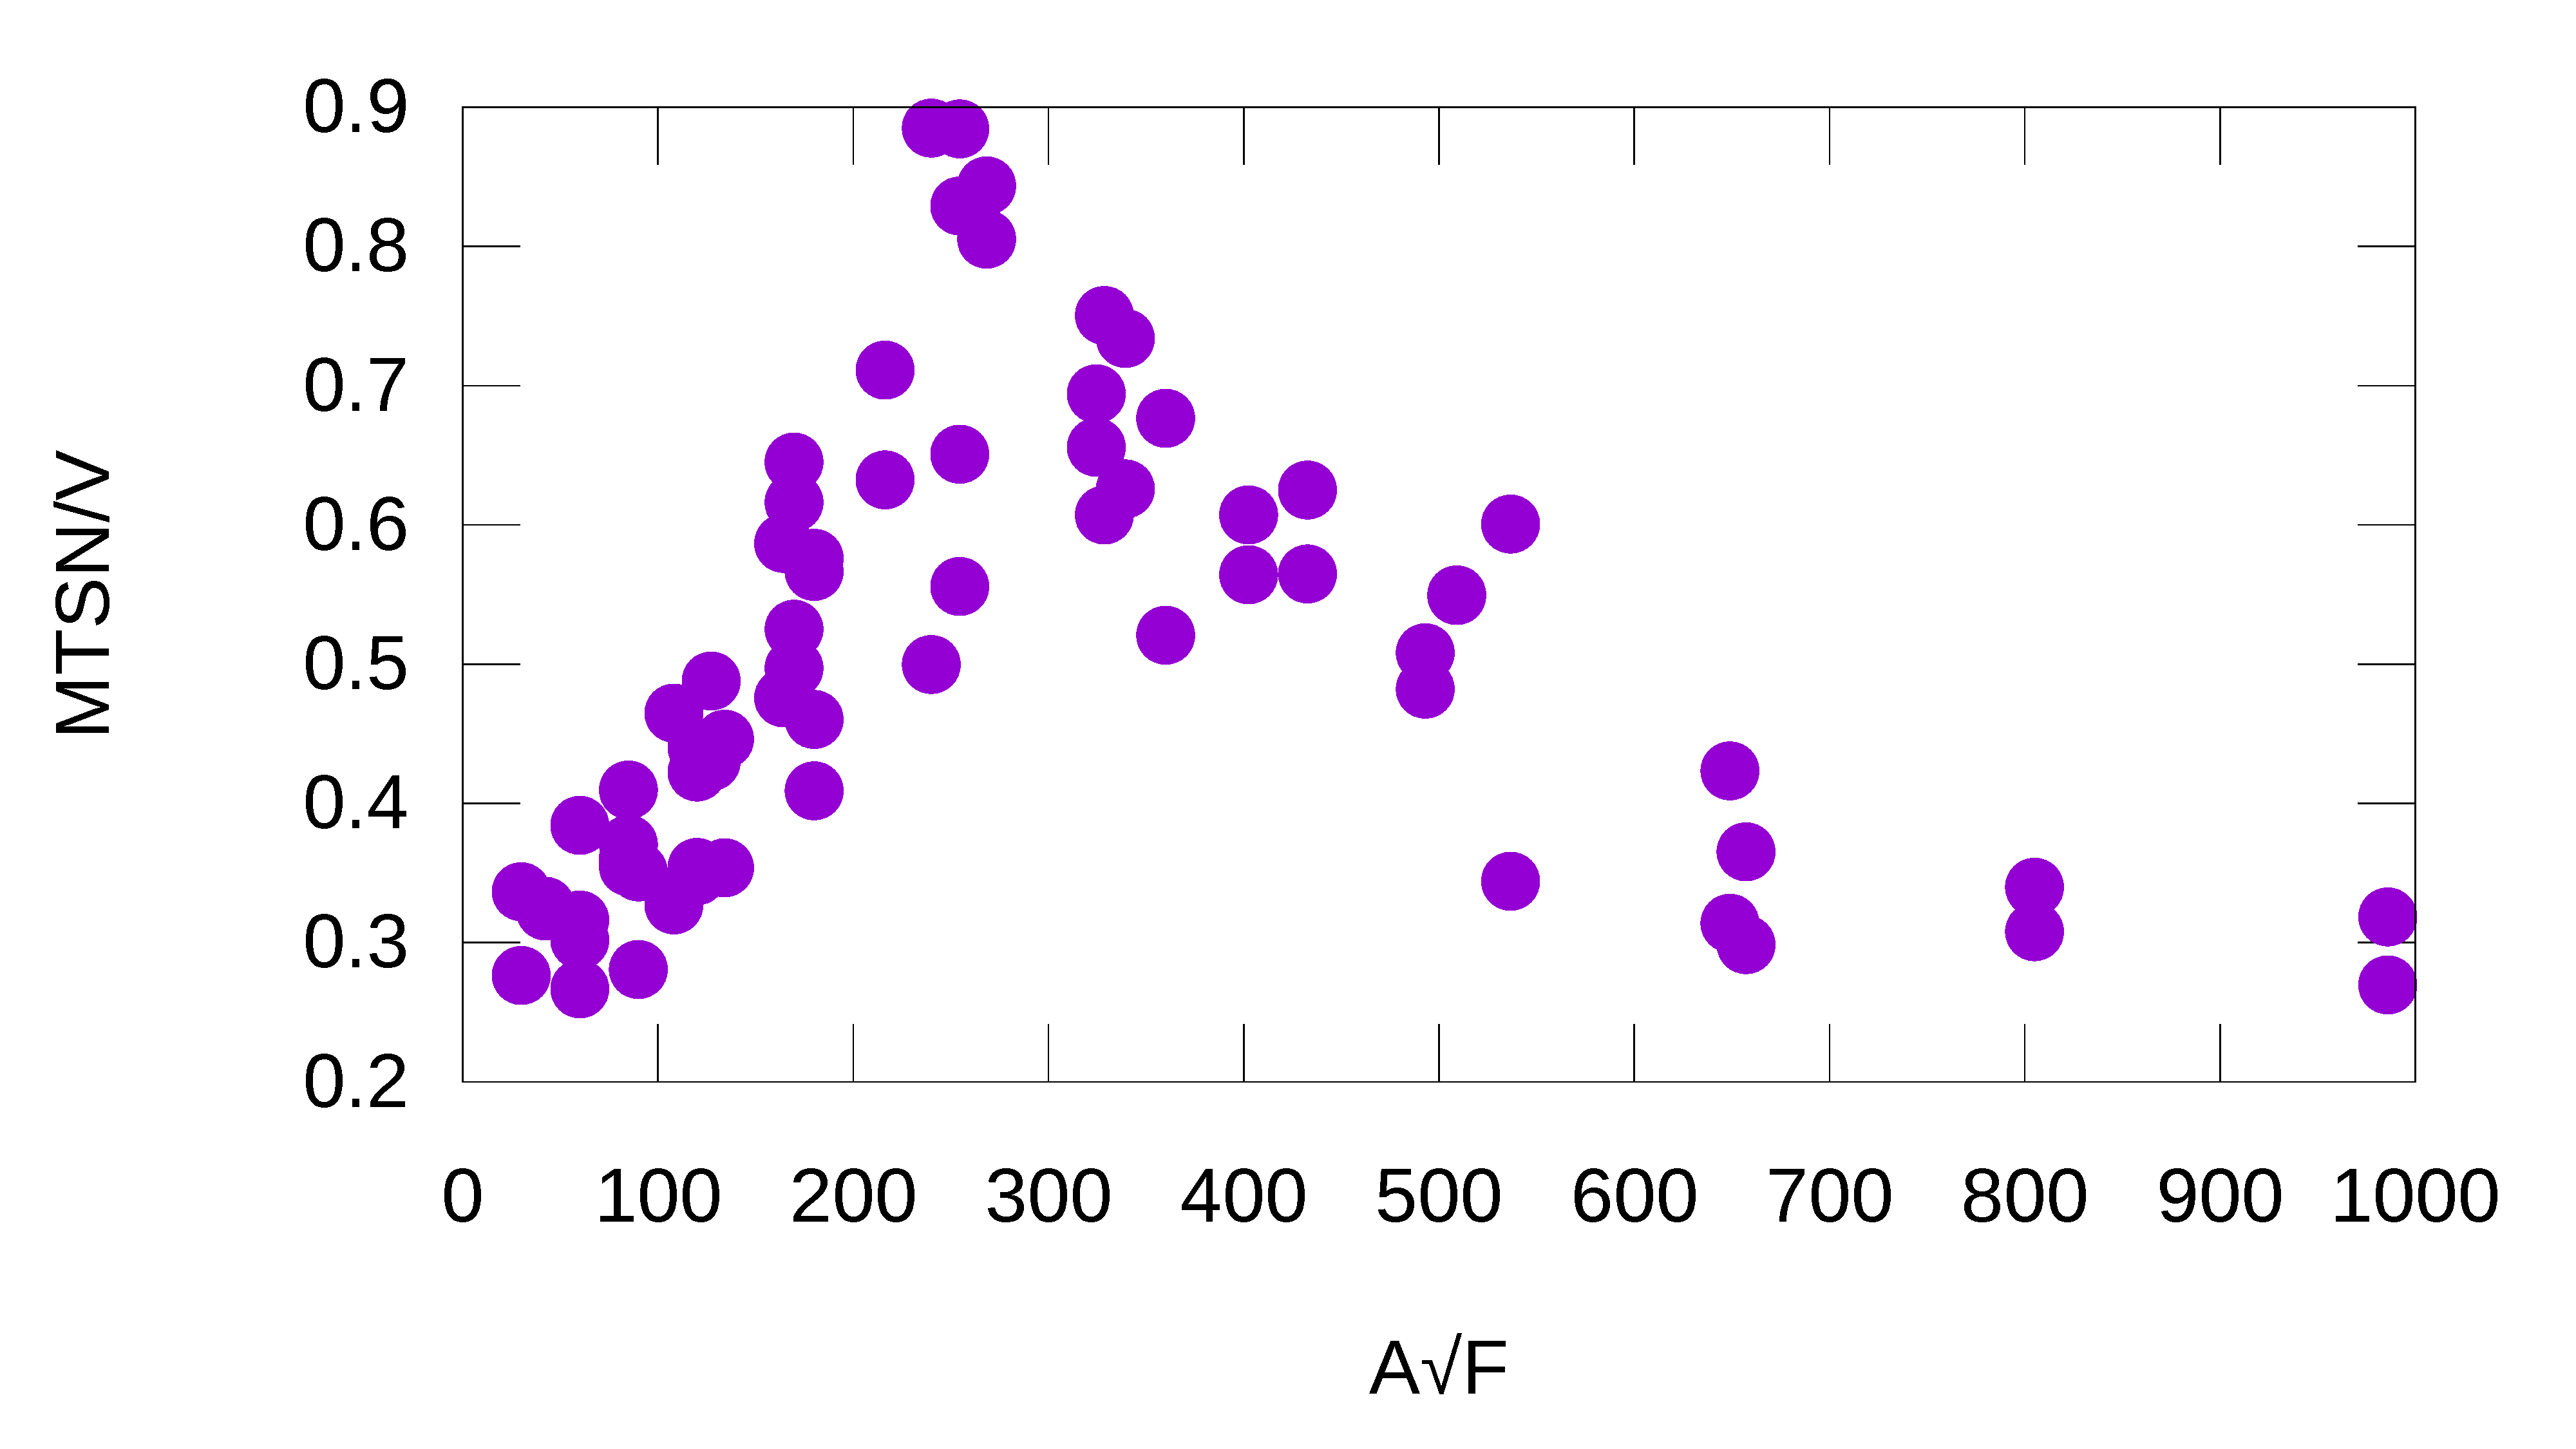
\includegraphics[width=0.7\textwidth]{figures/ch5/asqrtFvTime}
		\caption[MTSN/V en fonction de $A\sqrt{F}$]{Moyennes des temps de sélection normalisés, divisées par la vitesse, en fonction du produit $A\sqrt{F}$, pour des cibles de vitesse moyenne ou rapide.}
		\label{fig:tAsqrtF}
	\end{figure}
	
	Celle-ci nous apprend que lorque la valeur de $A\sqrt{F}$ est autour de 250~$\degree{}Hz^{\frac{1}{2}}$, les temps de sélection sont maximaux. Nous appellerons cette valeur $PES_{max}$. De manière analogue, il est possible de considérer le produit AF, auquel cas cette valeur se trouve autour de 1200~\textdegree{}Hz. Compte tenu des résultats du chapitre 4, il est préférable d'utiliser le produit $A\sqrt{F}$. Nous pouvons donc en tirer une recommandation pratique simple : chercher à s'éloigner de ces valeurs de référence. Ainsi, la conception d'une application impliquant la sélection de cibles mobiles devrait inclure une phase d'estimation de la pseudo-entropie ou, de manière équivalente et peut-être plus pertinente, de $A\sqrt{F}$. Puis, une phase de réflexion sur les manières dont il serait possible de modifier le comportement des cibles pour s'éloigner de la valeur correspondant à la difficulté maximale.
	
	Concrètement, si la valeur de $A\sqrt{F}$ estimée est inférieure à 250, il faudra chercher à diminuer A ou F ; si elle est supérieure, il faudra chercher à les augmenter. Dans un contexte vidéoludique, par exemple, cela implique de modifier les paramètres de mouvement des objets, si cela n'a pas d'effet délétère sur les mécanismes de jeu. Dans d'autres contextes applicatifs, il n'est pas forcément aisé de modifier le comportement intrinsèque des objets. Toutefois, cette recommandation pratique vaut autant pour la conception d'applications que pour l'élaboration de techniques d'aide à la sélection. En effet, certaines des techniques de sélection étudiées dans le chapitre~\ref{chap2} sont fondées sur la modification de la taille effective des cibles ou de leur distance au curseur ; lorsqu'il s'agit de cibles mobiles, elles peuvent également agir sur la vitesse, dont nous savons que l'importance est primordiale.
	
	Dans la plupart des contextes applicatifs que nous avons étudiés, la PES d'une cible est généralement en dessous de $PES_{max}$. Pour l'en éloigner encore plus, il faut donc chercher à diminuer A et F. Bien sûr, cette diminution n'est généralement pas incompatible avec l'usage d'une autre technique d'aide à la sélection, comme par exemple le \emph{Bubble Cursor}~\cite{grossman2005bubble}, ou encore \emph{Hook}~\cite{ortega2013hook}.
	
	\subsection{Modification du paramètre V}
	Des techniques consistant à modifier la vitesse de cibles à sélectionner existent déjà, et deux d'entre elles sont présentées dans la section~\ref{sub:timeLord} : \emph{Hold}~\cite{hajri2011moving} et \emph{Target Ghost}~\cite{hasan2011comet}. La première stoppe le mouvement des cibles, tandis que la seconde ajoute à chaque cible un \emph{proxy} statique, que l'utilisateur peut sélectionner à sa place.
	
	Chacune revient en quelque sorte à arrêter le temps. La vitesse pouvant être définie comme le raport de la distance parcourue par le temps de trajet, il est logique de chercher à manipuler la vitesse en manipulant le temps. Mais jouer sur la distance est également possible, fût-ce indirectement, comme nous les verrons plus loin.
	
	\emph{Hold} a l'inconvénient d'engendrer une perte du contexte dynamique de l'application, et se prête mal aux usages en temps réel. \emph{Target Ghost} est plus souple, mais implique une forte déconnexion entre les \emph{proxies} statiques et leurs cibles-mères respectives, dont les positions deviennent totalement décorrélées.
	
	\subsubsection{\emph{Proxy} ralenti}
	Une solution moins contraignante existe, et consiste à générer un \emph{proxy} mobile, dont la vitesse est bornée par une valeur strictement inférieure à celle de la cible. À chaque instant, le \emph{proxy} se dirige vers la cible qui l'a engendré. Il apparaît immédiatement que, si le mouvement est suffisamment désordonné, même un \emph{proxy} très lent pourra suivre sa cible-mère sans que la distance entre les deux ne diverge ; pour un mouvement plus régulier, la vitesse du \emph{proxy} devra être plus proche de celle de la cible pour éviter cette divergence. Dans ce dernier cas cependant, la régularité du mouvement de la cible implique une sélection plus aisée, de sorte que le gain relativement faible apporté par l'utilisation d'un \emph{proxy} lent n'est pas nécessairement un inconvénient majeur.
	
	\begin{figure}[!htb]
		%\centering
		\begin{subfigure}[t]{0.49\textwidth}
			\centering
			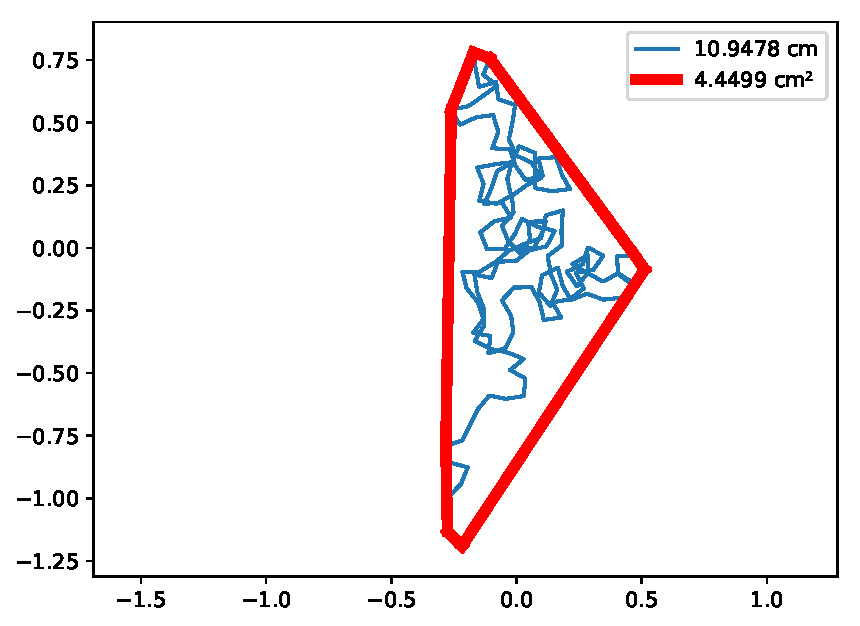
\includegraphics[width=\textwidth]{figures/ch5/2_19_SpeedReduction_2_19_120_32}
			\caption{Trajectoire originale.}
			\label{fig:speedRedOriginal}
		\end{subfigure}
		~
		\begin{subfigure}[t]{0.49\textwidth}
			\centering
			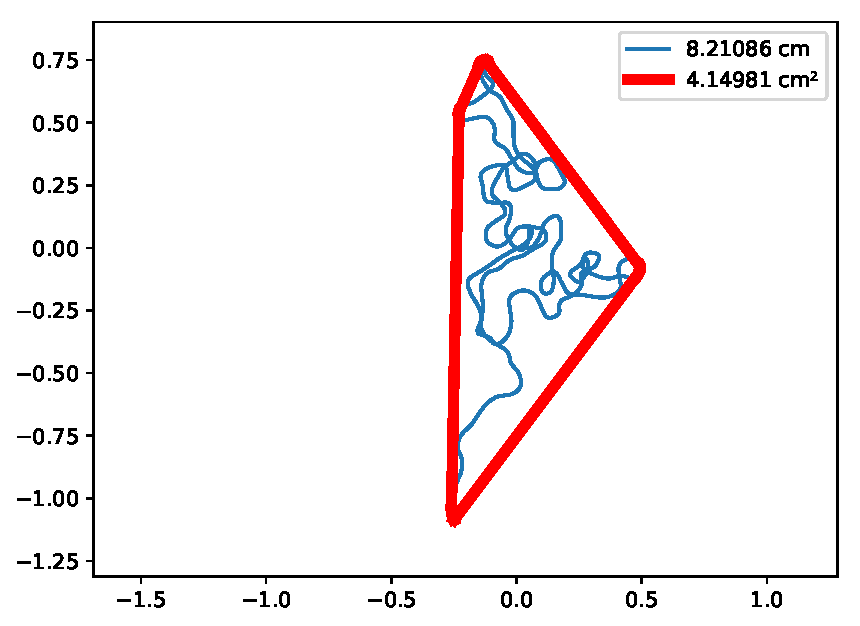
\includegraphics[width=\textwidth]{figures/ch5/2_19_SpeedReduction_2_19_120_32_factor_0_75}
			\caption{Trajectoire filtrée, avec $FR = 75$~\%{}.}
			\label{fig:speedRed075}
		\end{subfigure}
		~
		\begin{subfigure}[t]{0.49\textwidth}
			\centering
			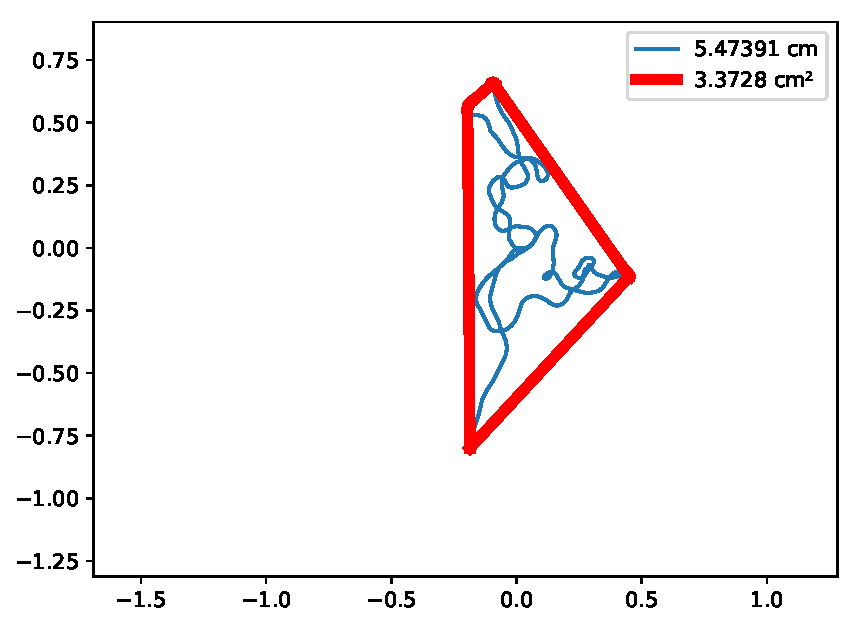
\includegraphics[width=\textwidth]{figures/ch5/2_19_SpeedReduction_2_19_120_32_factor_0_5}
			\caption{Trajectoire filtrée, avec $FR = 50$~\%{}.}
			\label{fig:speedRed050}
		\end{subfigure}
		~
		\begin{subfigure}[t]{0.49\textwidth}
			\centering
			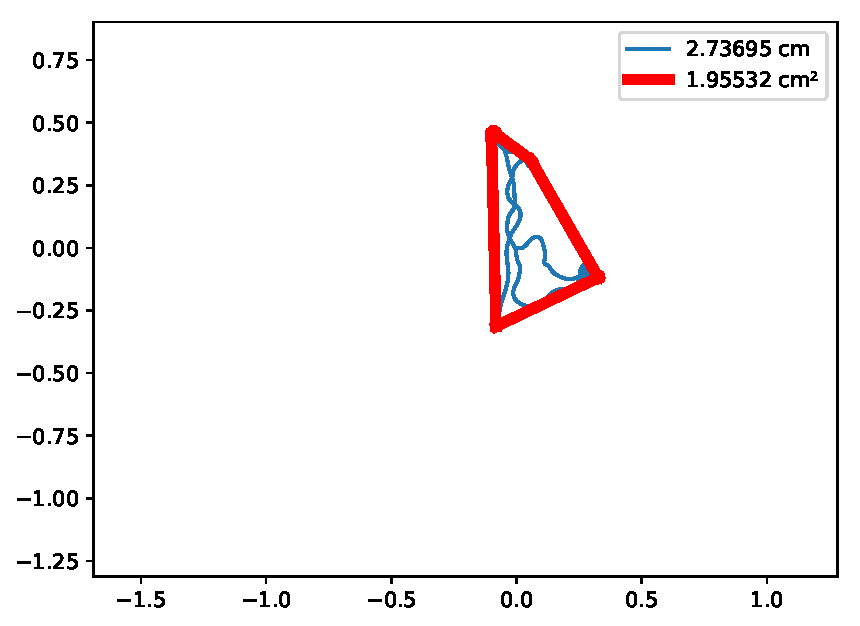
\includegraphics[width=\textwidth]{figures/ch5/2_19_SpeedReduction_2_19_120_32_factor_0_25}
			\caption{Trajectoire filtrée, avec $FR = 25$~\%{}.}
			\label{fig:speedRed025}
		\end{subfigure}
		\caption[Utilisation de \emph{proxies} lents]{Utilisation de \emph{proxies} lents pour faciliter la sélection. Pour la trajectoire originale, V vaut 2,19~cm/s, A vaut 120\textdegree{}, F vaut 32~Hz, et chaque trajectoire est générée sur 5 secondes, comme pour les données du chapitre~\ref{chap4}. Les trois autres trajectoires sont générées avec des facteurs de ralentissement de la cible (FR) indiqués en légende de chaque sous-figure. En bleu, les trajectoires avec leurs longueurs respectives indiquées en légende ; en rouge, les aires de leurs enveloppes convexes.}
		\label{fig:speedRed}
	\end{figure}
	
	Des exemples de \emph{proxies} lents sont fournis sur la figure~\ref{fig:speedRed}. Pour les paramètres VFA étudiés ici, l'utilisation d'un \emph{proxy} limité à 75~\%{} de la vitesse de sa cible-mère permet de conserver l'allure générale de la trajectoire originale, sans trop affecter son enveloppe convexe, et en la lissant quelque peu, au point de donner une allure ciné-continue au mouvement généré (revoir la section~\ref{sub:kinematicTypes} pour la définition de ce terme). Du fait de la réduction de la vitesse et du lissage opéré, rendant le mouvement un peu plus prévisible, le \emph{proxy} est plus aisé à sélectionner.
	
	Néanmoins, l'application d'une réduction de vitesse plus forte, ne serait-ce que de 50~\%{}, introduit un décalage important entre la cible et son \emph{proxy}, ce que la forme et l'aire de l'enveloppe convexe illustrent ; le phénomène n'en est que plus marqué lorsque le facteur de réduction de vitesse est de 25~\%{}. C'est ce qu'illustre la figure~\ref{fig:filteringBySpeedRed}, sur laquelle on observe malgré tout une forte augmentation de l'aire de l'enveloppe convexe divisée par la vitesse au carré, ce qui s'explique par la diminution de la vitesse. Or, les données présentées sur la figure~\ref{fig:perf_V_RealArea_normed} (section~\ref{sub:areaVperf}) montrent que quand cette valeur est très grande, la sélection est généralement rapide. Par ailleurs, les résultats présentés sur la figure~\ref{fig:perf_V_RealArea_raw} de la même section montrent que lorsque la vitesse est faible, les temps de sélection sont toujours relativement courts de toute manière.



	\begin{figure}[!htb]
		%\centering
		\begin{subfigure}[t]{0.49\textwidth}
			\centering
			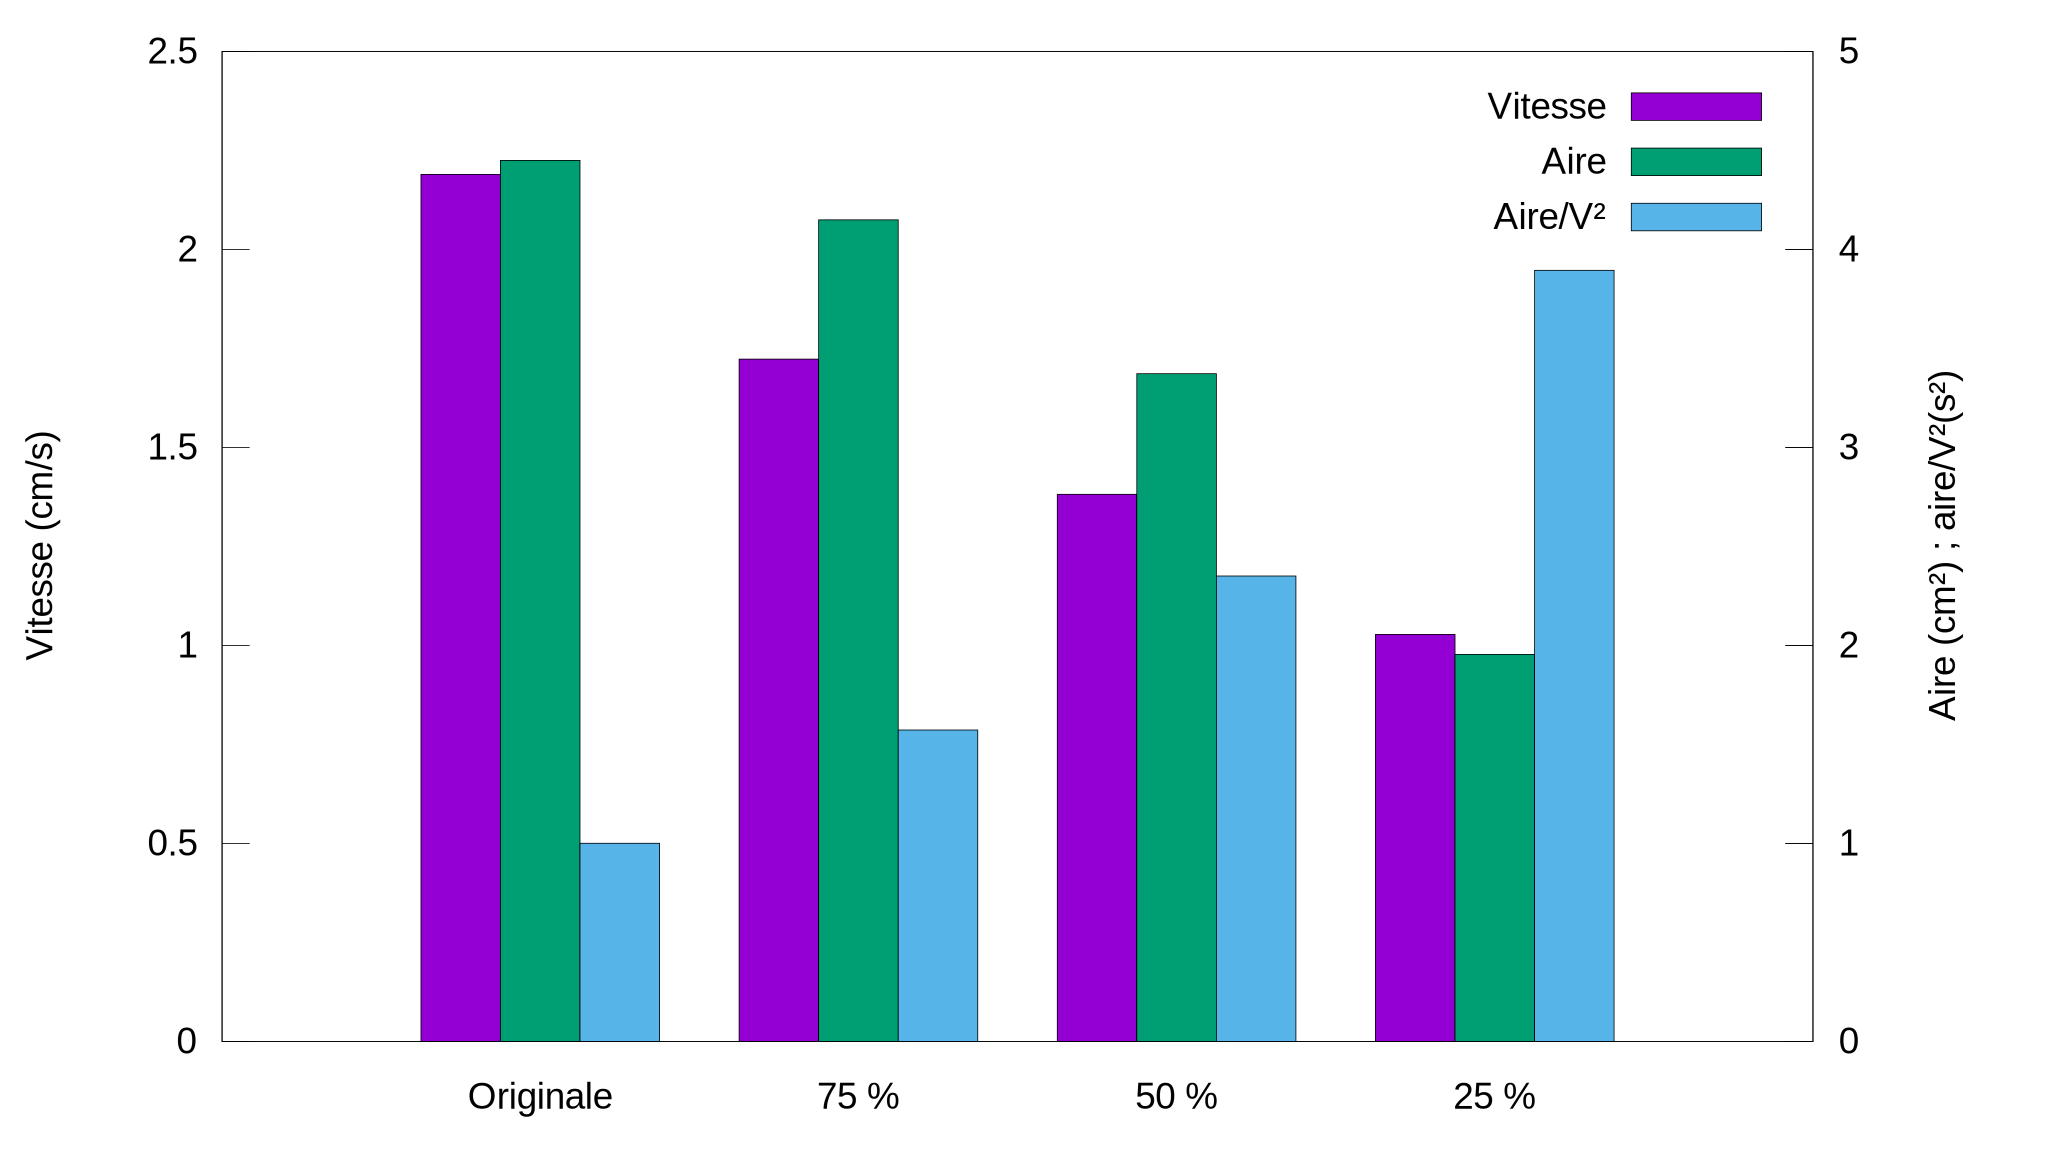
\includegraphics[width=\textwidth]{figures/ch5/filteringBySpeedRedHistograms}
			\caption{\emph{Proxy} lent. La vitesse est naturellement proportionnelle au facteur de ralentissement appliqué. L'aire de l'enveloppe convexe demeure à peu près stable quand RF vaut 75~\%{}, mais chute fortement au-delà.}
			\label{fig:filteringBySpeedRed}
		\end{subfigure}
		~
		\begin{subfigure}[t]{0.49\textwidth}
			\centering
			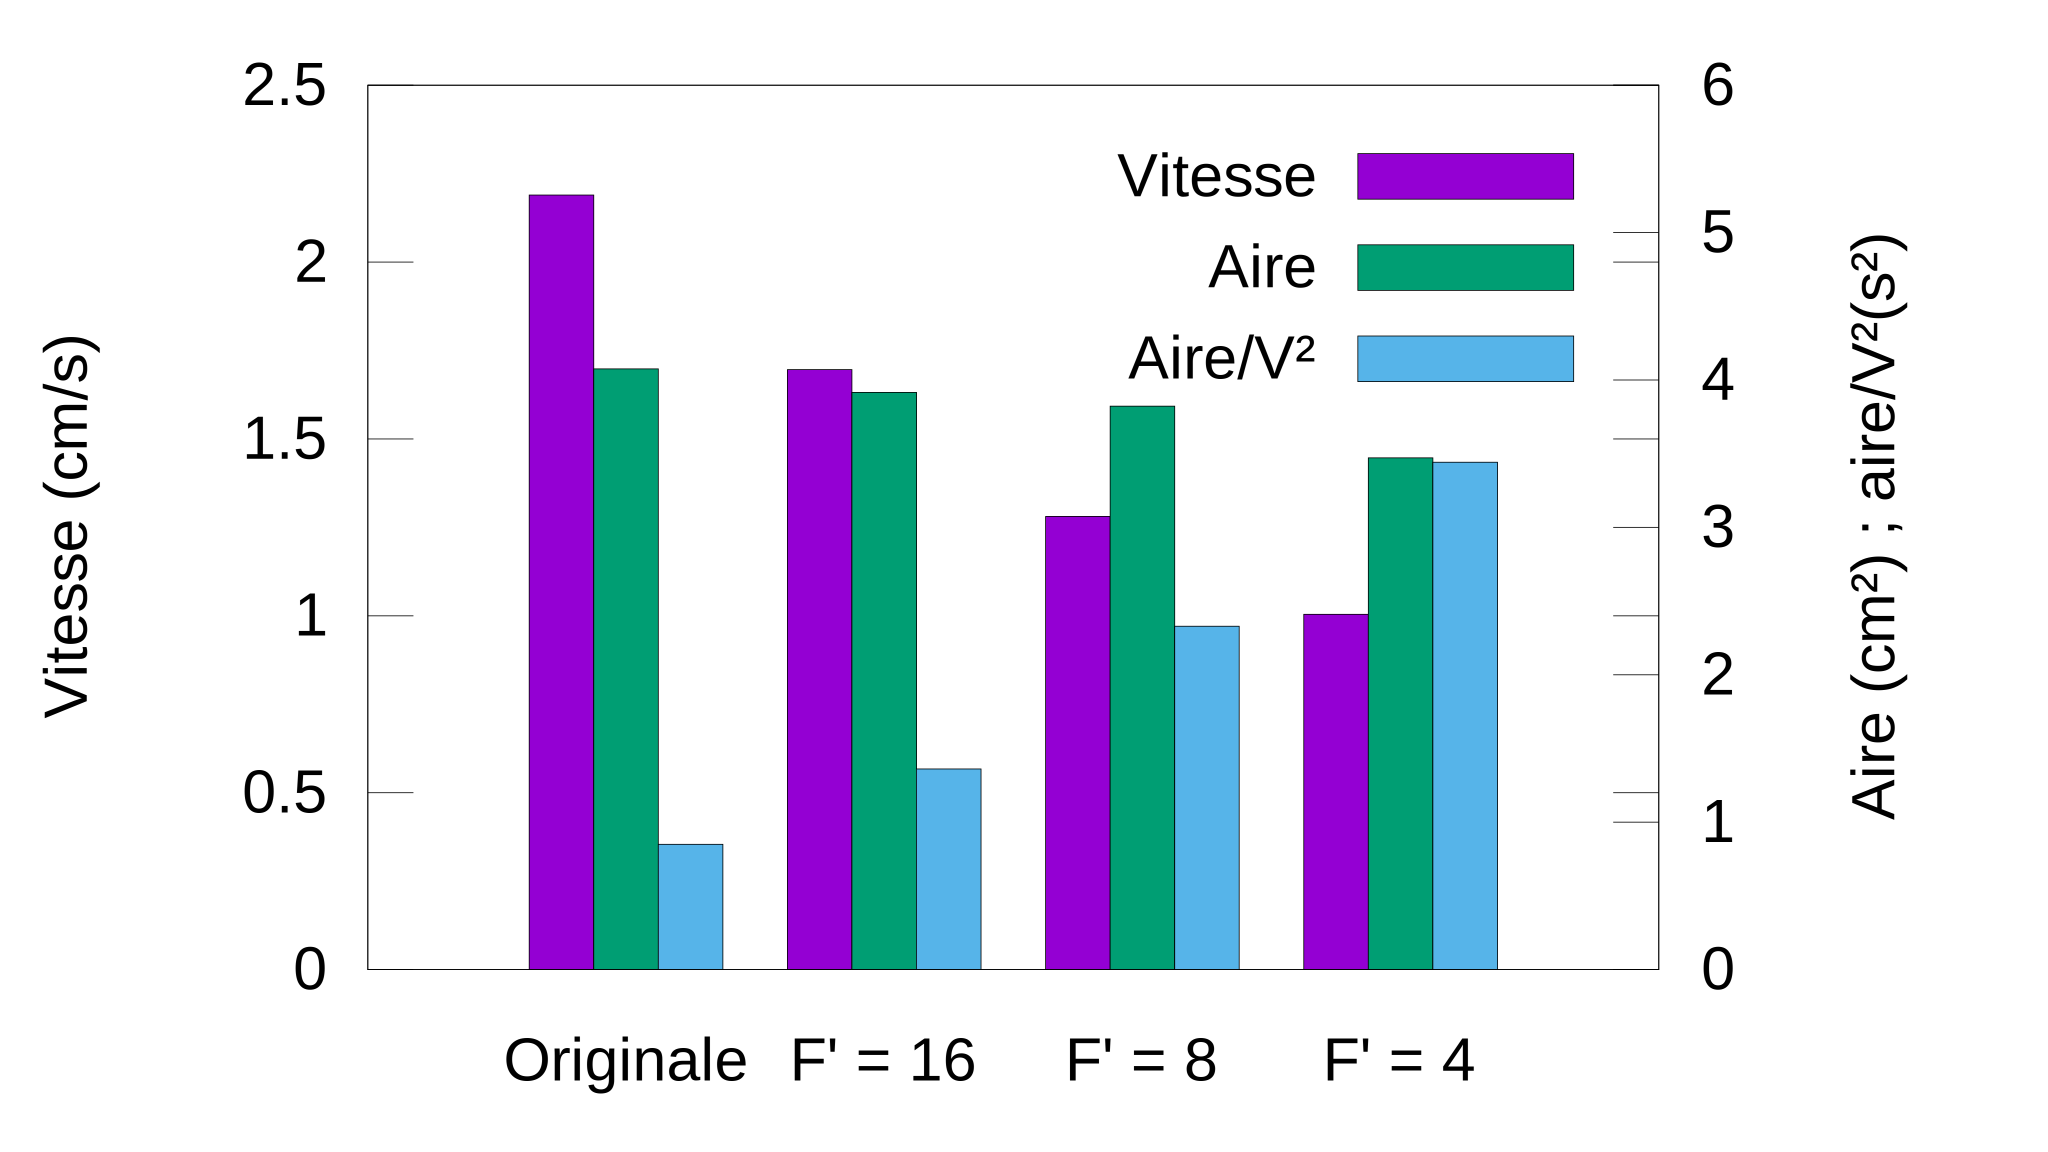
\includegraphics[width=\textwidth]{figures/ch5/filteringByFHistograms}
			\caption{Filtrage fréquentiel. La trajectoire se trouve modifiée de telle manière que la vitesse moyenne de la cible chute drastiquement --- de 2,19~cm/s à 1,00~cm/s --- de même, évidemment, que la fréquence. L'aire de l'enveloppe convexe demeure relativement stable.}
			\label{fig:filteringByFHistograms}
		\end{subfigure}
		\caption[Effet de modifications du comportement des cibles]{Effet de modifications du comportement des cibles sur les caractéristiques des trajectoires. Les trajectoires sont générées avec $V=2,19~cm/s$, $F=32~Hz$, et $A=120\degree{}$.}
		\label{fig:speedRedAndFilteringbyFhistograms}
	\end{figure}
	
	D'autres combinaisons de VFA engendrant un mouvement plus \og brownien \fg{} toléreraient mieux de fortes réductions de vitesse, et sans doute certains contextes applicatifs seraient-ils propices à de fortes réductions, quitte à introduire un grand décalage --- potentiellement divergent --- entre une cible et son \emph{proxy}. En somme, l'utilisation d'un \emph{proxy} lent peut fortement faciliter la sélection, à condition que le contexte applicatif tolère les modifications du comportement de la cible qu'elle implique.
	
	\subsection{Modification du paramètre F}
	Il est difficile d'imaginer une façon d'augmenter la valeur de F qui ait du sens, à l'exception, peut-être, du choix d'une plus haute fréquence d'échantillonage, lorsqu'il s'agit de données mesurées ou simulées, par exemple pour un enregistrement vidéo, ou une simulation scientifique impliquant des particules.
	
	Toutefois, une option permettant de réduire le paramètre F est d'appliquer un filtrage, par exemple de façon analogue à ce qu'opérerait un filtre passe-bas. La conception d'une telle technique d'assistance à la sélection serait différente selon le degré d'intégration à l'application : avec une intégration forte, il serait possible de modifier directement le comportement des cibles ; avec une intégration faible, il faudrait se contenter d'ajouter un \emph{proxy}, comme le fait la technique \emph{Ghost}~\cite{hasan2011comet}. Ce procédé a par ailleurs l'avantage d'éviter de perdre les informations concernant les positions exactes des cibles potentielles, au prix d'un encombrement visuel accru.
	
	\subsubsection{Filtrage avec limitation à 4~Hz}
	Illustrons notre propos par un exemple concret de technique d'aide à la sélection, fondée sur une limitation de la fréquence de changements de direction à 4~Hz --- ce choix est quelque peu arbitraire, mais informé par les données de la figure~\ref{fig:fEffectPerf}, section~\ref{sub:freqEffect}. Si une cible a un paramètre F dont la valeur intrinsèque est de 32~Hz, un \emph{proxy} de la cible est créé, mais sa position n'est mise à jour que quatre fois par seconde ; les valeurs intérmédiaires étant interpolées. Cette méthode a l'avantage de permettre au \emph{proxy}, dans une certaine mesure, de \og coller \fg{} aux mouvements de la cible réelle, mais de manière moins saccadée, plus prévisible.
	
	Cela se fait toutefois au prix d'une latence inversement proportionnelle à la fréquence d'échantillonage choisie (que nous appelons $F'$), c'est-à-dire ici $\frac{1}{4}~s = 250~ms$. Naturellement, il est possible de réduire cette latence en augmentant la fréquence d'échantillonage, ce qui a l'inconvénient de diminuer l'efficacité de la technique. Cette façon de filtrer les positions des cibles permet de conserver des points en commun avec la trajectoire initiale, et donc de ne pas trop en modifier l'étendue et l'allure générale, comme l'illustre la figure~\ref{fig:filterF}.
	
	\begin{figure}[!htb]
		%\centering
		\begin{subfigure}[t]{0.49\textwidth}
			\centering
			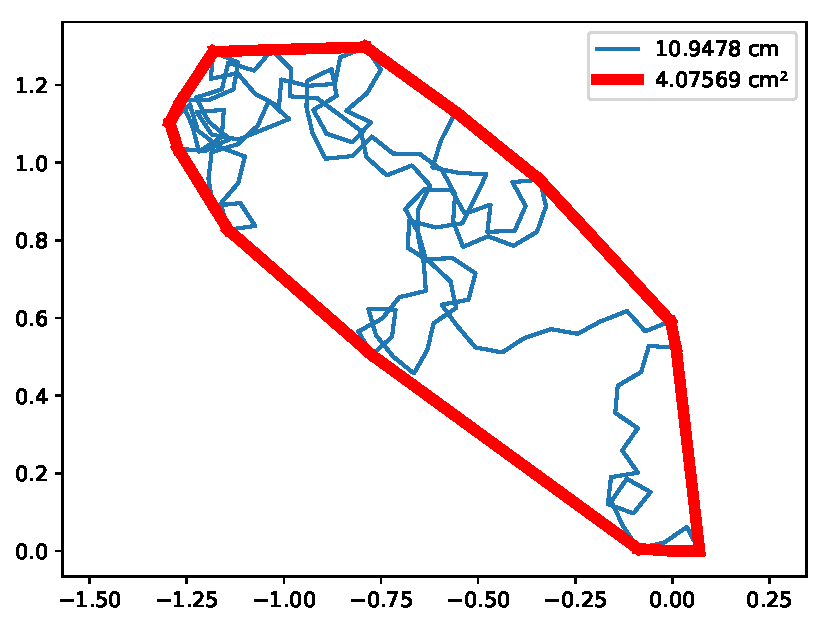
\includegraphics[width=\textwidth]{figures/ch5/2_19_freqFilter_2_19_120_32}
			\caption{Trajectoire originale, $F = 32$~Hz.}
			\label{fig:filterFnoFilter}
		\end{subfigure}
		~
		\begin{subfigure}[t]{0.49\textwidth}
			\centering
			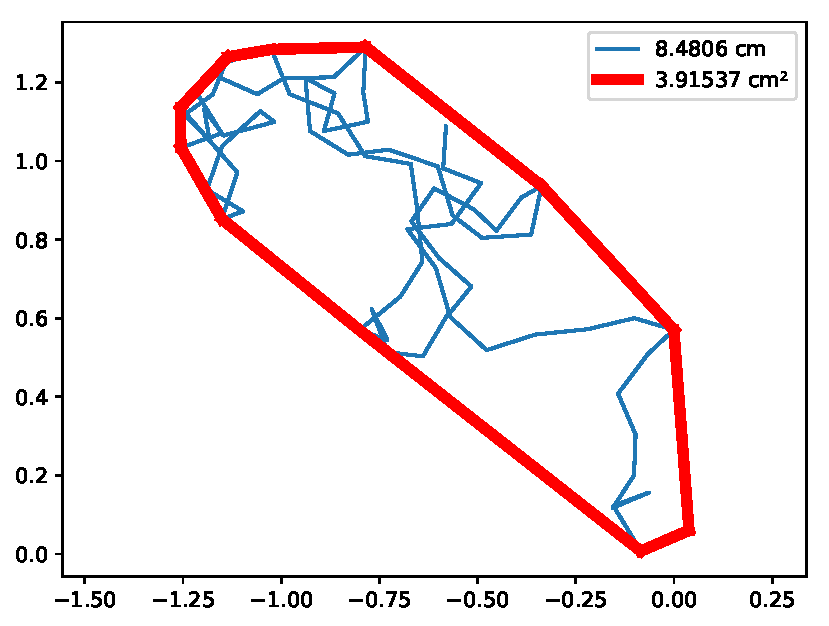
\includegraphics[width=\textwidth]{figures/ch5/2_19_freqFilter_2_19_120_32_filter_16}
			\caption{Trajectoire filtrée, avec $F' = 16$~Hz.}
			\label{fig:filterFw16}
		\end{subfigure}
		~
		\begin{subfigure}[t]{0.49\textwidth}
			\centering
			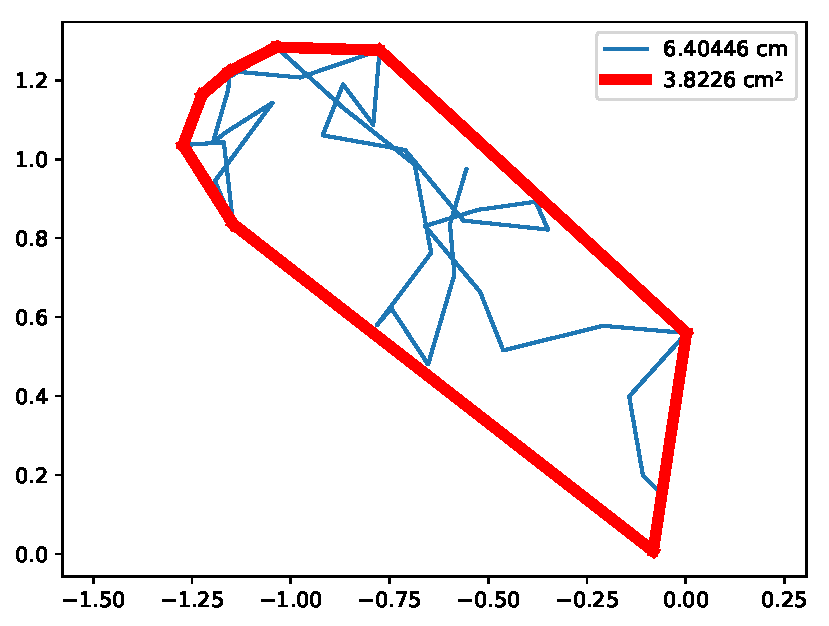
\includegraphics[width=\textwidth]{figures/ch5/2_19_freqFilter_2_19_120_32_filter_8}
			\caption{Trajectoire filtrée, avec $F' = 8$~Hz.}
			\label{fig:filterFw8}
		\end{subfigure}		
		~
		\begin{subfigure}[t]{0.49\textwidth}
			\centering
			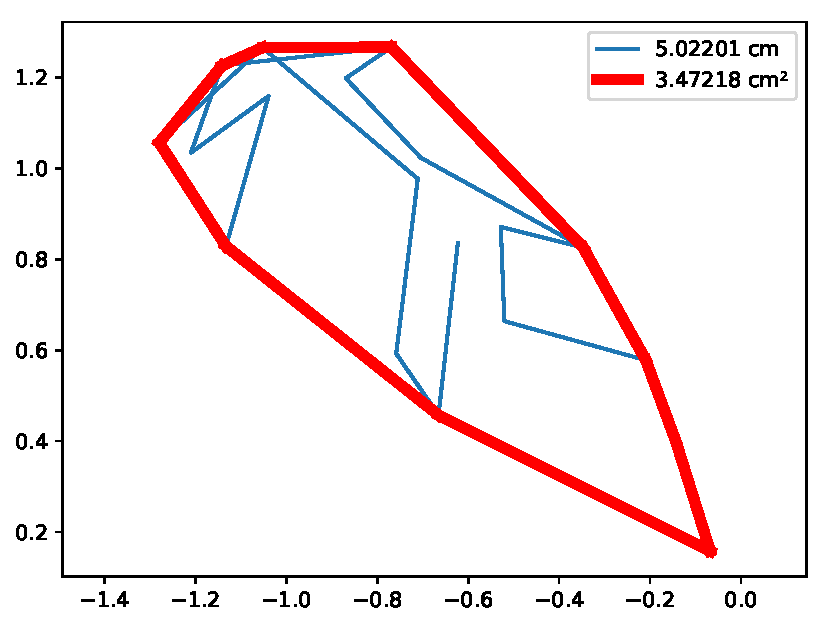
\includegraphics[width=\textwidth]{figures/ch5/2_19_freqFilter_2_19_120_32_filter_4}
			\caption{Trajectoire filtrée, avec $F' = 4$~Hz.}
			\label{fig:filterFw4}
		\end{subfigure}
		\caption[Filtrage des trajectoires par limitation de fréquence]{Une trajectoire originale, et trois trajectoires produites par limitation de la fréquence. Pour la trajectoire originale, A vaut 120\textdegree{}, et chaque trajectoire est générée sur 5 secondes, comme pour les données du chapitre~\ref{chap4}. Le paramètre A n'est pas nécessairement respecté pour les trajectoires filtrées, attendu que plusieurs angles de 120\textdegree{} au plus peuvent s'accumuler d'une période à l'autre. En bleu, les trajectoires avec leurs longueurs respectives indiquées en légende ; en rouge, les aires de leurs enveloppes convexes.}
		\label{fig:filterF}
	\end{figure}
	
	\paragraph{Effet secondaire sur la vitesse des cibles.}
	Mais un effet secondaire de ce procédé est crucial : la longueur de la trajectoire est réduite. Or, attendu que la durée totale du mouvement n'est pas modifiée (elle est de 4 secondes pour les trajectoires de la figure~\ref{fig:filterF}), la vitesse moyenne de la cible diminue. Or, nous l'avons vu plus haut, la vitesse est le paramètre dont l'effet sur les temps de sélection est le plus fort, ainsi que le plus simple. En effet, les temps de sélection dépendent de la vitesse de façon approximativement affine, et les taux d'erreur, de façon approximativement linéaire (voir la figure~\ref{fig:spEffectPerf}, section~\ref{sub:spEffect}).
	
	L'effet du filtrage par fréquence sur la vitesse des cibles est illustré sur la figure~\ref{fig:filteringByFHistograms}. On y constate qu'une forte diminution de la vitesse (jusqu'à -54,34~\%{}) accompagne celle de la fréquence. L'aire de l'enveloppe convexe, elle, demeure relativement stable, avec une diminution de 14,8~\%{} seulement dans le cas le plus extrème, avec $F'=4~Hz$. Mais comme la vitesse diminue, l'aire divisée par la vitesse au carrée augmente fortement. Or, quand cette valeur est très grande, la sélection est généralement rapide, lorsque la vitesse est faible, elle l'est toujours.
	
	Il en résulte que si l'allure générale de la trajectoire, ainsi que l'espace qu'elle occupe ne changent guère, la cible devient considérablement plus aisée à sélectionner, d'après nos modèles. Comme la figure~\ref{fig:fEffectPerf} l'illustre, la réduction de la fréquence permet d'améliorer les performances, mais cette réduction est moins perceptible lorsque le paramètre A est particulièrement grand.

	\subsection{Modification du paramètre A}
	Dans ces cas-là, il peut être plus judicieux de chercher à diminuer ce dernier --- là encore, il paraît difficile de chercher à l'augmenter de manière sensée. La réduction du paramètre A est peut-être plus délicate que celle de F, attendu qu'elle ne se prête pas à un filtrage temporel. Certes, s'il est possible de modifier directement le comportement des objets, alors la réduction de A peut s'avérer possible dans certaines circonstances, à condition qu'elle n'ait pas d'impact trop négatif sur l'application concernée.
	
	\subsubsection{Report de la pseudo-entropie sur F}
	Pour rappel, les paramètres A et F ne sont pas égaux dans leur influence sur les performances de sélection, puisque c'est la racine carrée de F dont l'influence est primordiale, et non F lui-même. Par conséquent, il peut être judicieux de diminuer A et d'augmenter F proportionnellement, pour compenser, et maintenir une pseudo-entropie constante, si le contexte applicatif l'exige.
	
	Supposons en effet une cible dont la pseudo-entropie subjective est la \og pire \fg{} possible, soit $A\sqrt{F} = PES_{max} = 250$, avec $A = 50~; F = 25~; \sqrt{F} = 5~; AF = 1250$. S'il on veut conserver la même quantité de désordre sur une durée donnée, il faut maintenir le produit AF constant à 250. Pour ce faire, nous pouvons, par exemple, diviser A par 2, et multiplier F par le même nombre, ce qui aboutit à la situation suivante : $A = 25~; F = 50~; \sqrt{F} \approx 7,07$ ; d'où $A\sqrt{F} \approx 176,78$, soit une diminution de la PES qui l'éloigne de $PES_{max}$.
	
	Naturellement, l'effet est d'autant plus fort que le facteur choisi est élevé ; ainsi, avec 5, nous obtenons les valeurs suivantes : $A = 10~; F = 125~; \sqrt{F} \approx 11,18~; A\sqrt{F} \approx 111,80$. La figure~\ref{fig:tAsqrtF} montre que pour ces valeurs de PES, les performances de sélection sont bien meilleures que pour $PES_{max}$. Néanmoins, tous les dispositifs d'affichage ne sont pas capables d'atteindre de telles fréquences, ce qui limite la portée de cette approche.
	
	\subsubsection{Limitation de A avec compensation ultérieure}
	Une autre option consiste à imposer une limite ferme à la cible (ou à son \emph{proxy}) et à chercher à compenser à chaque nouveau changement de direction. Supposons par exemple une borne de 30\textdegree{} imposée au paramètre A, et un proxy représentant chaque cible. Pour une cible donnée, si son vecteur vitesse subit à un instant $t$ une rotation de plus de 30\textdegree{}, son \emph{proxy} ne voit son vecteur vitesse tourner que de 30\textdegree{}. Lors du prochain changement de direction du vecteur vitesse, celui du proxy est alors ajusté non pas de manière à correspondre à la nouvelle rotation subie par le vecteur vitesse réelle, mais de manière à orienter le proxy dans la direction de la cible qu'il représente, pour compenser le décalage induit par l'imposition d'une borne sur A. Cette compensation se fait néanmoins toujours avec au plus une rotation de 30\textdegree{}. Cette opération est possible sans que la distance entre la cible et son \emph{proxy} ne diverge, car les changements de direction limitent la distance totale parcourue par un objet sur une période et à une vitesse données, attendu que c'est en allant tout droit que l'on s'éloigne le plus de son point de départ.
	
	Néanmoins, selon le paramètre A intrinsèque de la cible, et selon la borne imposée, le comportement du \emph{proxy} peut-être plus ou moins déconnecté de celui de la cible potentielle qu'il représente ; aussi la prudence est-elle de mise lorsque cette technique est mise en œuvre, et il est probablement souhaitable d'éviter d'avoir un écart trop important entre la valeur originelle de A et la borne choisie. Il est toutefois possible de combiner cette imposition de borne avec le report de l'entropie sur F.
	
	\subsection{Filtrage par moyenne mobile}
	La moyenne mobile constitue un type de filtrage passe-bas assez classique. Elle consiste, pour une largeur L, à remplacer chaque valeur $x_{i}$ rencontrée dans une série par la moyenne d'un échantillon de L valeurs centré sur $x_{i}$. Là encore, une latence est introduite par le procédé, et elle est proportionnelle à L. Il serait probablement mal avisé de chercher à lisser ainsi les angles de rotation du vecteur vitesse d'une cible, car cela introduirait un décalage potentiellement divergent entre la position de la cible et celle de son \emph{proxy}. Cependant, il est possible d'appliquer un tel filtrage aux positions mêmes de la cible. Dans ce cas, la trajectoire est considérablement lissée, et ne présente plus d'angles marqués --- elle devient courbe. Ainsi, le mouvement devient ciné-continu, comme l'illustre la figure~\ref{fig:movingAverageTrajs}.
	
	\begin{figure}[!htb]
		%\centering
		\begin{subfigure}[t]{0.49\textwidth}
			\centering
			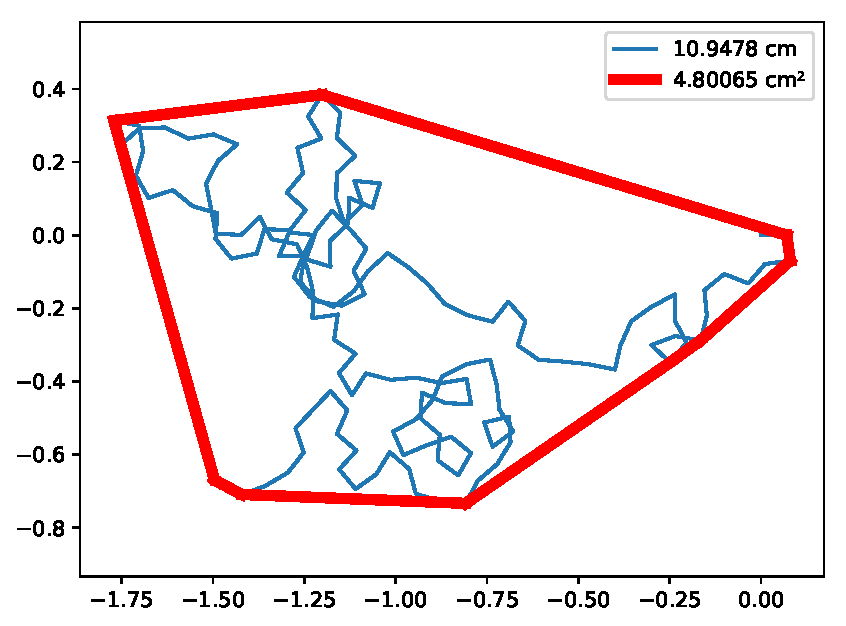
\includegraphics[width=\textwidth]{figures/ch5/2_19_MovingAverage_2_19_120_32}
			\caption{Trajectoire originale.}
			\label{fig:movAvOriginal}
		\end{subfigure}
		~
		\begin{subfigure}[t]{0.49\textwidth}
			\centering
			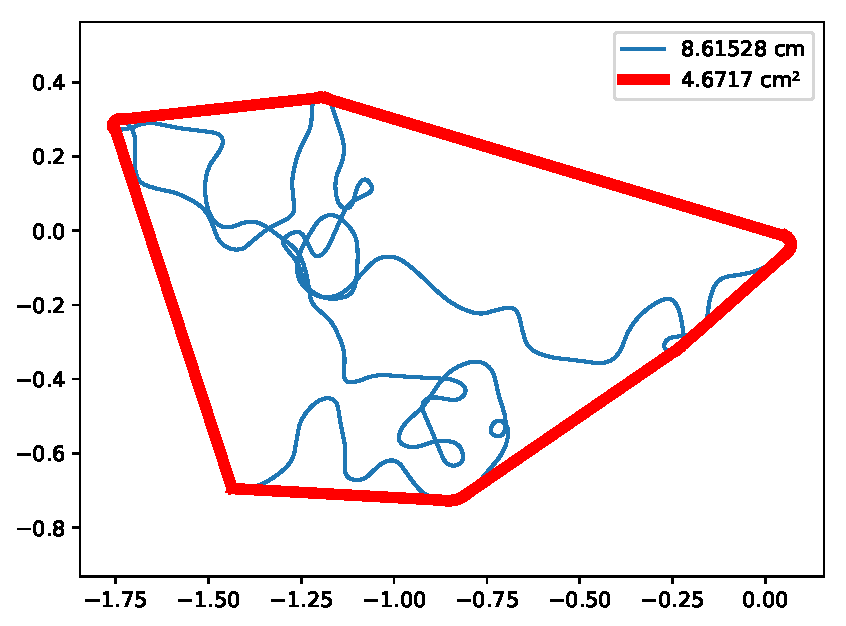
\includegraphics[width=\textwidth]{figures/ch5/2_19_MovingAverage_2_19_120_32_window_62_5}
			\caption{Trajectoire filtrée, avec $L = 62,5$~ms.}
			\label{fig:movAv0625}
		\end{subfigure}
		~
		\begin{subfigure}[t]{0.49\textwidth}
			\centering
			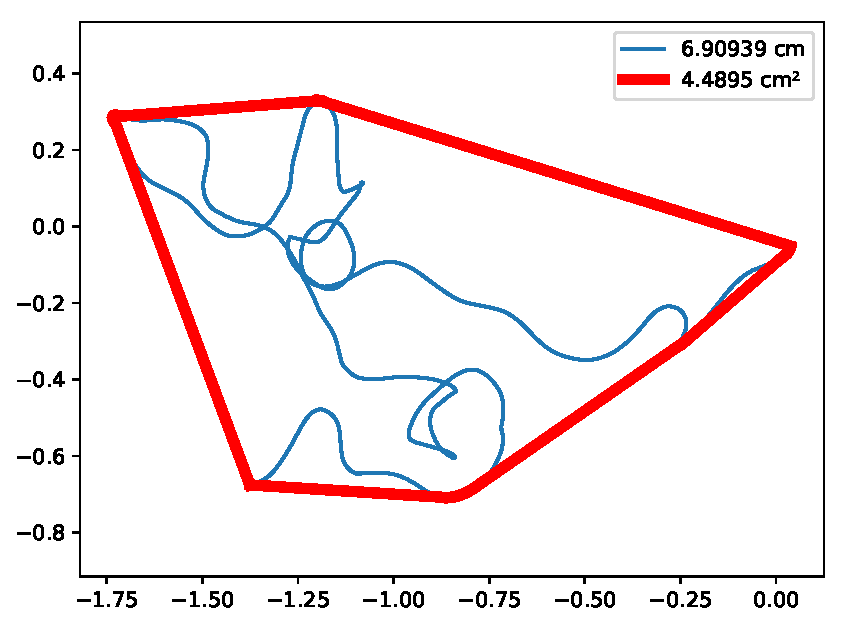
\includegraphics[width=\textwidth]{figures/ch5/2_19_MovingAverage_2_19_120_32_window_125_0}
			\caption{Trajectoire filtrée, avec $L = 125$~ms.}
			\label{fig:movAv1250}
		\end{subfigure}		
		~
		\begin{subfigure}[t]{0.49\textwidth}
			\centering
			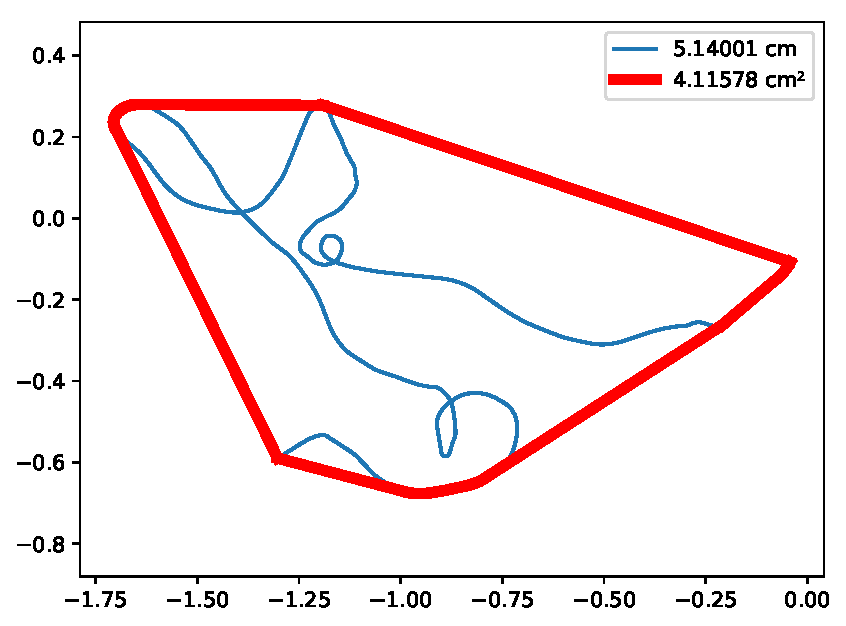
\includegraphics[width=\textwidth]{figures/ch5/2_19_MovingAverage_2_19_120_32_window_250_0}
			\caption{Trajectoire filtrée, avec $L = 250$~ms.}
			\label{fig:movAv2500}
		\end{subfigure}
		\caption[Filtrage des trajectoires par moyenne mobile]{Une trajectoire originale, et trois trajectoires produites par application d'une moyenne mobile sur les positions de la cible. Pour la trajectoire originale, A vaut 120\textdegree{}, tandis que F est de 32~Hz. Chaque trajectoire est générée sur 5 secondes, comme pour les données du chapitre~\ref{chap4}. En bleu, les trajectoires avec leurs longueurs respectives indiquées en légende ; en rouge, les aires de leurs enveloppes convexes. Les largeurs L des fenêtres mobiles sont ici choisies avec 62,5, 125, et 250~ms, car ces durées, si ont les ramène à des fréquences, correspondent respectivement à 16, 8, et 4~Hz, soit les valeurs choisies pour illustrer le filtrage fréquentiel (figure~\ref{fig:filterF}).}
		\label{fig:movingAverageTrajs}
	\end{figure}
	
	De même que pour le filtrage fréquentiel, l'allure générale de la trajectoire, son étendue, et l'aire de son enveloppe convexe ne sont pas significativement modifiées. En revanche, si le filtrage fréquentiel tend à accentuer les angles --- et donc le caractère ciné-discret du mouvement --- la moyenne mobile produit une trajectoire \emph{lissée}, donc ciné-continue. En remplaçant les grands changement de direction instantanés par de petits changements continus, elle rend le mouvement d'une cible plus prévisible, tout en réduisant significativement sa vitesse. Le paramètres A et F n'ont donc ici plus guère de sens, à moins d'en adopter une définition plus adaptée aux mouvements ciné-continus.
	
	Ces effets sont quantifiés sur la figure~\ref{fig:filteringByMovingAverageHistograms}. Les différences sur ces métriques ne sont pas suffisamment marquées pour faire une distinction claire entre le filtrage fréquentiel et l'application d'une moyenne mobile. Cependant, les natures profondément différentes des trajectoires générées (ciné-discrètes dans le premier cas, ciné-continues dans le second) justifient la coexistence de ces deux techniques, dont chacun pourra juger de la pertinence, selon l'application visée. De même, un compromis entre le \og pouvoir \fg{} de lissage et la latence proportionnelle à L doit être trouvé de manière \emph{ad hoc}, selon le contexte applicatif.
	
	\begin{figure}[!htb]
		\centering
		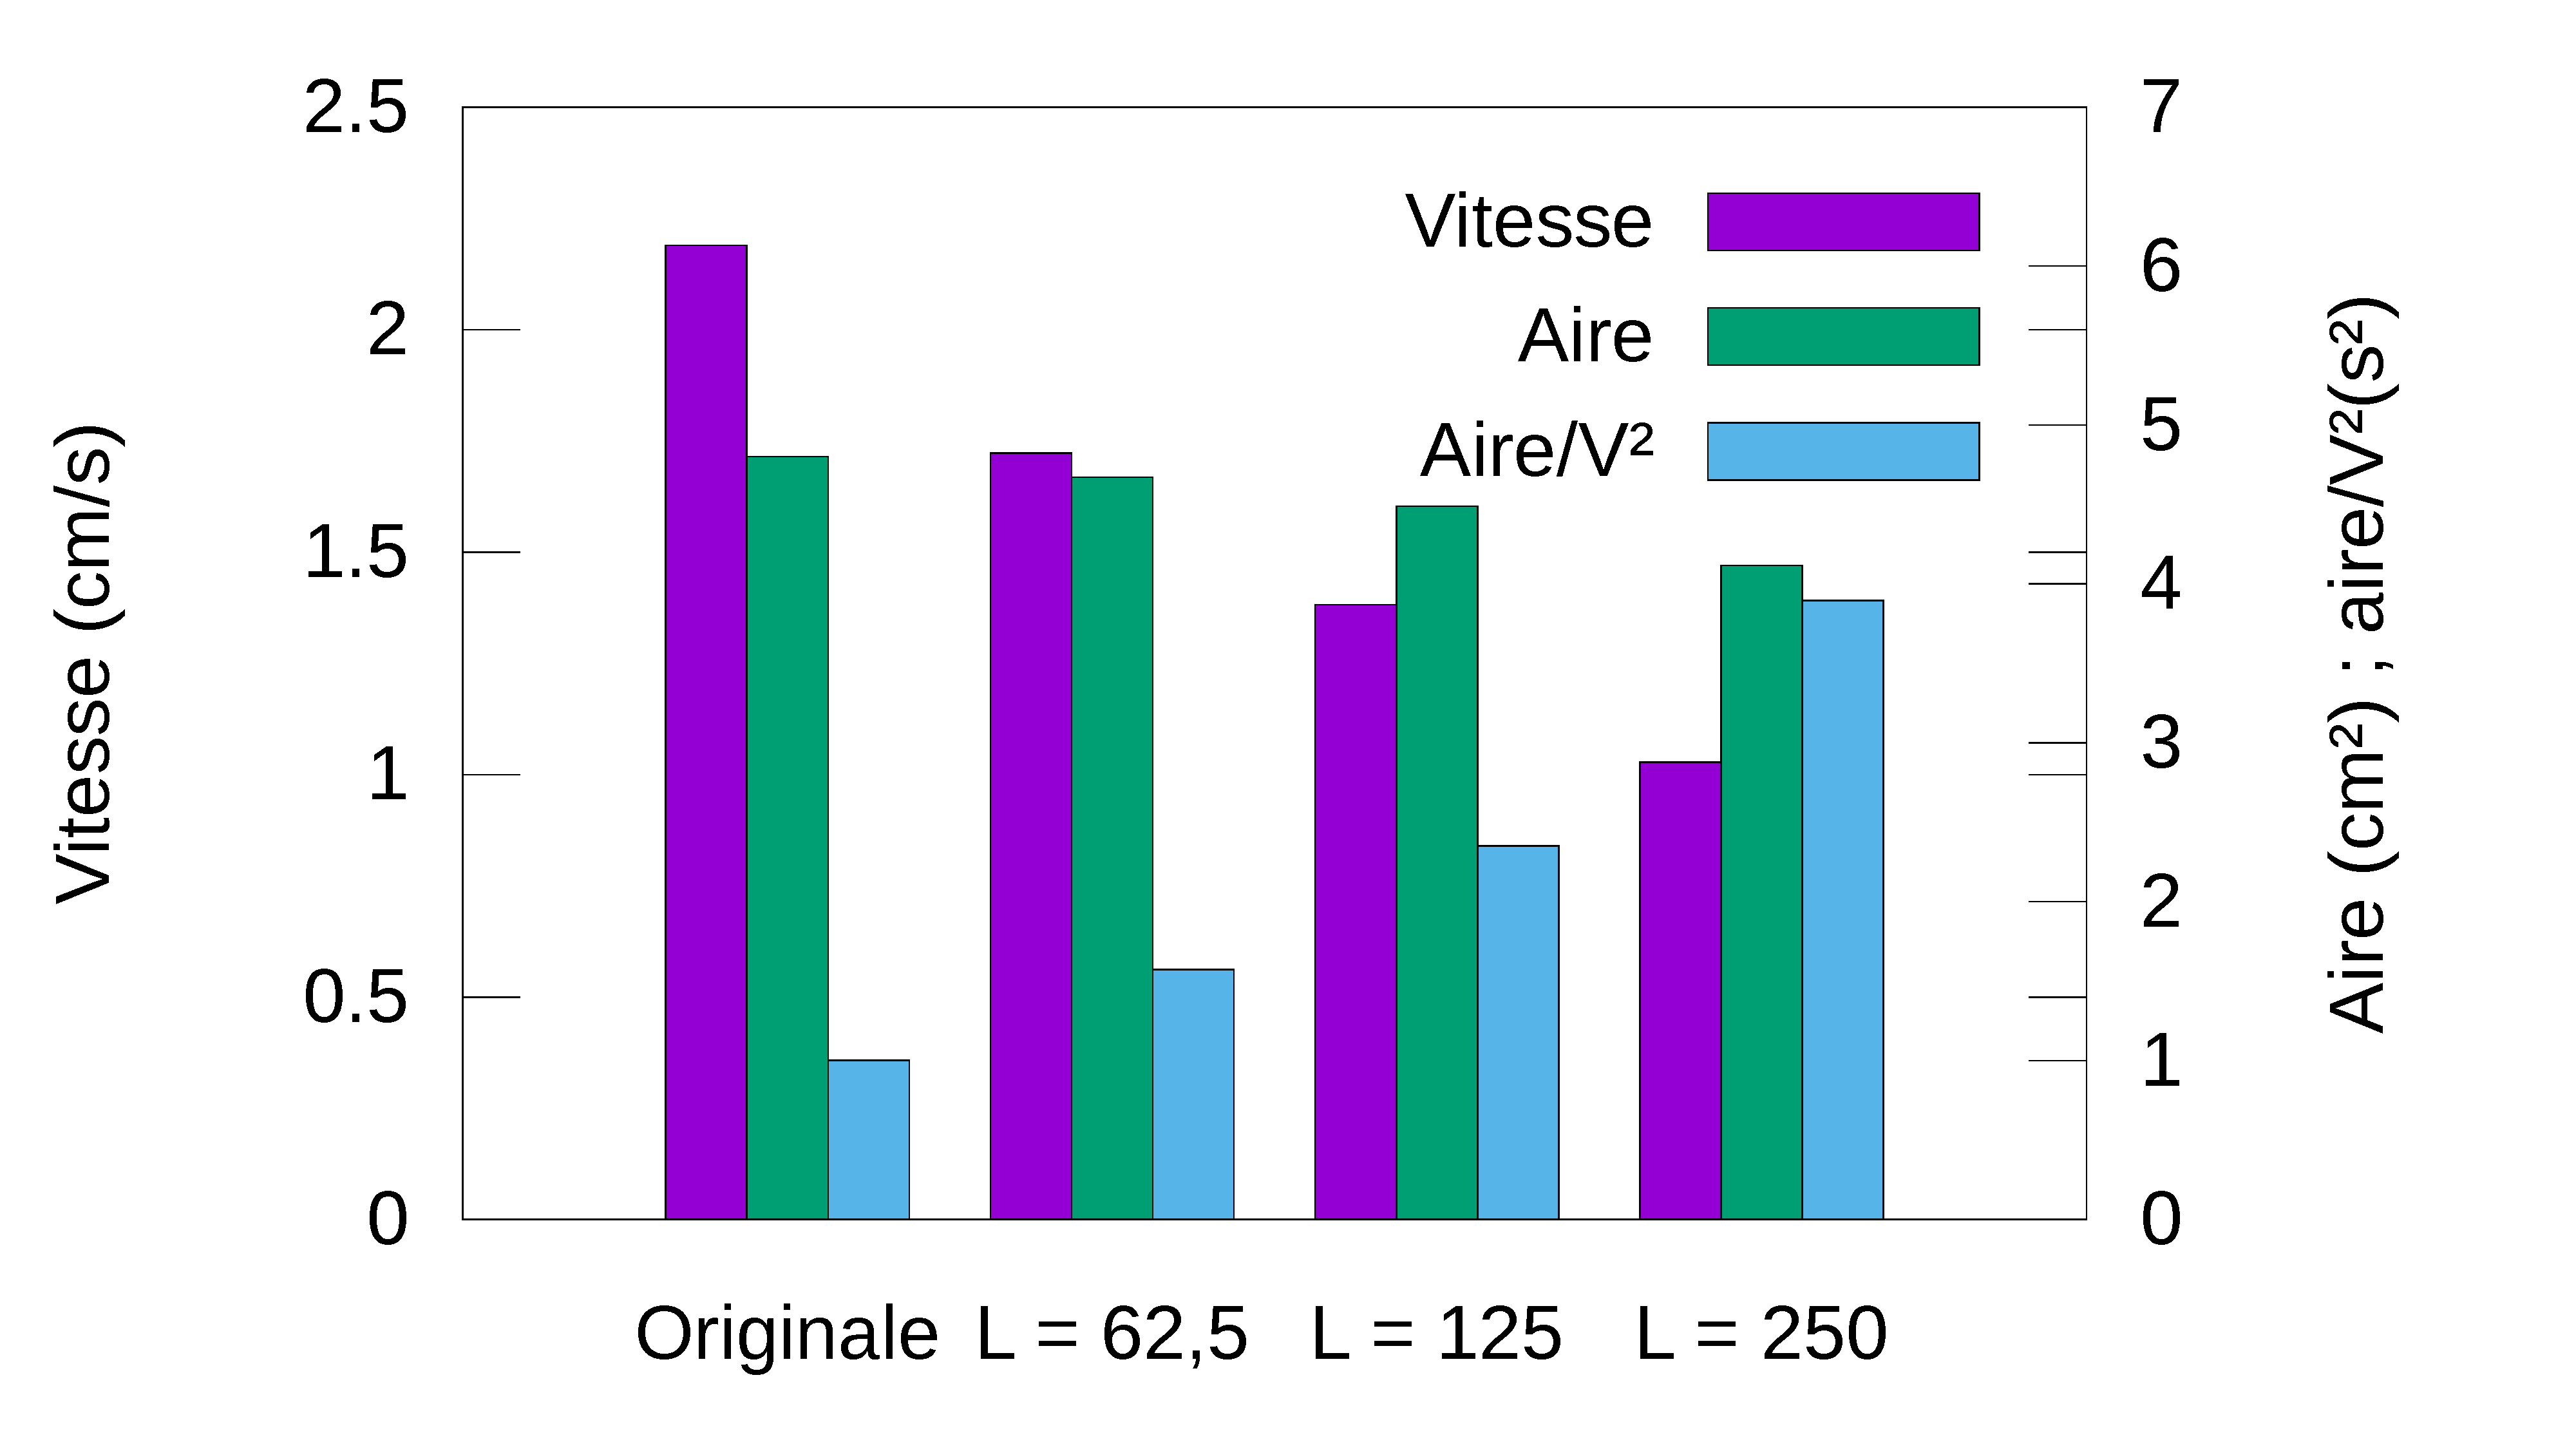
\includegraphics[width=0.5\textwidth]{figures/ch5/filteringByMovingAverageHistograms}
		\caption[Effet du filtrage par moyenne mobile]{Effet du filtrage par moyenne mobile sur les caractéristiques d'une trajectoire. Celle-ci, générée avec $V=2,19~cm/s$, $F=32~Hz$, et $A=120\degree{}$, se trouve modifiée de telle manière que la vitesse moyenne de la cible chute drastiquement --- de 2,19~cm/s à 1,03~cm/s lorsque la fenêtre mobile a une largeur de 250~ms. L'aire de l'enveloppe convexe demeure relativement stable.}
		\label{fig:filteringByMovingAverageHistograms}
	\end{figure}
	
	
	\subsection{Utilisation dynamique des proxies}
	\label{sub:dynamicProxies}
	Comme nous le précisions notamment dans la section~\ref{sub:techAug} qui évoque les techniques fondées sur l'augmentation des cibles, cette approche a l'inconvénient majeur d'accroître l'encombrement visuel, généralement d'un facteur deux lorsqu'elle implique l'utilisation de \emph{proxies}. Toutefois, il est tout à fait possible de mitiger cet impact en combinant cette approche avec de la prédiction intentionnelle. Par exemple, la technique \emph{Hook}~\cite{ortega2013hook} maintient en permanence une liste des N cibles potentielles les plus proches du curseur, où N est un entier naturel paramétrable. Ce procédé très simple pourrait être utilisé pour restreindre l'usage des \emph{proxies} : seules les N cibles en question en seraient accompagnées, les autres étant jugées trop loin du curseur pour être visées par l'utilisateur.
	
	Naturellement, selon le contexte, d'autres approches pourraient être pertinentes, comme celle d'\emph{IntenSelect}~\cite{de2005intenselect}, par exemple, fondée sur un principe similaire, mais appliqué à des rayons lancés depuis un périphérique de saisie, plutôt qu'à un curseur ponctuel. Quelle que soit l'approche exacte choisie, si le nombre de \emph{proxies} est beaucoup plus petit que le nombre total de cibles potentielles, l'encombrement visuel ajouté est faible, potentiellement inférieur à 10~\%{}, voire moins si l'on opte pour des \emph{proxies} partiellement transparents, par exemple.

	\subsection{Combinaison avec des techniques existantes}
	Les propositions détaillées ci-dessus portent sur le comportement des cibles, ou d'éventuels \emph{proxies} que l'on pourrait leur ajouter. Par conséquent, il est tout à fait possible de les combiner avec des techniques de sélection existantes, pour peu qu'elles ne consistent pas à modifier le comportement des cibles, ou du moins de le modifier de manière incompatible avec nos propositions.
	
	Les techniques fondées sur un curseur zonal ou du lancer de rayon (notamment avec désambiguïsation) peuvent être combinées avec nos propositions. Il en va de même de la sélection en cascade, ou de la prédiction de la trajectoire du curseur.
	
	Les techniques de manipulation du temps sont moins appropriées à de telles combinaisons, mais l'augmentation des objets est parfaitement possible, de même que la prédiction intentionnelle, que l'on appliquera aux seuls \emph{proxies} plutôt qu'à leurs cibles-mères.
	
	Nous recommandons donc de se rapporter à notre taxinomie des techniques de sélection (chapitre~\ref{chap2}) afin de choisir la plus approprié à chaque contexte applicatif, et de faire de même avec l'ensemble des propositions que nous détaillons dans le chapitre présent (section~\ref{sub:vfaGuide}) afin de choisir la meilleure combinaison possible. Nous suggérons par exemple de combiner le filtrage fréquentiel, qui conserve bien l'allure d'une trajectoire et son enveloppe convexe, avec la technique \emph{Hook}~\cite{ortega2013hook}, qui a fait ses preuves, mais n'est pas conçue pour gérer le mouvement brownien, que le filtrage fréquentiel permet, dans une certaine mesure, \og d'ordonner \fg{}.

\section{Estimer la difficulté de sélection pour mieux la réduire}
	Cependant, il n'est pas toujours possible de modifier le comportement des cibles. Même l'ajout de \emph{proxies} peut poser problème, y compris en en limitant le nombre par des heuristiques intentionnelles. Ces conditions ne rendent pas le modèle VFA inutile pour autant. D'une part, il permet d'estimer la difficulté de la tâche, et peut donc informer la conception de l'interface d'une application en indiquant si une aide à la sélection est nécessaire, si le nombre d'objets doit être réduit, si les objets doivent être agrandis, etc. D'autre part et surtout, il est peut-être possible d'utiliser les informations qu'il fournit pour réduire la difficulté moyenne d'une tâche de sélection.
	
	En effet, dans la plupart des contextes applicatifs évoqués au cours du chapitre~\ref{chap1}, les cibles potentielles forment un ensemble hétérogène du point de vue cinématique, c'est-à-dire que leurs mouvements respectifs ne sont pas tous de même nature. En particulier, les paramètres VFA qui les décrivent ne sont pas les mêmes.
	
	\subsection{Différents parmètres VFA, différentes difficultés}
	De fait, dans un contexte hétérogène particulier, la difficulté inhérente à la sélection d'une cible donnée n'est pas forcément la même que pour une autre cible. Or, les paramètres VFA, qui permettent d'estimer cette difficulté (notamment par le truchement de l'espérance de l'aire de l'enveloppe convexe associée, voir la figure~\ref{fig:perf_V_RealArea_better_fit} de la section~\ref{sub:areaVperf}) sont de fait différents d'une cible à l'autre, et peuvent être déterminés. Selon le contexte, ils seront déterminés exactement, ou estimés, ou mesurés en temps réel, mais ils peuvent presque toujours être connus.
	
	Il est donc possible de dresser un tableau des différentes cibles (ou des différents types de cibles) et de leurs difficultés de sélection respective, afin de savoir quels objets poseront le plus de problèmes aux utilisateurs.
	
	\subsection{Distance de Fitts et cibles mobiles}
	\label{sub:fittsDistance}
	Nous avons déjà vu que le modèle de Fitts pur n'était pas adapté à la sélection de cibles mobiles, et que des versions modifiées de ce modèle y étaient parfois préférées --- voir la section~\ref{sub:fittsMobile}. Ces modèles intègrent toujours la distance entre le curseur et la cible (que nous appelons ici distance de Fitts) comme facteur. Cependant, nos observations précédentes ont montré que lorsque les mouvements d'une cible sont vifs et imprévisibles, la phase de la tâche de sélection consistant à s'approcher de la cible est dominée par la phase consistant à la saisir une fois que l'on en est proche. De fait, il est possible que, dans ces cas-là, le temps de sélection soit peu dépendant de la distance de Fitts.
	
	% 1.0f = 2.84 cm sur 22 pouces
	% Donc environ 1.94 cm sur 15 pouces
	Pour évaluer cette hypothèse, nous avons mené une petite étude sur 8 sujets, 6 hommes et 2 femmes, âgés de 22, 23, 23, 28, 22, 29, 26 et 26 ans, respectivement, et tous droitiers. Nous avons utilisé un protocole identique à celui décrit dans la section~\ref{sub:as_protocol}, mais avec un écran de 15 pouces de diagonale, et une seule combinaison VFA : V = 31,25~\%{} de la largeur du cadre par seconde, soit 9,68~cm/s, F = 20~Hz, et A = 100\textdegree{}. Cette condition fut choisie pour sa difficulté. Chaque sujet a effectué 42 sélections pour chacune des trois distances de Fitts évaluées : 12,5~\%{}, 25~\%{}, et 50~\%{} de la largeur du cadre, soit environ 3,87~cm, 7,75~cm, et 15,49~cm.
	
	\subsubsection{Temps de sélection et erreurs}
	Nous présentons les résultats obtenus sur la figure~\ref{fig:fittsDistAndPerf}, sous forme de moyennes et d'intervalles de confiance à 95~\%{}. Les temps de sélection moyens bruts sont sur la figure~\ref{fig:ampTimeRes}, les moyennes des temps de sélection normalisés sont sur la figure~\ref{fig:normTimes}, les moyennes des taux d'erreurs normalisés sont sur la figure~\ref{fig:normErrors}, et les moyennes des produits $Temps\times(Erreurs+1)$ sont sur la figure~\ref{fig:normProducts} --- cette dernière métrique est détaillée dans la section~\ref{sub:product}. Comme nous le supposions, la distance de Fitts ne semble plus avoir d'influence majeure sur les performances de sélection d'une cible mobile lorsque la difficulté est suffisamment élevée. Il n'en va cependant pas de même de la largeur de la cible, comme nous le verrons plus loin.

	\begin{figure}[!htb]
		%\centering
		\begin{subfigure}[t]{0.49\textwidth}
			\centering
			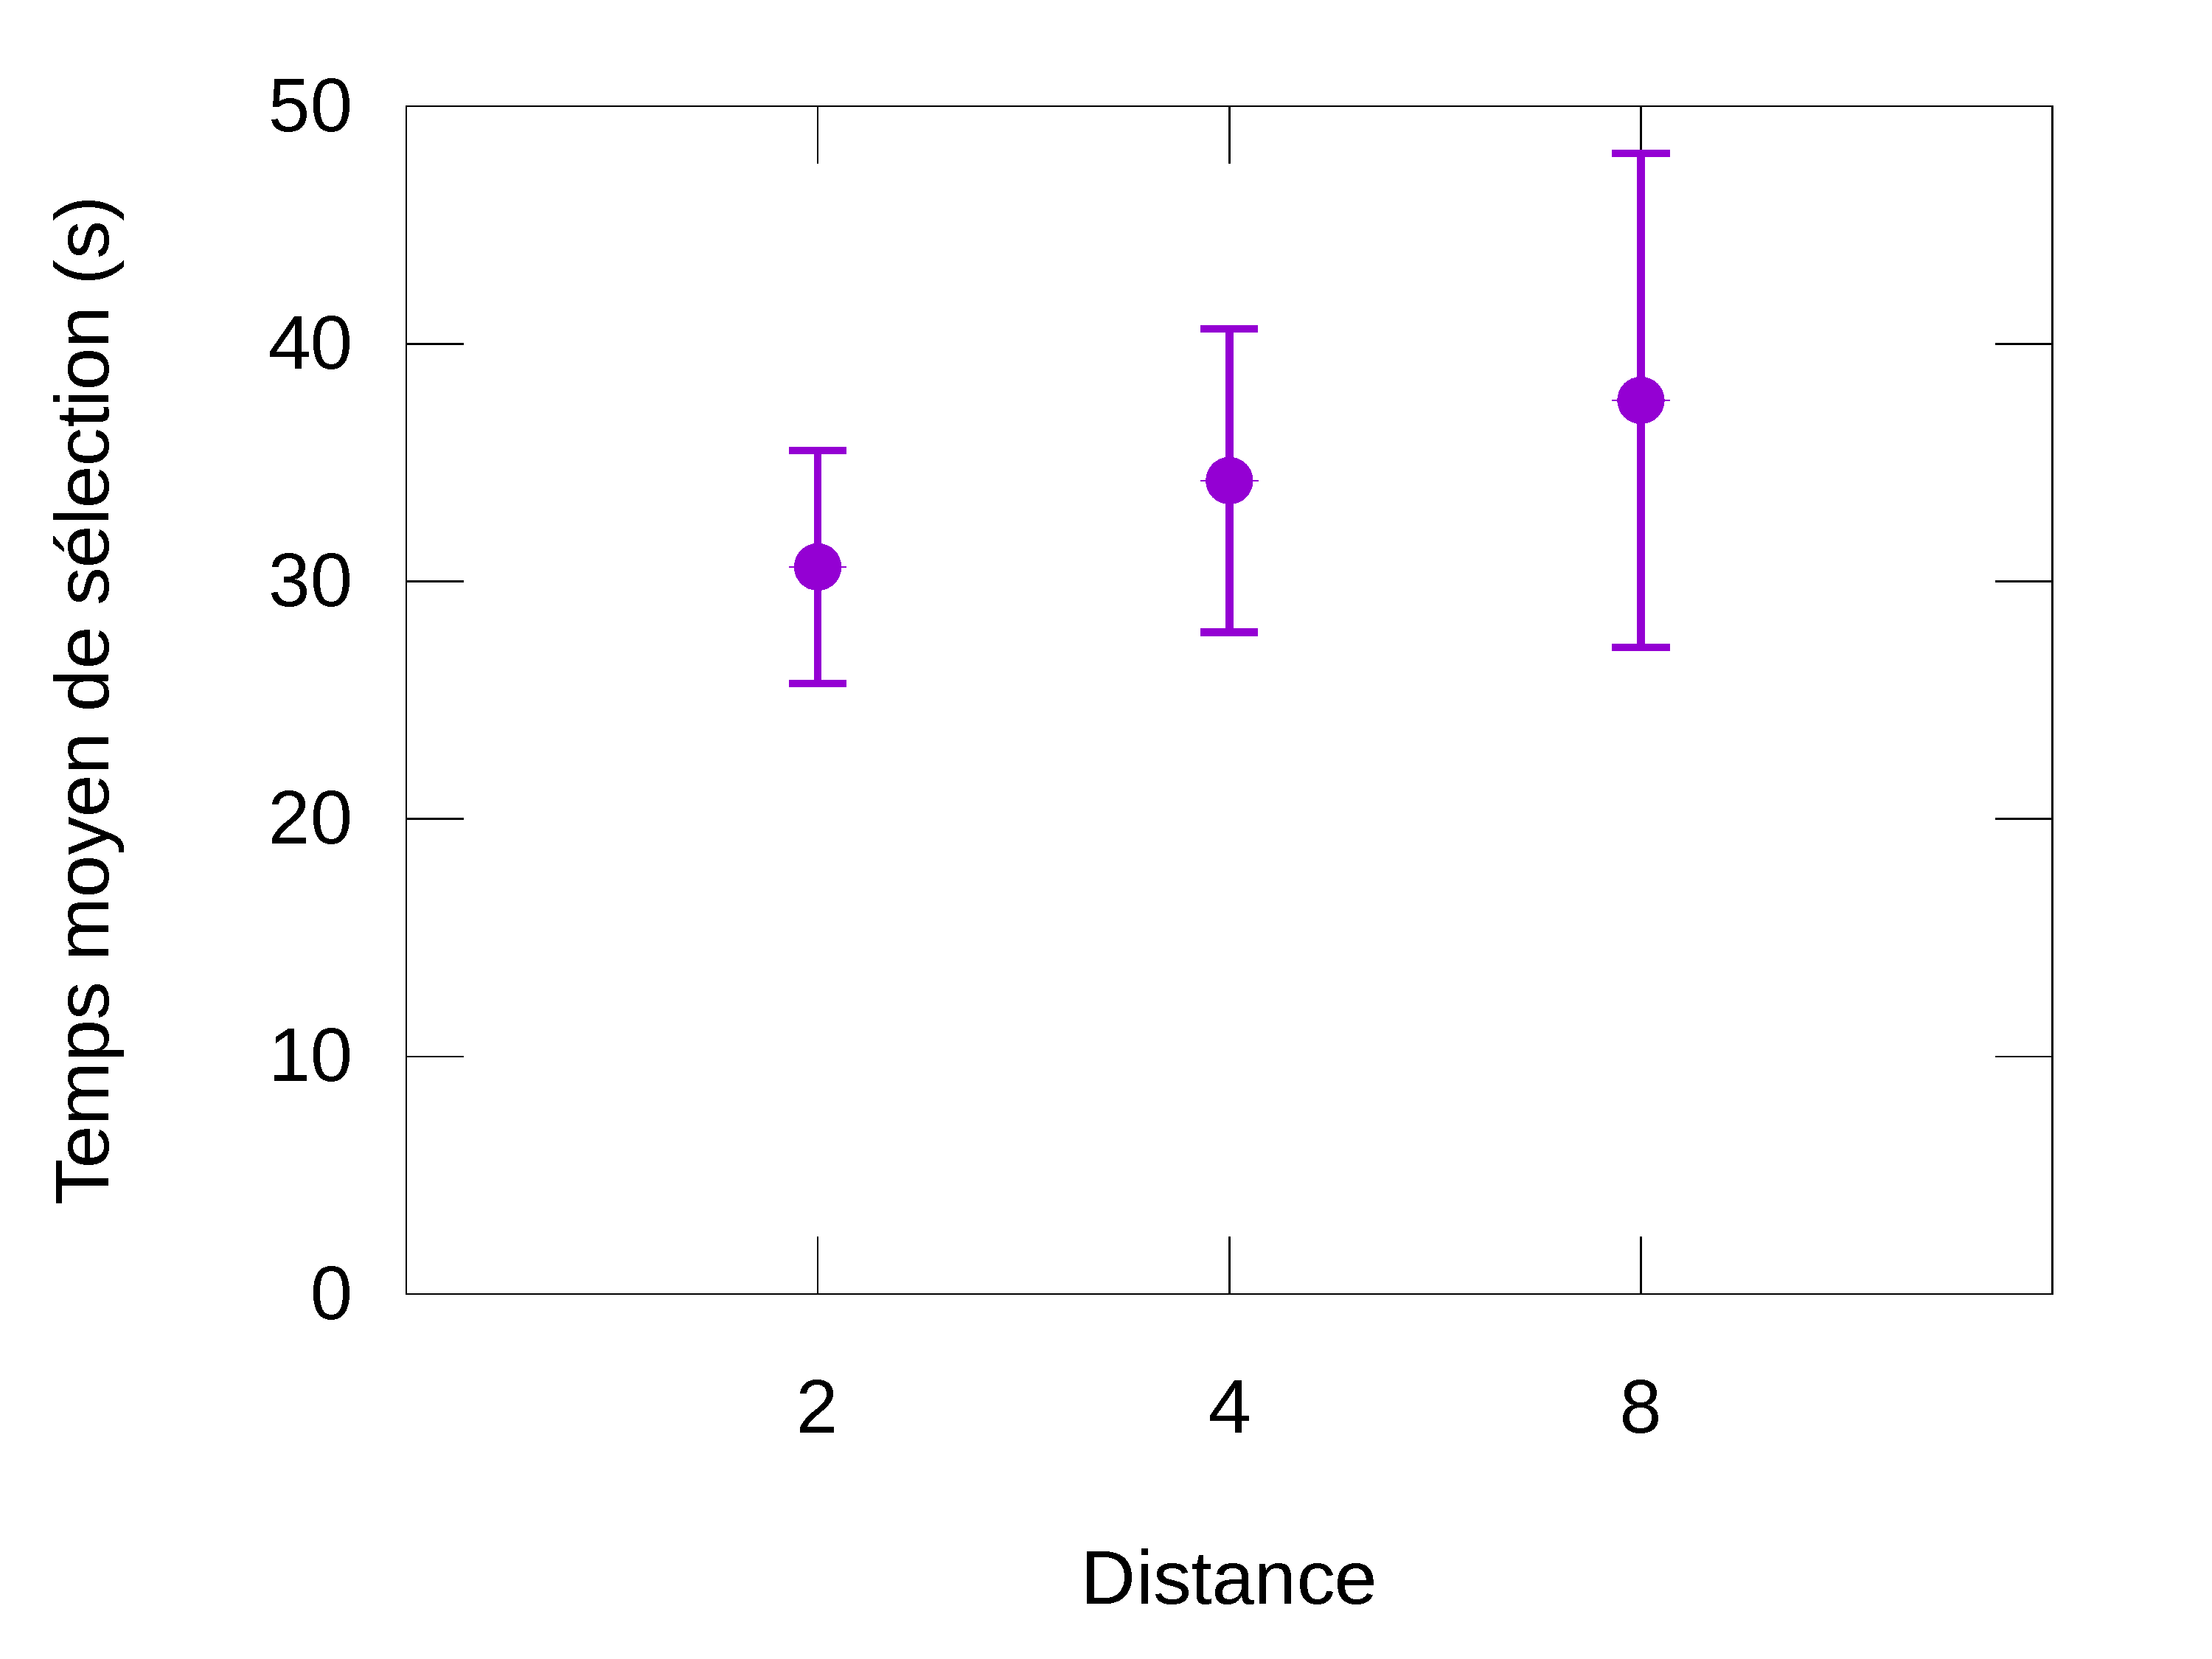
\includegraphics[width=\textwidth]{figures/ch5/ampTimeRes}
			\caption{Temps de sélection bruts.}
			\label{fig:ampTimeRes}
		\end{subfigure}
		~
		\begin{subfigure}[t]{0.49\textwidth}
			\centering
			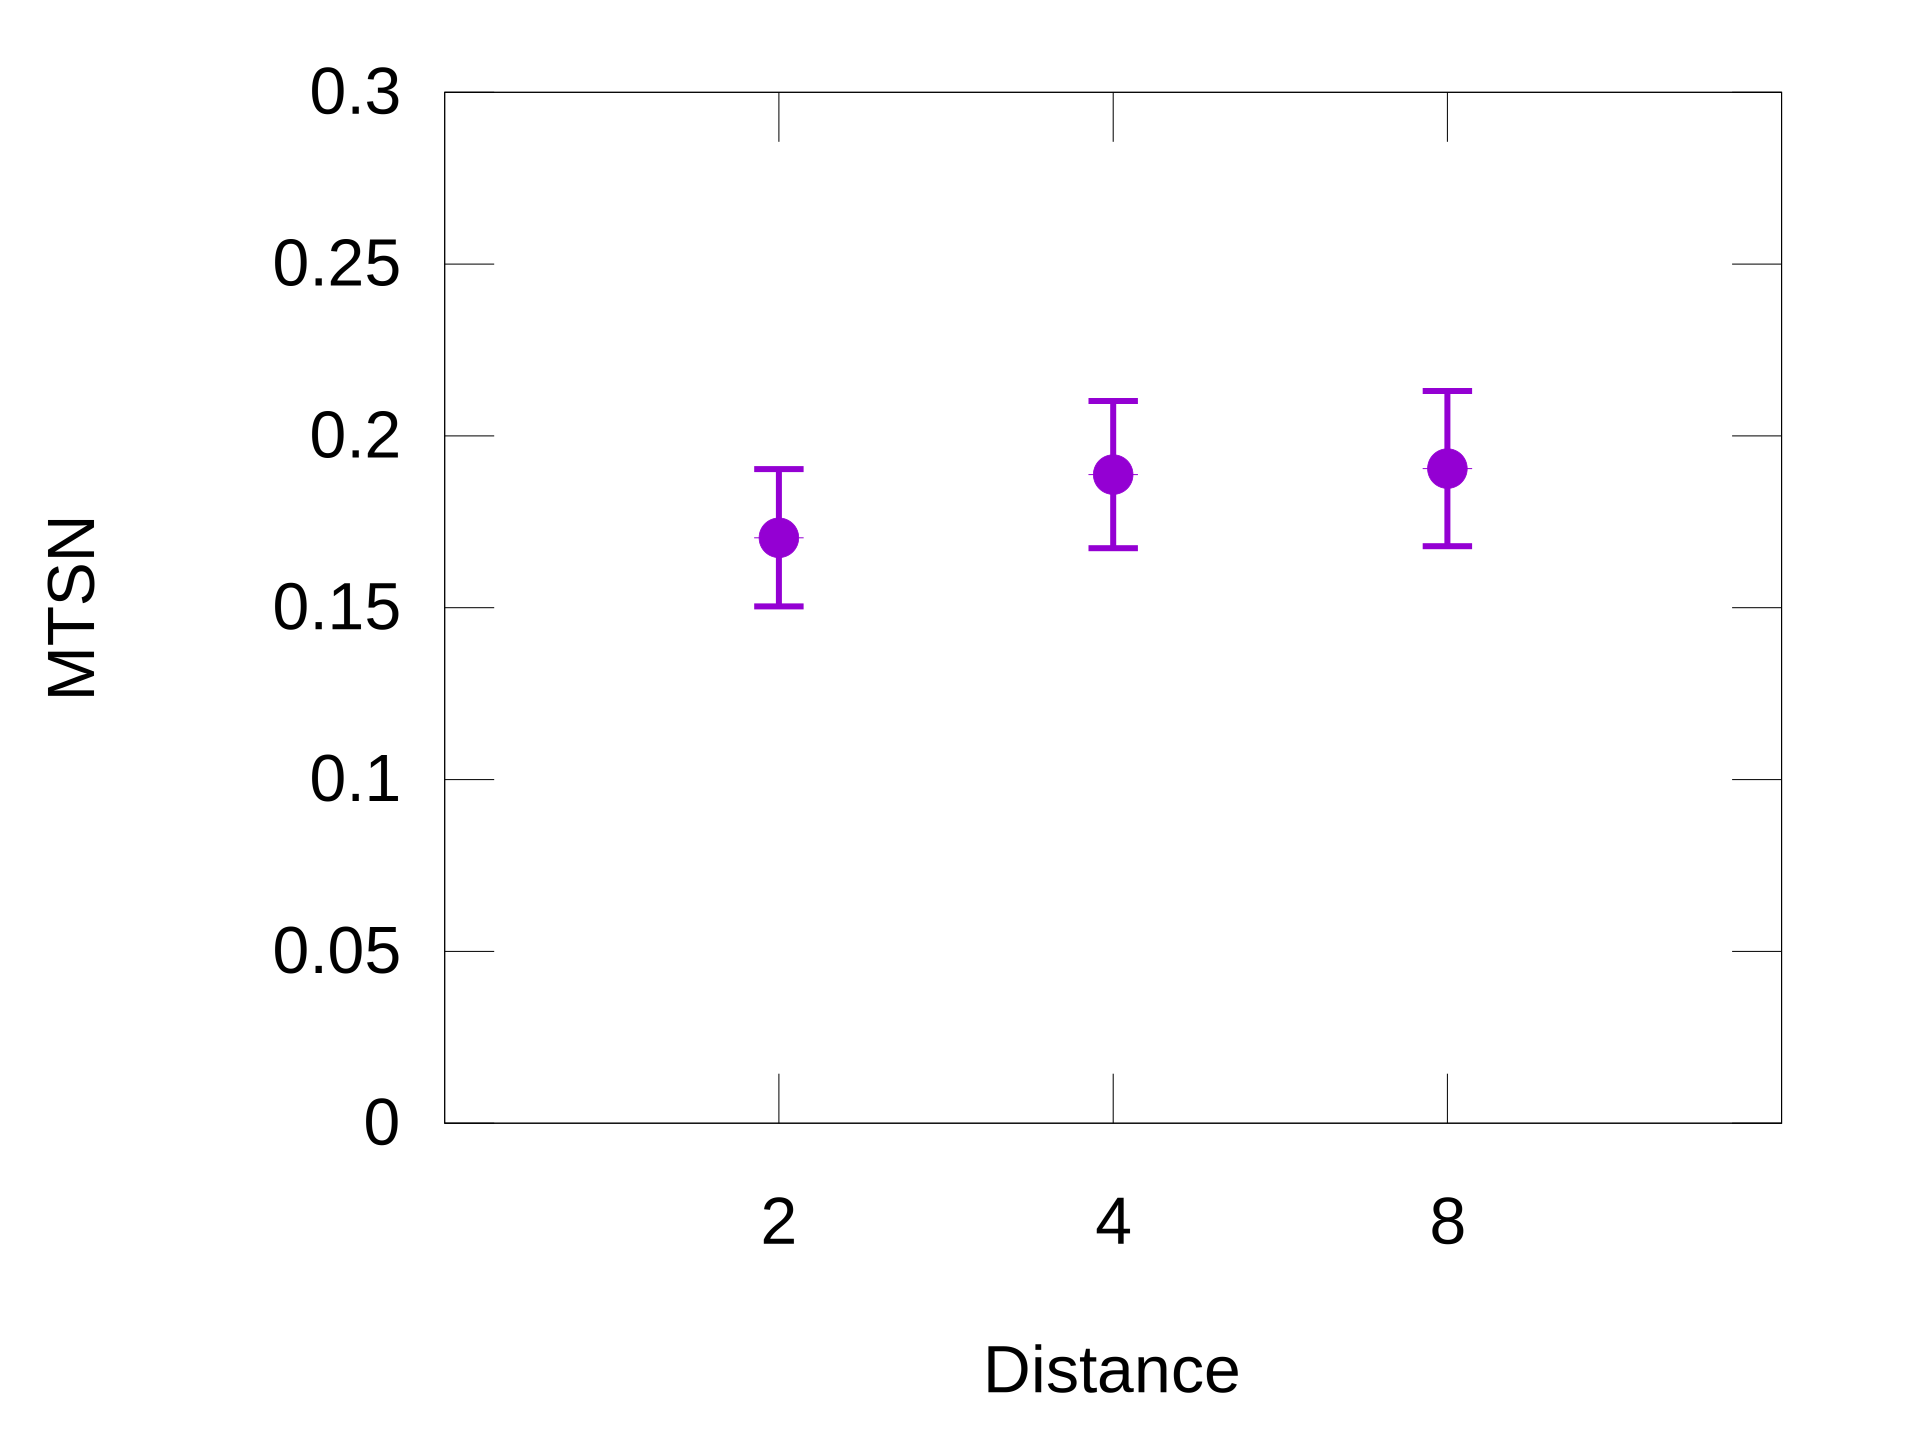
\includegraphics[width=\textwidth]{figures/ch5/normTimes}
			\caption{Moyenne des temps de sélection normalisés.}
			\label{fig:normTimes}
		\end{subfigure}
		~
		\begin{subfigure}[t]{0.49\textwidth}
			\centering
			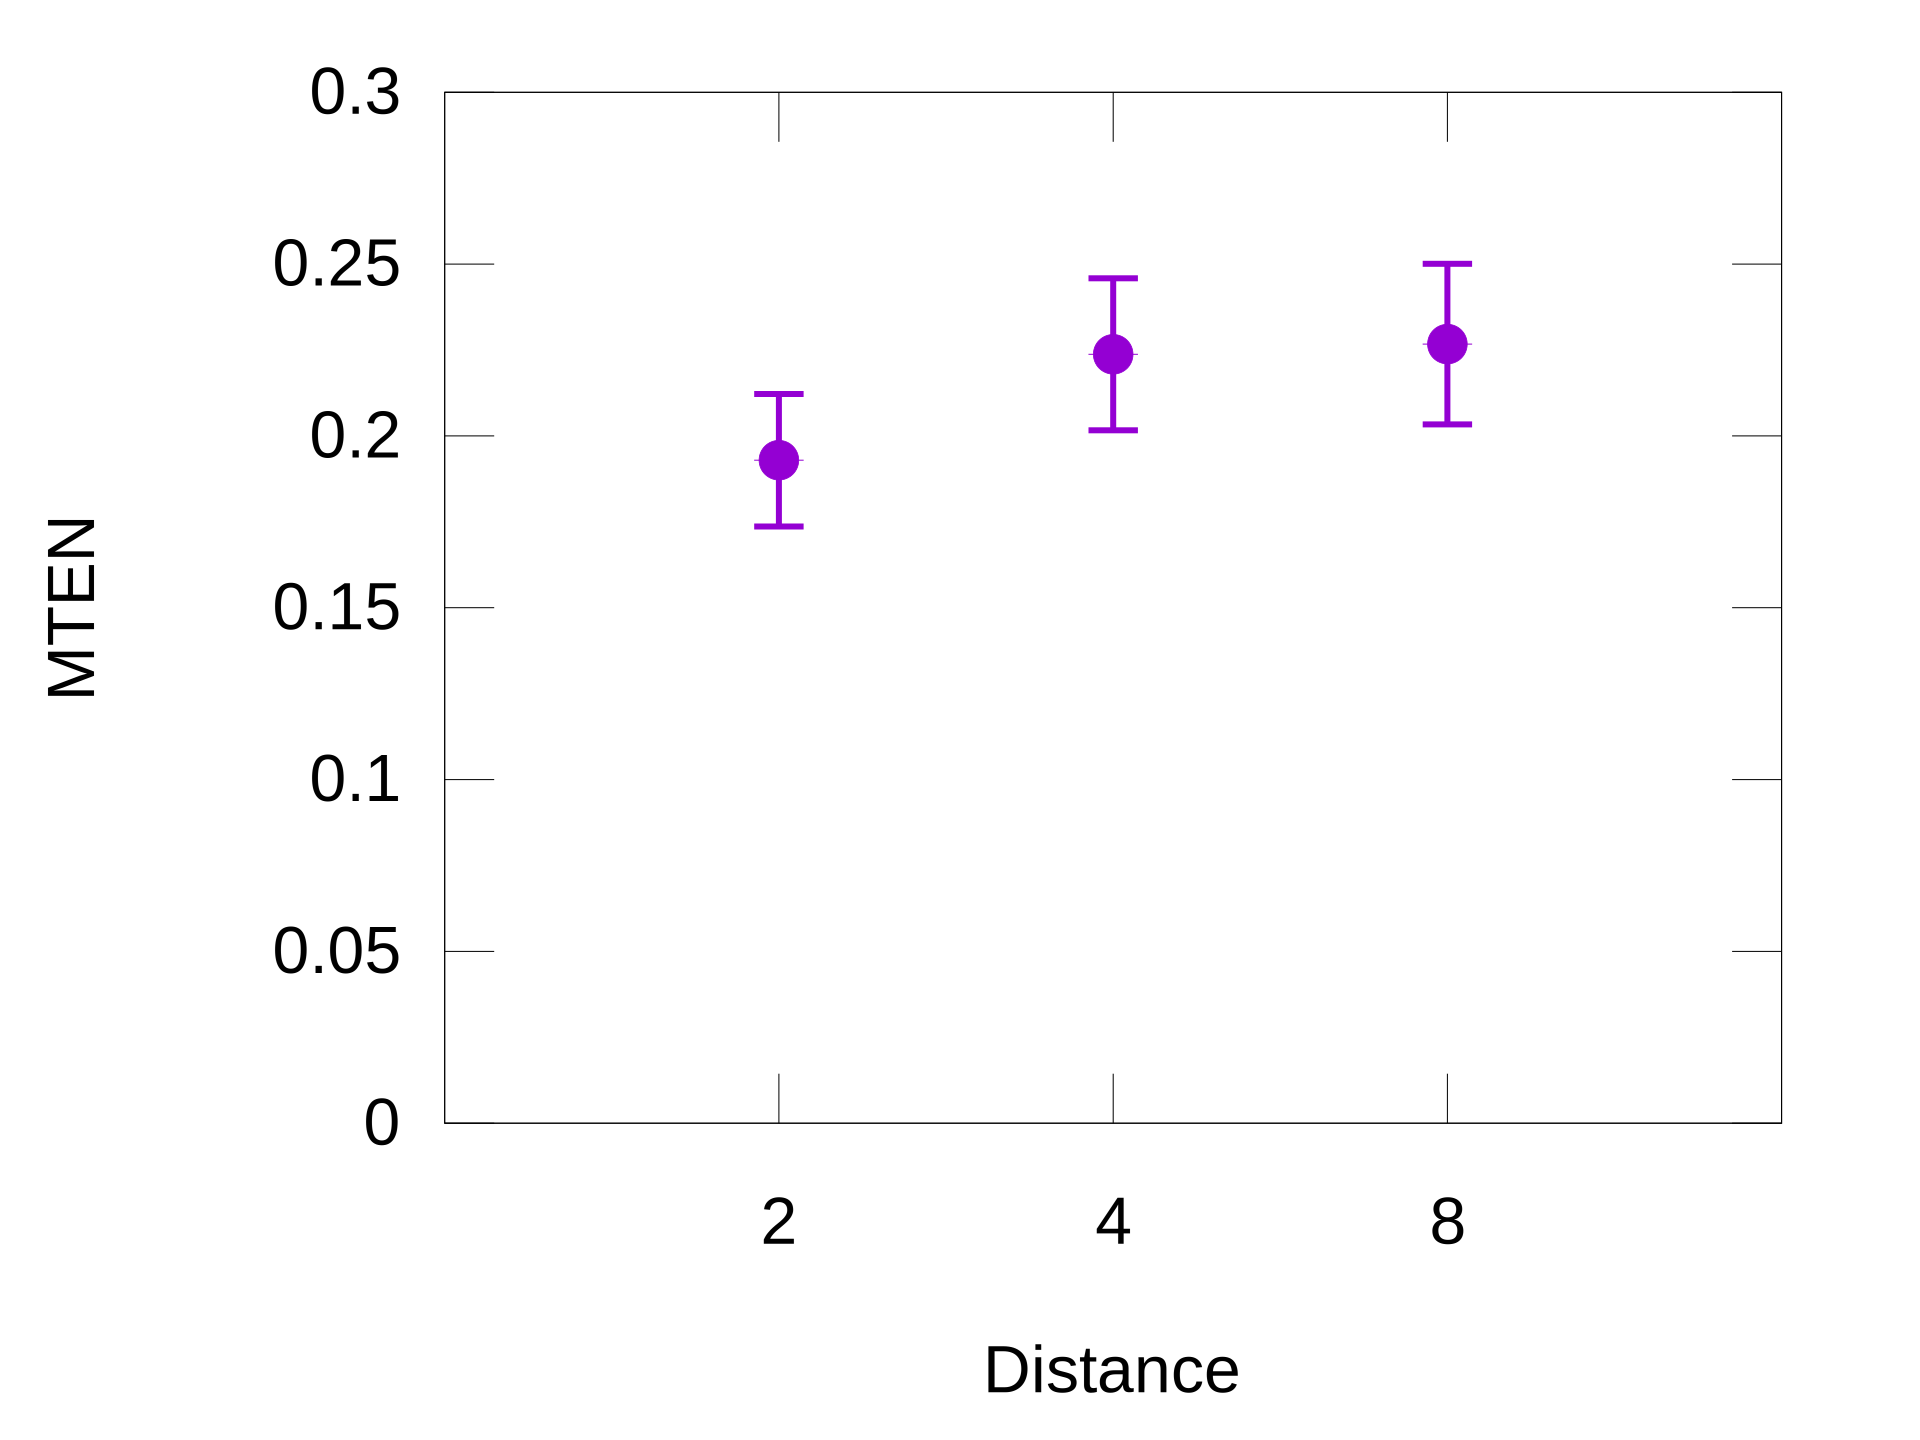
\includegraphics[width=\textwidth]{figures/ch5/normErrors}
			\caption{Moyenne des taux d'erreurs normalisés.}
			\label{fig:normErrors}
		\end{subfigure}		
		~
		\begin{subfigure}[t]{0.49\textwidth}
			\centering
			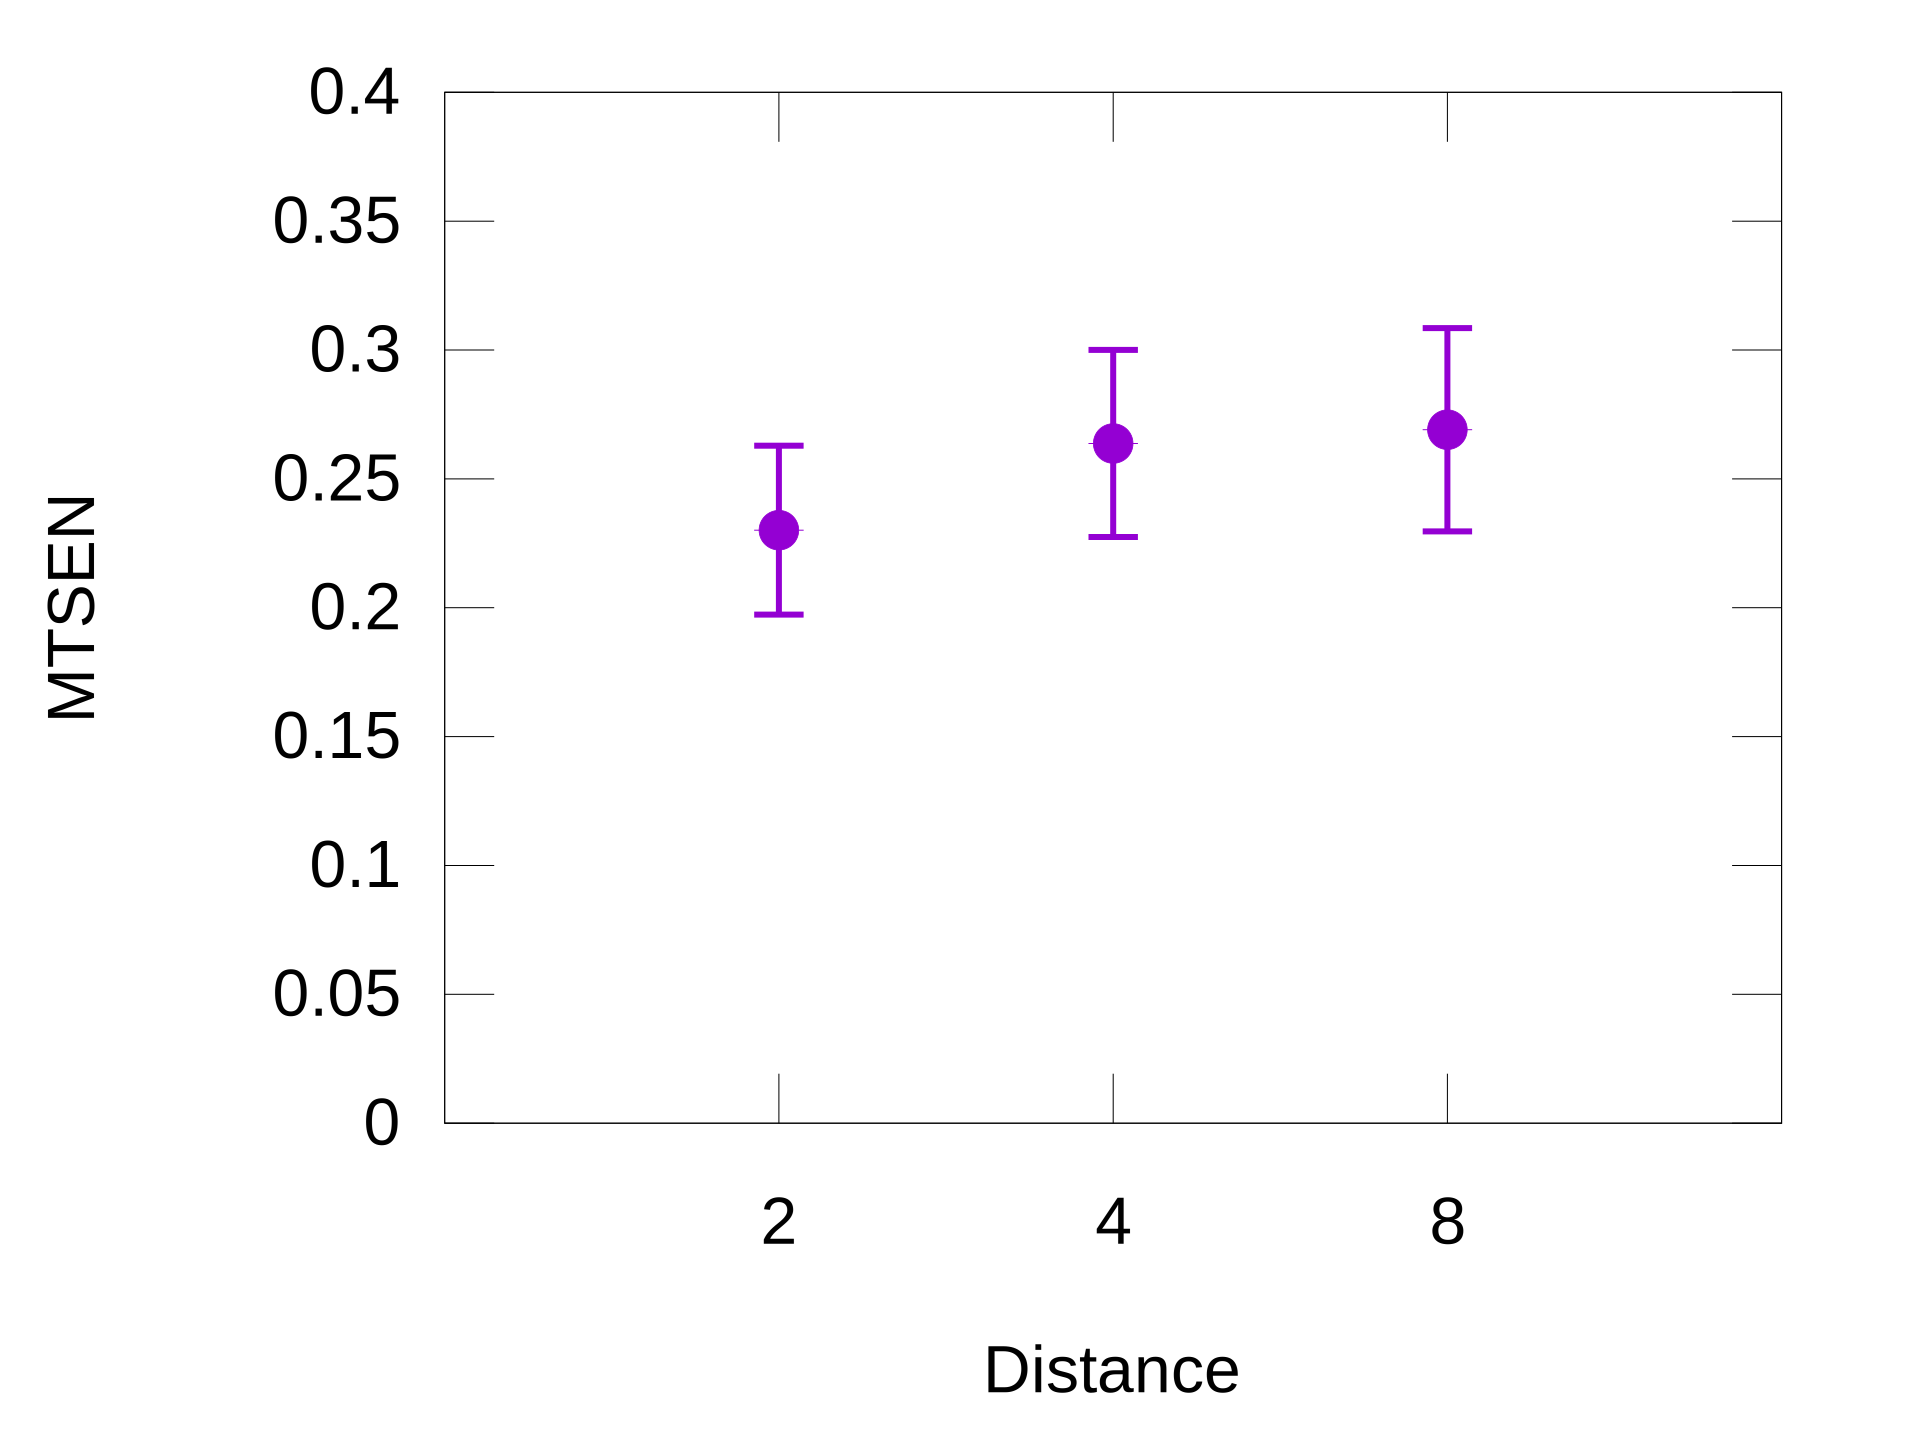
\includegraphics[width=\textwidth]{figures/ch5/normProducts}
			\caption{Moyenne des performances sur E et T normalisés.}
			\label{fig:normProducts}
		\end{subfigure}
		\caption[Distance de Fitts et performances de sélection]{Distance de Fitts et performances de sélection.}
		\label{fig:fittsDistAndPerf}
	\end{figure}

	
	\subsection{Espace d'affichage et encombrement visuel}
	Bien que nous n'ayons pas spécifiquement étudié ce paramètre au cours de l'étude que nous présentons dans les section~\ref{sub:interact} et suivantes~\cite{kouyoumdjian2015characterizing}, la largeur de Fitts demeure très importante dans une tâche de sélection de cible mobile, ce qu'illustrent par ailleurs les modèles d'autres auteurs, présentés dans la section~\ref{sub:fittsMobile}. Par conséquent, augmenter la taille d'une cible mobile en facilite toujours la sélection, et des techniques conçues spécifiquement pour cette tâche sont fondées sur ce principe. C'est notamment le cas de \emph{Comet}, dont les auteurs ont confirmé l'apport empiriquement~\cite{hasan2011comet}. Il en est de même pour \emph{AttachedShock}~\cite{you2012attachedshock, you2014attachedshock}.
	
	Mais ces dernières ont l'inconvénient d'augmenter l'encombrement visuel global de la scène. Certes, il serait probablement possible d'utiliser une heuristique intentionnelle pour mitiger ce problème, comme nous le proposions pour les \emph{proxies} dans la section~\ref{sub:dynamicProxies}, en n'augmentant que les objets dont on estime qu'ils peuvent être visés par l'utilisateur. Mais l'on peut craindre que les changements de taille permanents des objets de la scène ne perturbent l'utilisateur, et nuisent au confort d'utilisation global.
	
	Plutôt que d'utiliser une heuristique intentionnelle pour choisir quelles cibles augmenter, il est possible de s'appuyer sur une estimation de la difficulté de sélection de chaque cible. Ainsi, il est possible de consacrer plus d'espace d'affichage aux objets mobiles en ayant le plus besoin. Nous avançons en effet que, dans le cadre de l'utilisation d'une technique d'augmentation des objets, il est pertinent de considérer l'espace d'affichage comme un budget, qu'il appartient au concepteur de l'application de répartir judicieusement. Il paraît logique, au moins intuitivement, d'allouer une plus grande proportion de cet espace aux cibles les plus difficiles à saisir. Plus formellement, nous émettons les hypothèses suivantes :
	
	\begin{description}
		\item[H1 :] Notre estimation de la difficulté de sélection d'une cible est plus fiable que l'usage des paramètres V, F, ou A.
		\item[H2 :] Si les cibles jugées difficiles sont agrandies, et les cibles jugées faciles sont rétrécies, de sorte que l'espace d'affichage alloué à l'ensemble des cibles demeure constant, les performances de sélection mesurées sur l'ensemble des cibles sont meilleures.
	\end{description}
	
	Ici, une cible \og jugée difficile \fg{} est une cible pour laquelle notre modèle prédit un temps de sélection relativement élevé, tandis qu'une cible \og jugée facile \fg{} a un temps de sélection prédit relativement faible (voir la figure~\ref{fig:perf_V_RealArea_better_fit} de la section~\ref{sub:areaVperf}).
	
	\subsection{Expérience et protocole}
	\label{sub:as_protocol}
	Afin d'évaluer notre hypothèse H1, nous avons mené une étude empirique avec 16 sujets, au cours de laquelle il leur était demandé de sélectionner des cibles rondes en cliquant dessus, dans un environnement homogène d'une part, et hétérogène de l'autre --- c'est-à-dire avec des cibles mues par les mêmes paramètres VFA et, respectivement, par des paramètres différents. Dans la condition hétérogène, chaque cible est de même taille ; dans la condition hétérogène, elles sont de tailles différentes selon l'estimation de leur difficulté de sélection, faite à partir de leurs paramètres VFA.
	
	\subsection{Dispositif expérimental et sujets}
	Chaque sujet ayant participé à l'étude l'a fait avec une machine identique : un ordinateur de bureau doté d'un écran de 22 pouces de diagonale (Dell E2210), et d'une souris optique filaire ambidextre (Logitech Premium Optical Mouse). Les sujets étaient assis sur des chaises de bureau, et avaient la possibilité d'ajuster la luminosité et le contraste de l'écran, selon leurs préférences personnelles, afin de garantir leur confort. Notre groupe de 16 sujets était constitué de 15 hommes et 1 femme, de 15 droitiers et 1 gaucher, son âge moyen est de 22 ans, avec un écart-type d'un peu plus de 4 ans.
	
	\subsection{Tâche et conditions}
	% 22 pouces -> environ 1,84 cm par 1.0f
	L'application utilisée pour mener l'étude affiche des disques en bleu sur un fond noir rectangulaire, de dimensions 45,44~cm~$\times$~25,56~cm, cerné d'un cadre gris. À tout moment, l'objet à sélectionner est rouge, tandis que les distracteurs demeurent bleus. Une fois que la cible est sélectionnée avec succès (c'est-à-dire une fois que le sujet a cliqué dessus), elle redevient bleue, et une autre devient rouge. Dans la condition homogène, chaque cible mesure 18,5~mm de diamètre (4,06~\%{} de la largeur du cadre).
	
	De surcroît, chaque nouvelle cible est repositionnée dès qu'elle devient rouge, à une distance par rapport au curseur précisément réglée sur 12,75~cm (28,125~\%{} de la largeur du cadre), dans une direction par rapport au curseur choisie de manière aléatoire, à une exception près : si la direction choisie implique une sortie du cadre noir servant de fond, une autre direction est choisie aléatoirement --- cette opération pouvant éventuellement être répétée plusieurs fois, jusqu'à ce qu'une position convenable soit trouvée. Ce déplacement soudain n'a été remarqué par aucun des sujets, sans doute parce qu'il a lieu à un moment où le sujet se concentre sur autre chose (la cible précédente qu'il vient de réussir à sélectionner) et parce que le changement de couleur, du bleu vers le rouge vif, fait distraction.
	
	La figure~\ref{fig:evalAppRunning} fournit des illustrations de l'application en cours d'exécution, dans sa condition homogène (figure~\ref{fig:homoRunning}), et dans sa condition hétérogène (figure~\ref{fig:heteroRunning}). Contrairement à la précédente étude, nous avons cherché à nous approcher des conditions d'une application \og réelle \fg{}, c'est-à-dire en plein écran. De fait, les dimensions et vitesses sont plus élevées, d'autant que nous avons souhaité nous concentrer sur les conditions les plus difficiles.
	
	\begin{figure}[!htb]
		\begin{subfigure}[t]{0.49\textwidth}
			\centering
			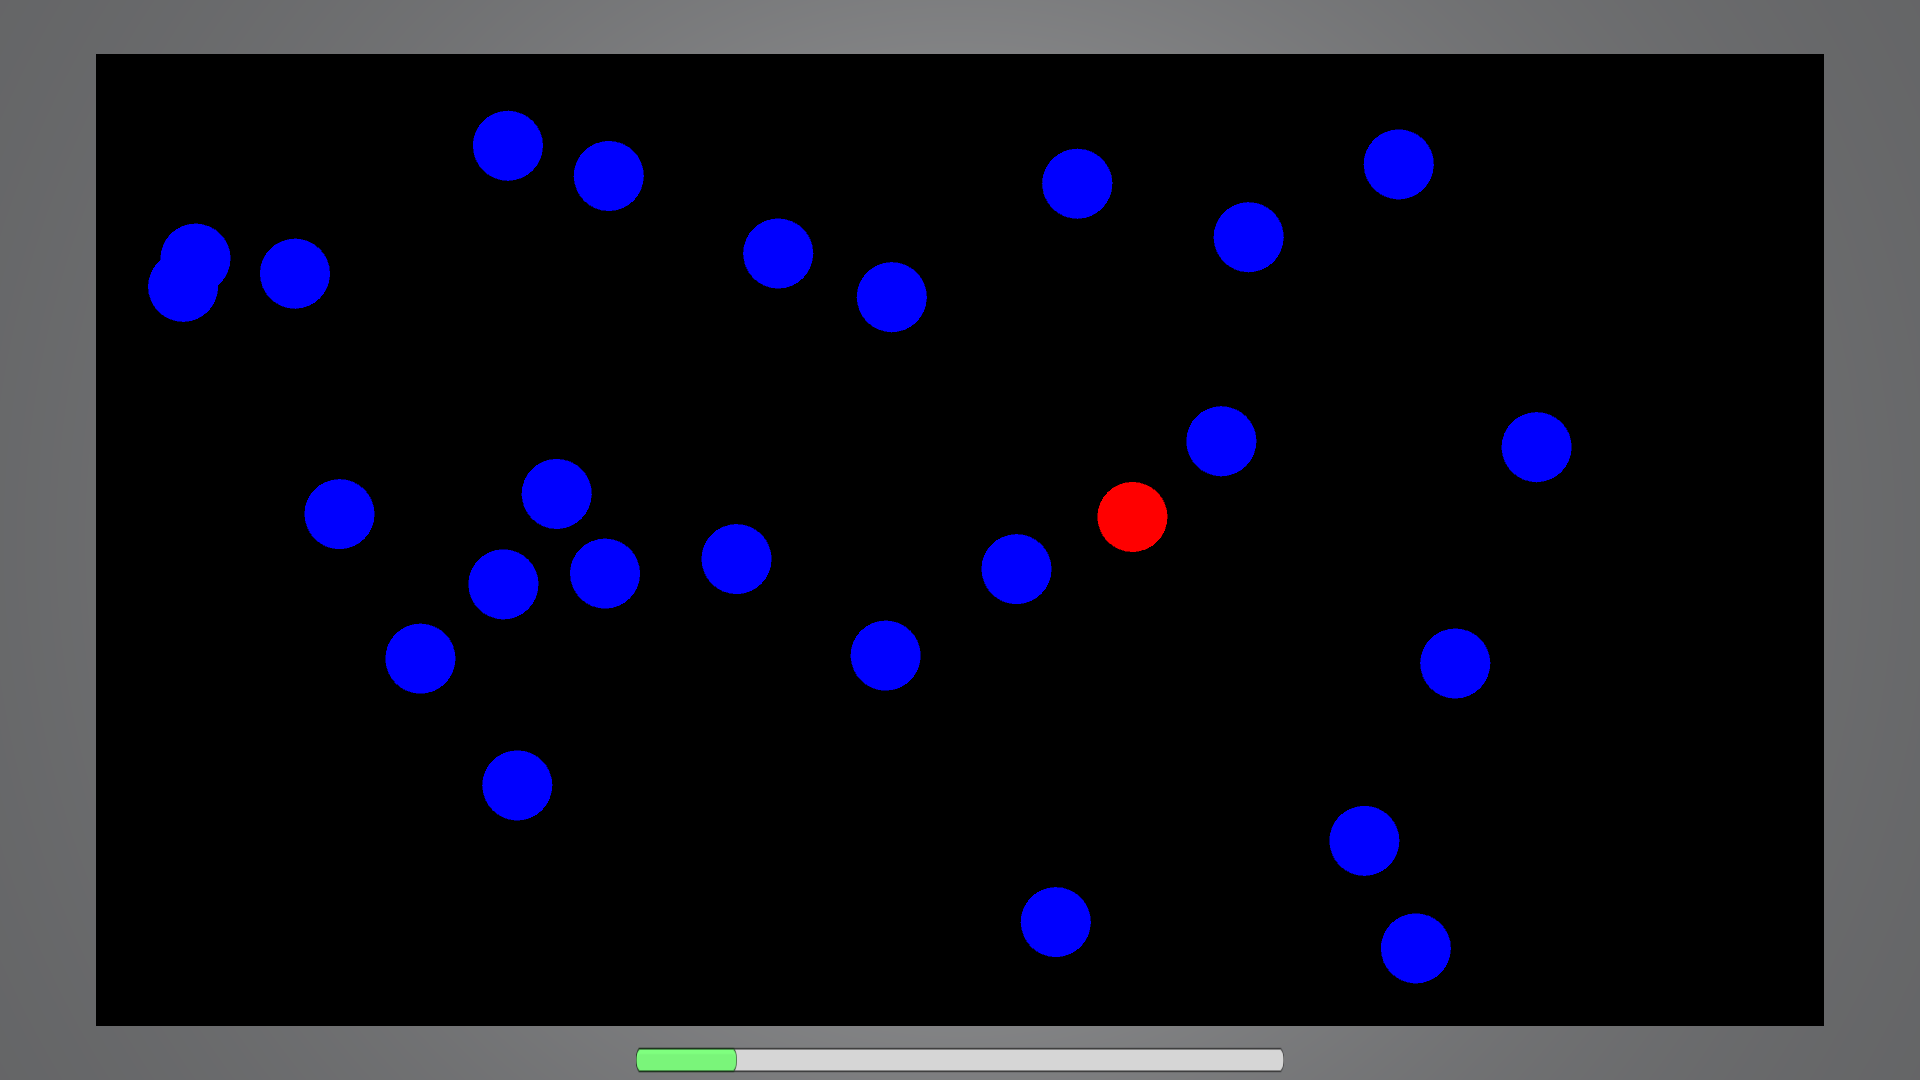
\includegraphics[width=\textwidth]{figures/ch5/homoRunning}
			\caption{Condition homogène : toutes les cibles font la même taille.}
			\label{fig:homoRunning}
		\end{subfigure}
		~
		\begin{subfigure}[t]{0.49\textwidth}
			\centering
			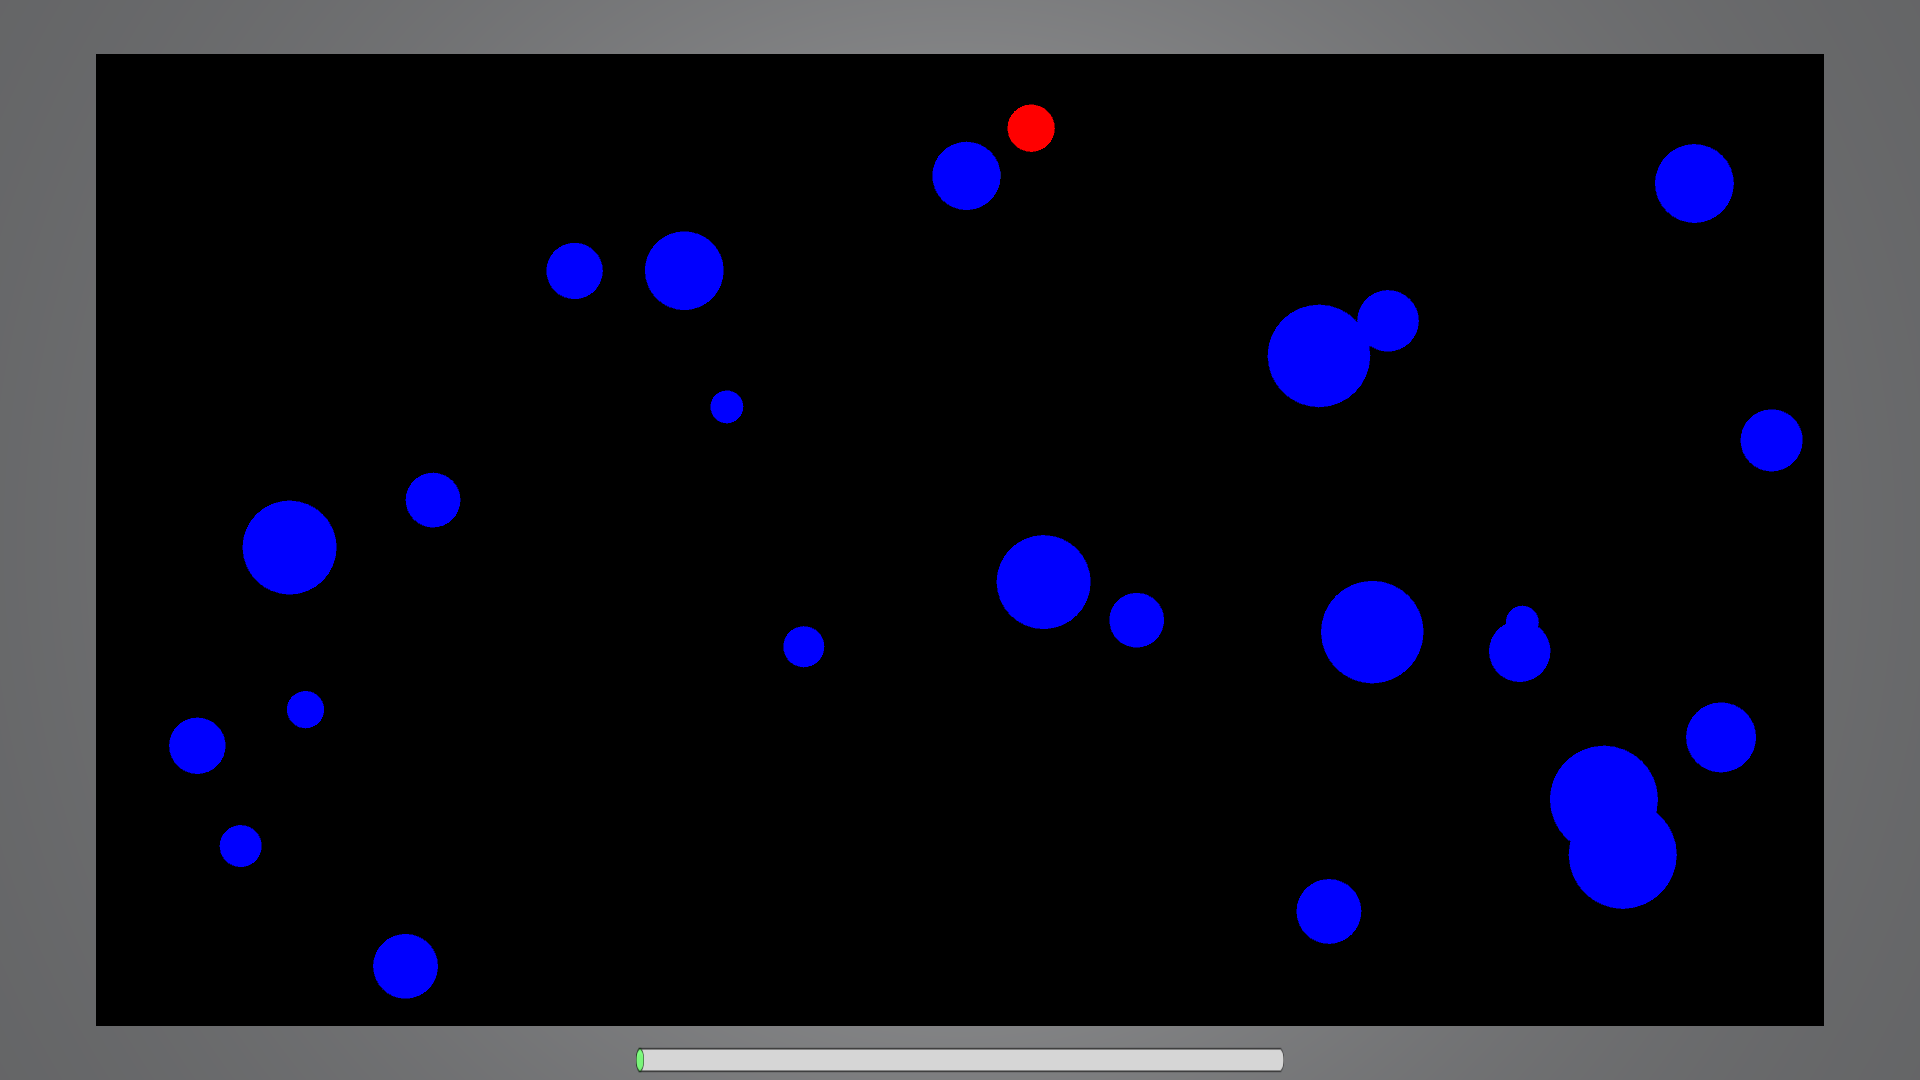
\includegraphics[width=\textwidth]{figures/ch5/heteroRunning}
			\caption{Condition hétérogène : les cibles sont de tailles différentes.}
			\label{fig:heteroRunning}
		\end{subfigure}
		\caption[Application pour l'évaluation, homogène vs. hétérogène]{Application utilisée pour mener notre étude, dans ses conditions homogène et hétérogène. Les distracteurs sont en bleu, la cible est en rouge, et la barre verte au bas de l'écran indique le taux de complétion de l'évaluation.}
		\label{fig:evalAppRunning}
	\end{figure}
	
	\subsubsection{Conditions}
	Pour la condition d'entrainement, toutes les combinaisons des paramètres VFA suivants étaient évaluées, 5 fois chacune :
	
	\begin{description}
		\item[V :] 18,75~\%{} et 31,25~\%{} de la largeur du cadre par seconde, soit  8,52 et 14,2~cm/s, respectivement (2 valeurs)
		\item[F :] 4 ; 16 ; 32~Hz (3 valeurs)
		\item[A :] 45 ; 90 ; 180\textdegree{} (3 valeurs)
	\end{description}
	
	À ces combinaisons s'ajoutaient une condition de mouvement totalement rectiligne à 14,2~cm/s, répétée 10 fois. Au total, il y avait donc $2\times{}3\times{}3\times{}5+1\times{}10=100$ essais. La session d'entraînement était menée dans la condition homogène seulement, afin d'en limiter la durée. Ce choix peut biaiser quelque peu les résultats en faveur de la condition homogène, bénéficiant potentiellement d'un effet d'entraînement plus marqué.
	
	Pour les conditions homogène et hétérogène, nous avions toutes les combinaisons suivantes, évaluées 6 fois au lieu de 5 :
	
	\begin{description}
		\item[V :] 18,75~\%{} et 31,25~\%{} de la largeur du cadre par seconde, soit  8,52 et 14,2~cm/s, respectivement (2 valeurs)
		\item[F :] 4 ; 8 ; 16 ; 32~Hz (4 valeurs)
		\item[A :] 45 ; 90 ; 180\textdegree{} (3 valeurs)
	\end{description}
	
	Là aussi, une condition de mouvement rectiligne à 14,2~cm/s était ajoutée, et répétée 12 fois. Au total, il y avait donc $2\times{}4\times{}3\times{}6+1\times{}12=156$ essais.
	
	Nous avons choisi ces valeurs en nous appuyant sur les enseignements de l'étude décrite dans le chapitre~\ref{chap4}. En effet, il importe d'avoir suffisamment d'essais par condition pour obtenir des résultats précis, tout en limitant la durée de chaque passation, afin d'éviter de trop fatiguer ou lasser nos sujets. Il importe également d'échantillonner correctement notre espace des paramètres afin de ne pas omettre de \og type \fg{} ou \og famille \fg{} de mouvement importants\ldots{}
	
	Il convient donc d'éliminer les paramètres qui ne sont pas indispensables, et d'essayer d'augmenter le nombre d'essais par condition. En particulier, nous avions constaté que les cibles lentes étaient toujours relativement aisées à sélectionner ; nous les avons donc supprimées. L'analyse de nos précédentes données montre également une certaine continuité dans l'effet du paramètre F, et suggère fortement que sa racine carrée soit à prendre en compte, plus que F lui-même. De plus, nous avons observé que les très basses fréquences génèrent du mouvement relativement prévisible et aisé à sélectioner.
	
	Par conséquent, nous avons opté pour un échantillonnage exponentiel, avec 4 valeurs différentes, au lieu des 7 de la précédente étude, en omettant les plus faibles. De même, nos résultats montraient que le mouvement rectiligne était toujours aisé à sélectionner, aussi avons-nous supprimé la valeur 0 de l'ensemble des valeurs de A, en conservant tout de même 12 essais rectilignes. Pour réduire le nombre de conditions, nous avons remplacé les valeurs 30 et 60 par 45, et supprimé la valeur 120. Ceci nous a permis de passer de 6 valeurs de A à seulement 4.
	
	\emph{In fine}, cette révision des valeurs des paramètres VFA nous a permis de passer de $3\times{}7\times{}6+1=126$ combinaisons différentes à seulement $2\times{}4\times{}3+1=26$. En revanche, nous avons augmenté le nombre d'essais par combinaison, passant de 4 à 6, ou 12 pour la condition rectiligne (répétée 20 fois dans l'étude précédente). Ainsi, nous obtenons $24\times{}6+12=156$ essais au lieu de $126\times{}4+20=524$ précédemment. Toutefois, chaque sujet était soumis à deux conditions différentes, pour un total de 312 essais.
	
	Cette réduction du nombre total d'essais nous parut appropriée, compte tenu d'une part des remarques des sujets de notre première étude, et d'autre part de l'augmentation de la difficulté moyenne des sélections dans cette seconde expérience, du fait de la suppression des vitesses faibles, et de l'augmentation des valeurs retenues, même si l'agrandissement des cibles compense partiellement.
	
	\subsection{Procédure et collecte des données}
	L'expérience à proprement parler était précédée d'une session d'entraînement, décrite ci-dessus. Ensuite, et avant de débuter les sélections, un très bref questionnaire était soumis à chaque sujet, pour recueillir leur nom (ensuite remplacé par un identifiant), leur sexe, leur âge, leur main dominante, et la fréquence à laquelle ils jouent aux jeux vidéos (jamais, rarement, parfois, souvent, ou quotidiennement).
	
	% Les questions suivantes y étaient posées (voir la figure~\ref{fig:questionnaire}) :
	
%	\begin{itemize}
%		\item Quel est votre nom ?
%		\item Êtes-vous une homme ou une femme ?
%		\item Êtes-vous droitier ou gaucher ?
%		\item Quel âge avez-vous ?
%		\item À quelle fréquence jouez-vous aux jeux vidéo ? (Jamais -- rarement -- parfois -- souvent -- tous les jours).
%	\end{itemize}
%	
%	\begin{figure}[!htb]
%		\centering
%		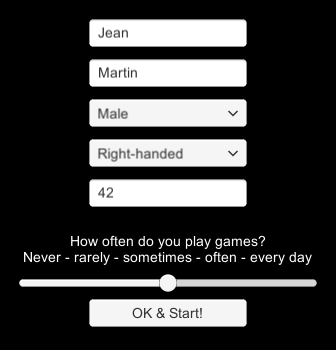
\includegraphics[width=0.4\textwidth]{figures/ch5/questionnaire}
%		\caption[Questionnaire]{Questionnaire soumis aux sujets de notre étude empirique, avant l'étude elle-même.}
%		\label{fig:questionnaire}
%	\end{figure}
	
	Les sujets devaient ensuite cliquer sur un bouton pour lancer l'expérience. La moitié (9) d'entre eux a complété la condition homogène d'abord, et hétérogène ensuite ; l'autre moitié (8) a complété ces conditions dans l'ordre inverse, afin de compenser d'éventuels effets d'apprentissage, par ailleurs palliés par la session d'entrainement préliminaire.
	
	Afin de tenter d'harmoniser les stratégies de sélection de nos sujets (c'est-à-dire de les rapprocher les unes des autres sur le continuum précision-vitesse), nous leur avons fourni pour consigne de tâcher de sélectionner chaque cible en moins de 10 essais. Cette valeur, délibérément élevée, fut choisie pour inciter les sujets à privilégier la vitesse, afin de réduire le temps de sélection par essai, et donc d'améliorer le ratio $\frac{nombre~d'essais}{temps~de~passation}$, attendu que la durée de l'expérience tend à augmenter la fatigue et la lassitude des sujets, surtout pour une tâche aussi répétitive et nécessitant un tel degré de concentration.
	
	Afin de limiter cette fatigue et cette lassitude, nous imposons une pause après la sélection de 25~\%{} des cibles, ainsi qu'après 50~\%{} et 75~\%{} d'entre elles. Chaque sujet est libre de laisser la pause durer aussi longtemps qu'il le souhaite, afin de récupérer pleinement. Une pression de la barre d'espace permet de reprendre les sélections de cibles. Une barre de progression affichant le taux de complétion de l'expérience est affichée en permanence au bas de l'écran, en vert, et lorsque tous les essais ont été effectués, un message s'affiche pour indiquer la fin de l'expérience et remercier les sujets.
	
	\subsection{Ajustement des tailles des cibles}
	Pour déterminer la taille optimale de chaque cible, nous nous sommes appuyés sur le modèle que nous proposions dans la section~\ref{sub:areaVperf}, en le simplifiant pour le rendre plus commode à utiliser. Nous utilisons toujours la même équation pour calculer l'espérance de l'aire de l'enveloppe convexe d'une cible, que nous reproduisons dans le chapitre présent, équation~\ref{eq:ch5areaModel}.
	
	\begin{equation}
		\mathbb{E}(\mathcal{A}(ec)) = V^{2}N \left( A\sqrt{F} \right)^n \left(1+\left(\frac{A\sqrt{F}}{x_n}\right)^{|\beta|s}\right)^{\frac{\operatorname{sgn}(\beta)}{s}}
		\label{eq:ch5areaModel}
	\end{equation}
	
	Nos précédents travaux nous permettent de supposer qu'une parabole \og inversée \fg{} (i.e. croissante, puis décroissante) fonction de $\mathbb{E}(\mathcal{A}(ec))$ fournit une approximation utile du temps de sélection d'une cible (voir la figure~\ref{fig:perf_V_RealArea_better_fit}, section~\ref{sub:areaVperf}). Il est donc possible, sur le principe, d'utiliser la valeur de cette parabole comme facteur d'agrandissement/rétrécissement d'une cible. En l'état, toutefois, cette parabole présente quelques inconvénients.
	
	Premièrement, ses valeurs, entièrement comprises dans l'intervalle [0,05 ; 0,35] ne fournissent pas des facteurs directement utilisables. Deuxièmement, l'application de tels facteurs mènerait à un rétrécissement de toutes les cibles qui, même s'il était compensé par un agrandissement uniforme après (i.e. appliquant le même facteur à toutes les cibles) ne garantirait pas la constance de la somme des aires de toutes les cibles. Troisièmement, l'intervalle d'antécédents pour lesquels la parabole est utile, et son point de symmétrie ne sont pas clairs. Enfin, il n'est pas évident que le facteur d'agrandissement d'une cible doive être proportionnel à l'estimation du temps de sélection --- peut-être une parabole plus \og plate \fg{} fournirait-elle de meilleurs résultats, ou, au contraire, peut-être une parabole plus \og aiguë \fg{} serait-elle plus appropriée.
	
	Nous avançons donc qu'une bonne fonction d'ajustement des tailles devrait :
	
	\begin{itemize}
		\item Être parabolique, croissante, puis décroissante,
		\item Être utile sur l'intervalle [0 ; 1], avec un maximum en 0,5 qui soit également son point de symmétrie,
		\item Être ajusteable à l'aide d'un paramètre simple, afin d'être plus ou moins plate ou aiguë,
		\item Ne pas modifier la somme des aires de toutes les cibles --- ce qui est équivalent au fait que l'intégrale de la fonction vaille 1 sur l'intervalle [0 ; 1].
	\end{itemize}
	
	\subsubsection{Parabole inversée d'intégrale unitaire}
	Nous proposons donc la fonction de l'équation~\ref{eq:scalingParabola}, qui remplit tous les critères :
	
	\begin{equation}
		p(N,x) = \frac{1}{1-\frac{N}{12}} \left(1-N\left(x-\frac{1}{2}\right)^2\right)
		\label{eq:scalingParabola}
	\end{equation}
	
	La figure~\ref{fig:parabolae} illustre le comportement de cette fonction sur l'intervalle [0 ; 1] en fonction de la valeur de N, librement choisie entre 0 et 4. Celle-ci permet d'ajuster l'allure de la parabole, et donc la mesure dans laquelle ce procédé agrandit les cibles \og difficiles \fg{} et rétrécit les cibles \og faciles \fg{}. Pour un effet prononcé, on optera donc pour une valeur proche de 4, tandis que l'on préférera une valeur proche de 0 pour un effet plus léger.
	
	Attention toutefois, la constance de la somme des aires de toutes les cibles n'est garantie que si celles-ci sont réparties uniformément sur l'intervalle normalisé de leurs aires.\footnotemark{} En pratique, ce n'est généralement pas le cas, et une légère correction doit s'appliquer. Pour cela, nous mesurons cette somme des aires avant l'ajustement des tailles, puis après, et appliquons un petit correctif uniforme à la hausse ou à la baisse, selon le cas rencontré. Ce correctif permet aussi d'appliquer le facteur d'ajustement de taille non pas à l'aire d'une cible mais, dans un souci de simplicité, au rayon de chaque cible. À l'issue de plusieurs pilotes, nous avons choisi la valeur $N=2$. Ce choix informé par des essais empiriques n'est pas nécessairement optimal.

	
	\footnotetext{La normalisation doit se faire par rapport au maximum d'espérance de l'aire d'une enveloppe convexe de trajectoire, correspondant à $A\sqrt{F} = 120$.}
	
	\begin{figure}[!htb]
		%\centering
		\begin{subfigure}[t]{0.49\textwidth}
			\centering
			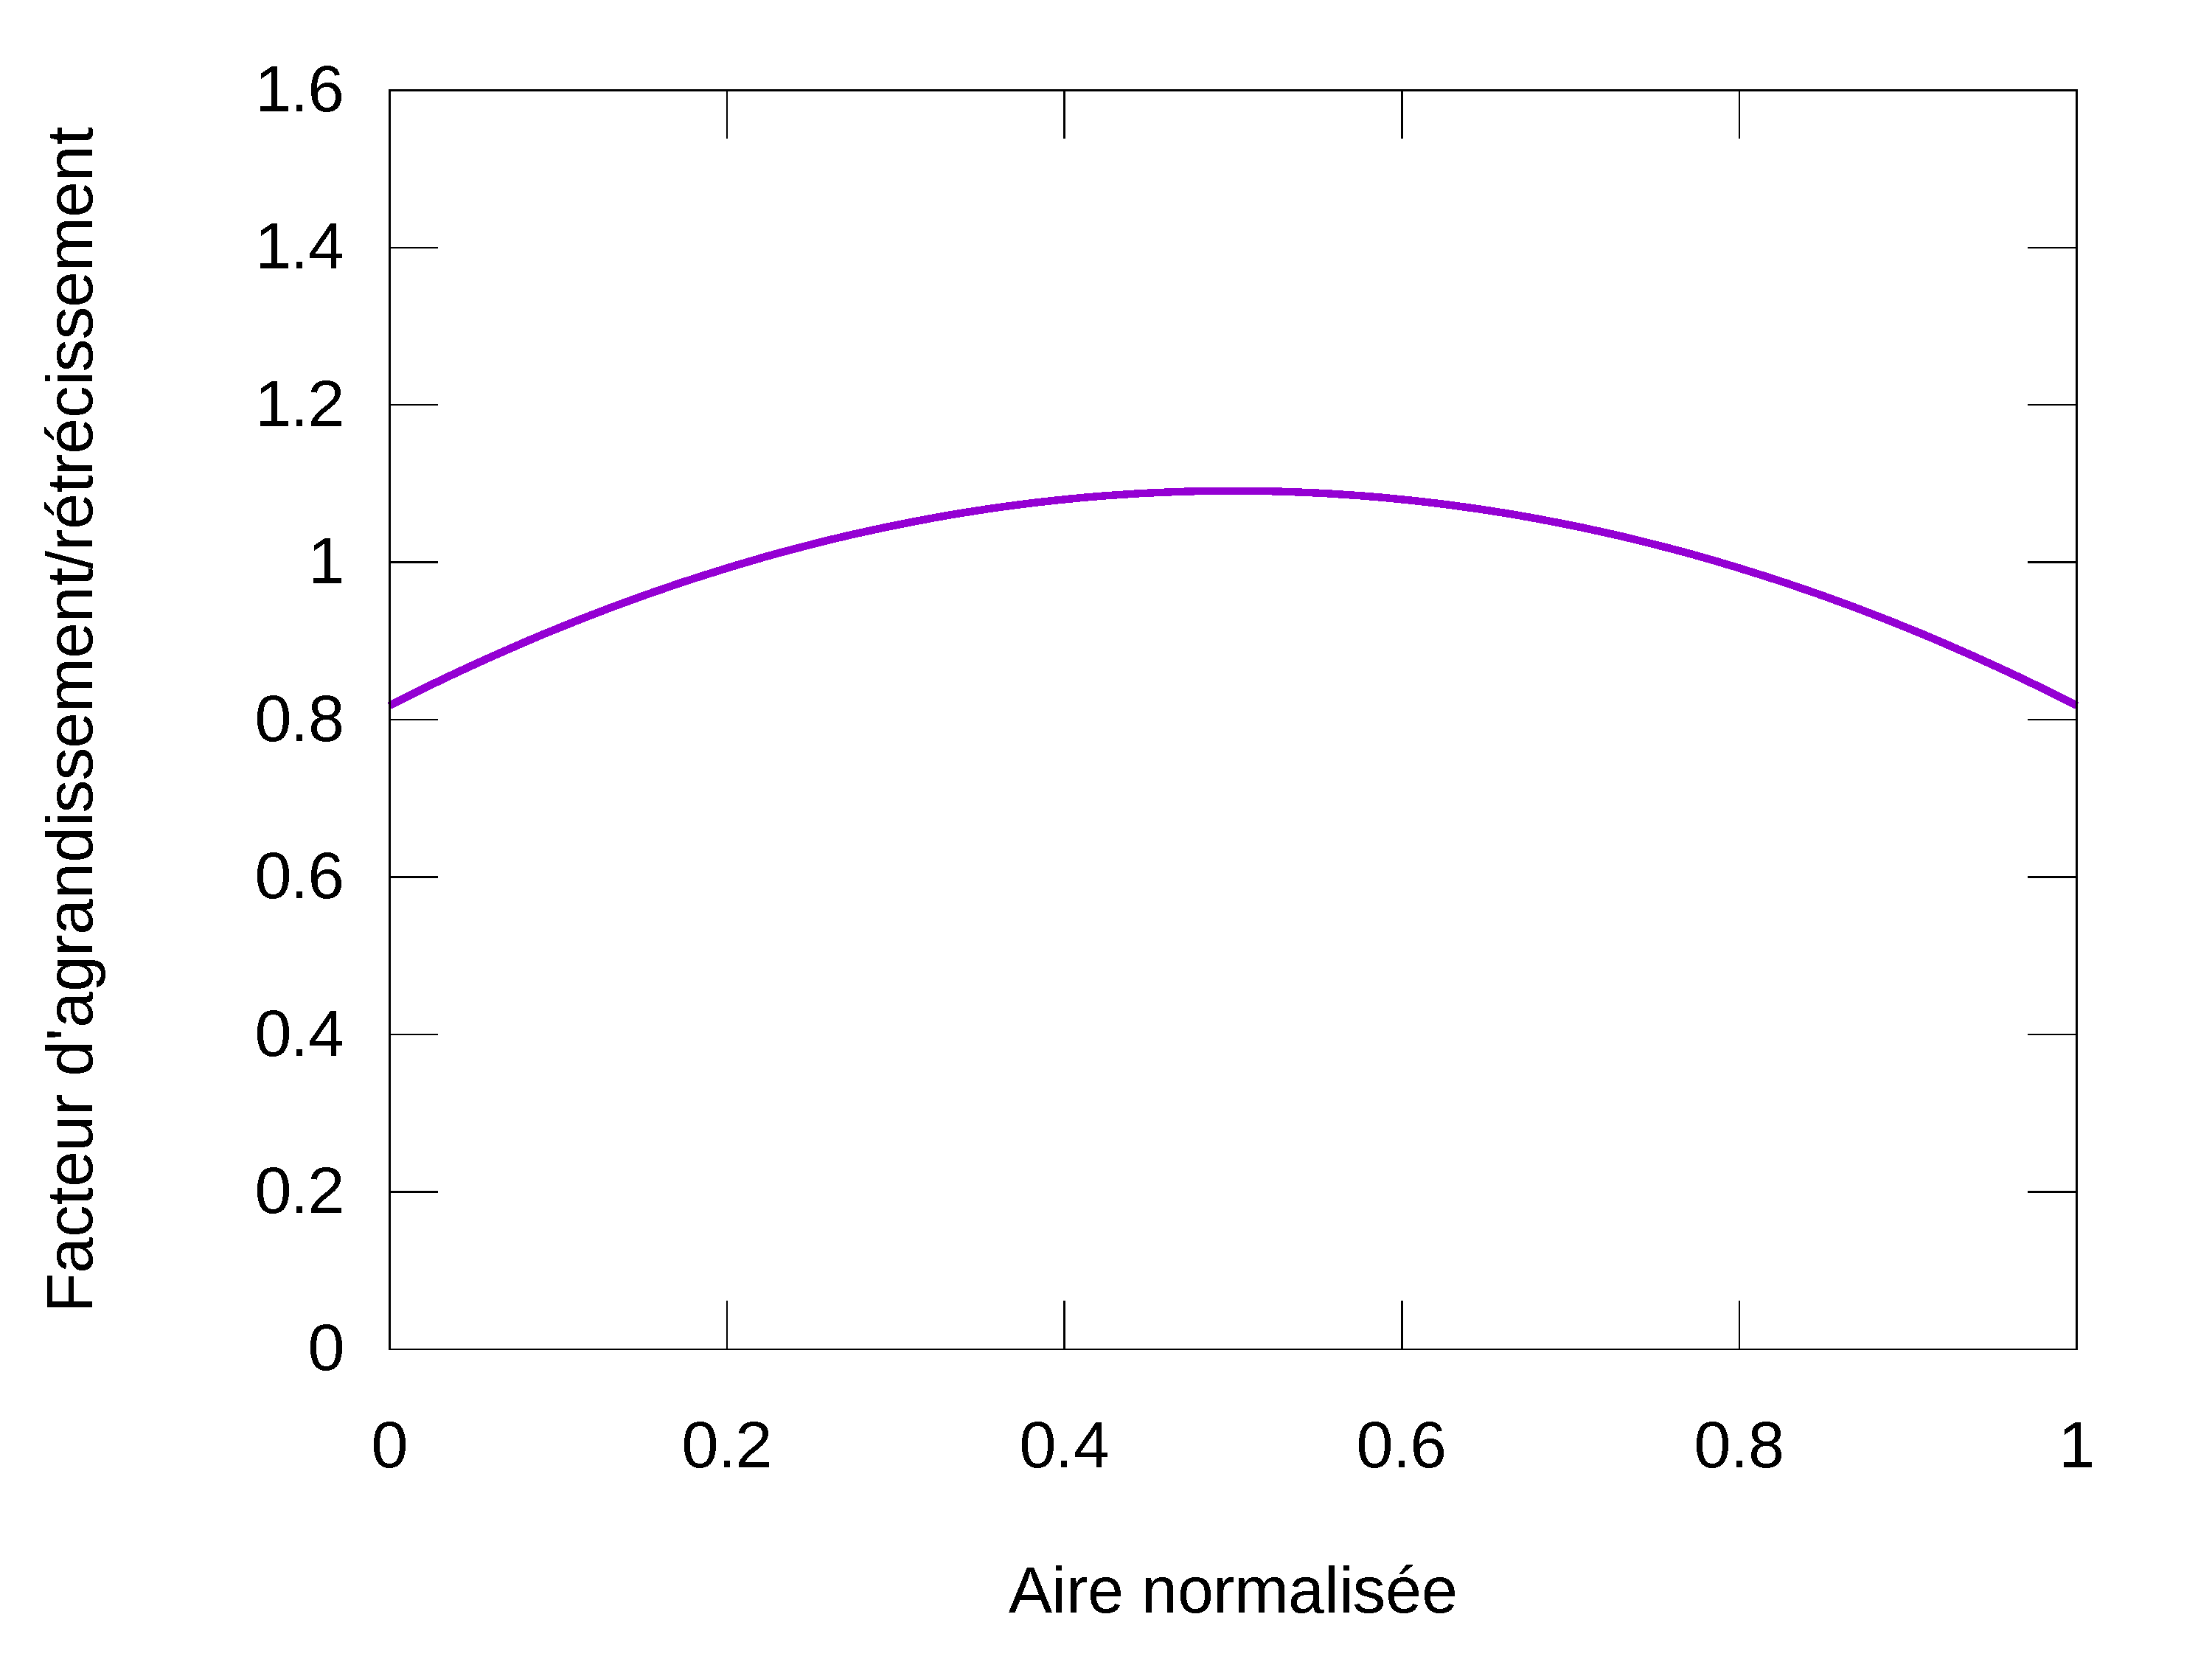
\includegraphics[width=\textwidth]{figures/ch5/parabola1}
			\caption{$N=1$.}
			\label{fig:parabola1}
		\end{subfigure}
		~
		\begin{subfigure}[t]{0.49\textwidth}
			\centering
			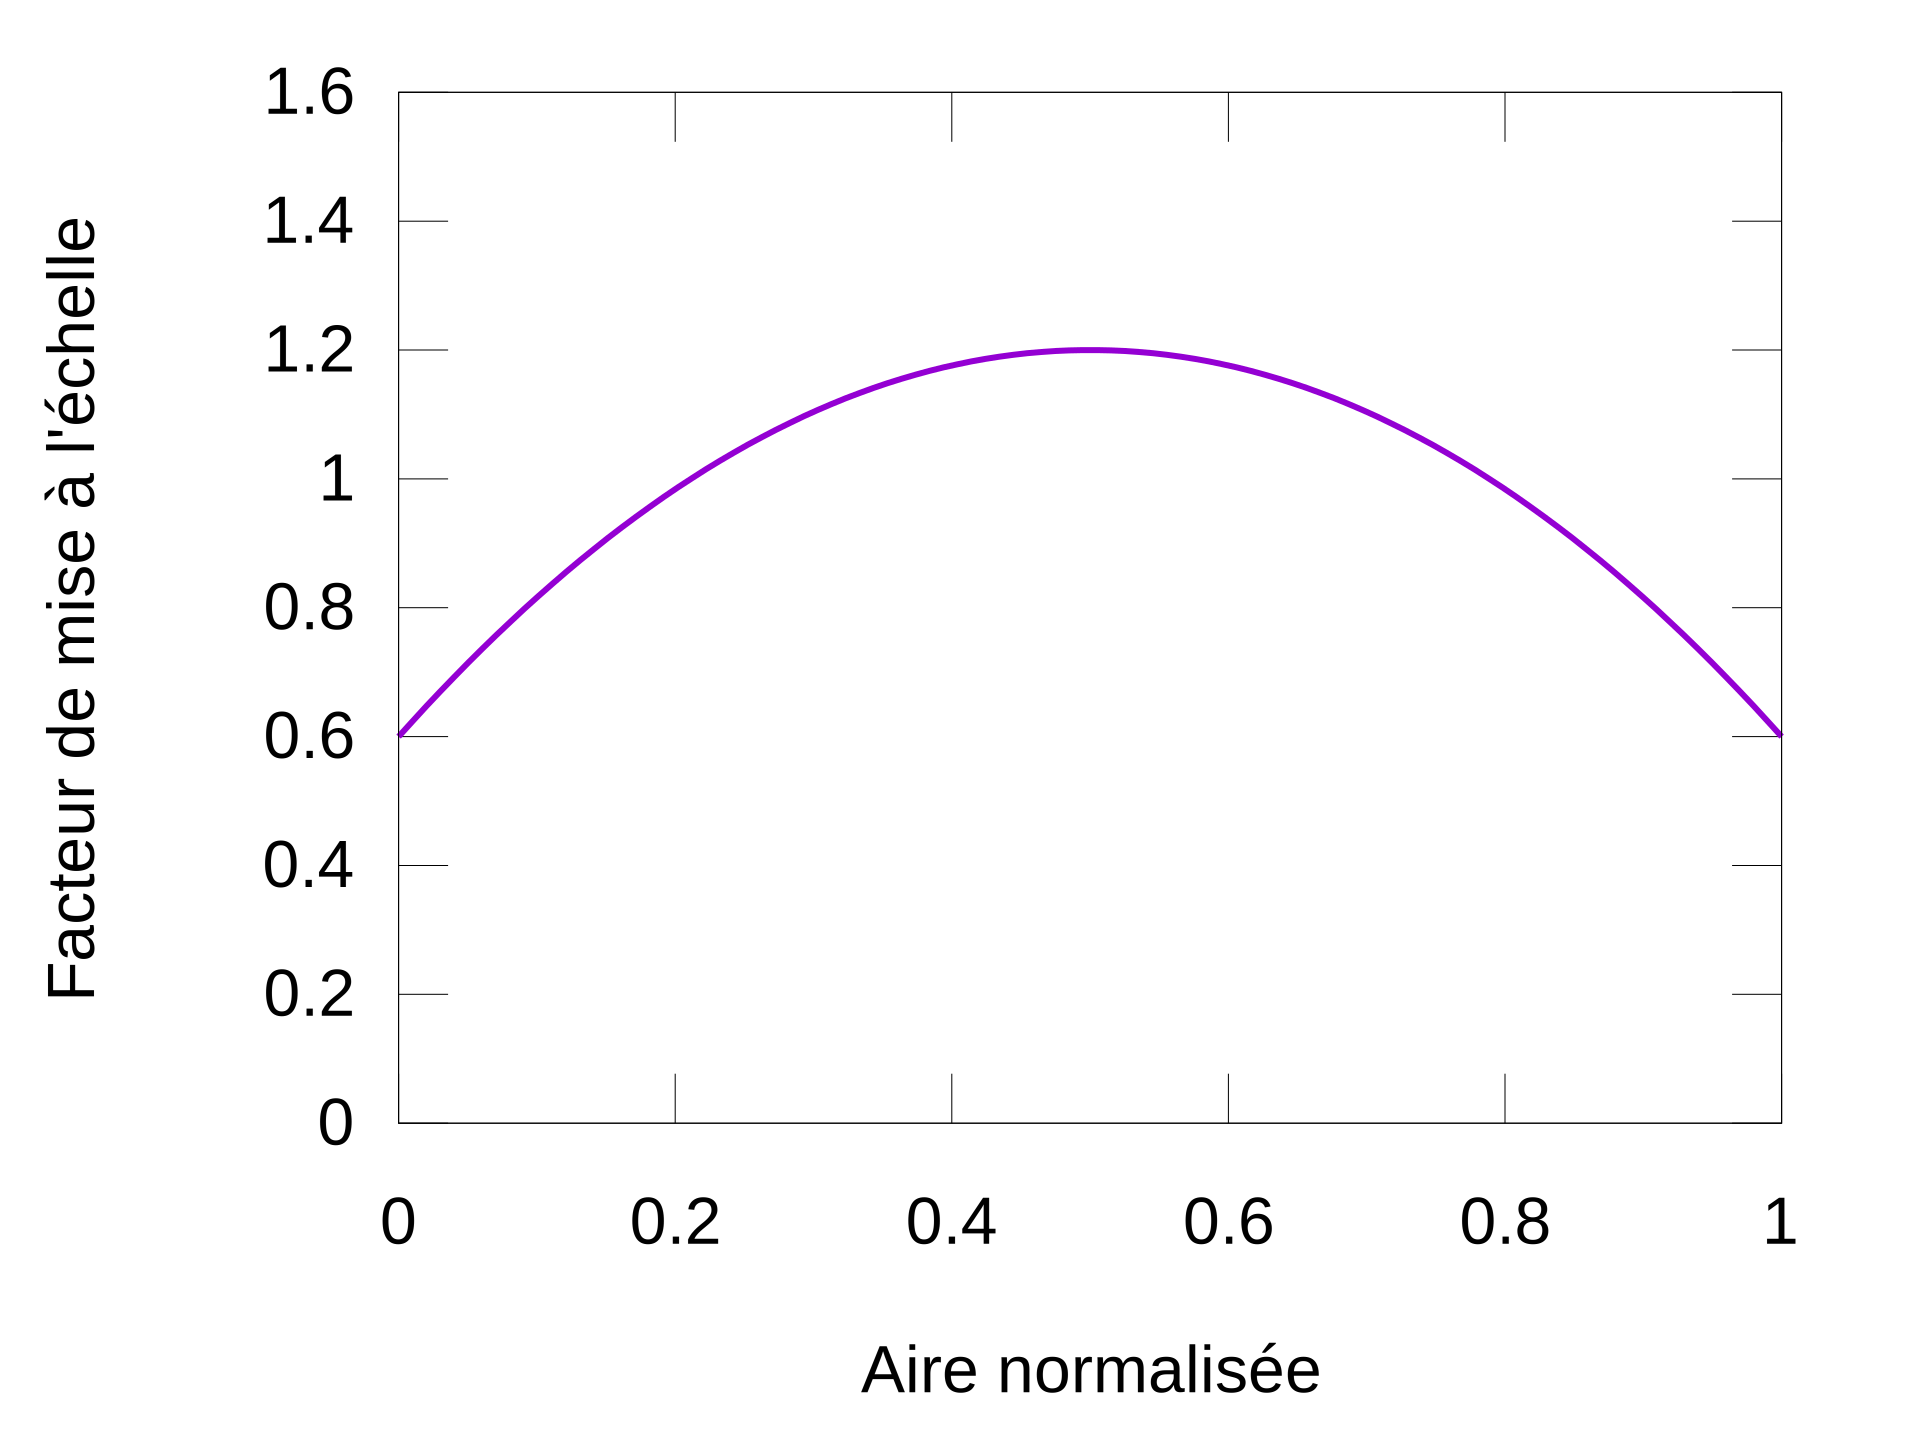
\includegraphics[width=\textwidth]{figures/ch5/parabola2}
			\caption{$N=2$.}
			\label{fig:parabola2}
		\end{subfigure}
		~
		\begin{subfigure}[t]{0.49\textwidth}
			\centering
			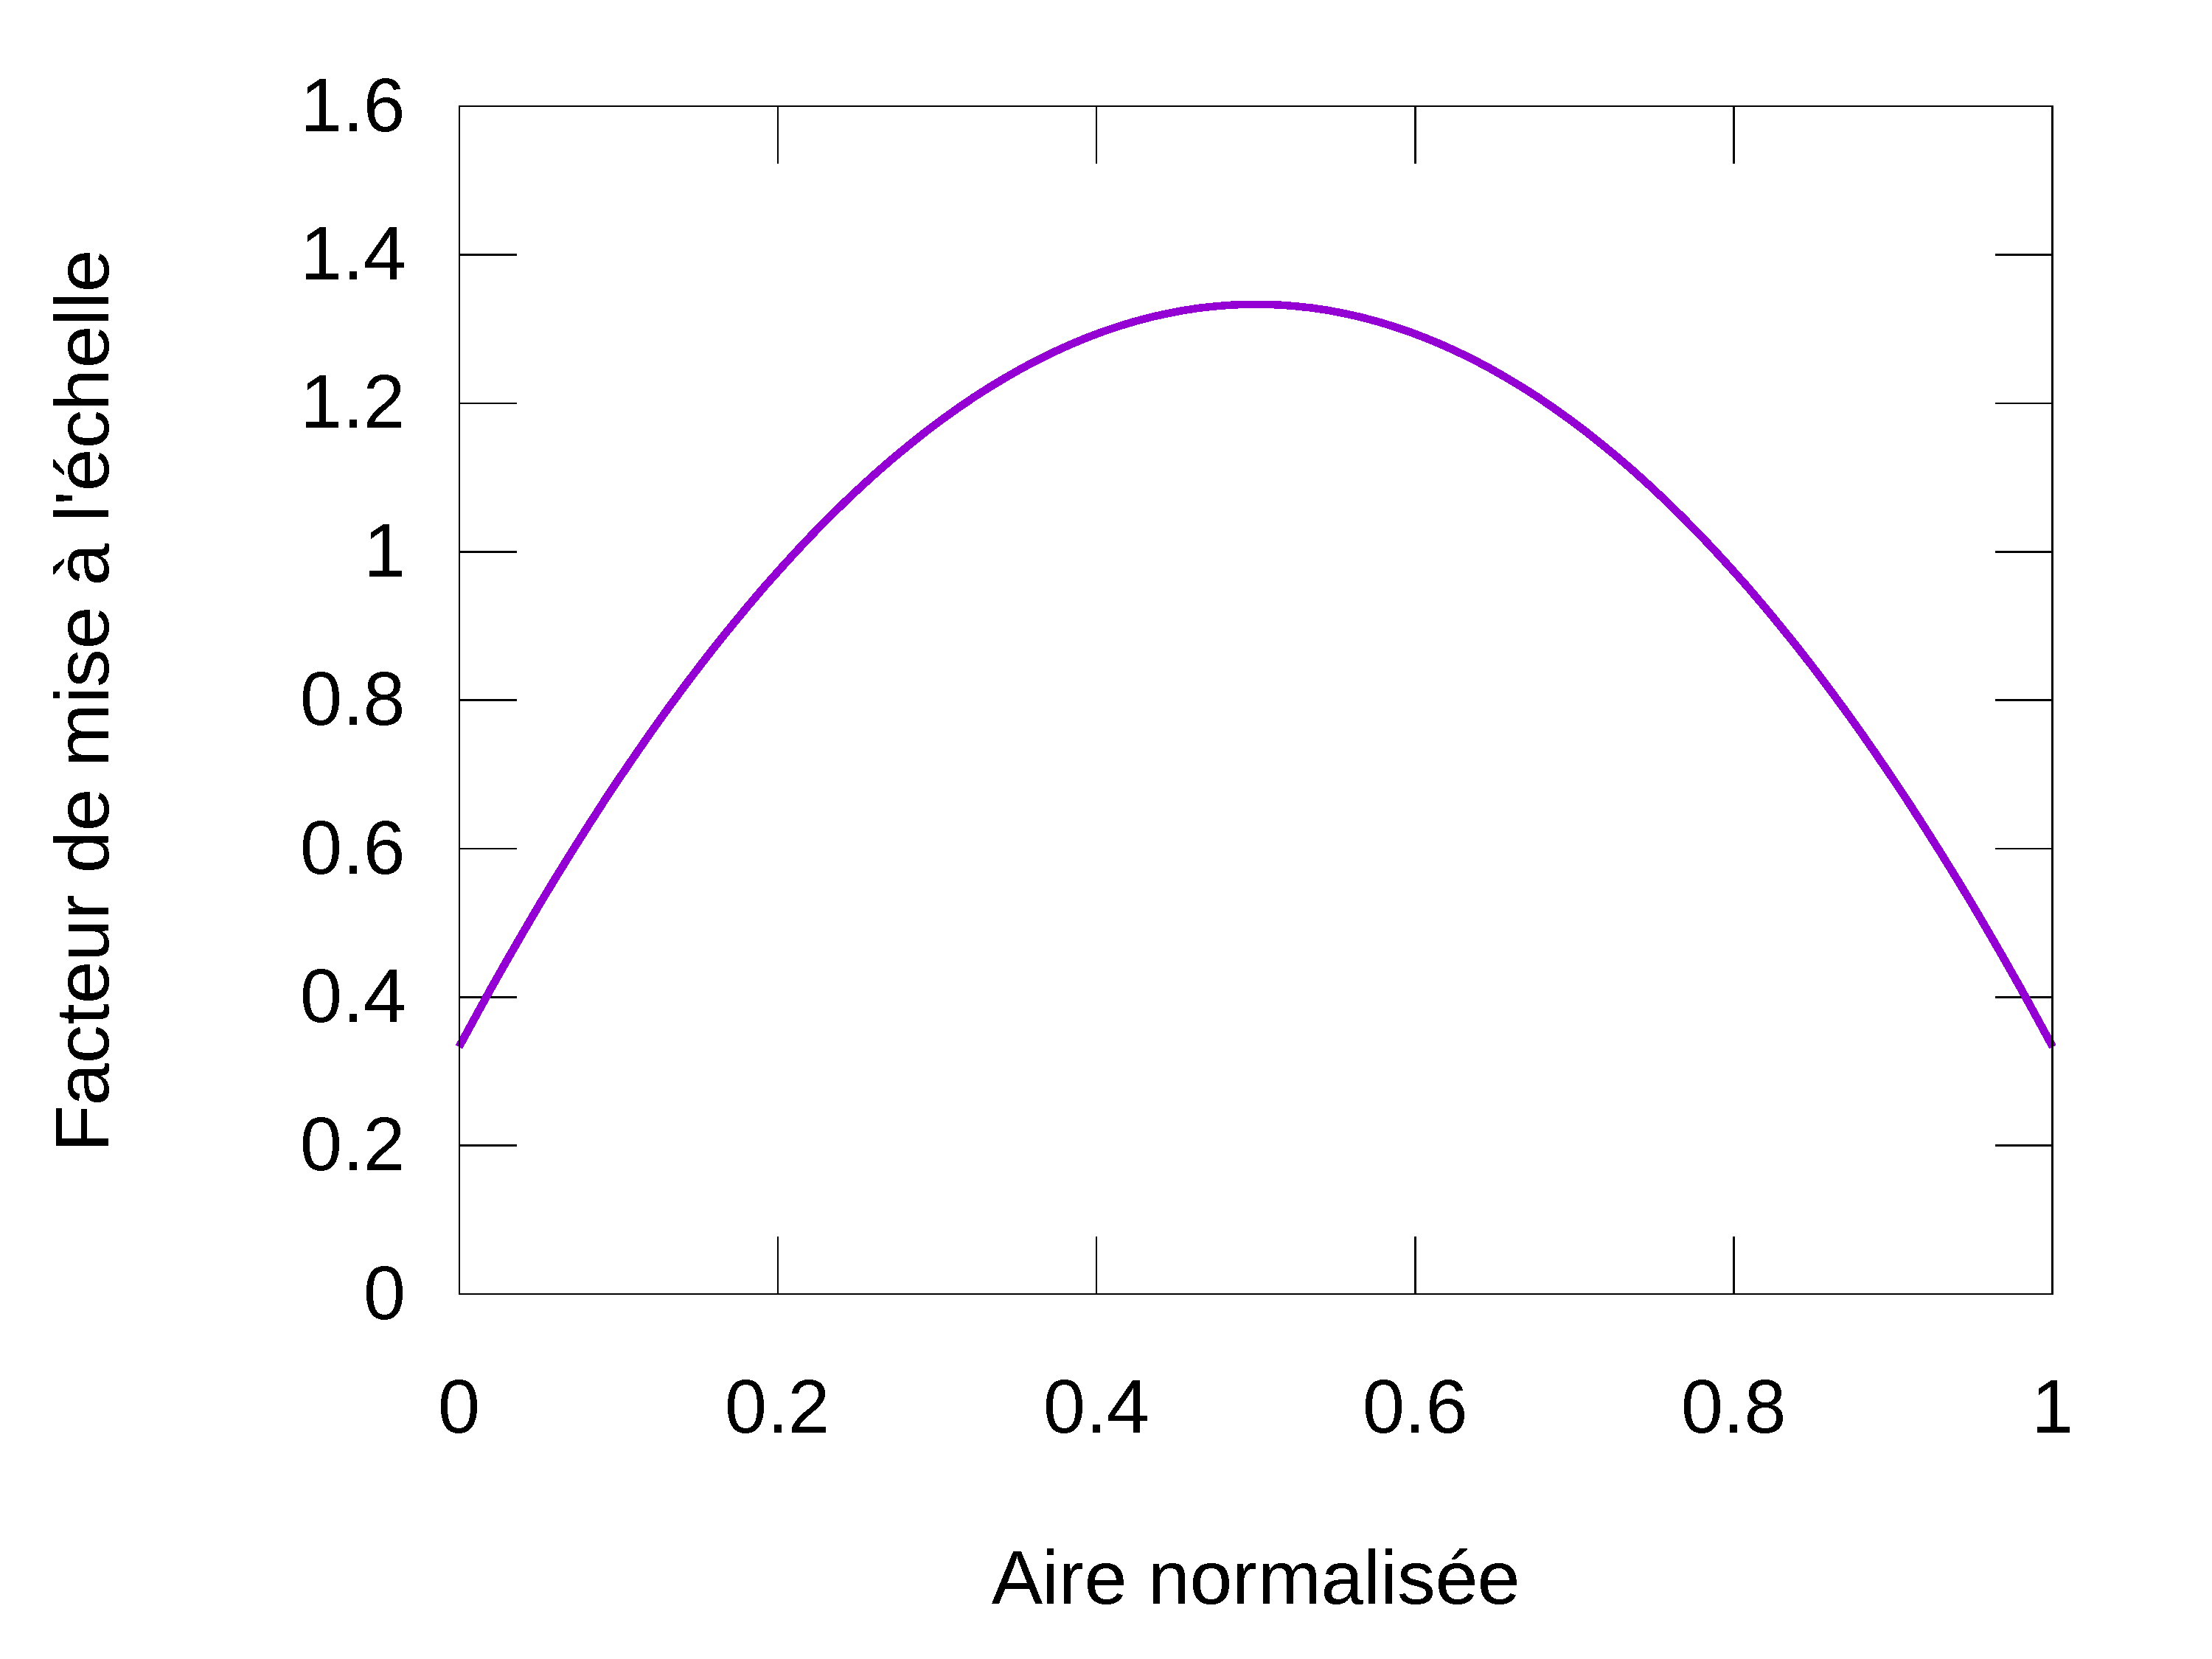
\includegraphics[width=\textwidth]{figures/ch5/parabola3}
			\caption{$N=3$.}
			\label{fig:parabola3}
		\end{subfigure}		
		~
		\begin{subfigure}[t]{0.49\textwidth}
			\centering
			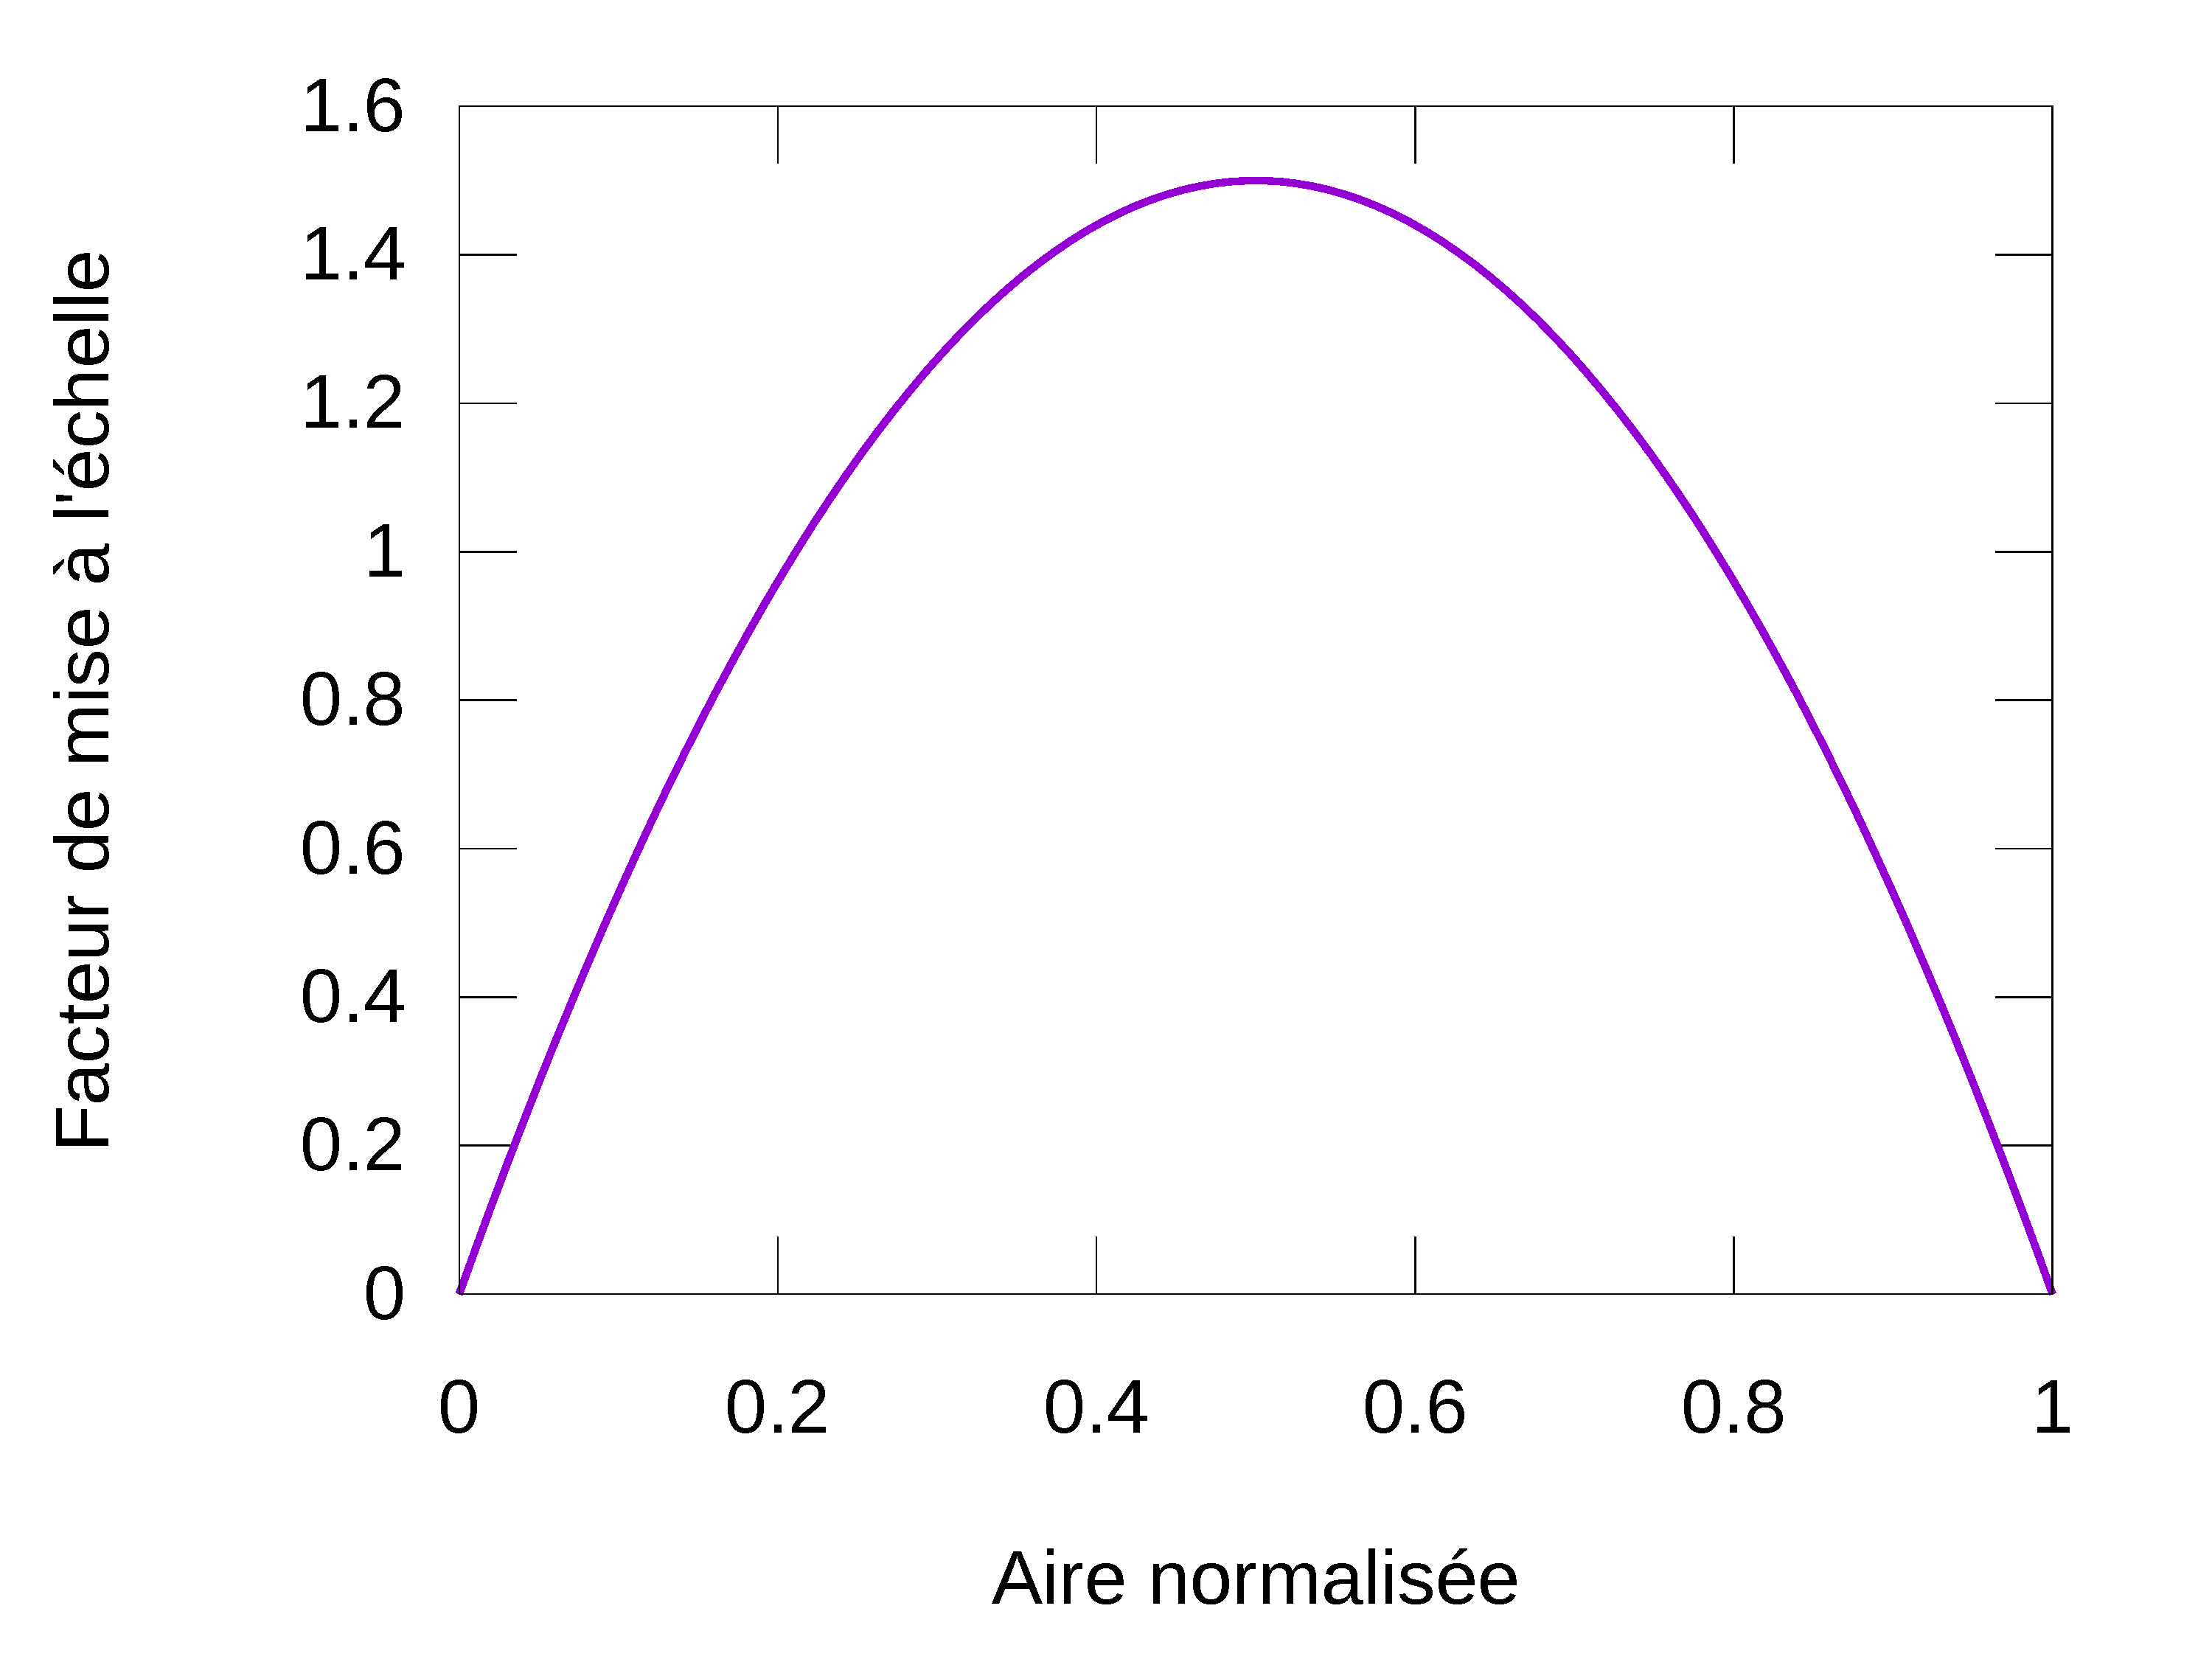
\includegraphics[width=\textwidth]{figures/ch5/parabola4}
			\caption{$N=4$.}
			\label{fig:parabola4}
		\end{subfigure}
		\caption[Paraboles pour ajuster les tailles des cibles]{Paraboles pour ajuster les tailles des cibles.}
		\label{fig:parabolae}
	\end{figure}
		
	\subsubsection{Données collectées}
	Nous avons collecté de nombreuses données, certaines sont constantes, d'autres sont liées à des événements ou synthétiques, et certaines changent à chaque tour de boucle du logiciel d'évaluation, c'est-à-dire 60 fois par seconde.
	
	Les données constantes sont les suivantes :
	
	\begin{itemize}
		\item Les paramètres VFA de chaque cible ;
		\item L'espérance de l'aire de l'enveloppe convexe de chaque cible, d'après ses paramètres VFA ;
		\item L'estimation de la difficulté de sélection de chaque cible, d'après notre modèle.
	\end{itemize}
	
	Les données liées à des événements ou synthétiques sont les suivantes :
	
	\begin{itemize}
		\item Le temps de sélection de chaque cible, pour chaque essai ;
		\item Le nombre d'erreur pour chaque cible, pour chaque essai.
	\end{itemize}
	
	Les données collectées à chaque tour de boucle sont les suivantes :
	
	\begin{itemize}
		\item Le temps écoulé depuis le début de l'expérience (pauses exclues) ;
		\item La position de chaque cible dans les coordonnées du monde ;
		\item La position de chaque cible dans les coordonnées de l'écran ;
		\item La direction de chaque cible dans les coordonnées de l'écran ;
		\item La position du curseur dans les coordonnées du monde ;
		\item La position du curseur dans les coordonnées de l'écran ;
		\item La cible que l'utilisateur est actuellement censé sélectionner (celle qui est rouge) ;
		\item Une valeur booléenne indiquant si l'utilisateur a cliqué sur sa souris pendant la dernière \emph{frame} ;
		\item Une valeur booléenne indiquant si l'utilisateur a cliqué sur la cible rouge pendant la dernière \emph{frame} ;
		\item Le nombre d'erreurs pendant la dernière \emph{frame}.
	\end{itemize}
	
	\subsection{Résultats}
	\label{sub:as_res}
	Les données collectées les plus importantes sont les temps de sélection, et les erreurs. Nous allons dans un premier temps les examiner séparément, puis ensemble.
	
	\begin{figure}[!htb]
		%\centering
		\begin{subfigure}[t]{0.49\textwidth}
			\centering
			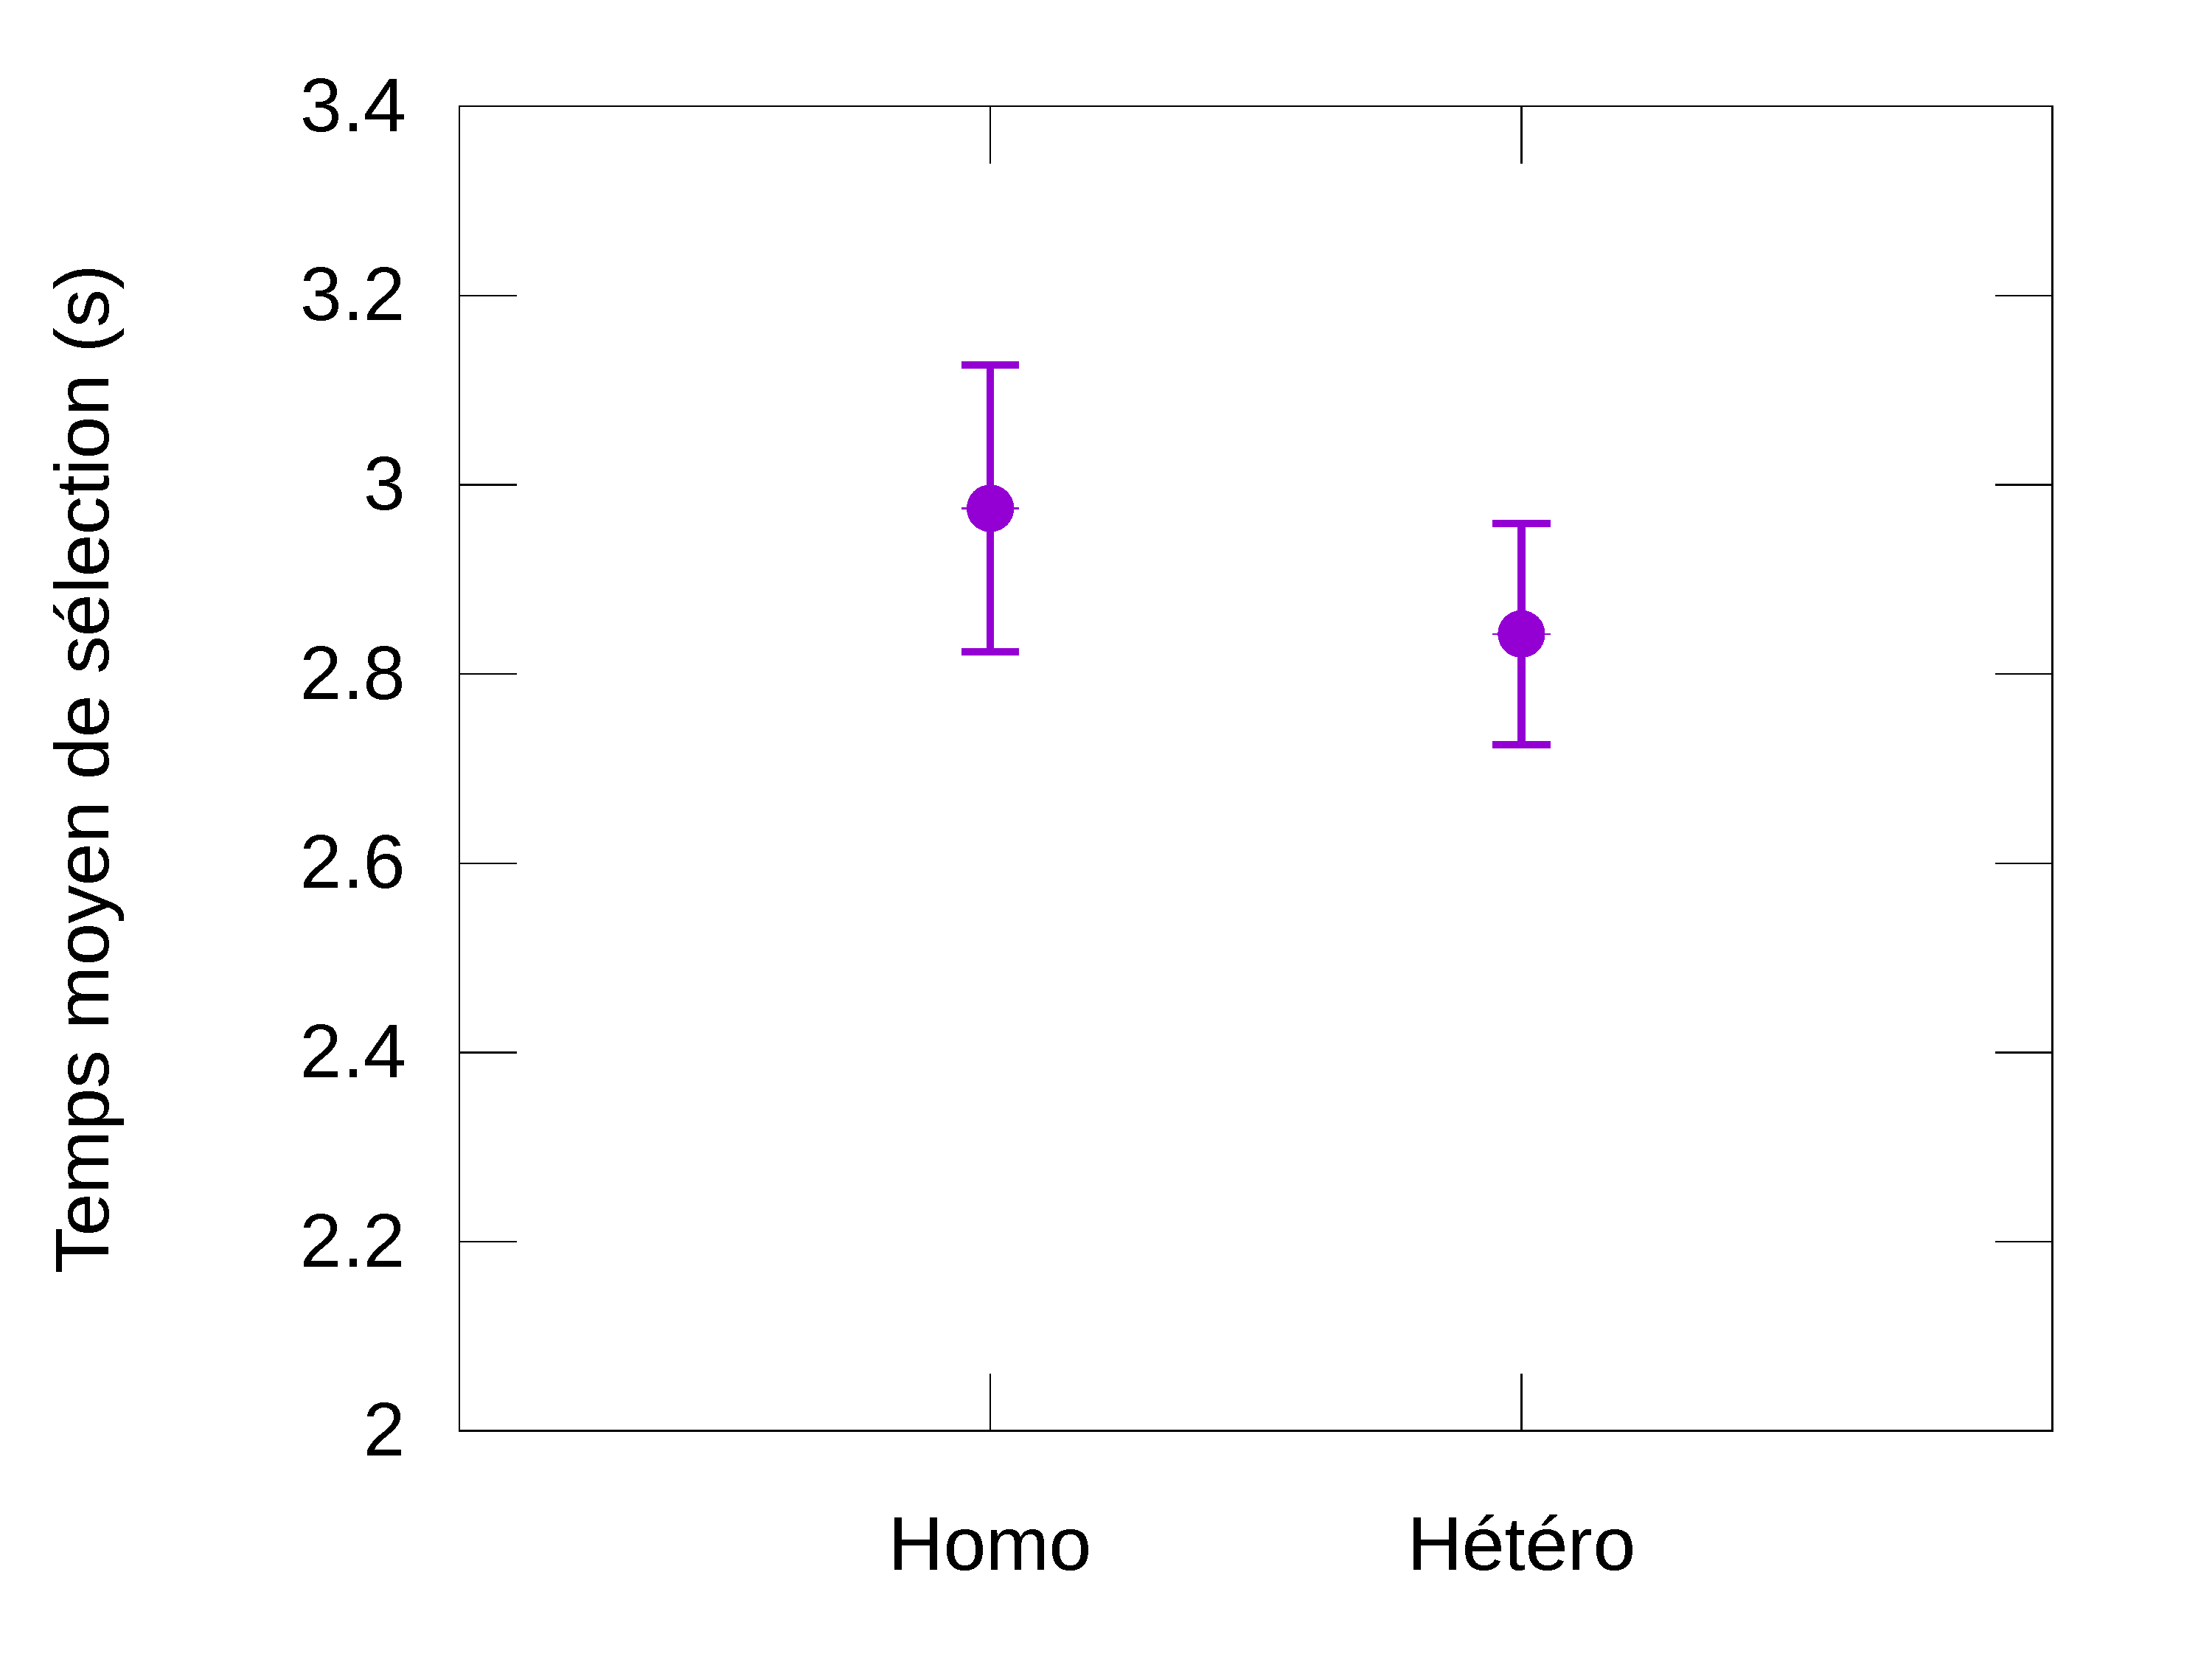
\includegraphics[width=\textwidth]{figures/ch5/timeRes}
			\caption{Temps moyens de sélection, et IC à 95~\%{}.}
			\label{fig:timeRes}
		\end{subfigure}
		~
		\begin{subfigure}[t]{0.49\textwidth}
			\centering
			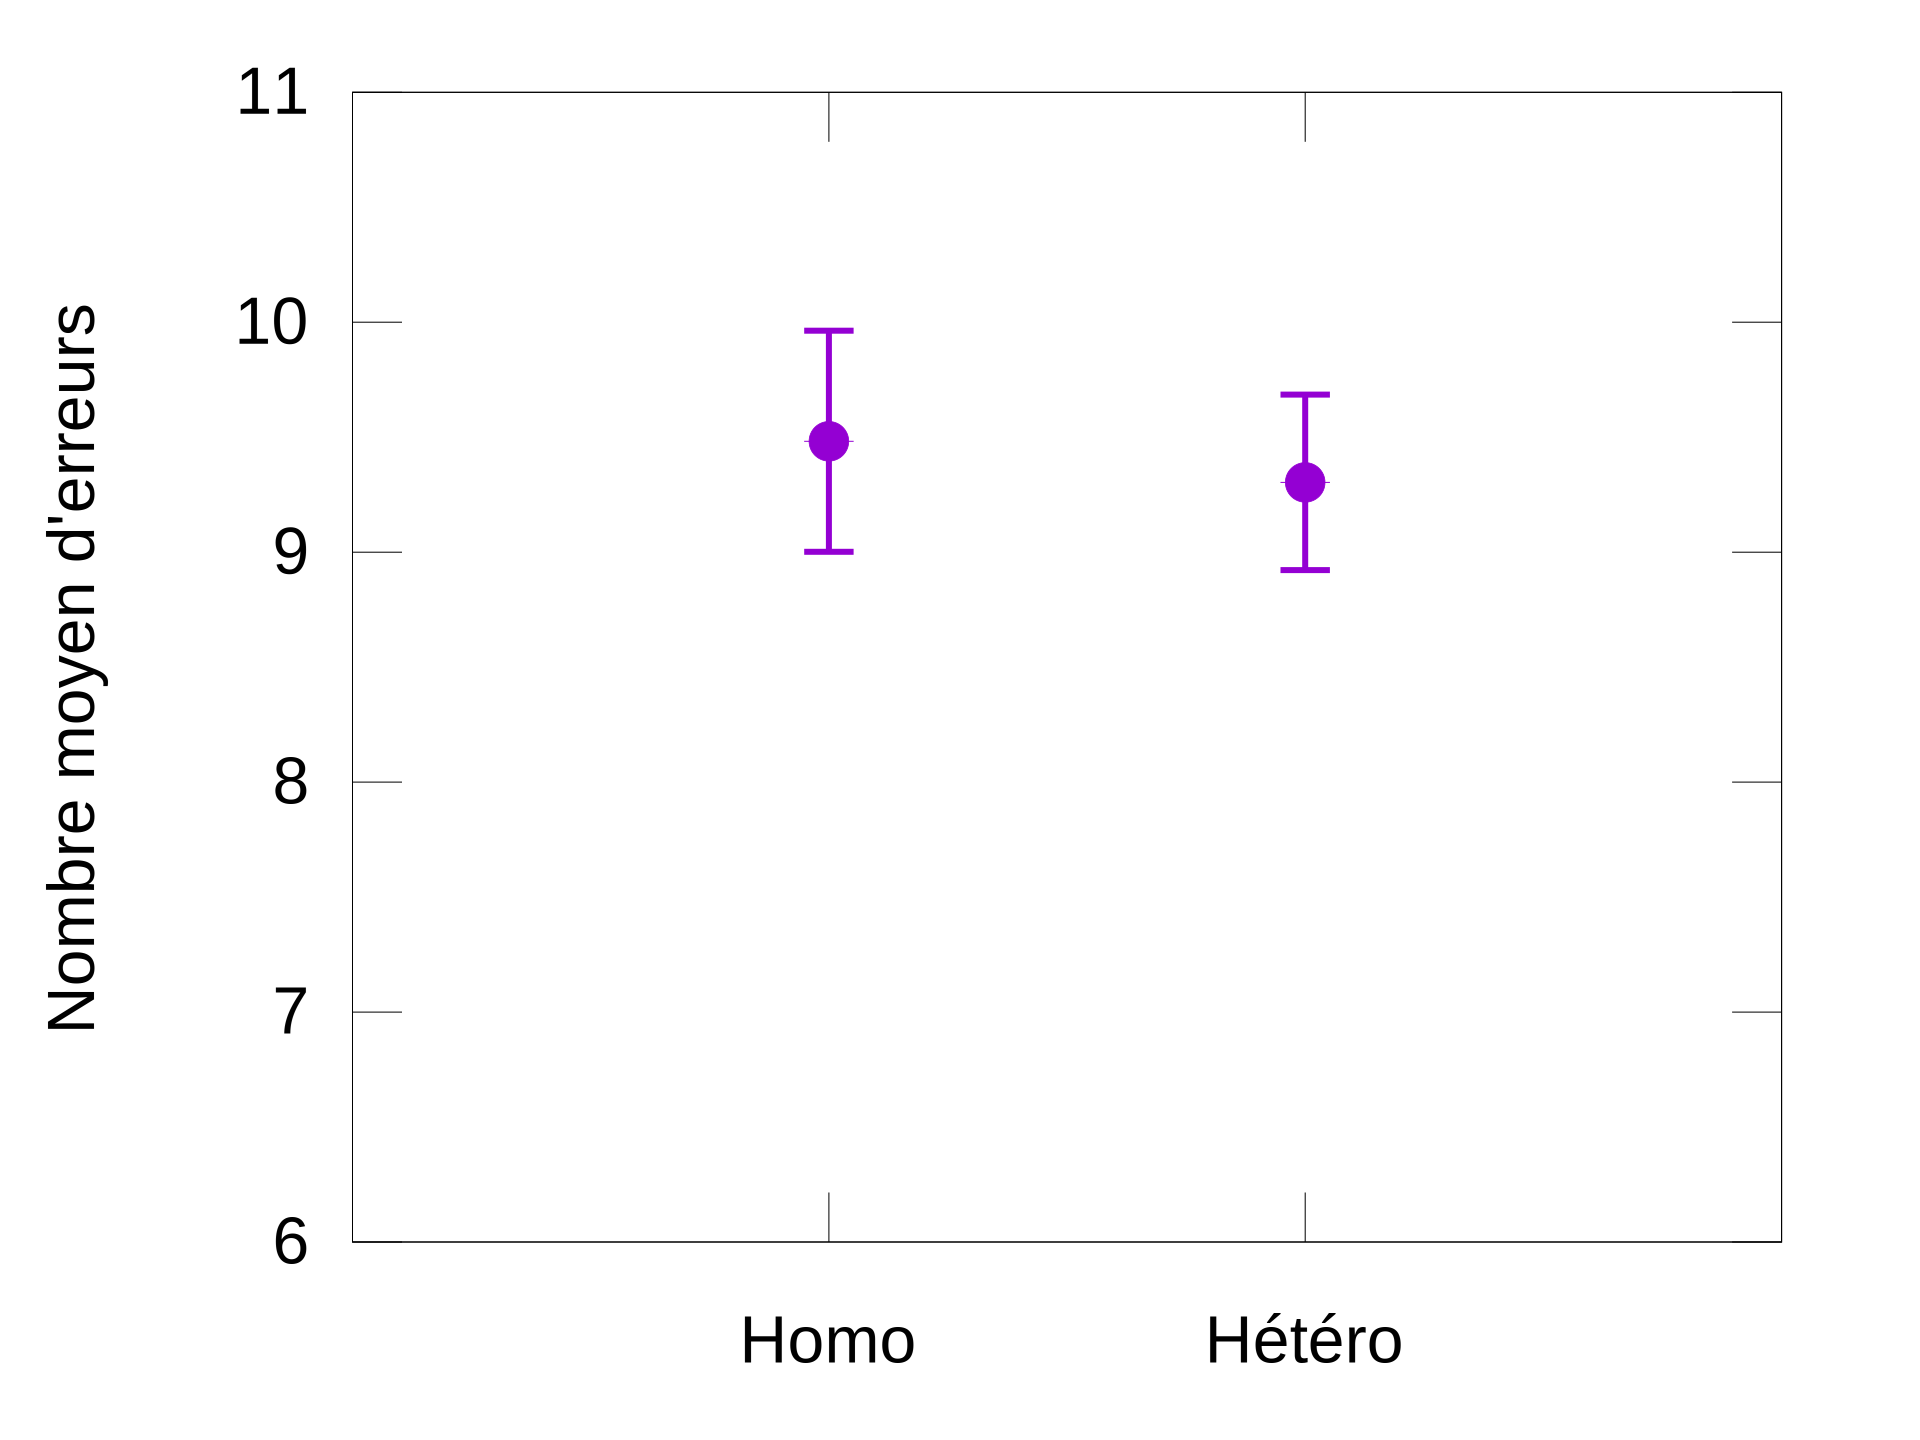
\includegraphics[width=\textwidth]{figures/ch5/errorRes}
			\caption{Nombres moyens d'erreurs, et IC à 95~\%{}.}
			\label{fig:errorRes}
		\end{subfigure}
		~
		\begin{subfigure}[t]{0.49\textwidth}
			\centering
			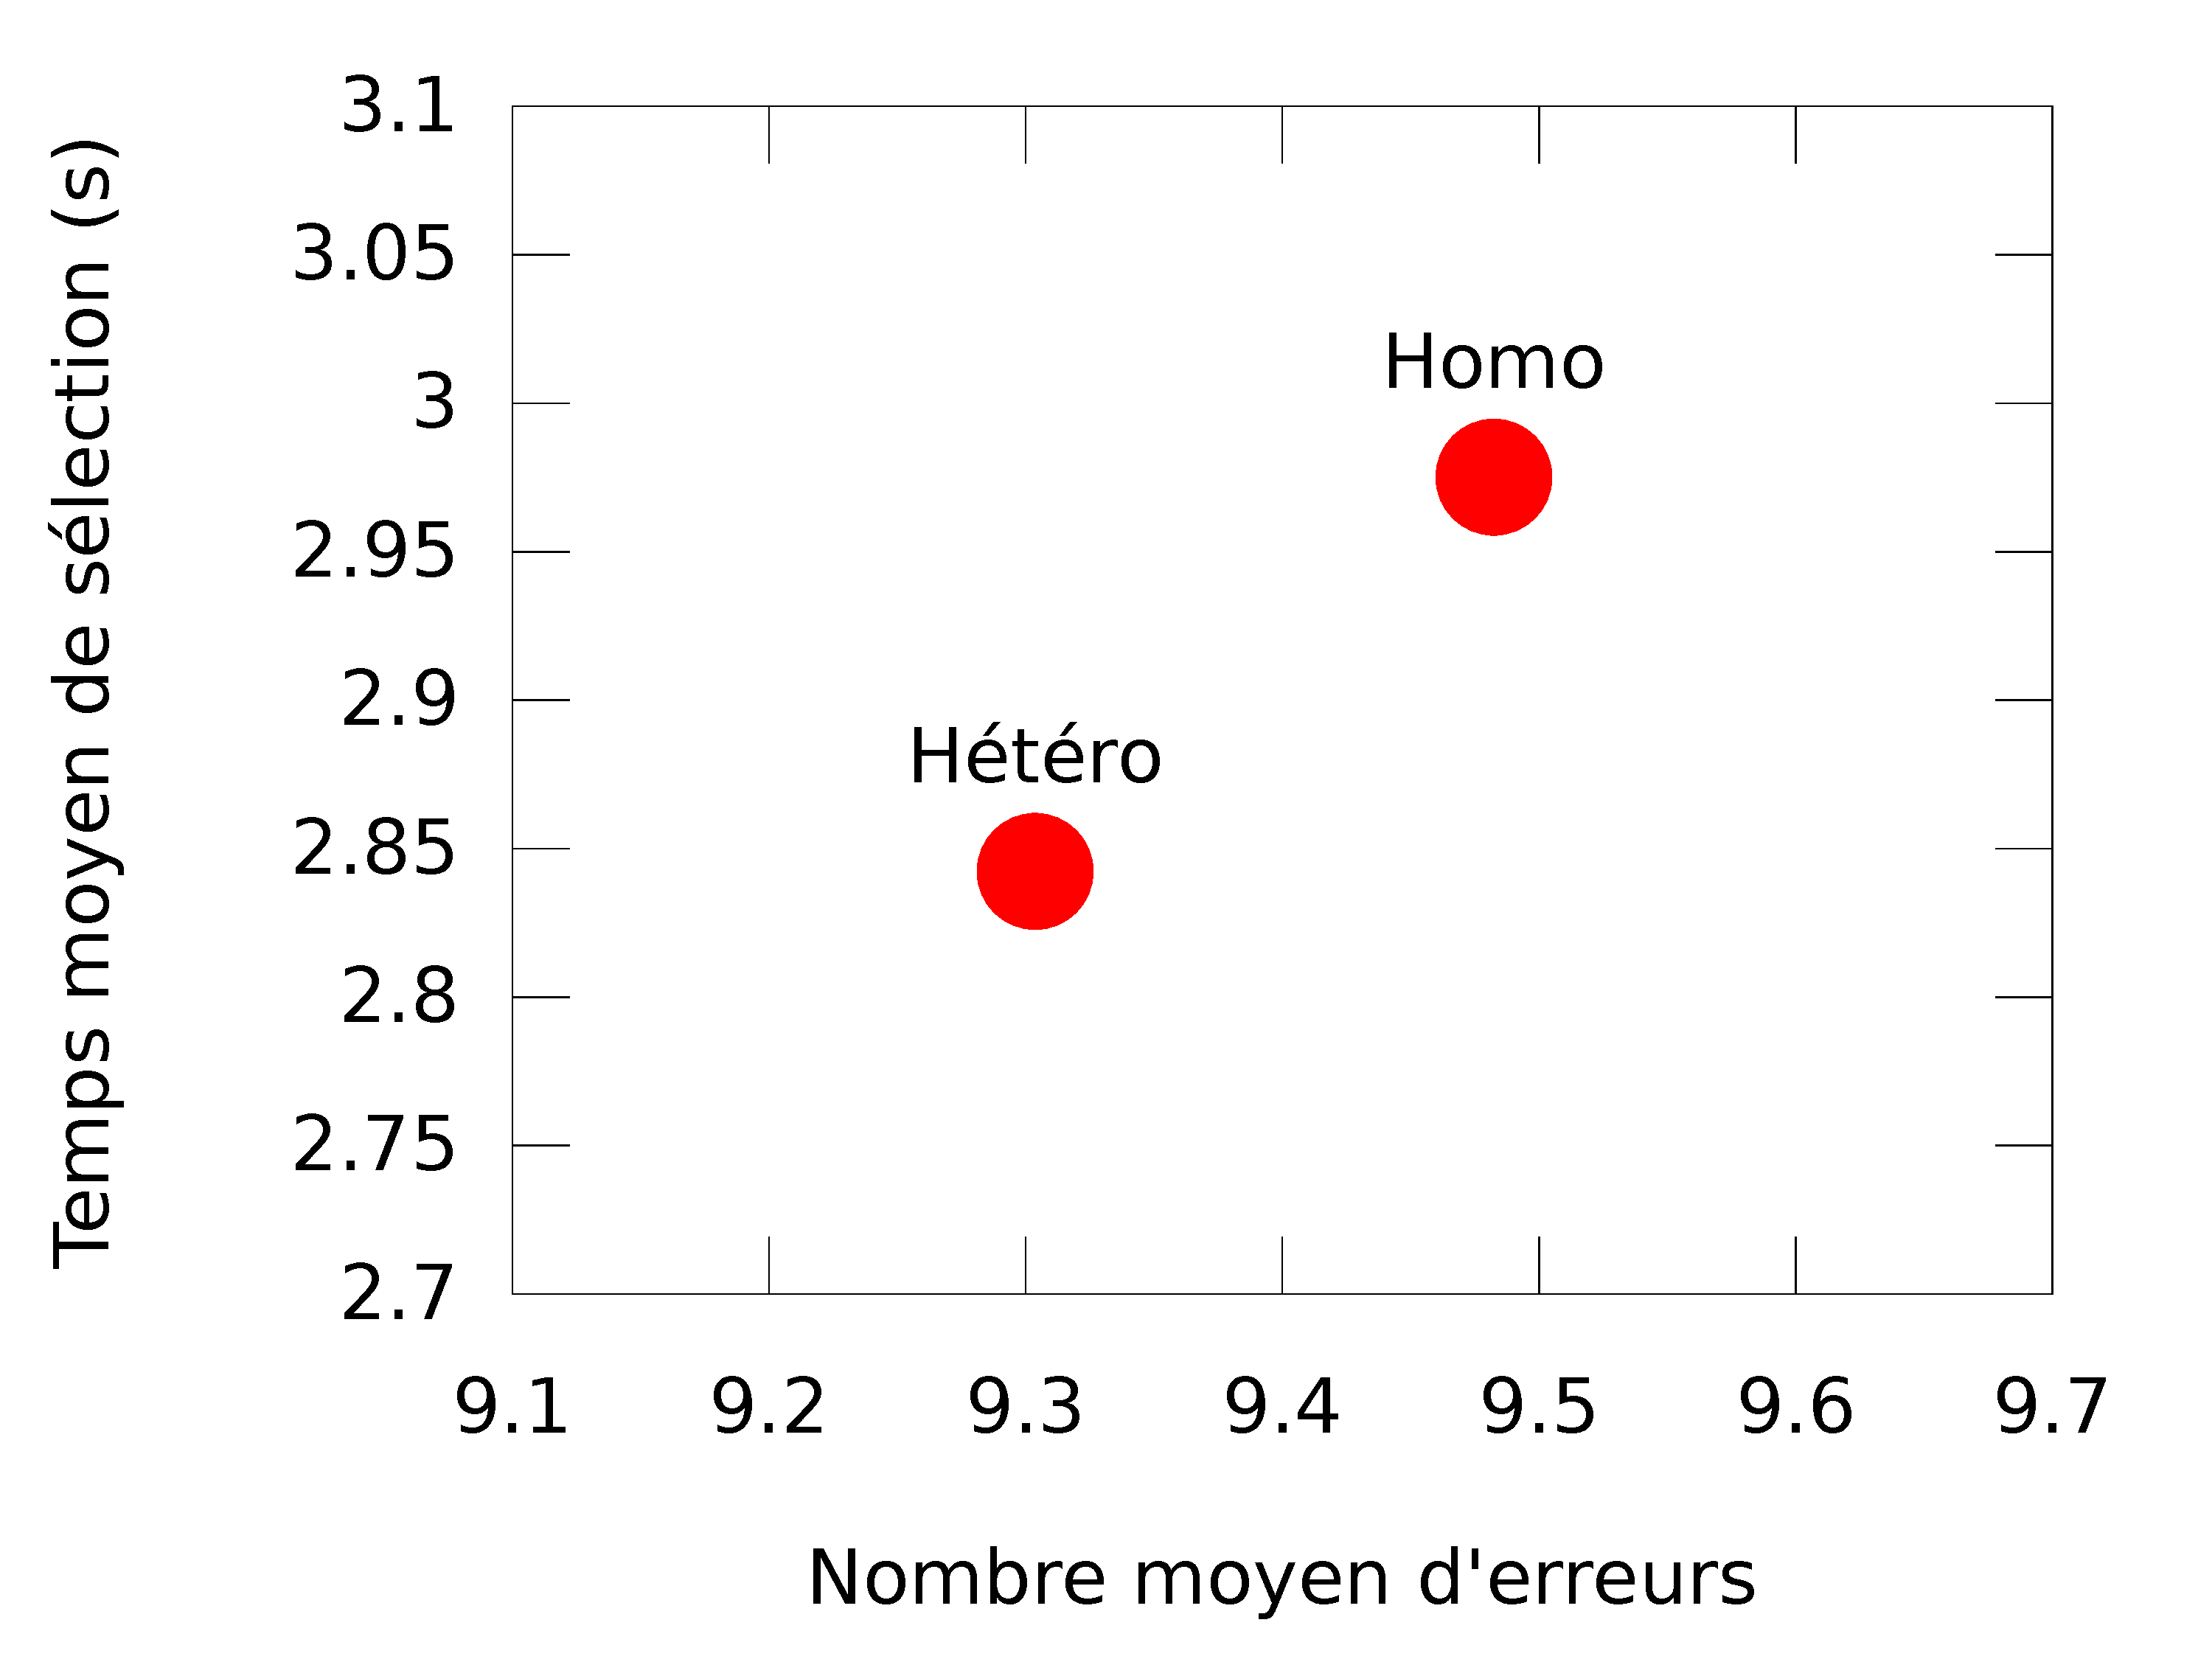
\includegraphics[width=\textwidth]{figures/ch5/errorsTimesScatter}
			\caption{Temps moyens de sélection et nombres moyens d'erreurs. Une technique \og idéale \fg{} serait située dans le coin inférieur gauche : temps courts, et peu d'erreurs.}
			\label{fig:errorsTimesScatter}
		\end{subfigure}
		~
		\begin{subfigure}[t]{0.49\textwidth}
			\centering
			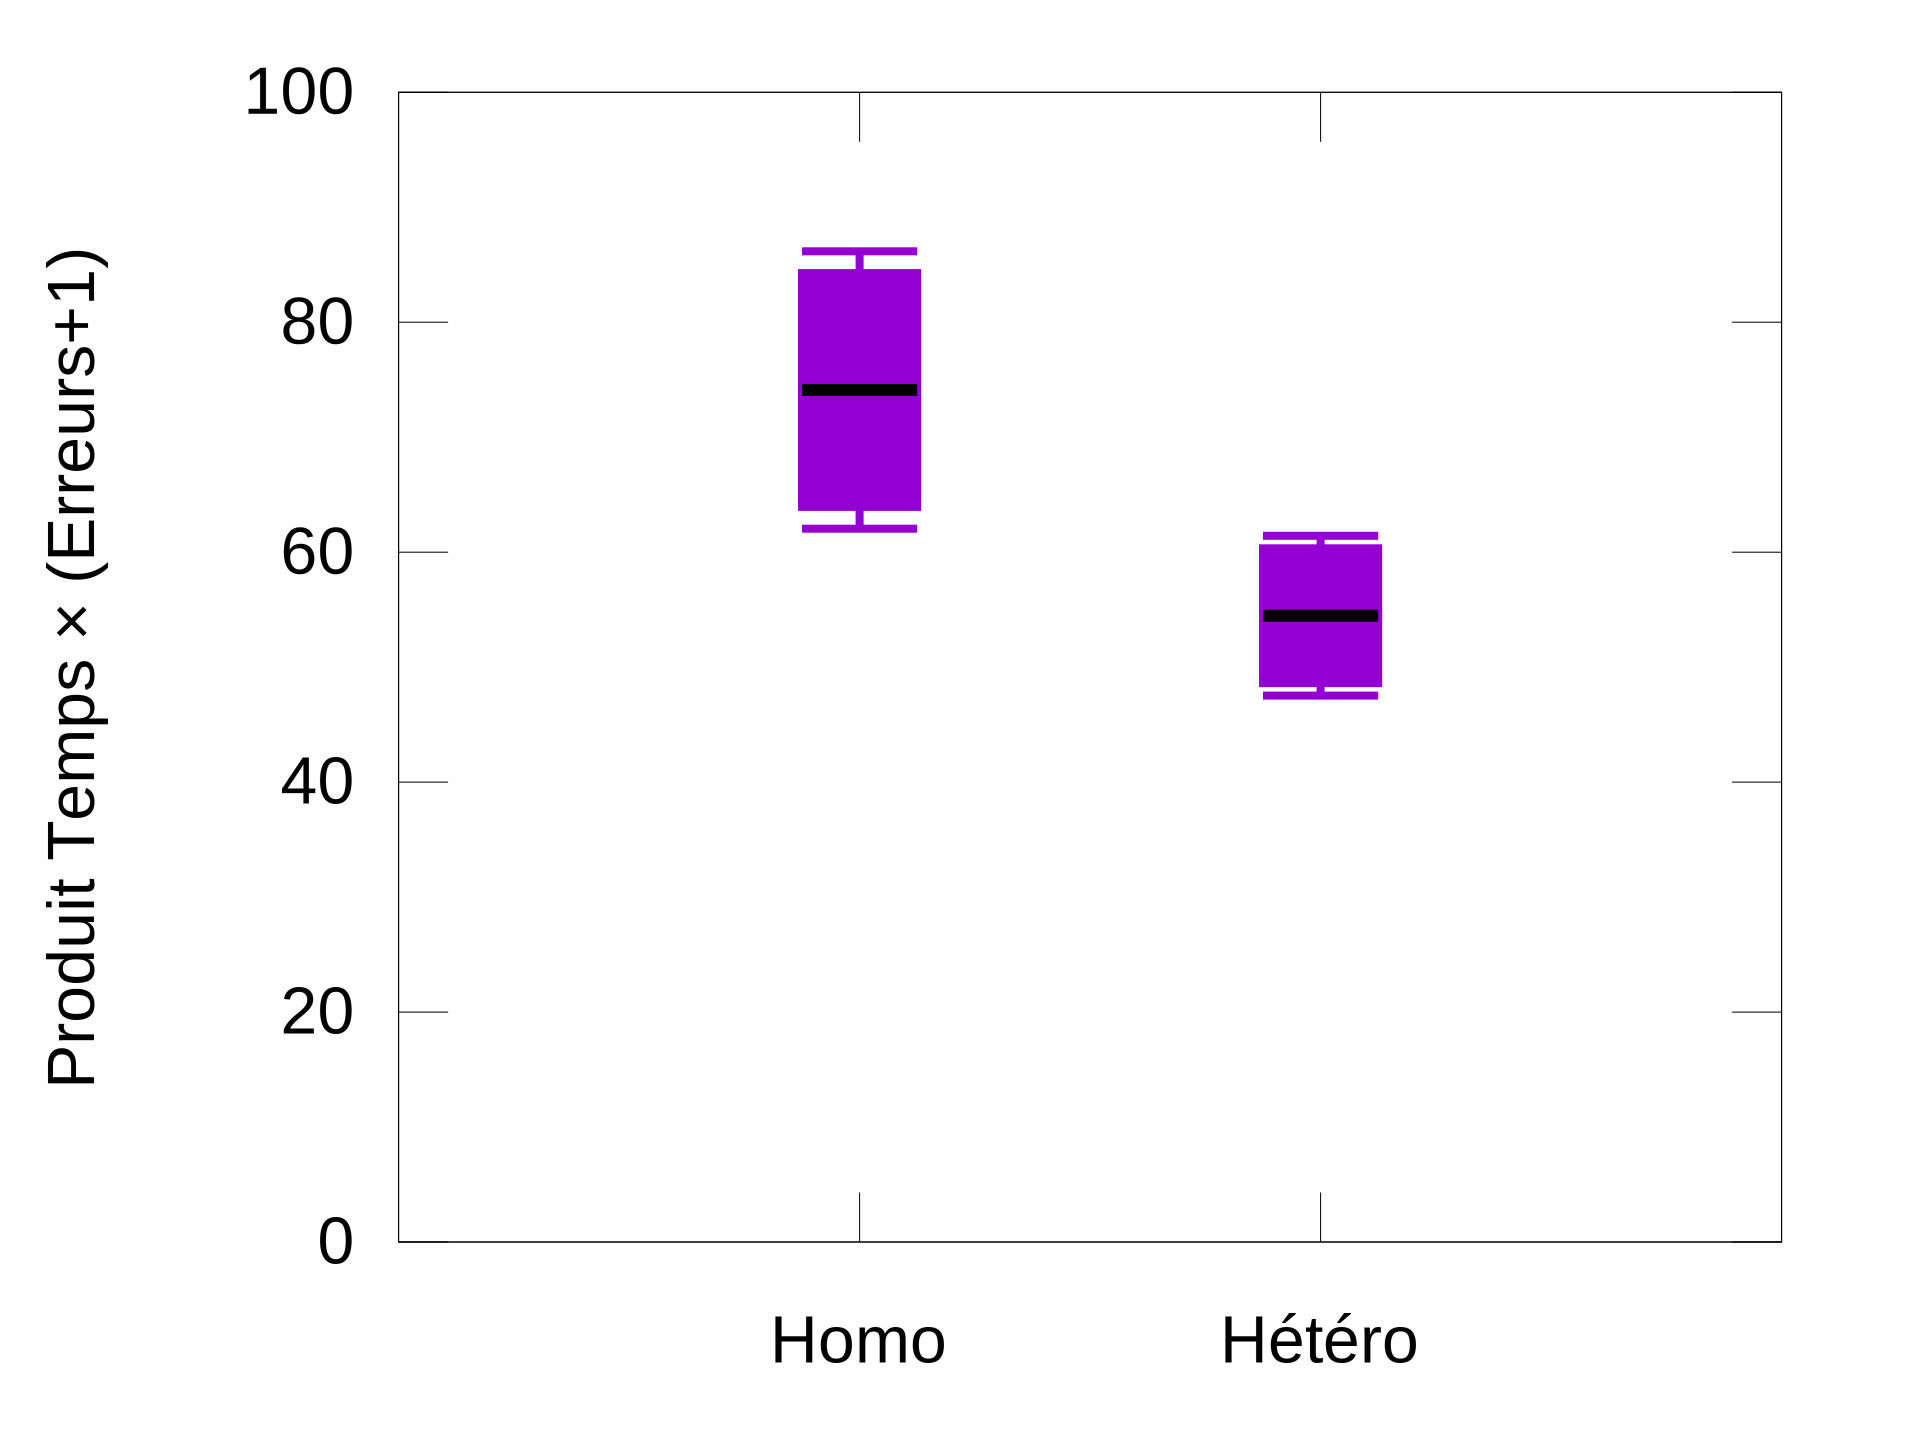
\includegraphics[width=\textwidth]{figures/ch5/productRes}
			\caption{$T(E+1)$. Les boîtes indiquent les IC à 95~\%{}, les \og moustaches \fg{} à leurs extrémités indiquent les IC à 98~\%{}, et les barres noires horizontales, les moyennes.}
			\label{fig:productRes}
		\end{subfigure}
		\caption[Temps et erreurs de sélection, homogène vs. hétérogène]{Temps et erreurs de sélection, en condition homogène et en condition hétérogène. IC = Intervalles de confiance.}
		\label{fig:timeAndErrorRes}
	\end{figure}
	
	\subsubsection{Temps de sélection}
	Dans la condition homogène, aucune corrélation significative ne fut trouvée entre le temps de sélection d'une cible et son paramètre F, ou A, comme nous pouvions nous y attendre compte tenu des interactions complexes entre les paramètres VFA.
	
	Cependant, une corrélation de 27,22~\%{} est observée entre la vitesse d'une cible et son temps de sélection, avec une \emph{p-value} de $2,19.10^{-43}$, ce qui n'est pas négligeable. Ces données confirment que la vitesse peut fournir une première approximation très grossière, mais potentiellement utile, de la difficulté de sélection d'une cible, ce qui est cohérent avec de nombreux travaux antérieurs. Mais une corrélation nettement plus forte est observée entre notre estimation de la difficulté de sélection d'une cible et son temps de sélection : 40,3~\%{}, avec une \emph{p-value} de $1,81.10^{-97}$. Notre hypothèse \textbf{H1} est donc retenue pour les temps de sélection.
	
	Il est par ailleurs intéressant d'observer que la corrélation entre la difficulté estimée et le temps de sélection est très fortement atténuée (et même inversée) dans la condition hétérogène : -7,13~\%{}, avec une \emph{p-value} inférieure à 0,0004. Ce résultat suggère que notre ajustement des tailles des cibles compense bien les écarts de difficulté\ldots{} et même un peu trop. La valeur du paramètre N choisie pour notre parabole était donc peut-être un peu trop élevée.
	
	La figure~\ref{fig:timeRes} présente les temps moyens de sélection observés dans la condition homogène d'une part, et hétérogène d'autre part. Si l'ajustement de la taille des cibles permet de diminuer le temps moyen de sélection, les intervalles de confiance à 95~\%{} se recoupent nettement ; aussi ne pouvons-nous retenir l'hypothèse \textbf{H2} pour les temps de sélection.
	
	\subsubsection{Erreurs}
	De même que pour les temps de sélection, dans la condition homogène, aucune corrélation significative n'est observé entre les erreurs et F ou A. En revanche, la corrélation entre la vitesse d'une cible et le nombre d'erreurs lors de sa sélection est relativement élevée : 29,95~\%{}, avec une \emph{p-value} de $1,46.10^{-52}$. Mais encore une fois, notre estimation de la difficulté fournit une meilleure corrélation : 43,02~\%{}, avec une \emph{p-value} de $2,72.10^{-112}$. Ici encore, nous observons une inversion de la corrélation dans la conditon hétérogène : -7,21~\%{}, avec une \emph{p-value} de 0,0003. Notre hypothèse \textbf{H1} est donc tout aussi valable pour les erreurs que pour les temps de sélection.
	
	La figure~\ref{fig:errorRes} présente le nombre moyen d'erreurs en fonction de la condition, homogène ou hétérogène. Là encore, si l'ajustement de la taille des cibles permet de diminuer le nombre moyen d'erreurs, les intervalles de confiance à 95~\%{} se chevauchent fortement, de sorte que nous ne pouvons retenir l'hypothèse \textbf{H2} pour les erreurs.
	
	\subsubsection{Performances de sélection}
	\label{sub:product}
	Néanmoins, les performances de sélection ne sauraient être envisagées sous l'angle seul des temps de sélection, ou des erreurs. En effet, les tâches physiques en général~\cite{woodworth1899accuracy}, et le pointage en particulier~\cite{fitts1966cognitive} sont connus depuis longtemps pour être des compromis entre vitesse et précision. Ce compromis est même quantifié pour le pointage~\cite{mackenzie2008fitts, guiard2011fitt, guiard2015mathematical}, et décrit comme un compromis de type \emph{max-max} si l'on considère la vitesse et la précision, qu'il faut maximiser, ou \emph{min-min} si l'on considère, de manière équivalente, le temps de sélection et les erreurs, qu'il faut minimiser.
	
	Nous proposons donc de considérer les deux valeurs \emph{simultanément}, plutôt que séparément. C'est l'objet de la figure~\ref{fig:errorsTimesScatter}, qui présente le nombre moyen d'erreurs en abscisse, et le temps moyen de sélection en ordonnée, pour chaque condition. Le but d'une technique d'aide à la sélection peut ainsi être conçu comme le déplacement des mesures de performance vers le coin inférieur gauche, idéalement sur les deux axes. C'est ce que l'ajustement des tailles des cibles permet, quoique de manière assez faible sur chaque axe.
	
	Observons au passage que les temps de sélection et les erreurs sont naturellement très fortement corrélés, à hauteur de 90,74~\%{} dans la condition homogène, et 86,82~\%{} dans la condition hétérogène ; dans les deux cas, la \emph{p-value} est trop faible pour que nos outils puissent la distinguer de zéro. Ainsi, l'ajustement des tailles ne change pas fondamentalement la nature du compromis vitesse-précision de la tâche.
	
	\paragraph{Produit temps $\times$ erreurs.}
	Il y a de surcroît un problème inhérent à l'examen du seul temps de sélection dans les études que nous présentons ici, puisque pour un essai donné, il peut y avoir un nombre non borné d'erreurs. De fait, un essai ayant pris 4 secondes avec aucune erreur, par exemple, n'est pas directement comparable à un autre essai ayant pris le même temps mais avec 15 erreurs. On peut en effet supposer que si le sujet avait veillé à ne commetre aucune erreur dans le second cas, il aurait mis bien plus de temps à sélectionner sa cible ; inversement, dans le premier cas, en étant moins prudent et en s'autorisant d'éventuelles erreurs, il aurait pu compléter sa sélection plus rapidement. De plus, dans une application réelle, une erreur peut avoir un \og coût \fg{} temporel additionnel, par exemple s'il faut désélectionner ce qui a été sélectionné par erreur, annuler une éventuelle action involontairement déclenchée par le clic erroné, ou si ce dernier a déclenché un retour graphique perturbant, etc.
	
	Par conséquent, et attendu que chaque composante des performances de sélection est à minimiser, nous pouvons adopter une métrique scalaire unique pour mesurer les performances : la moyenne des produits du temps de sélection par le nombre d'erreurs, pour chaque essai. Afin d'éviter d'obtenir des résultats nuls en cas d'absence d'erreur, et pour conserver le temps de sélection tel quel dans ce cas-là, nous proposons la métrique suivante : $Perf = T \times{} (E+1)$, où $Perf$ représente les performances, $T$ est le temps de sélection, et $E$ le nombre d'erreurs.
	
	Assez logiquement, il n'y a pas de corrélation significative entre $Perf$ et F, ou A, mais il y en a une entre $Perf$ et V : 19,80~\%{}, avec une \emph{p-value} de $2,39.10^{-23}$, et surtout entre $Perf$ et l'estimation de la difficulté de la cible : 29,35~\%{}, avec une \emph{p-value} de $1,77.10^{-50}$. Nous avons calculé cette valeur pour chaque essai, et en présentons les moyennes dans la figure~\ref{fig:productRes}, avec les intervalles de confiance à 95~\%{} et 98~\%{}, qui demeurent disjoints entre les conditions homogène et hétérogène, avec un net avantage pour cette dernière.
	
	Il nous apparaît donc que, sur le fondement de cette métrique de performances, inspirée des travaux sur le compromis vitesse-précision exprimé par la loi de Fitts, notre hypothèse \textbf{H2} peut être retenue, concernant les performances de sélection prises dans leur ensemble.
	
	\subsubsection{Homogénéisation des performances}
	Notre ajustement des tailles des objets mobiles ayant pour conséquence de faciliter la sélection des cibles difficile, et de rendre plus difficile la sélection des cibles faciles, il est possible de voir le procédé comme une homogénéisation des performances de sélection sur l'ensemble des cibles en présence. Dans certains types d'application, garantir (ou favoriser) une expérience d'utilisateur homogène selon les conditions rencontrées peut être vu comme une fin en soi.
	
	De fait, il est intéressant de chercher à quantifier cette homogénéisation des performances de sélection. C'est ce que fait la figure~\ref{fig:homogeneityHistogram}, qui présente les écarts-types du temps de sélection, du nombre d'erreurs, et de $Perf$, selon la condition. Sur toutes ces métriques, l'ajustement des tailles des cibles est corrélé avec une diminution, assez marquée sur les erreurs, très marquée sur $Perf$.

	\begin{figure}[!htb]
		\begin{subfigure}[t]{0.49\textwidth}
			\centering
			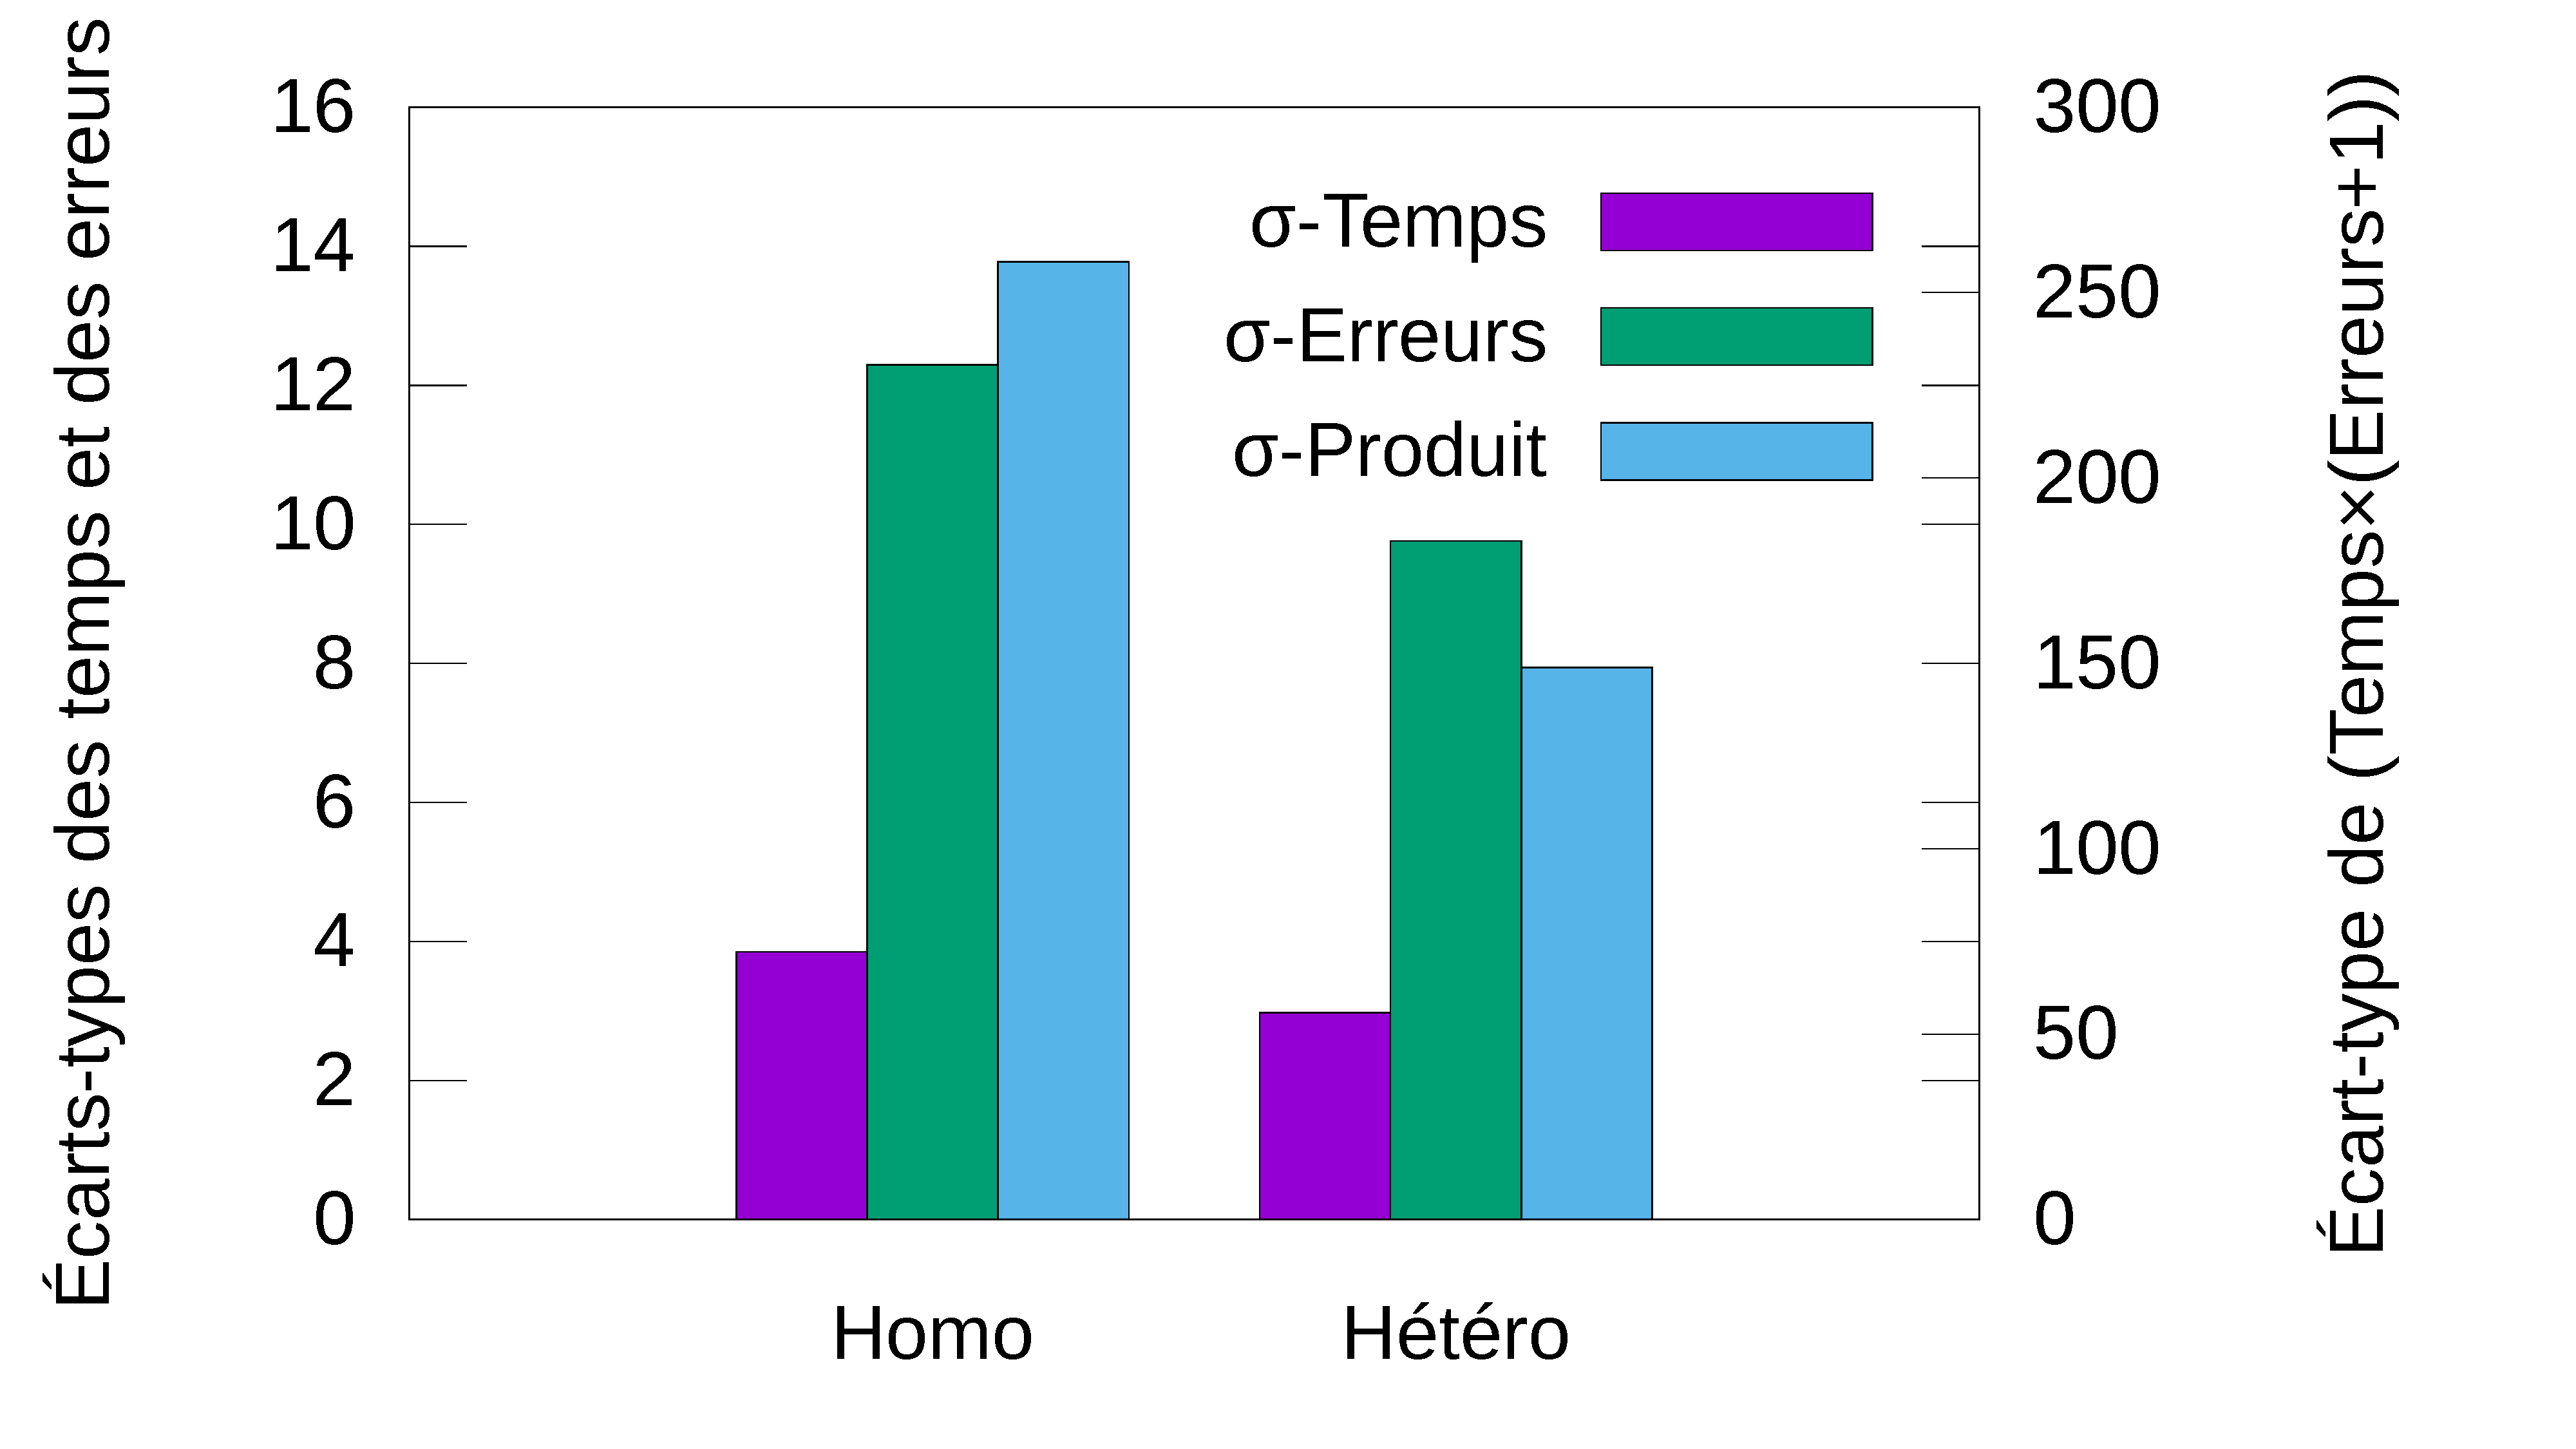
\includegraphics[width=\textwidth]{figures/ch5/homogeneityHistogram}
			\caption{Résultats bruts.}
			\label{fig:homogeneityHistogram}
		\end{subfigure}
		~
		\begin{subfigure}[t]{0.49\textwidth}
			\centering
			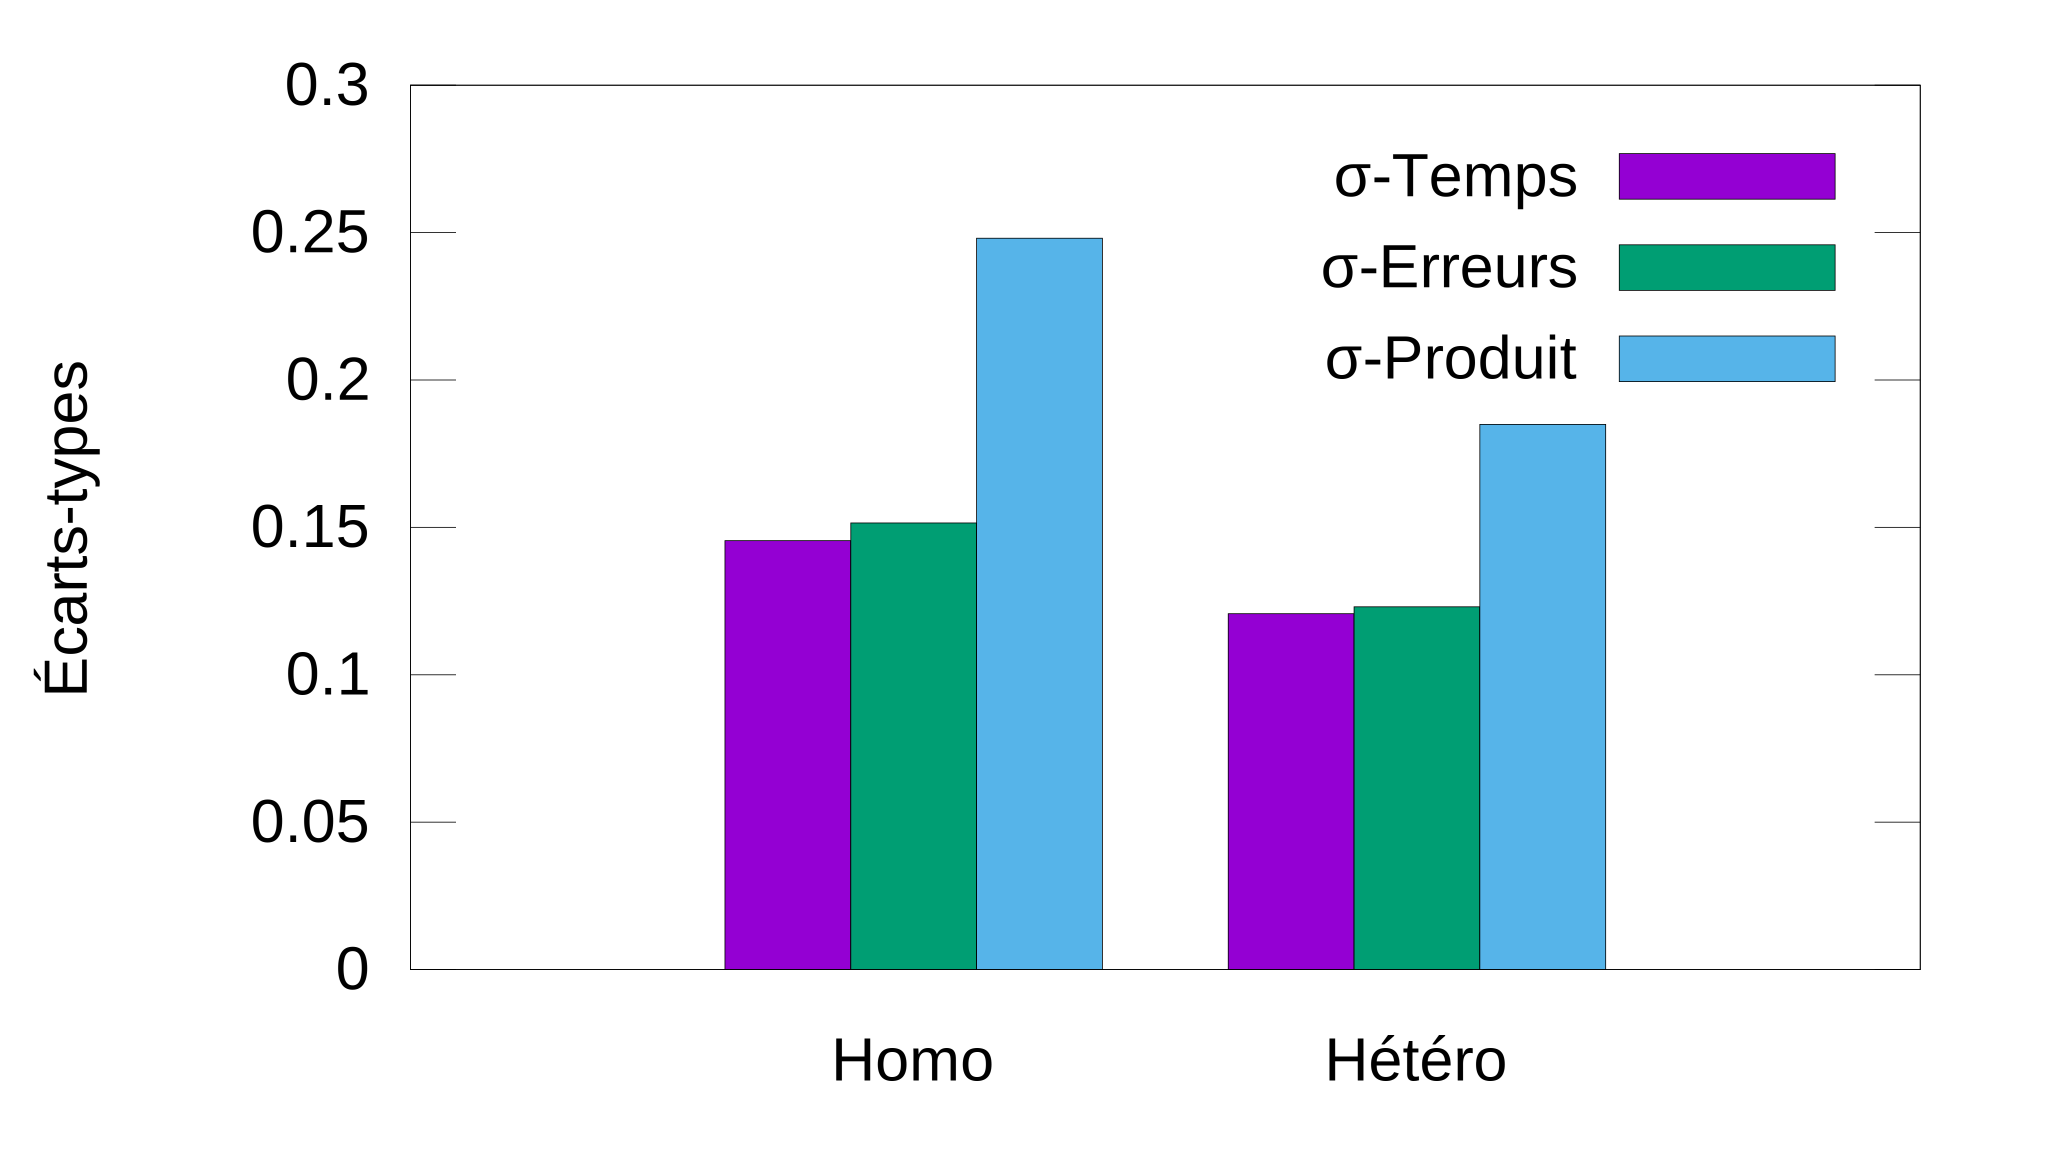
\includegraphics[width=\textwidth]{figures/ch5/normHomogeneityHistogram}
			\caption{Résultats normalisés.}
			\label{fig:normHomogeneityHistogram}
		\end{subfigure}
		\caption[Homogénéisation des performances]{Homogénéisation des performances par ajustement des tailles des cibles. Les écarts-type du temps de sélection, du nombre d'erreurs, et du produit $Perf$ sont représentés, cette dernière valeur étant sur l'échelle de droite dans la figure~\ref{fig:homogeneityHistogram}.}
		\label{fig:homoHistosNormAndRaw}
	\end{figure}
	
	\subsection{Normalisation des résultats}
	Comme nous l'expliquions dans le chapitre~\ref{chap4}, l'examen de moyennes sur des résultats bruts a l'inconvénient de donner plus de poids aux sujets relativement lents. C'est un choix possible pour l'évaluation d'une technique de sélection, si l'on considère qu'il convient de se concentrer sur les individus ayant le plus de difficultés à accomplir une tâche. C'est pourquoi nous avons présenté nos résultats bruts. Le fait d'étudier les résultats bruts a également l'inconvénient de masquer quelque peu les corrélations entre la nature des mouvements d'une combinaison VFA et les performances de sélection qui y sont associées, puisque celles-ci sont \og bruitées \fg{} par les différences entre les sujets.
	
	Mais une méthode plus égalitaire et plus propice à l'étude des corrélations consiste à normaliser les résultats, par exemple en divisant, pour chaque sujet, tous ses temps de sélection par son temps le plus long, et tous ses taux d'erreurs par son taux d'erreurs le plus élevé. C'est ce que nous avons faits, et les résultats correspondants sont fournis dans la figure~\ref{fig:normAsTimeAndErrors}. Une fois normalisés, les résultats indiquent un avantage plus faible pour la condition hétérogène, mais toujours présent, et relativement clair sur la métrique $Perf$ (figure~\ref{fig:normAsProducts}. La diminution du phénomène avec normalisation suggère qu'il est moins marqué chez les sujets rapides. La normalisation permet néanmoins de mettre en lumière une plus forte corrélation entre $Perf$ et notre estimation de la difficulté en condition homogène, comme le rapporte le tableau~\ref{tab:synthRes}. Ceci conforte à nouveau notre hypothèse \textbf{H1}.
	

	\begin{figure}[!htb]
		%\centering
		\begin{subfigure}[t]{0.49\textwidth}
			\centering
			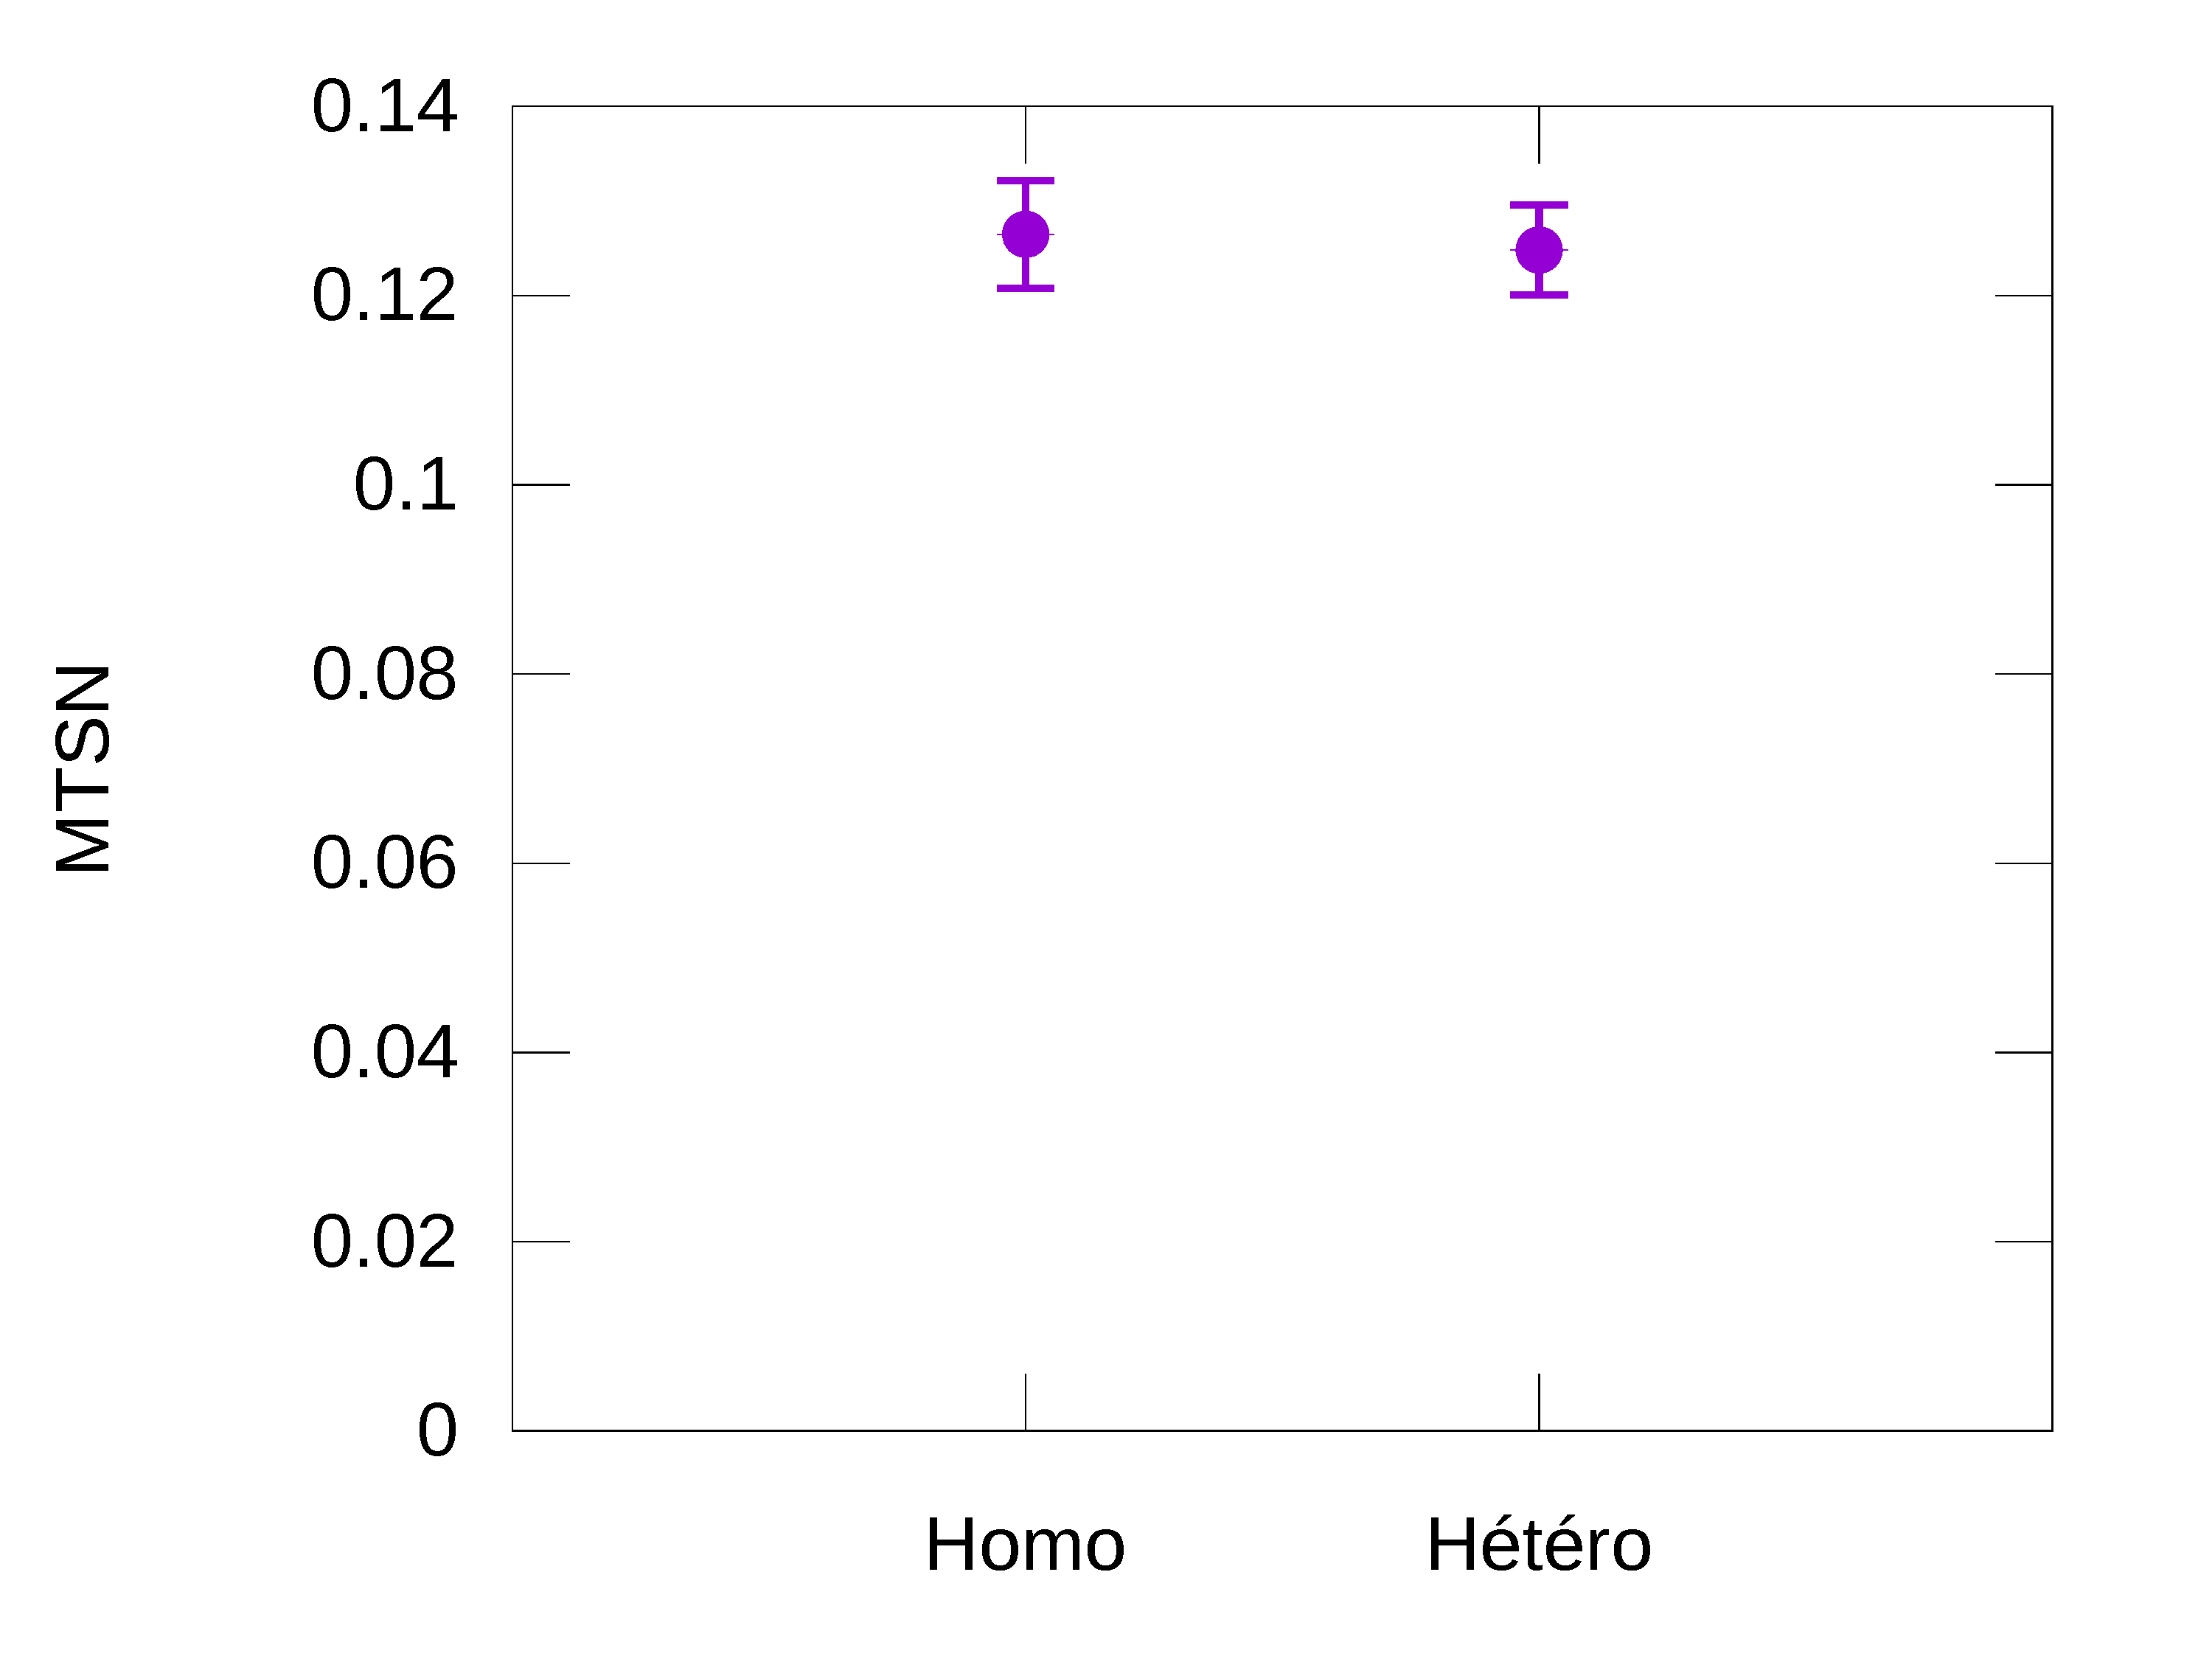
\includegraphics[width=\textwidth]{figures/ch5/normAsTimes}
			\caption{MTSN.}
			\label{fig:normAsTimes}
		\end{subfigure}
		~
		\begin{subfigure}[t]{0.49\textwidth}
			\centering
			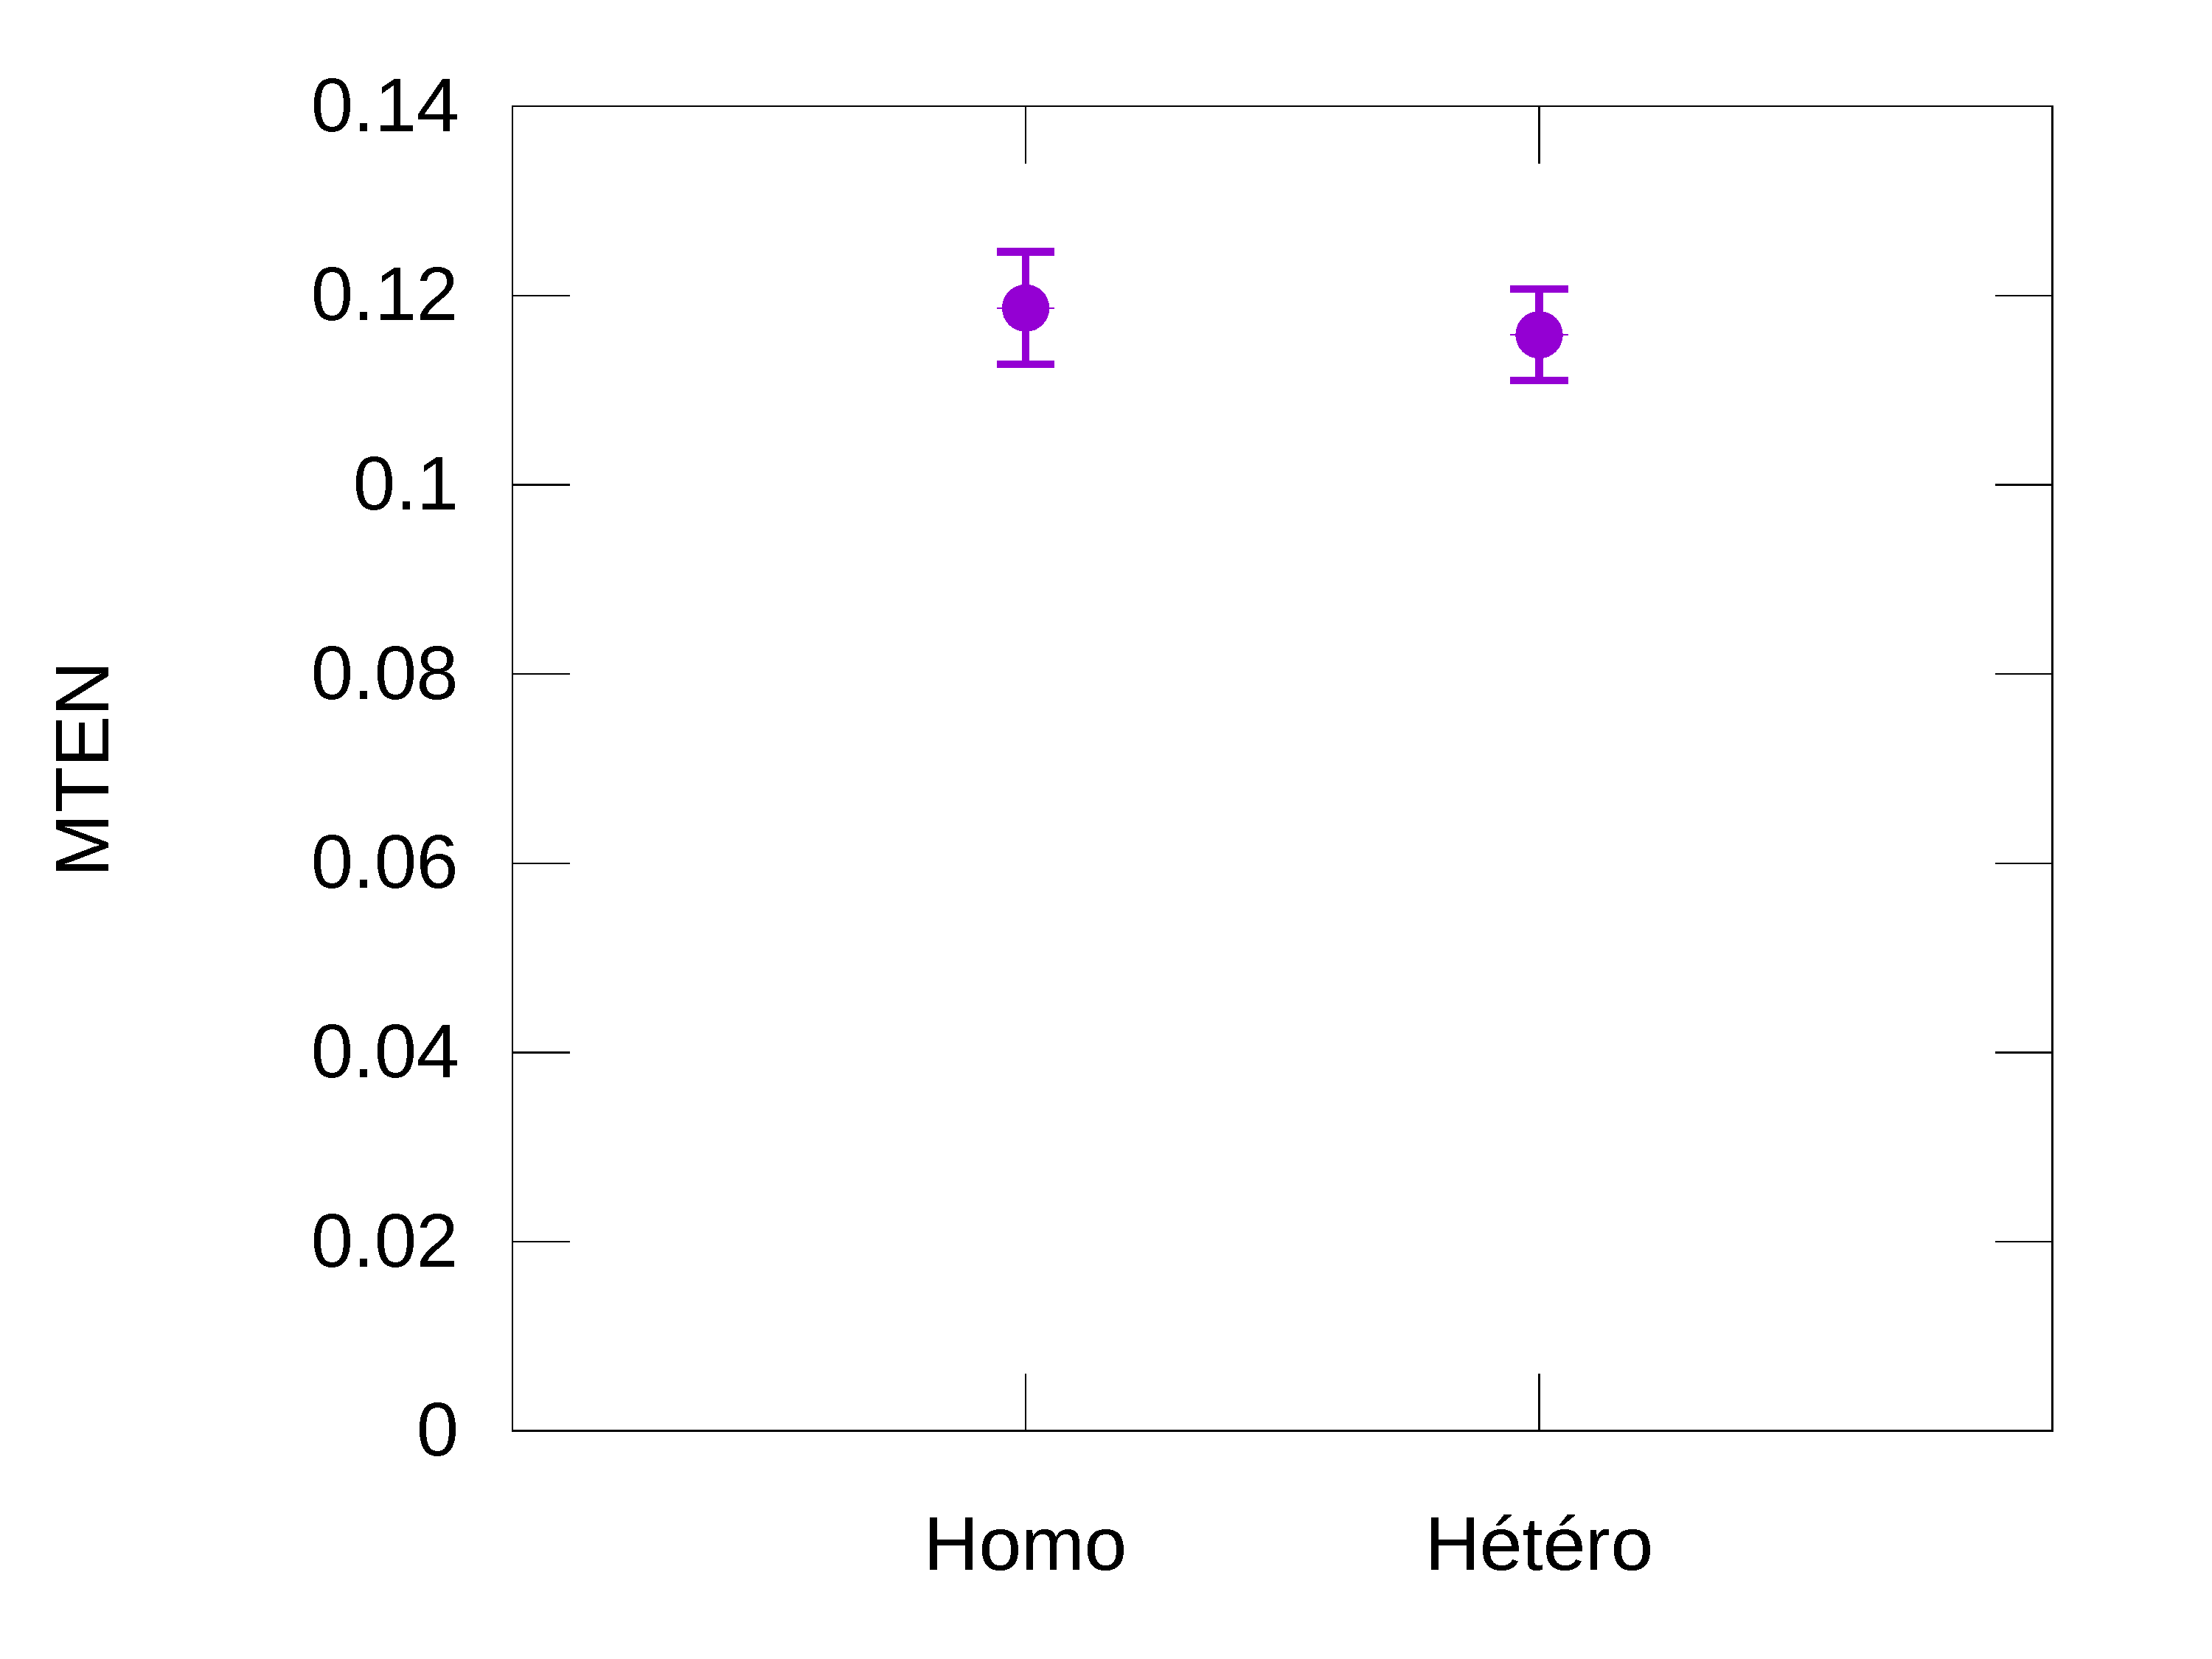
\includegraphics[width=\textwidth]{figures/ch5/normAsErrors}
			\caption{MTEN.}
			\label{fig:normAsErrors}
		\end{subfigure}
		~
		\begin{subfigure}[t]{0.49\textwidth}
			\centering
			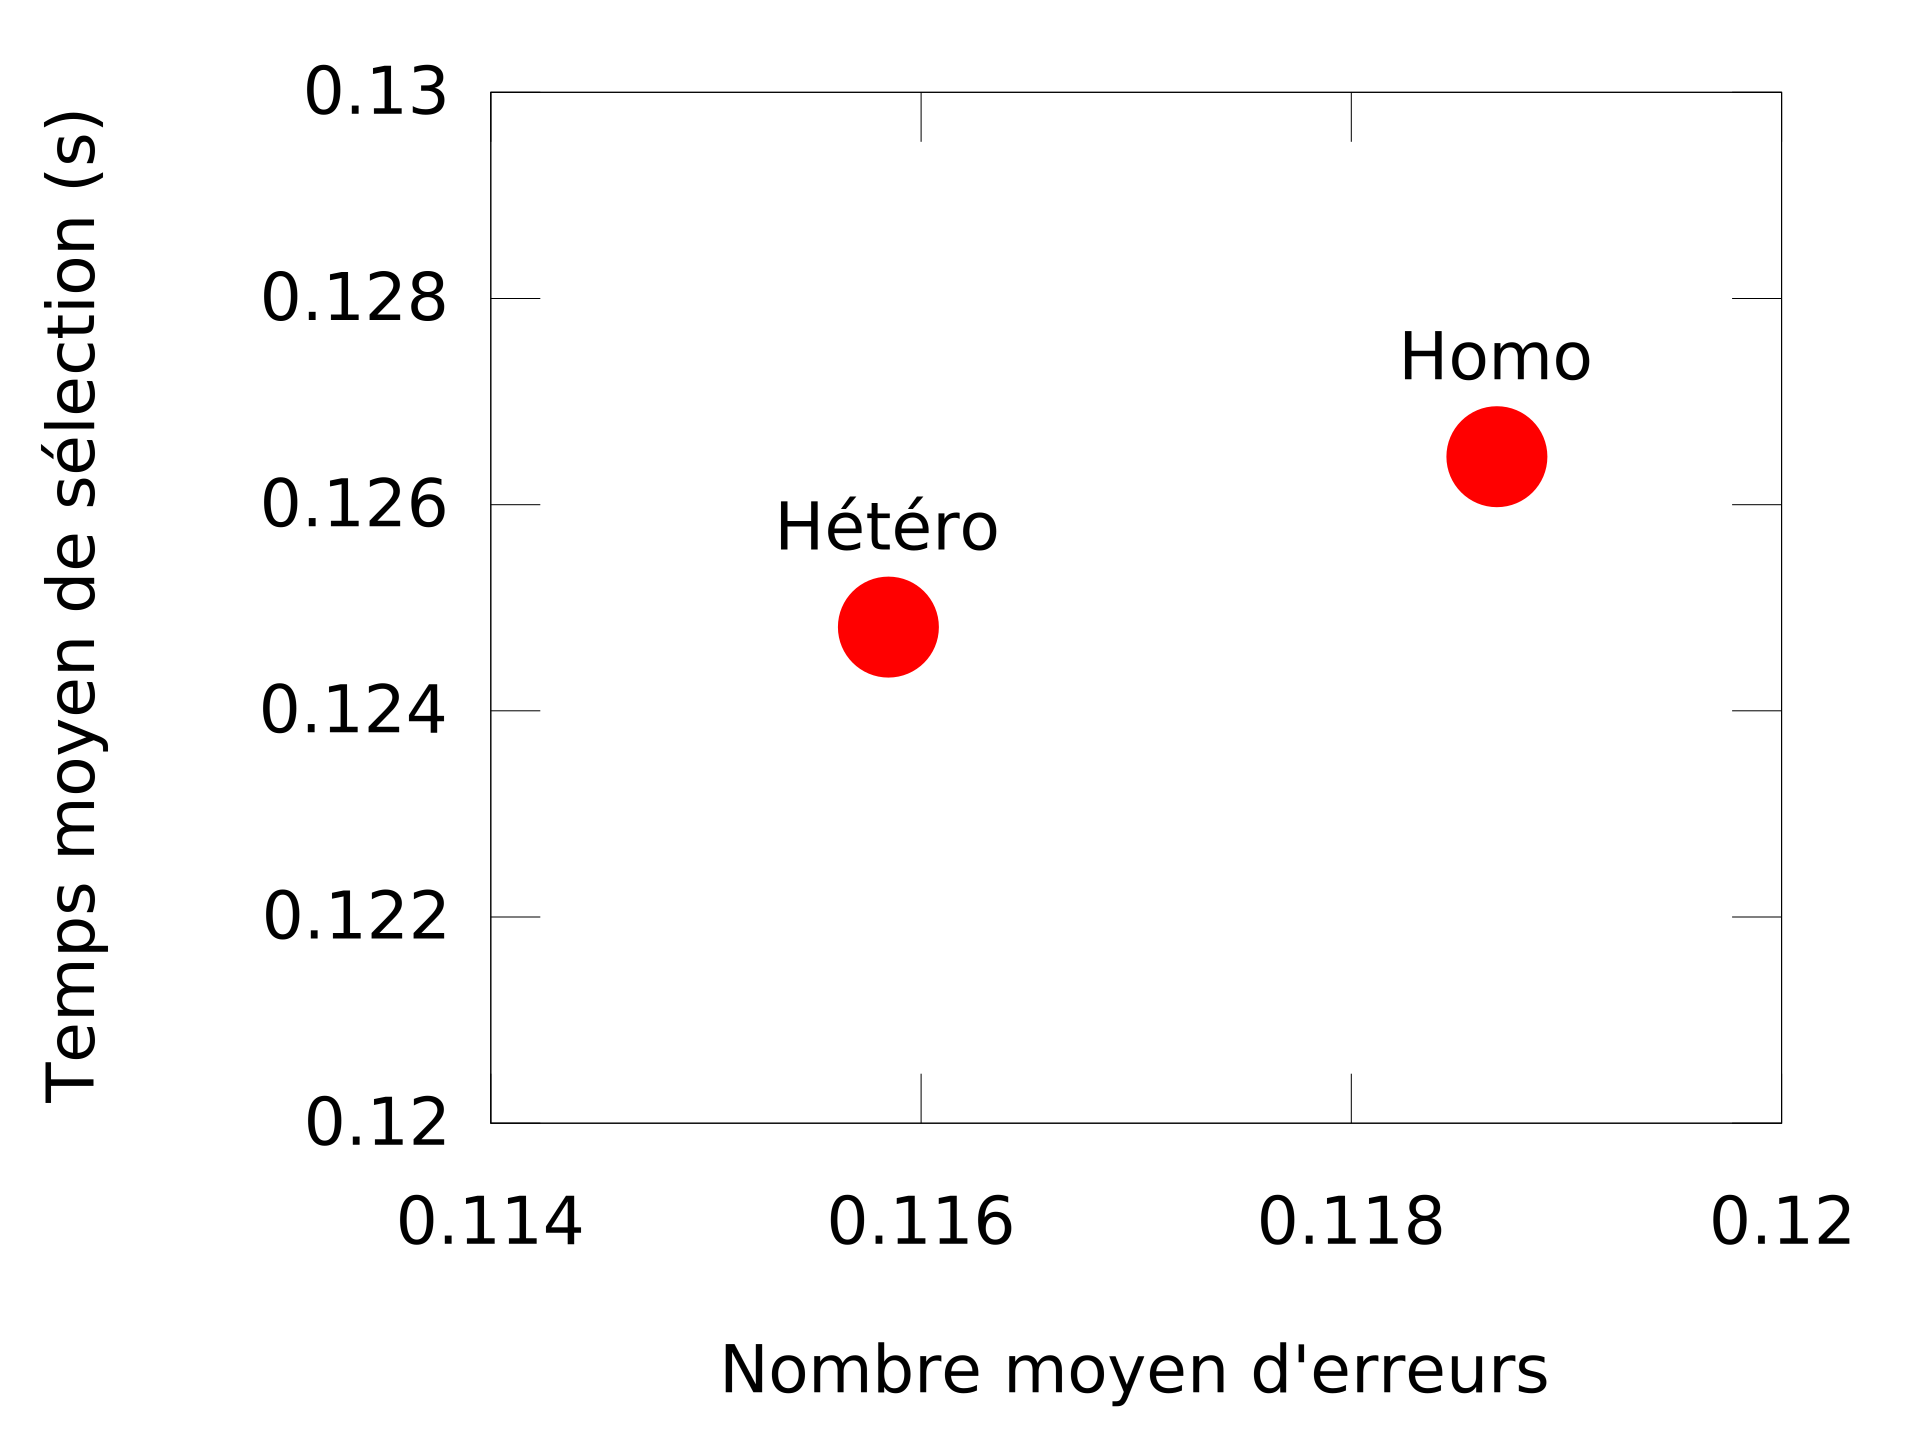
\includegraphics[width=\textwidth]{figures/ch5/normErrorsTimesScatter}
			\caption{MTSN et MTEN.}
			\label{fig:normErrorsTimesScatter}
		\end{subfigure}
		~
		\begin{subfigure}[t]{0.49\textwidth}
			\centering
			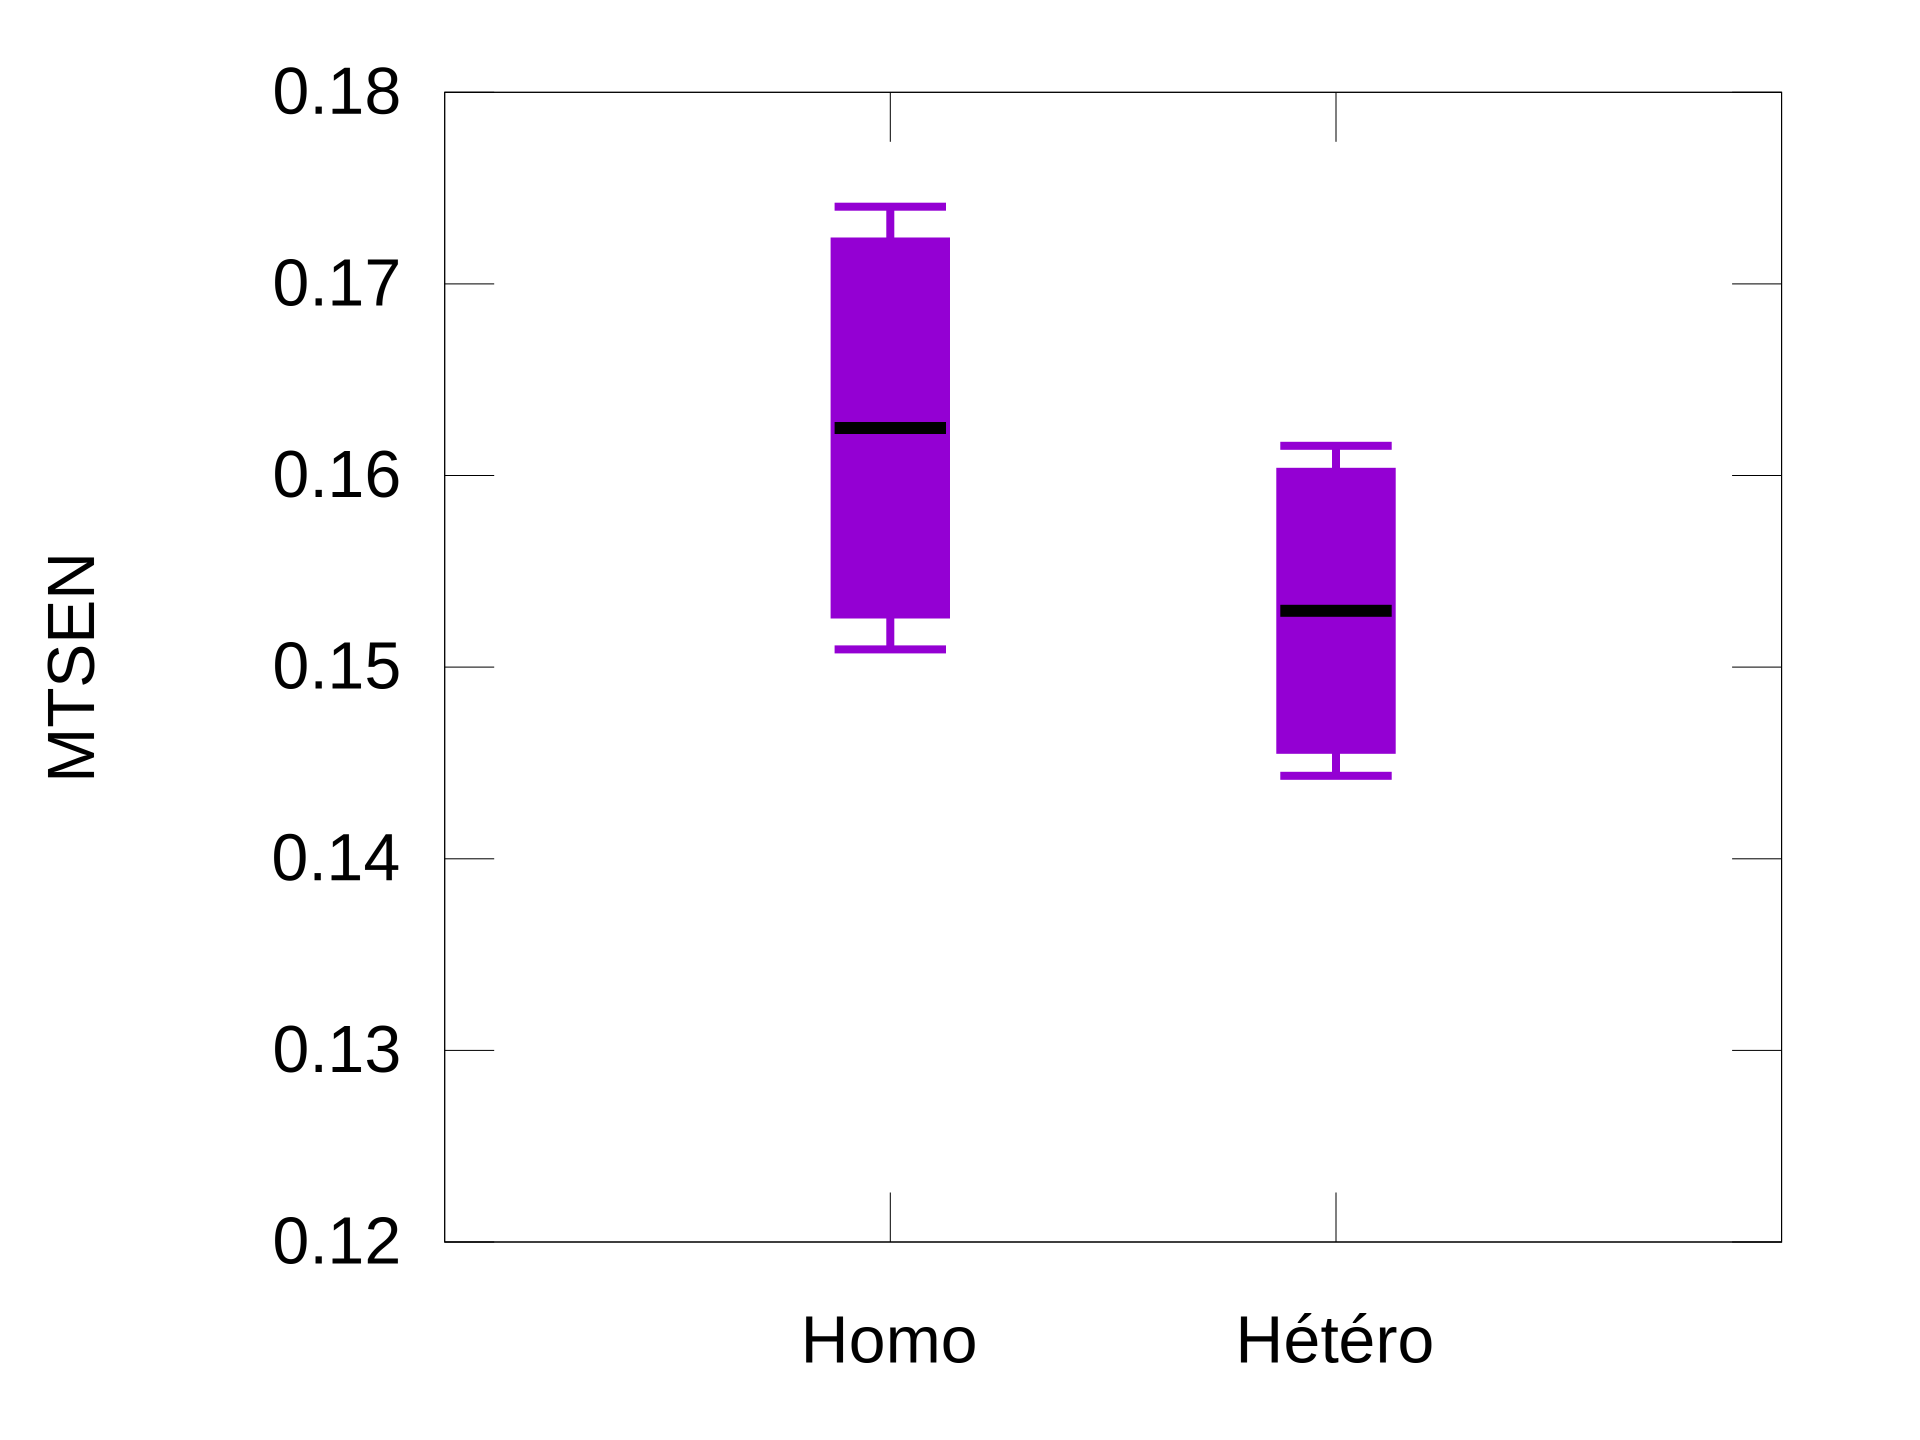
\includegraphics[width=\textwidth]{figures/ch5/normAsProducts}
			\caption{$\overline{Perf}$ (avec normalisation). Boîtes : IC à 95~\%{} ; \og moustaches \fg{} : IC à 98~\%{} ; barres noires : moyennes.}
			\label{fig:normAsProducts}
		\end{subfigure}
		\caption[Temps et erreurs de sélection, homogène vs. hétérogène -- II]{Temps et erreurs de sélection, en condition homogène et en condition hétérogène, normalisés.}
		\label{fig:normAsTimeAndErrors}
	\end{figure}


	\subsection{Synthèse des résultats}
	Nous proposons dans le tableau~\ref{tab:synthRes} une synthèse des résultats numériques de notre étude sur l'ajustement des tailles des cibles. Les valeurs de ce tableau correspondent à celles présentées graphiquement dans les sections précédentes.
	
%	\newcommand{\newrow}{\bigstrut[t] \\ \hline}
\begin{table}
	\centering
	\begin{tabular}{l | c c c c}
		Condition		& Homo						& Hétéro					& Homo (norm)				& Hétéro (norm)				\bigstrut[b] \\ \hline
		$\overline{T}$	& 2,98						& 2,84						& 12,65						& 12,48						\bigstrut[t] \\
		IC 95~\%{}		& [2,82 ; 3,13]				& [2,73 ; 2,96]				& [12,08 ; 13,22]			& [12,01 ; 12,95]			\bigstrut[b] \\ \hline
		$\overline{E}$	& 9,48						& 9,30						& 11,87						& 11,58						\bigstrut[t] \\
		IC 95~\%{}		& [9,00 ; 9,96]				& [8,92 ; 9,69]				& [11,27 ; 12,46]			& [11,10 ; 12,07]			\bigstrut[b] \\ \hline
		$\overline{P}$	& 73,84						& 54,32						& 16,25						& 15,29						\bigstrut[t] \\
		IC 95~\%{}		& [63,74 ; 83,94]			& [48,50 ; 60,14]			& [15,27 ; 17,22]			& [14,57 ; 16,02]			\\
		IC 98~\%{}		& [61,85 ; 85,82]			& [47,41 ; 61,23]			& [15,09 ; 17,40]			& [14,43 ; 16,16]			\bigstrut[b] \\ \hline
		C($d$, $T$)		& 40,16 ; 2$.10^{-97}$		& -7,10 ; 4$.10^{-4}$		& 42,59 ; 1$.10^{-110}$		& -9,11 ; 5$.10^{-6}$		\bigstrut[t] \\
		C(V, $T$)		& 27,12 ; 3$.10^{-43}$		& -5,21 ; 9$.10^{-3}$		& 29,27 ; 2$.10^{-50}$		& -6,72 ; 8$.10^{-4}$		\\
		C($d$, $E$)		& 42,89 ; 3$.10^{-112}$		& -7,20 ; 3$.10^{-4}$		& 42,68 ; 5$.10^{-111}$		& -7,75 ; 1$.10^{-4}$		\\
		C(V, $E$)		& 29,86 ; 2$.10^{-52}$		& -4,74 ; 0,02				& 29,83 ; 2$.10^{-52}$		& -5,30 ; 0,0081			\\
		C($d$, $P$)		& 29,28 ; 2$.10^{-50}$		& -3,77 ; 0,06				& 39,20 ; 2$.10^{-92}$		& -8,14 ; 5$.10^{-5}$		\\
		C(V, $P$)		& 19,74 ; 2$.10^{-23}$		& -3,04 ; 0,13				& 26,92 ; $10^{-42}$		& -6,21 ; 0,0019			\\
		C($T$, $E$)		& 90,73 ; --				& 0,8680 ; --				& 95,33						& 92,03						\\
		$\sigma{}T$		& 3,83						& 2,96						& 0,15						& 0,12						\\
		$\sigma{}E$		& 12,25						& 9,73						& 0,15						& 0,15						\\
		$\sigma{}P$		& 257,47					& 148,40					& 0,25						& 0,18						\\
	\end{tabular}
	\caption[Synthèse des résultats de l'étude sur l'ajustement des tailles]{Synthèse des résultats de l'étude sur l'ajustement des tailles. Les abbréviations \og IC \fg{}, \og C \fg{}, \og $d$ \fg{}, \og $T$ \fg{}, \og $E$ \fg{}, \og $P$ \fg{}, et \og norm \fg{}  signifient respectivement \og Intervalle de confiance à \fg{}, \og Corrélation \fg{} (accompagnée de sa \emph{p-value}), \og estimation de la difficulté de sélection d'une cible \fg{}, \og Temps \fg{}, \og Erreurs \fg{}, \og $Perf$ \fg{} et \og avec normalisation \fg{}. Un $\sigma$ indique un écart-type, et une barre horizontale, une moyenne. Les corrélations sont exprimées en pourcentages. Celles entre la vitesse ou l'estimation de la difficulté d'une part, et le temps de sélection, les erreurs, ou $Perf$ de l'autre, qui sont marquées et significatives dans la condition homogène, disparaissent --- et même s'inversent --- dans la condition hétérogène. La normalisation renforce les corrélations dans la condition homogène, particulièrement pour $Perf$.}
	\label{tab:synthRes}
\end{table}


	\subsection{Faibles vitesses de curseur}
	Comme précédemment, nous avons analysé les profils de vitesse du curseur. Les résultats sont tout à fait analogues à ce que nous avions observé dans le chapitre~\ref{chap4}, et la figure~\ref{fig:asProfiles} en fournit un exemple, avec les vitesses brutes d'une part, et lissées par moyenne mobile d'autre part. Au-delà de cet examen qualitatif, mais superficiel, nous avons examiné, pour chaque essai de sélection, la vitesse maximale du curseur, et la proportion de temps passé par le curseur en dessous de 25~\%{} de ce maximum. Nous avons ensuite calculé la moyenne géométrique de toutes ces proportions, toutes conditions et tous sujets confondus : elle est de 77,4~\%{} ; c'est-à-dire que pendant plus des trois quarts du temps, le curseur se déplace à moins d'un quart de sa vitesse maximale.
	
	Ces résultats sont à relier à nos observations sur la relative indépendance des performances de sélection par rapport à la distance de Fitts (section~\ref{sub:fittsDistance}). En effet, lorsque la sélection est difficile, les phases dites balistiques, pendant lesquelles le curseur se déplace rapidement pour se rapprocher de la cible, sont temporellement dominées par les phases de \og poursuite \fg{} de la cible, en moyenne beaucoup plus lentes, à l'exception de quelques à-coups. Ce sont les observations de ce type qui nous ont conduits à ajuster les tailles des cibles sans chercher à jouer sur les distances de Fitts, réelles ou effectives.	
	
	\begin{figure}[!htb]
		\begin{subfigure}[t]{\textwidth}
			\centering
			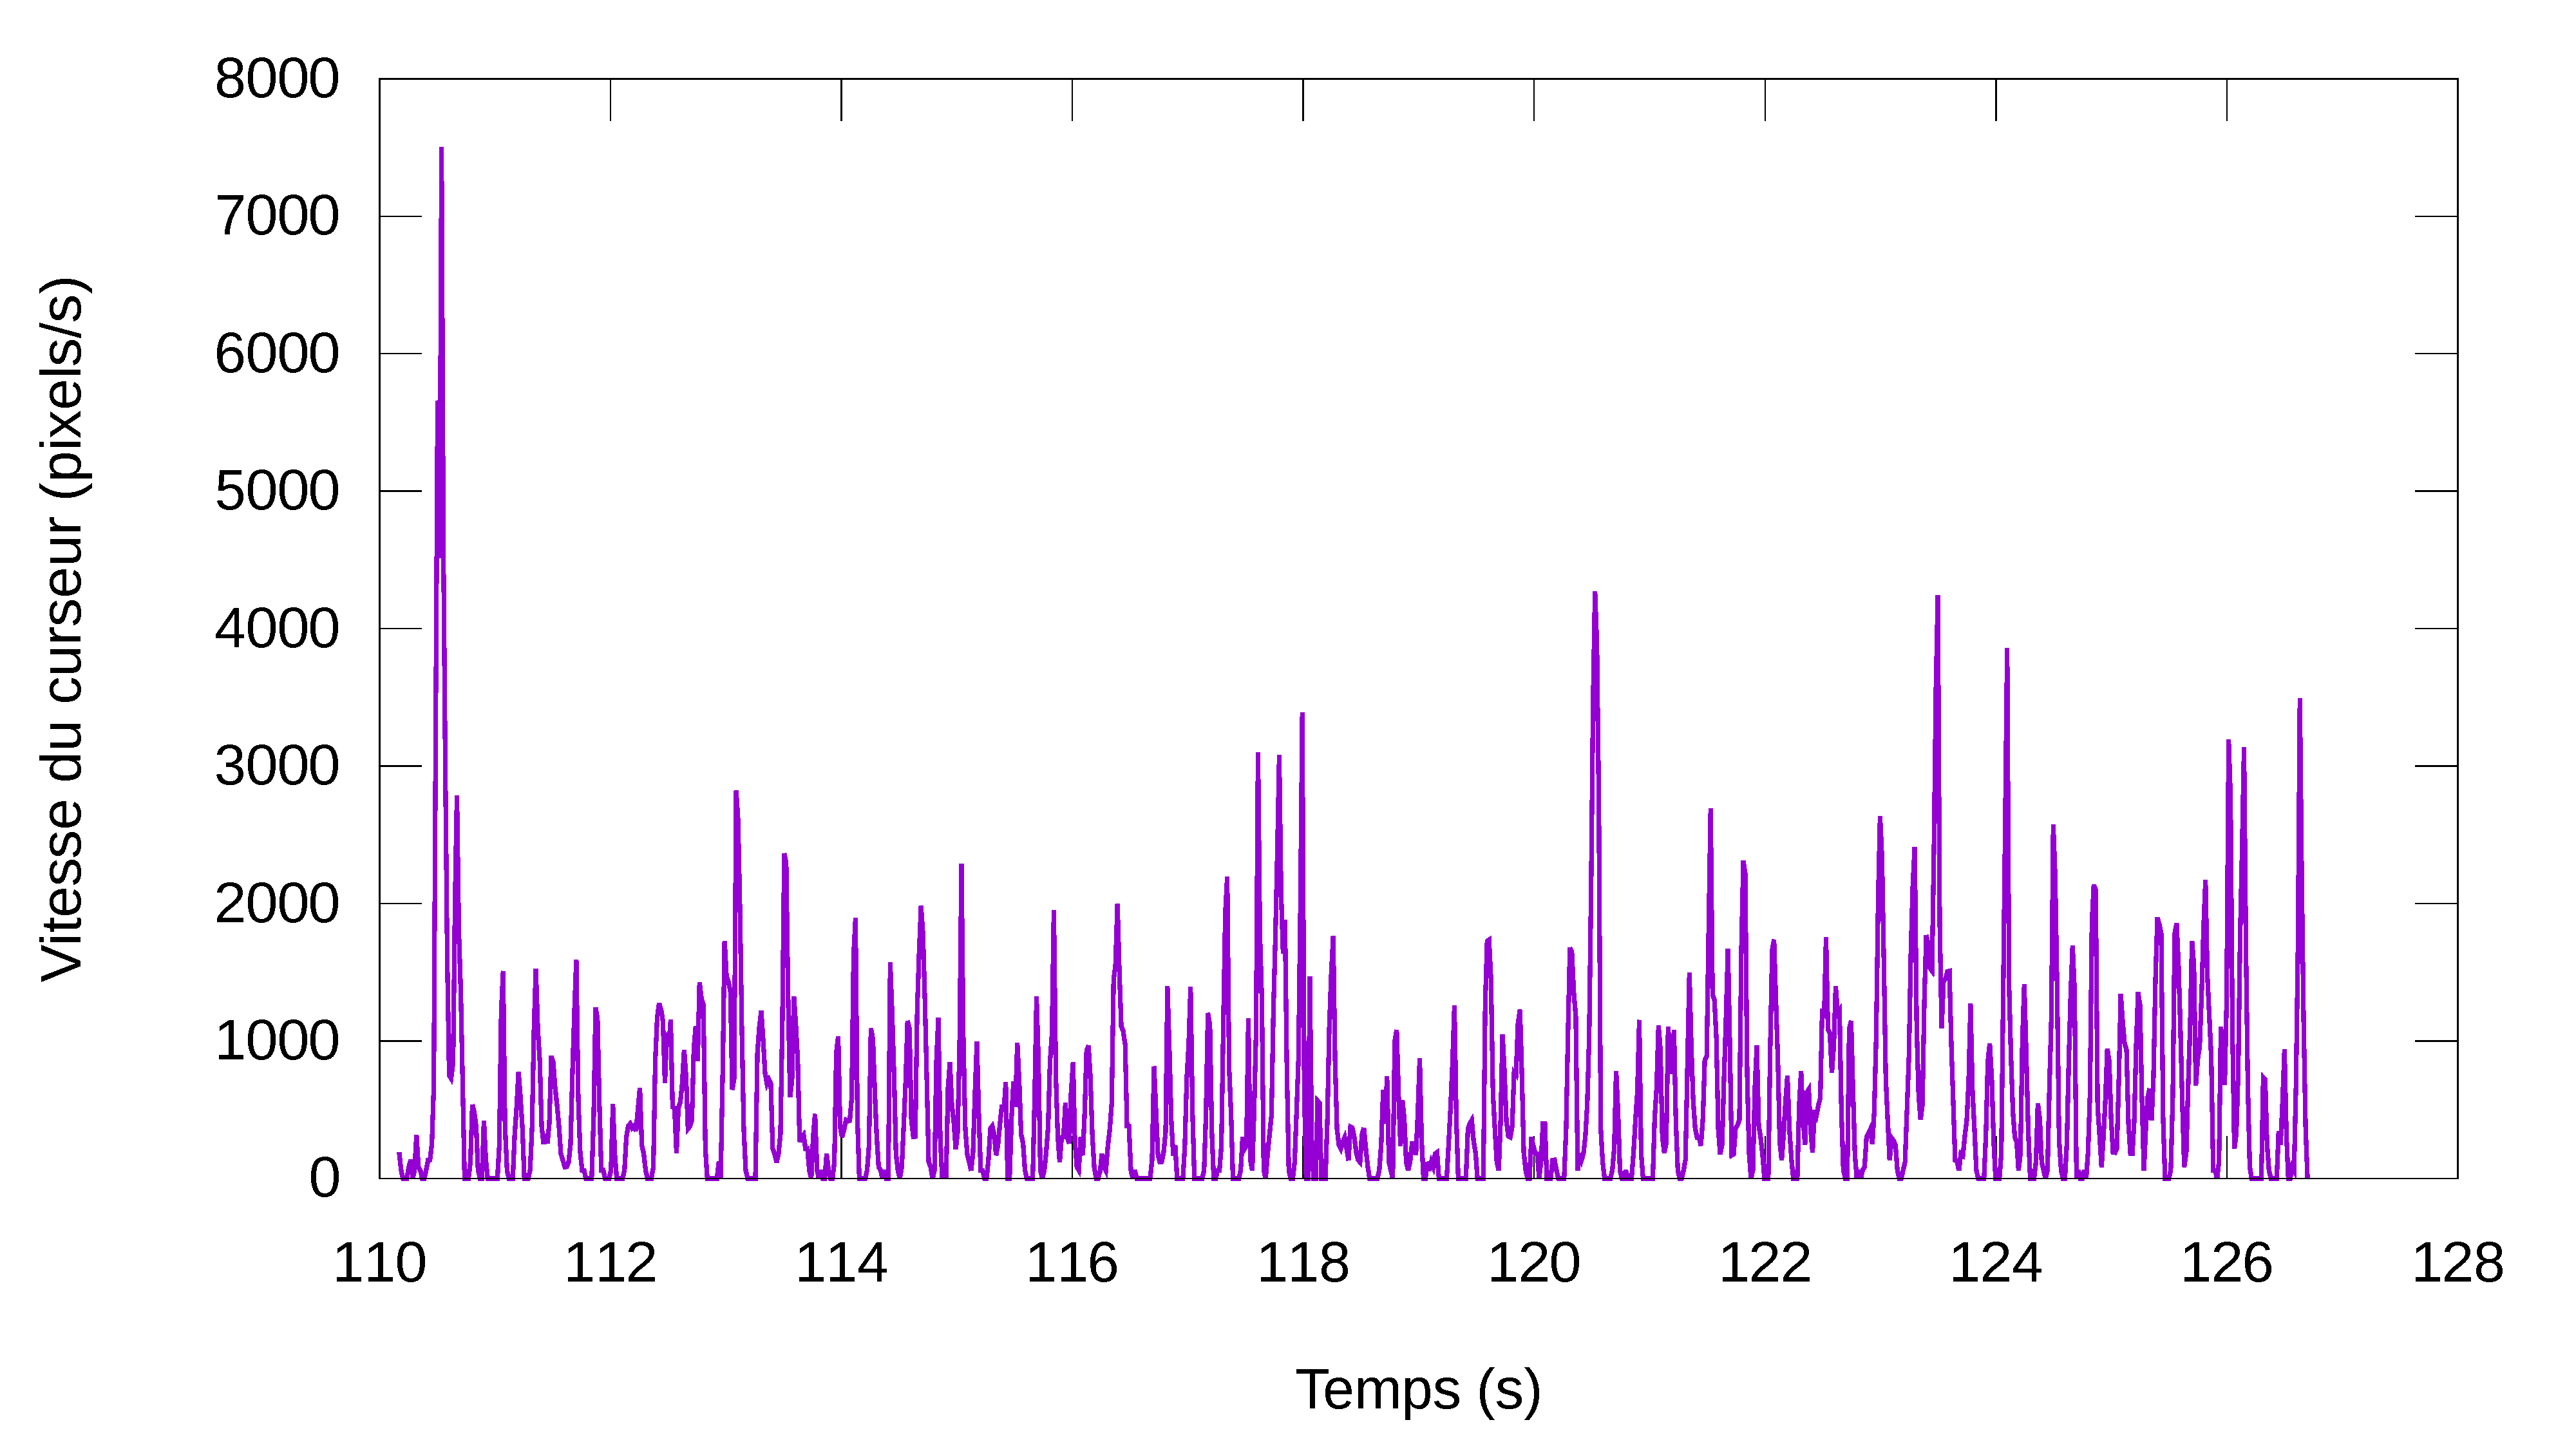
\includegraphics[width=\textwidth]{figures/ch5/profile}
			\caption{Résultats bruts.}
			\label{fig:profile}
		\end{subfigure}
		~
		\begin{subfigure}[t]{\textwidth}
			\centering
			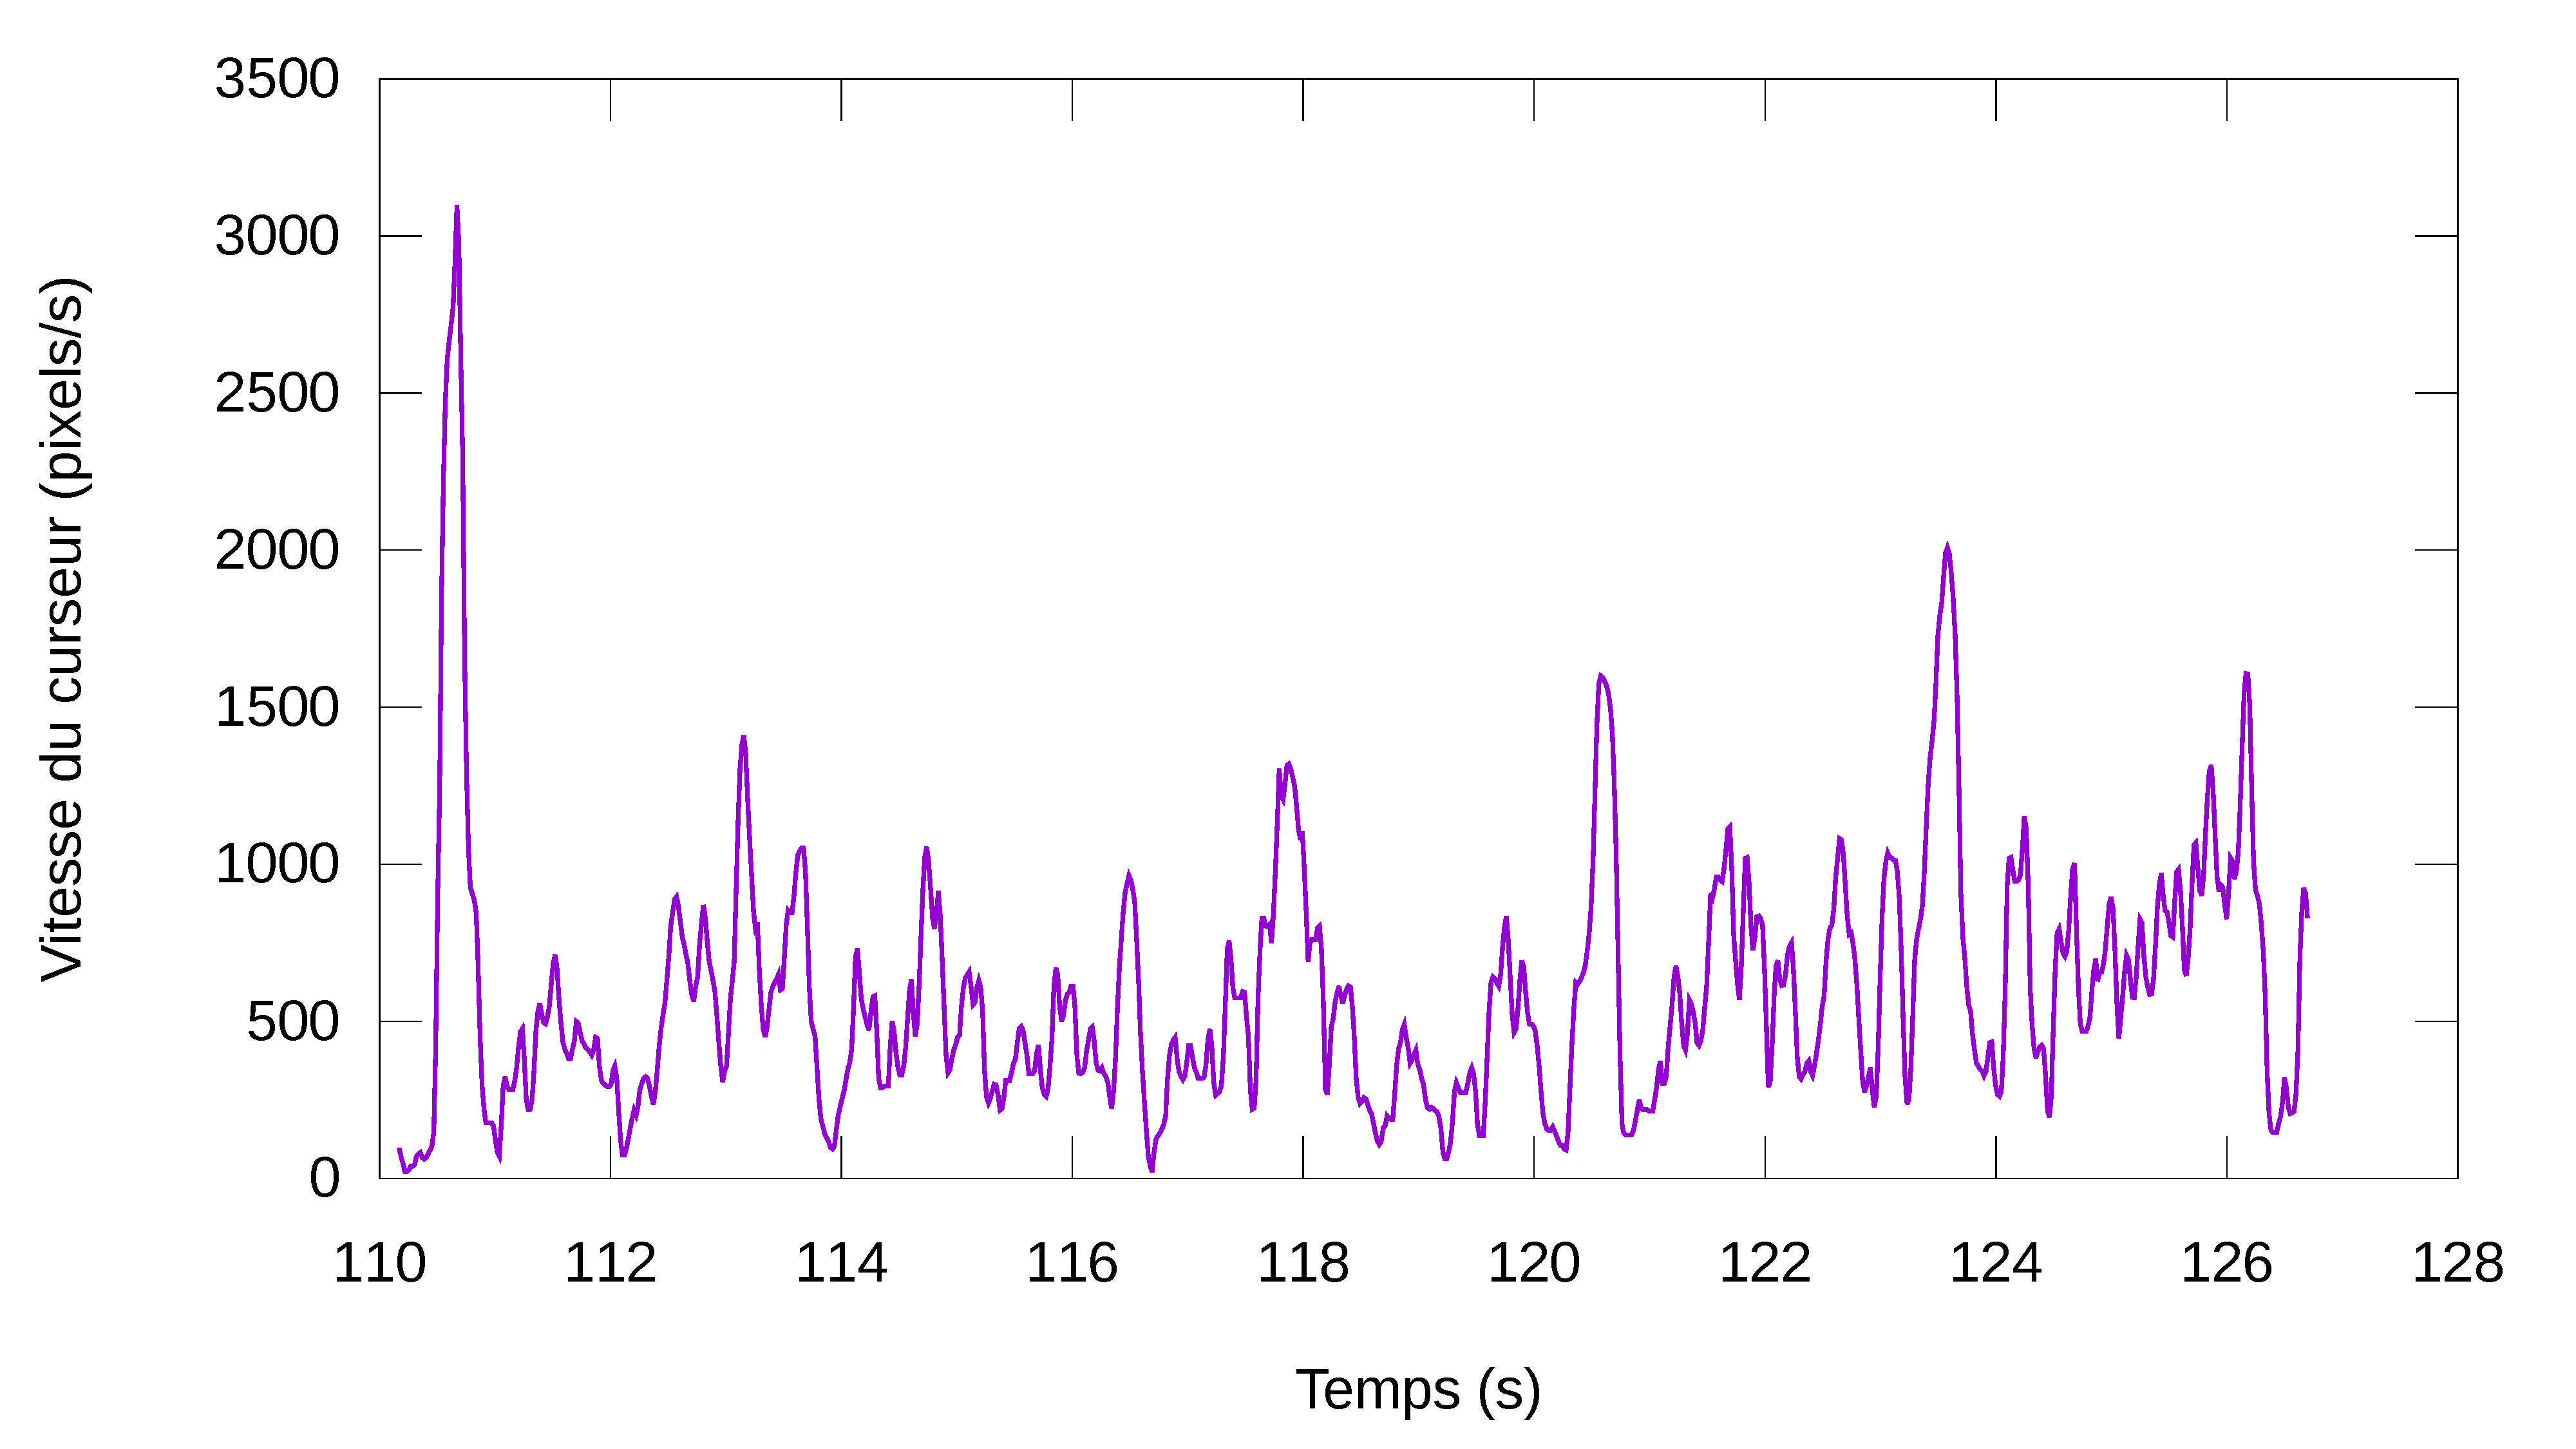
\includegraphics[width=\textwidth]{figures/ch5/profile1}
			\caption{Résultats lissés sur 0,2 seconde.}
			\label{fig:profile1}
		\end{subfigure}
		\caption[Profils de vitesse de curseurs]{Profils de vitesse de curseur, avec et sans lissage.}
		\label{fig:asProfiles}
	\end{figure}
	
	
	\subsection{Interprétation}
	L'objet de cette étude était moins de développer une technique d'aide à la sélection de cibles mobiles que de démontrer la validité et l'utilité de notre modèle d'estimation de la difficulté d sélection d'une cible mobile. En effet, les contraintes placées étaient très fortes, et avaient pour but de tester nos hypothèses \textbf{H1} et \textbf{H2}. Nous retenons la première sans réserves, et la seconde lorsque les performances de sélection sont considérées de manière holistique, et non seulement sur le plan du temps de sélection ou du taux d'erreurs. Une tâche de sélection étant par essence un compromis vitesse-précision, il nous semble que l'hypothèse \textbf{H2} ne devrait pas être rejetée, quoique nous aimerions la voir évaluée plus précisément, avec plus de sujets, voire d'essais par sujet. Ajoutons que les inversions de corrélations notées dans le tableau~\ref{tab:synthRes} plaident pour une légère diminution du paramètre N de la parabole décrite par l'équation~\ref{eq:scalingParabola}, ce qui pourrait également améliorer les résultats.
	
	Cette étude montre qu'il est possible d'estimer de manière relativement fiable la difficulté de sélection d'une cible mobile, et de s'appuyer sur cette donnée pour informer la conception d'une technique d'assistance à la sélection. Notre proposition d'ajustement des tailles des cibles est en effet parfaitement comptabile avec un large éventail de techniques de sélection, parmi lesquelles nous pouvons citer la plupart des curseurs zonaux, comme notamment le \emph{DynaSpot}~\cite{chapuis2009dynaspot}, le lancer de rayon avec désambiguïsation~\cite{grossman2006design}, la sélection en cascade telle que la met en \oe{}uvre le \emph{Disambiguation Canvas}~\cite{debarba2013disambiguation}, par exemple, ou encore l'augmentation des objets, comme avec \emph{Comet}~\cite{hasan2011comet}, par exemple.
	
	\section{Prédiction intentionnelle biaisée -- \emph{SharpHook}}
	Au premier abord, la difficuté de sélection d'une cible pourrait paraître sans intérêt lorsque l'on utilise une heuristique de prédiction intentionnelle telle que \emph{Hook}~\cite{ortega2013hook}, qui ne se préoccuppe pas de la taille des objets. Ce  n'est pas nécessairement vrai.
	
	Certes, la difficulté de sélection d'une cible due à ses mouvements n'a pas d'influence, \emph{a priori}, sur l'intention de l'utilisateur de la sélectionner ou non. Cependant, attendu qu'une heuristique de ce type s'appuie sur un système de scores pour deviner quel objet l'utilisateur cherche à sélectionner, il est possible d'utiliser la difficulté de sélection pour biaiser l'heuristique en faveur des cibles les plus difficiles, de manière tout à fait analogue à ce que nous avons fait avec la taille des cibles dans l'étude précédente. La difficulté pourrait tout simplement, à l'aide d'une parabole du type de celles de la figure~\ref{fig:parabolae}, fournir un facteur permettant de biaiser le score de la cible.
	
	Ainsi, les cibles naturellement faciles seraient certes un peu plus délicates à sélectionner, mais \emph{Hook} est suffisamment performant pour supposer que cela ne pose pas de problème, et les cibles les plus difficiles à saisir seraient plus facilement \og accrochées \fg{} par l'heuristique. Comme nous l'évoquions plus haut, \emph{Hook} est compatible avec les méthodes de filtrages décrites dans la section~\ref{sub:vfaGuide}, et l'ajustement de la taille des cibles peut s'y ajouter sans incompatibilité aucune, quoique sans intérêt manifeste. Notons que ce qui vaut pour \emph{Hook} et son curseur ponctuel vaut également pour \emph{IntenSelect}~\cite{de2005intenselect} et son lancer de rayon avec prédiction intentionnelle.
	
	Nous pouvons formuler deux nouvelles hypothèses :
	
	\begin{description}
		\item[H3 :] Notre estimation de la difficulté de sélection d'une cible est plus fiable que l'usage des paramètres V, F, ou A, même avec une technique de type \emph{Hook}.
		\item[H4 :] Si l'heuristique de prédiction intentionnelle est biaisée en faveur des cibles jugées difficiles, et en défaveur des cibles jugées faciles, les performances de sélection mesurées sur l'ensemble des cibles sont meilleures.
	\end{description}

	
	\subsection{Expérience et protocole}
	Afin d'évaluer ces hypothèses, nous avons mené une étude similaire à celle de la section précédente, avec 8 participants (les mêmes que pour l'étude sur la distance de Fitts). Les mêmes combinaisons de V, F, et A ont été utilisées, mais répétées 20 fois chacune au lieu de 6, pour un total de 520 essais par condition, soit 1040 par passation. Chaque sujet a effectué deux passations, d'où 2080 essais par sujet. Cette multiplication du nombre d'essais fut permise par l'utilisation d'une technique d'aide à la sélection presque identique à \emph{Hook}, avec une différence limitée au retour visuel : au lieu d'un cône (voir la figure~\ref{fig:hookPic}) pointant vers la cible \og accrochée \fg{}, trop instable avec des cibles aussi vives, nous nous sommes contentés de colorer la cible à sélectionner en vert quand elle est accrochée, ce que la figure~\ref{fig:hook_red_green} illustre.
	
	\begin{figure}[!htb]
		\begin{subfigure}[t]{0.49\textwidth}
			\centering
			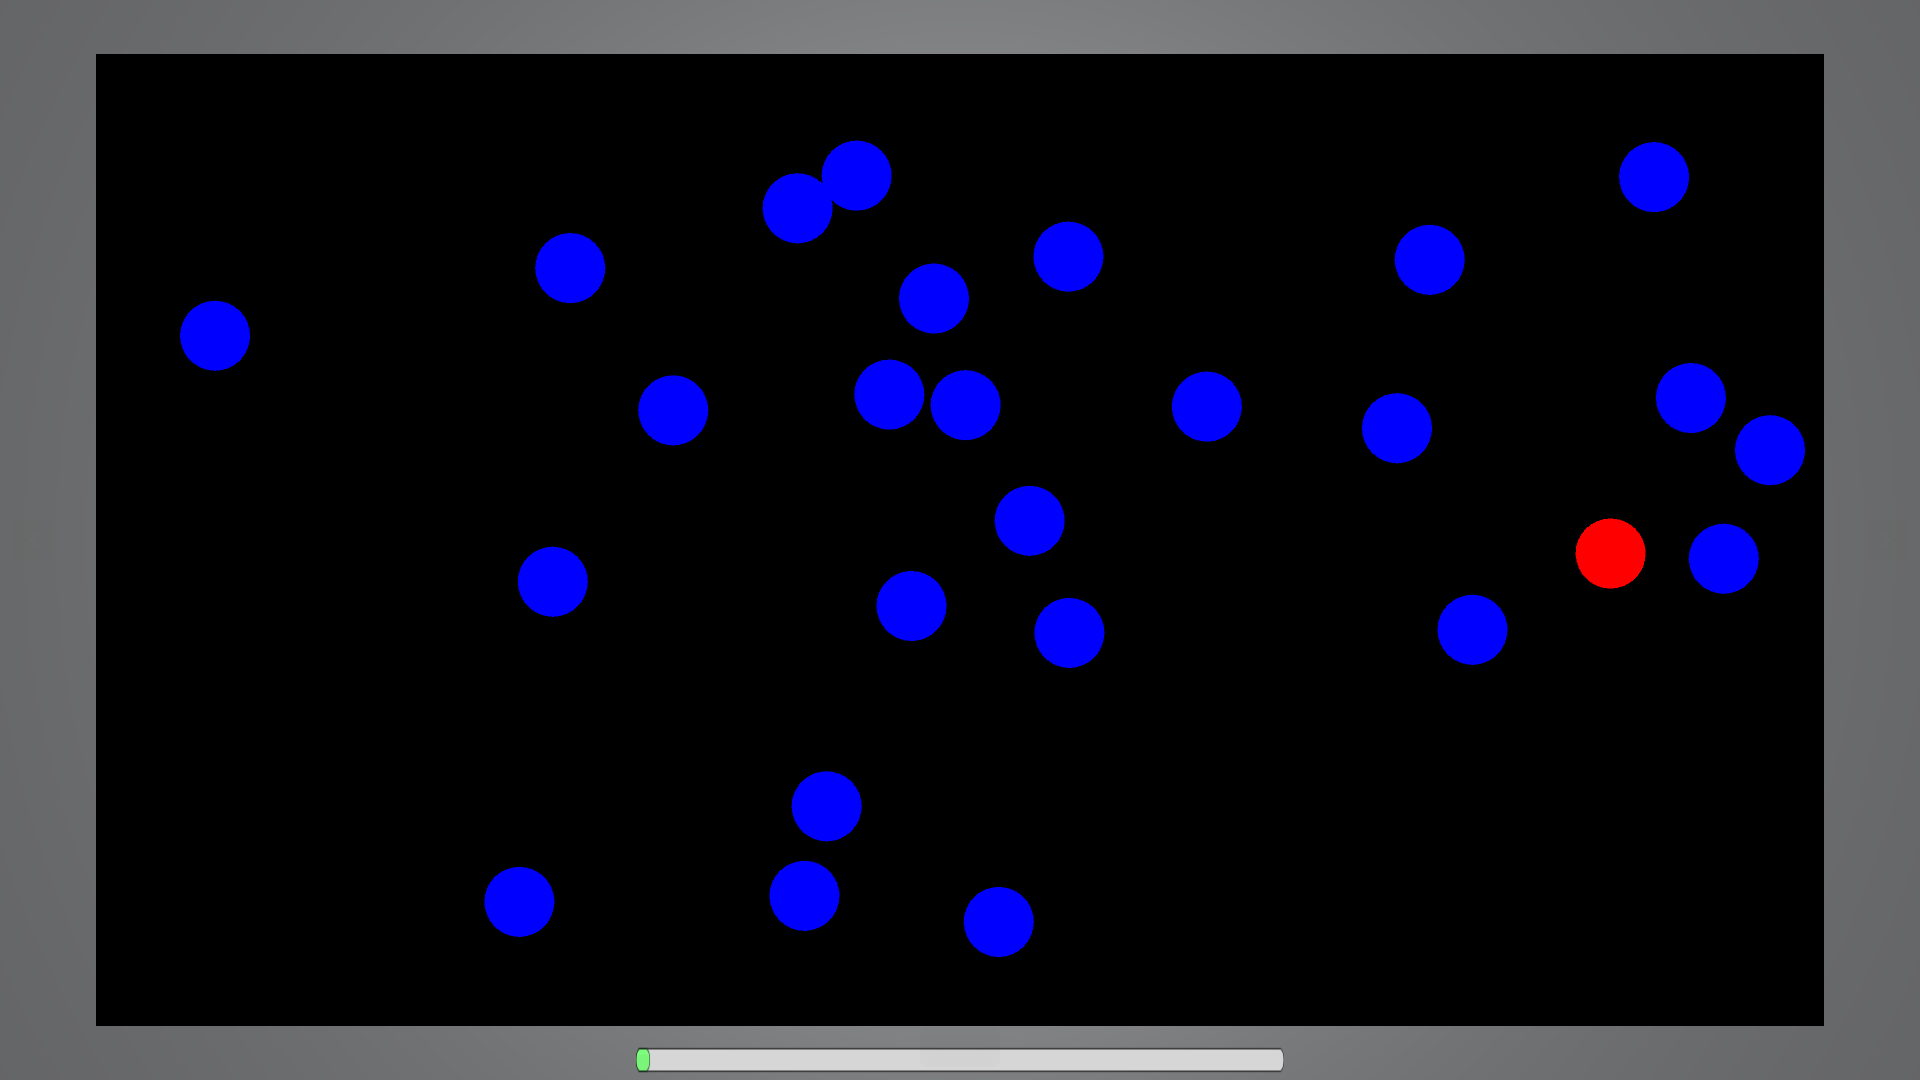
\includegraphics[width=\textwidth]{figures/ch5/hook_red}
			\caption{La cible n'est pas accrochée.}
			\label{fig:hook_red}
		\end{subfigure}
		~
		\begin{subfigure}[t]{0.49\textwidth}
			\centering
			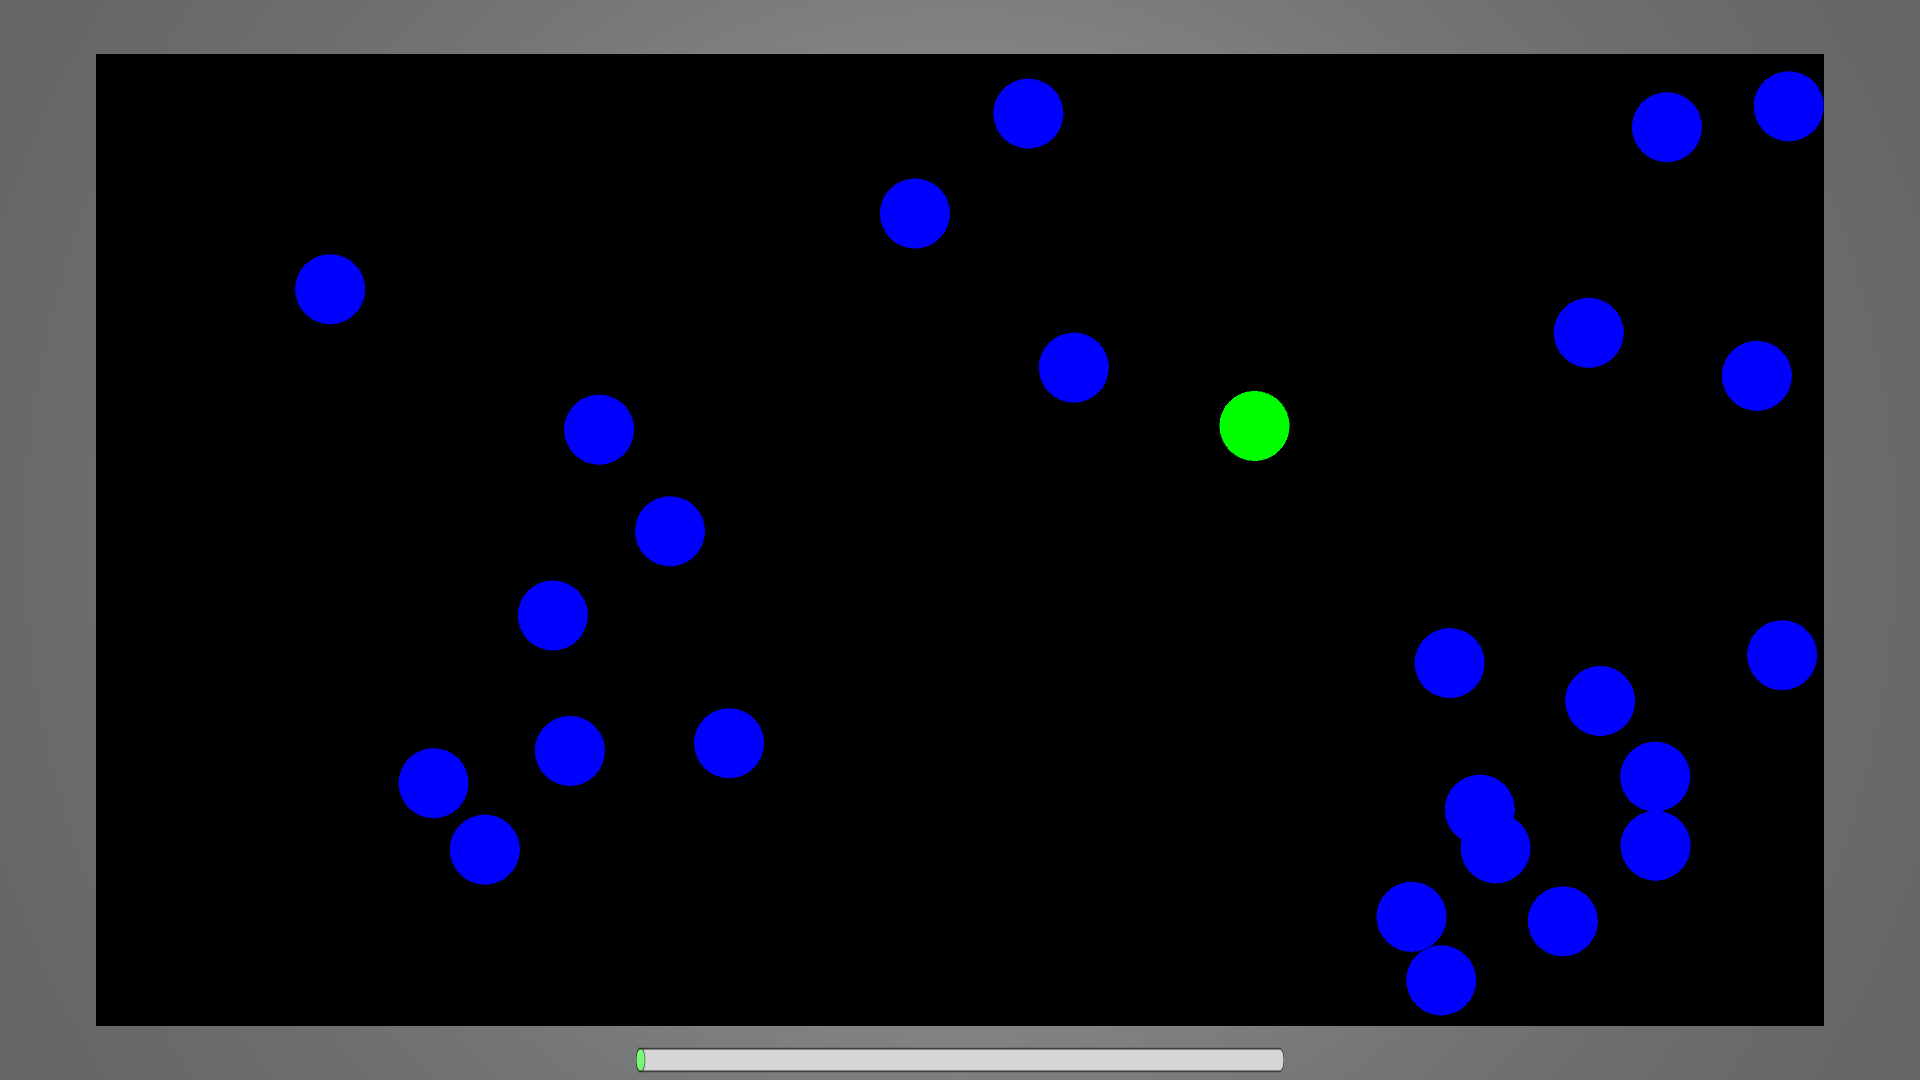
\includegraphics[width=\textwidth]{figures/ch5/hook_green}
			\caption{La cible est accrochée.}
			\label{fig:hook_green}
		\end{subfigure}
		\caption[Application pour l'évaluation de \emph{SharpHook}]{\emph{(Sharp)Hook} : les distracteurs sont bleus, la cible est rouge avant d'être accrochée, puis verte.}
		\label{fig:hook_red_green}
	\end{figure}

	
	\subsection{Score biaisé}
	Pour rappel, l'équation~\ref{eq:standardHookNear} décrit le calcul du score des $NCT$ cibles les plus proches du curseur pour chaque tour de boucle du programme, et l'équation~\ref{eq:standardHookFar} décrit ce calcul des autres cibles, plus distantes. $Score_{cible_{i}}(t)$ est le score de la cible $i$ à l'instant $t$, $NCT$ est le nombre d'objets proches du curseur et $\Delta{}t$ est le temps écoulé depuis la précédente itération. Nous avons ici adopté une valeur de 8 pour NCT, choisie empiriquement.
	
	\begin{align}
		\label{eq:standardHookNear}
		Score_{cible_{i}}(t) &= Score_{cible_{i}}(t-1) + (NCT - i) \times \Delta{}t \\
		\label{eq:standardHookFar}
		Score_{cible_{i}}(t) &= Score_{cible_{i}}(t-1) - \frac{NCT}{2} \times \Delta{}t
	\end{align}
	
	Pour biaiser ce calcul de score, nous avons remplacé ces fonctions par celles des équations~\ref{eq:biasedHookNear} et~\ref{eq:biasedHookFar}. $Diff_{i}$ est une estimation de la difficulté de sélection de la cible $i$, normalisée sur [0,1], où la cible la plus difficile de l'ensemble a une difficulté de 1.

	\begin{align}
		\label{eq:biasedHookNear}
		Score_{cible_{i}}(t) &= Score_{cible_{i}}(t-1) + (NCT - i) \times 2 \times Diff_{i} \times \Delta{}t \\
		\label{eq:biasedHookFar}
		Score_{cible_{i}}(t) &= Score_{cible_{i}}(t-1) - \frac{NCT\times Diff_{i}}{2} \times \Delta{}t
	\end{align}
	
	Bien sûr, ce n'est qu'une façon parmi d'autes de biaiser le calcul du score avec la difficulté de sélection, et d'ailleurs, il serait également possible de biaiser le calcul de la distance. Nous proposons cette solution avant tout pour sa simplicité. Celle-ci étant dérivée de \emph{Hook}, mais se voulant plus astucieuse, nous l'avons baptisée \emph{SharpHook}.
	
	\subsection{Temps de sélection et erreurs}
	Les résultats bruts obtenus avec \emph{SharpHook} sont présentés sur la figure~\ref{fig:rawHookPerfs}, où la condition \og Standard \fg{} correspond à la prédiction intentionnelle fondée sur l'heuristique de \emph{Hook}, et la condition \emph{Biaisé} correspond à \emph{SharpHook} et son score biaisé en fonction de la difficulté de sélection de chaque cible. Les temps de sélection présentés sur la figure~\ref{fig:hookRawTimes} montre un léger avantage en faveur de \emph{SharpHook}, mais avec des intervalles de confiance à 95~\%{} se chevauchant : [1,7373 ; 1,9736] pour \emph{Hook} et [1,6080 ; 1,8159] pour \emph{SharpHook}. Toutefois, l'avantage de ce dernier est beaucoup plus marqué pour les taux d'erreurs, présentés sur la figure~\ref{fig:hookRawErrors}. De fait, nous retenons l'hypothèse \textbf{H4}. Des vues plus synthétiques des performances sont présentées sur la figure~\ref{fig:hookRawProducts}, qui représente le produit $Temps(Erreurs+1)$, et la figure~\ref{fig:rawHookErrorsTimesScatter}, qui représente les performances de sélection sur deux axes : temps et erreurs.
	
	\begin{figure}[!htb]
		\begin{subfigure}[t]{0.49\textwidth}
			\centering
			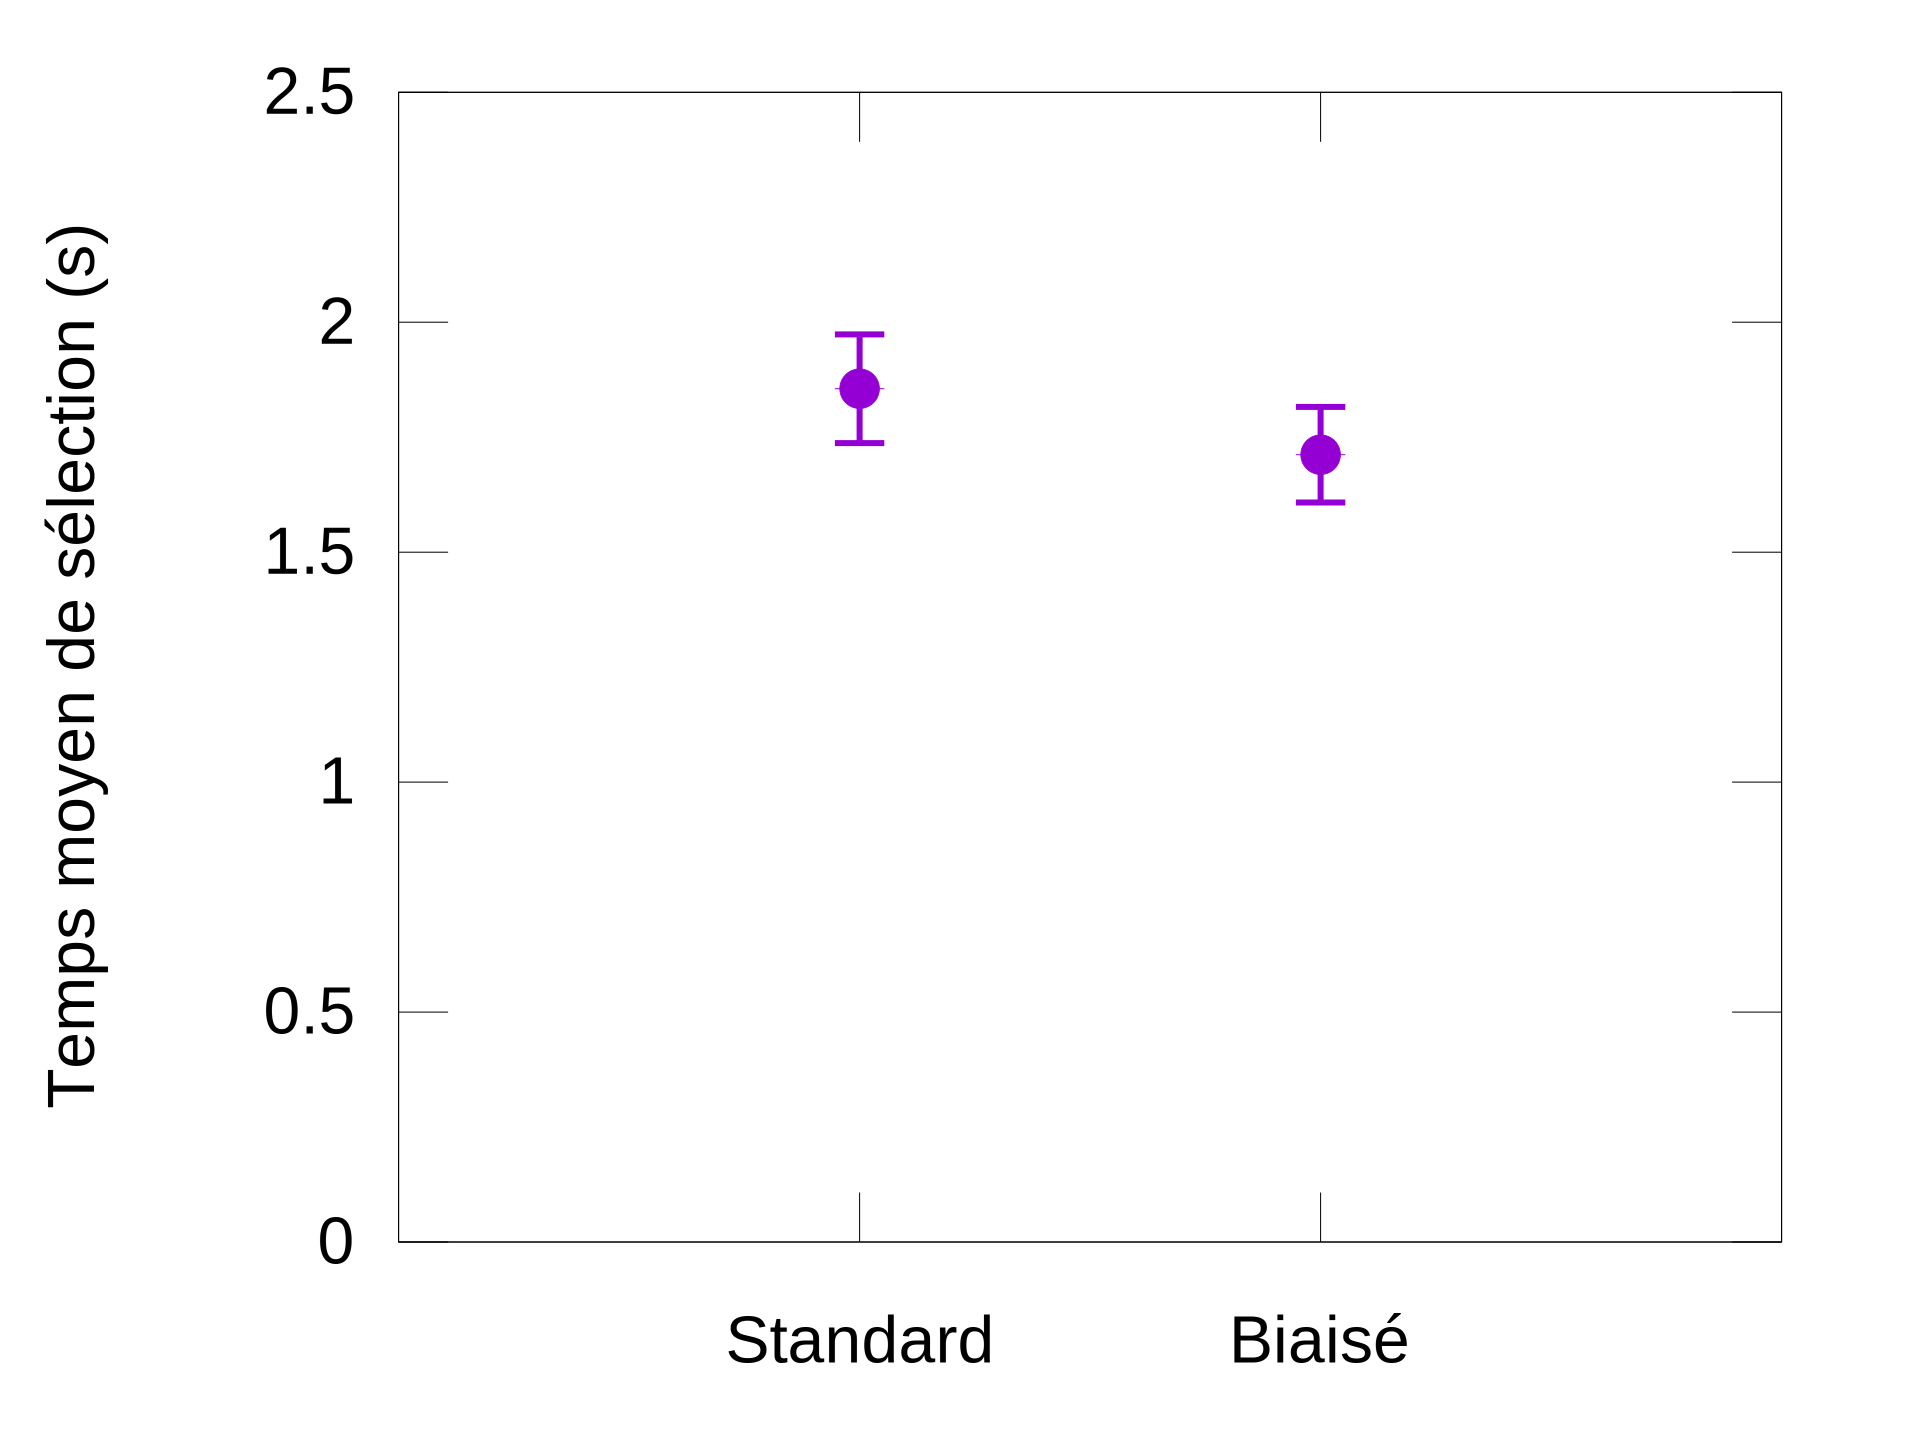
\includegraphics[width=\textwidth]{figures/ch5/hookRawTimes}
			\caption{Temps de sélection bruts.}
			\label{fig:hookRawTimes}
		\end{subfigure}
		~
		\begin{subfigure}[t]{0.49\textwidth}
			\centering
			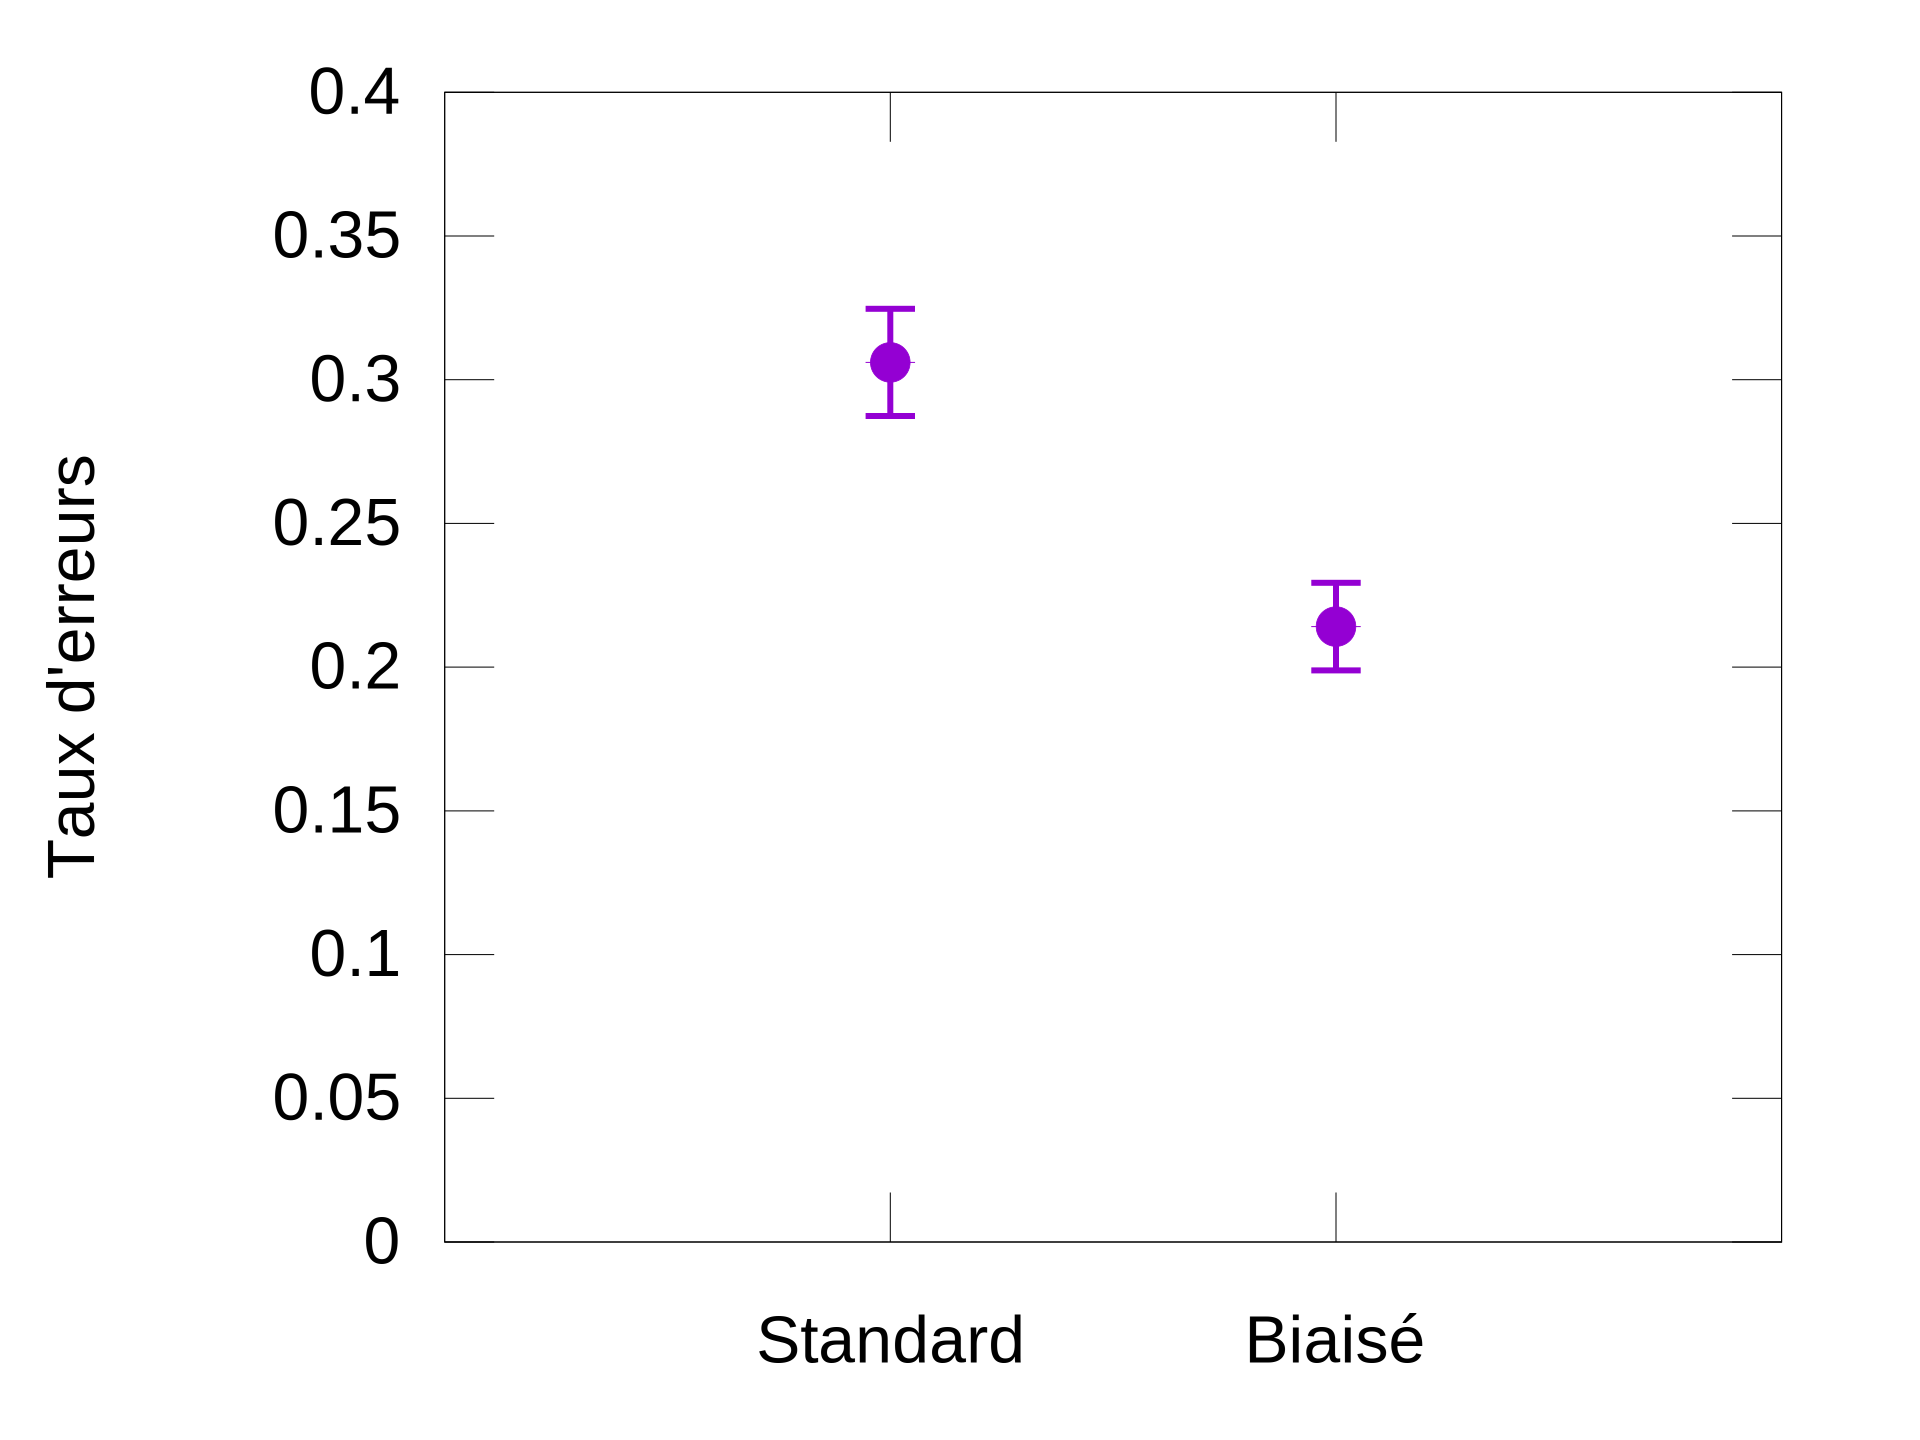
\includegraphics[width=\textwidth]{figures/ch5/hookRawErrors}
			\caption{Nombres moyens d'erreurs bruts.}
			\label{fig:hookRawErrors}
		\end{subfigure}
		~
		\begin{subfigure}[t]{0.49\textwidth}
			\centering
			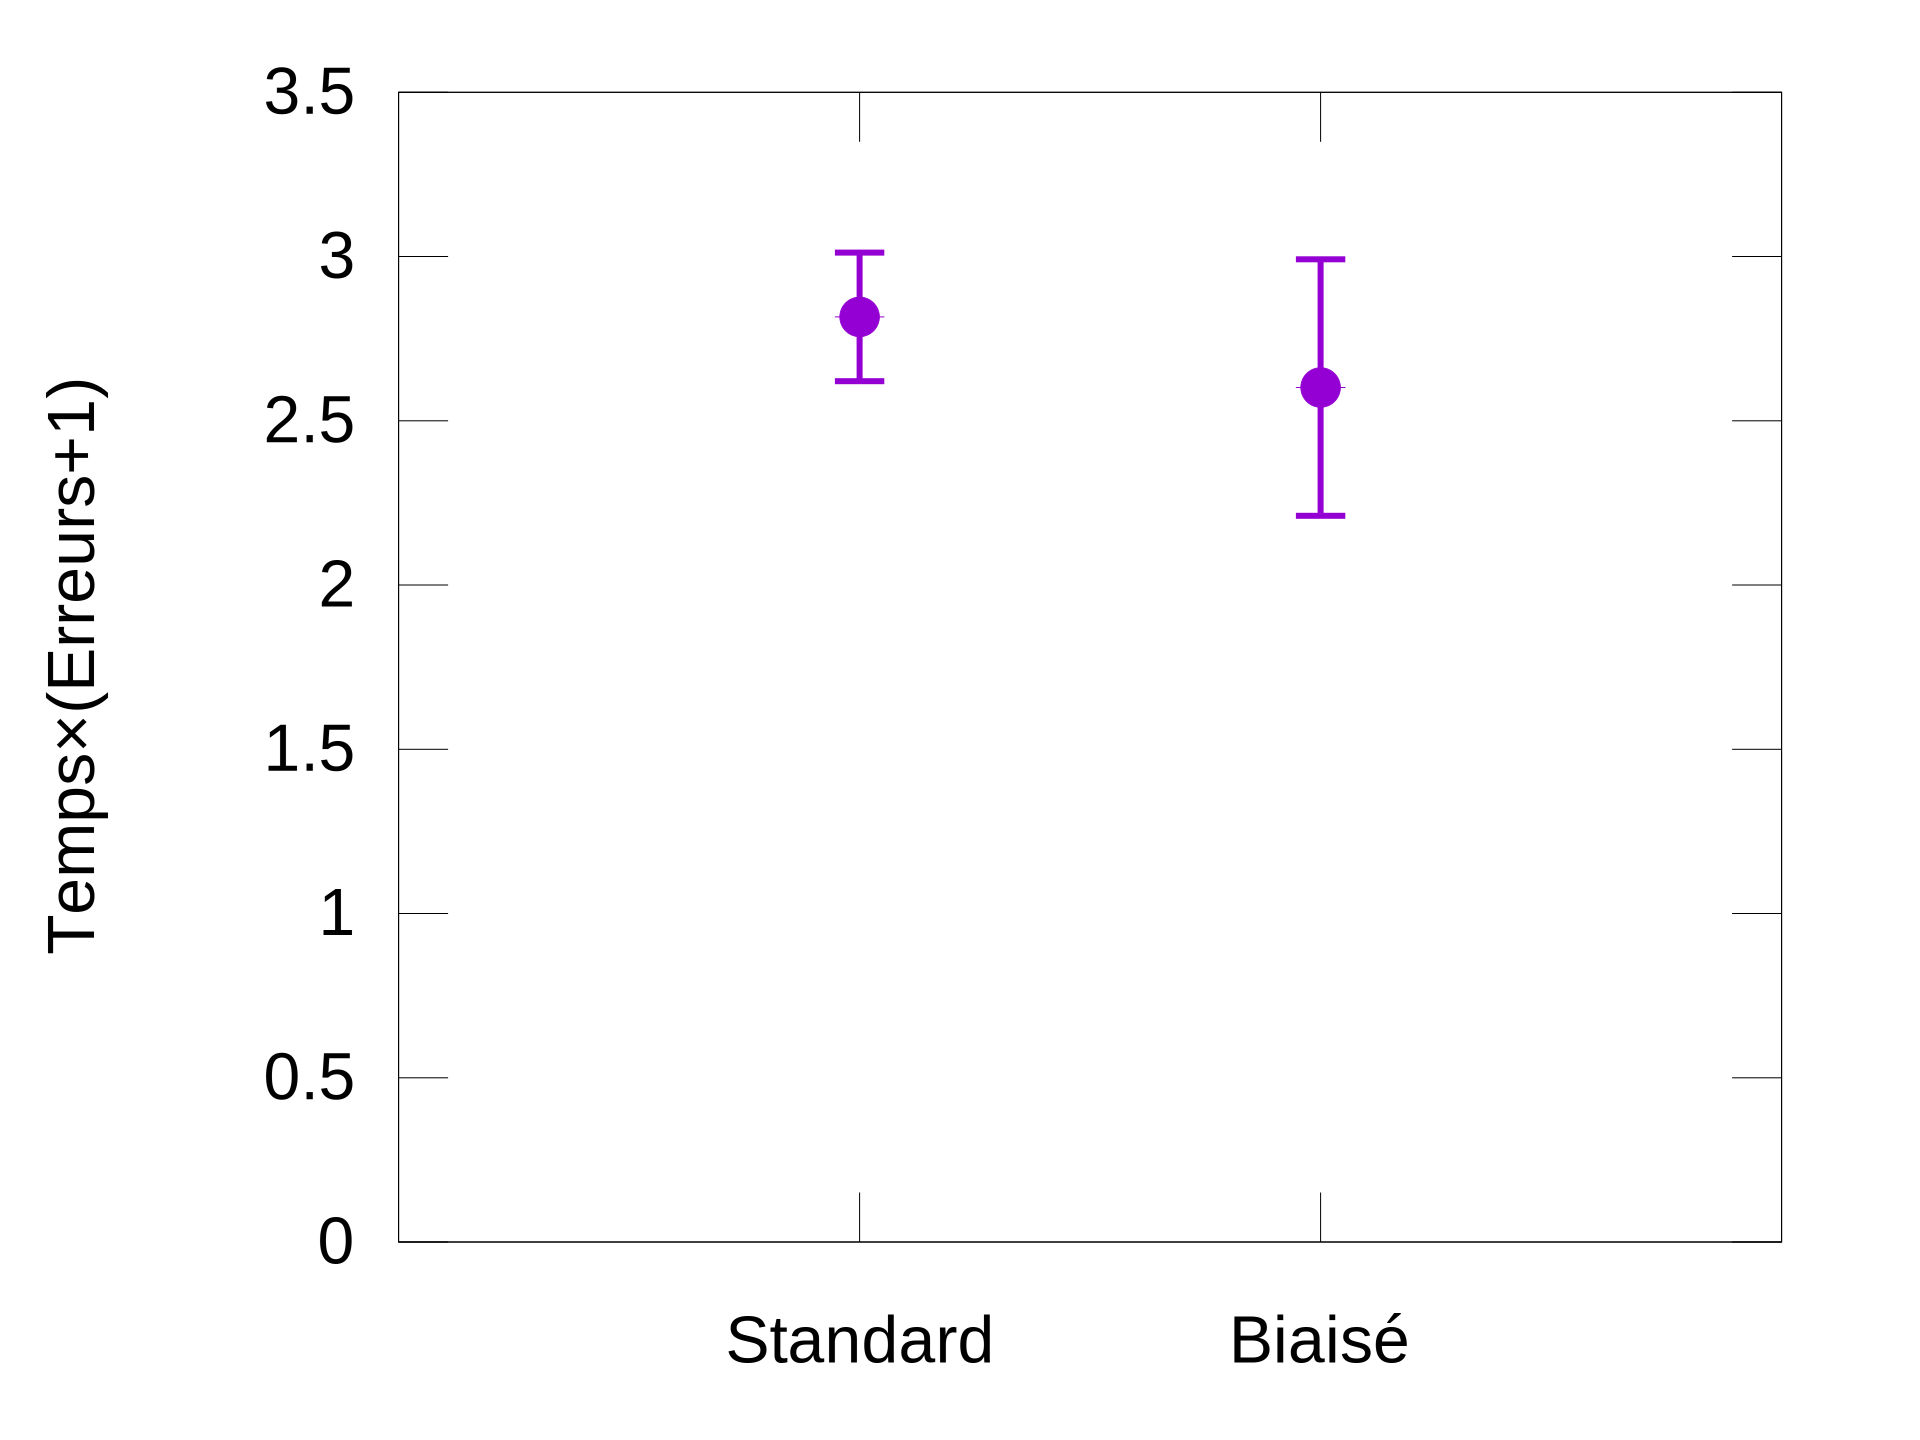
\includegraphics[width=\textwidth]{figures/ch5/hookRawProducts}
			\caption{Produits $T(E+1)$ bruts.}
			\label{fig:hookRawProducts}
		\end{subfigure}
		~
		\begin{subfigure}[t]{0.49\textwidth}
			\centering
			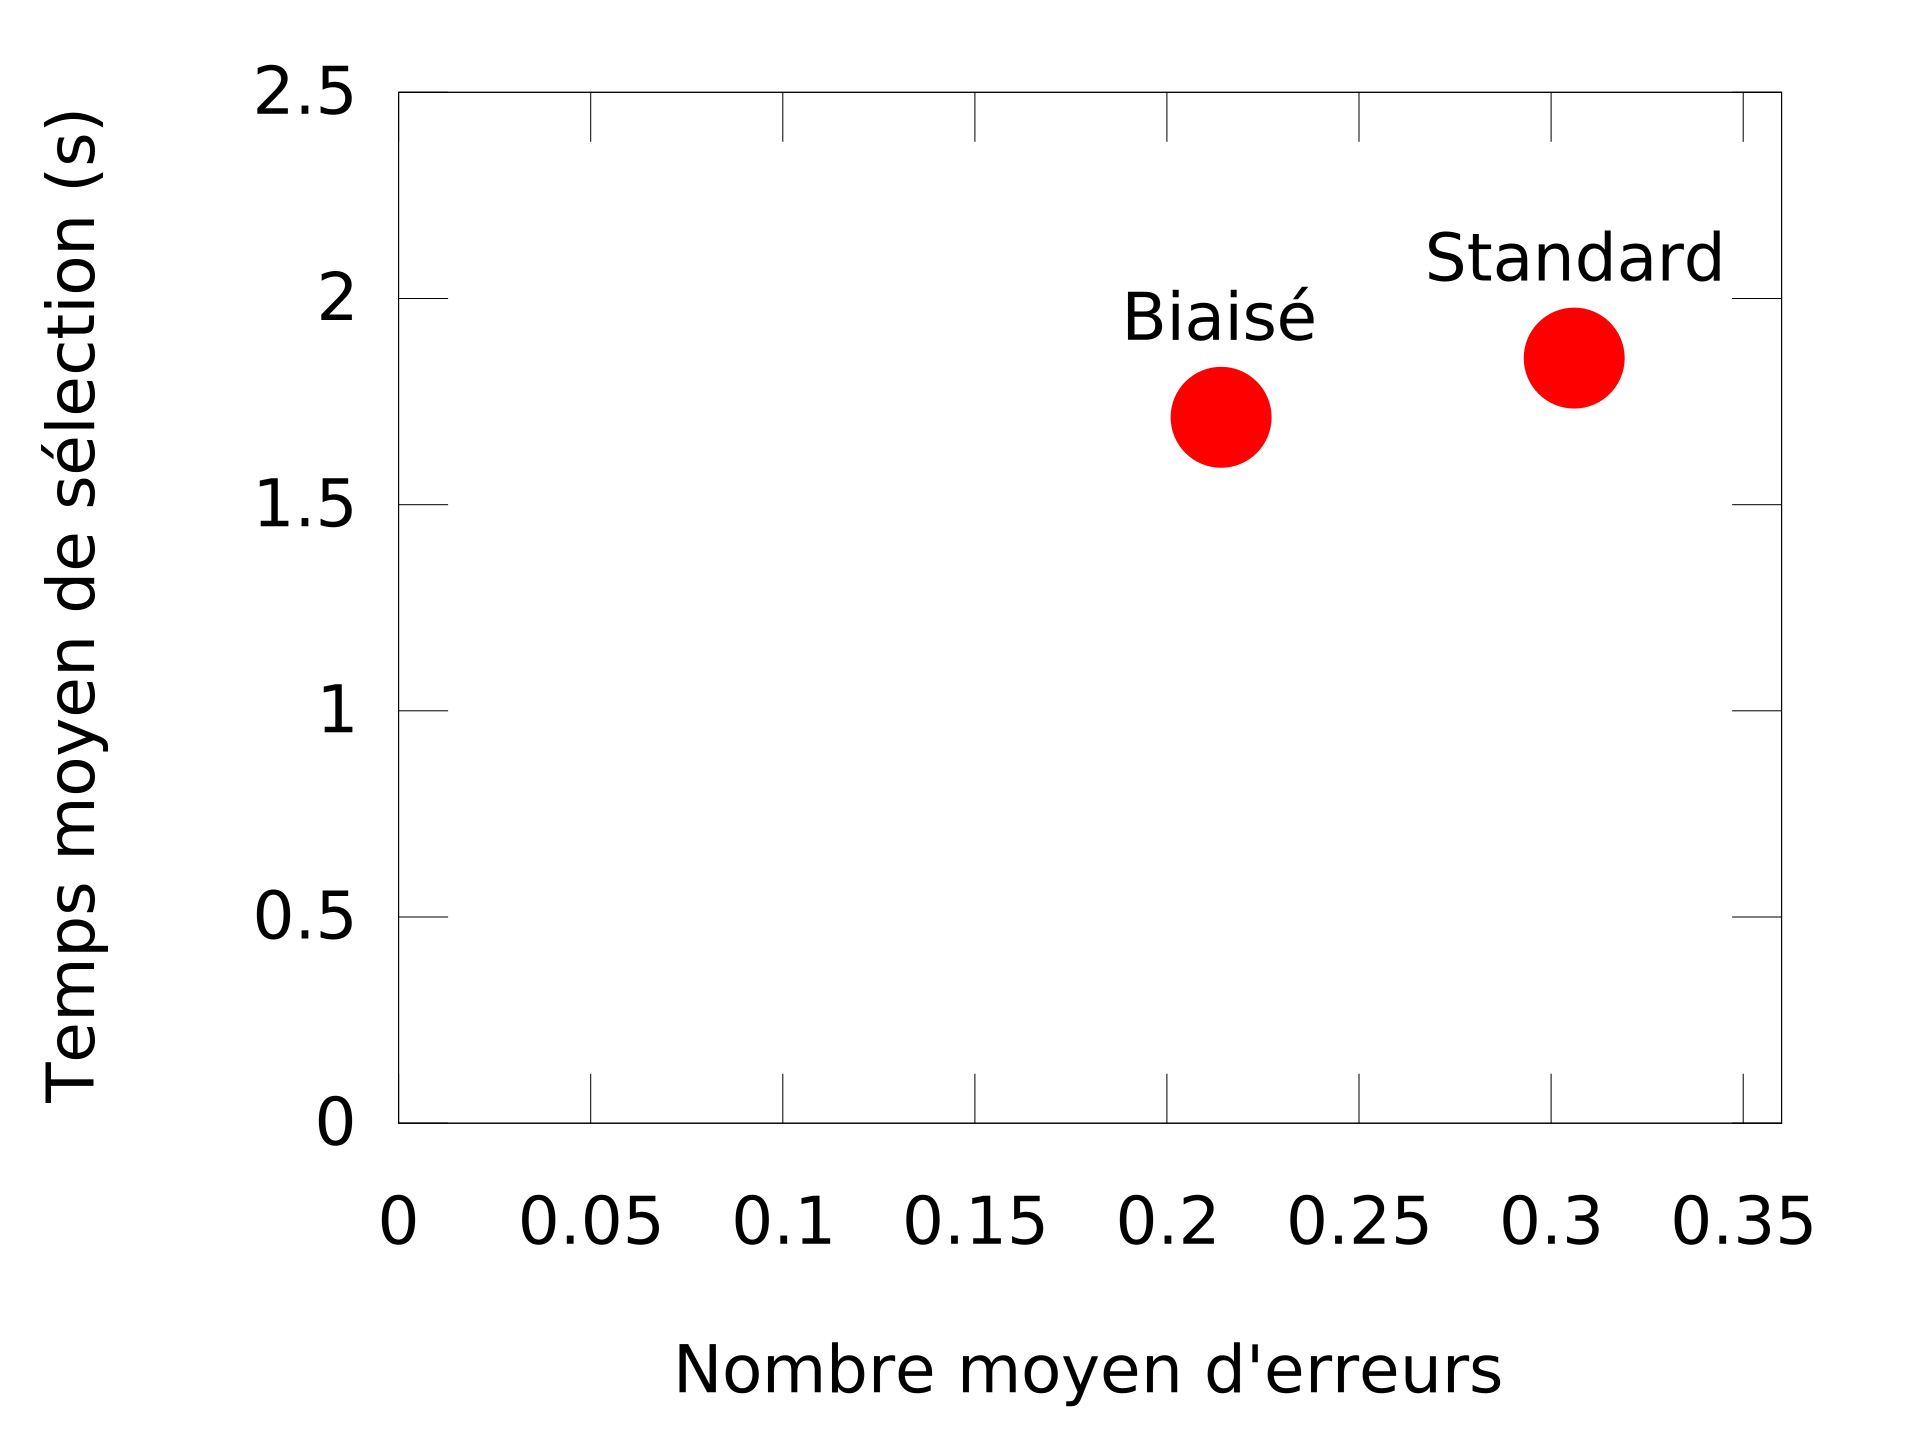
\includegraphics[width=\textwidth]{figures/ch5/rawHookErrorsTimesScatter}
			\caption{Temps de sélection et erreurs.}
			\label{fig:rawHookErrorsTimesScatter}
		\end{subfigure}
		\caption[\emph{SharpHook} -- résultats bruts]{Performances de sélection de \emph{SharpHook} -- résultats bruts. Moyennes et intervalles de confiance à 95~\%{}.}
		\label{fig:rawHookPerfs}
	\end{figure}
	
	\subsection{Normalisation des résultats}
	Ici aussi, et pour les mêmes raisons que précédemment, nous avons normalisés nos mesures. Les résultats sont présentés sur la figure~\ref{fig:normHookPerfs}. Dans celle-ci, MTSN est la moyenne des temps de sélection normalisés, et MTEN est la moyenne des taux d'erreurs normalisés. Cette fois-ci, les valeurs moyennes sont représentées par les barres horizontales sombres, tandis que les extrémités des \og boîtes \fg{} indiquent les bornes des intervalles de confiance à 95~\%{}, et les \og moustaches \fg{} indiquent les bornes des intervalles de confiance à 99~\%{}. Pour une meilleure lisibilité, les échelles ne commencent pas à zéro.
	
	Sur la base de résultats normalisés, les données sont plus clairement en faveur de \emph{SharpHook}. Celui-ci conserve son avantage tant en temps de sélection qu'en taux d'erreurs, mais les intervalles de confiance sont clairement disjoints, même à 99~\%{}. Notre hypothèse \textbf{H4} s'en trouve confortée.


	\begin{figure}[!htb]
		\begin{subfigure}[t]{0.49\textwidth}
			\centering
			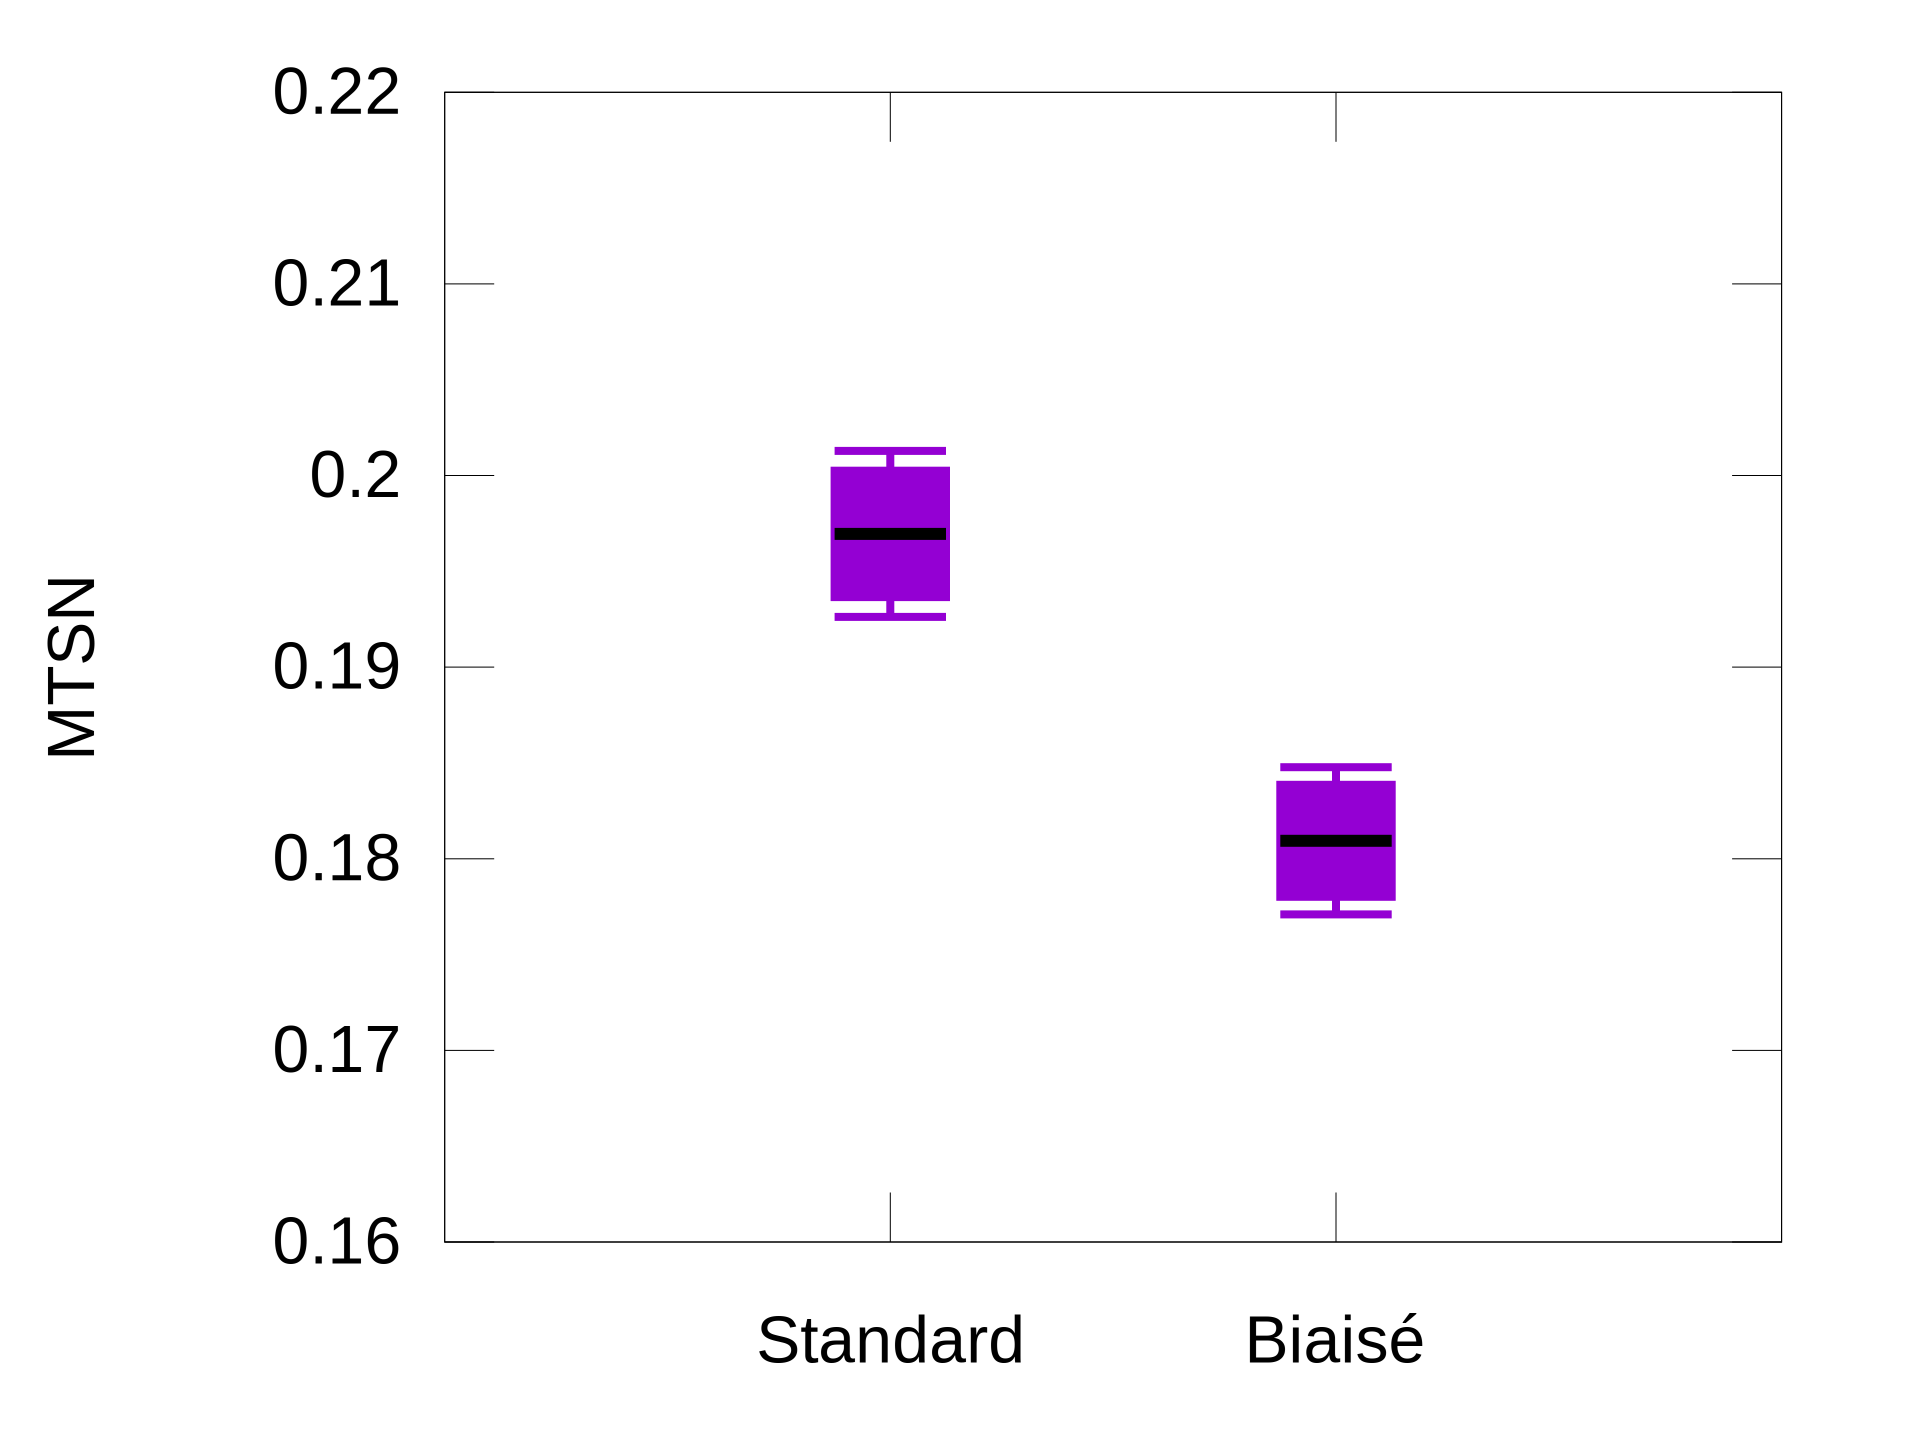
\includegraphics[width=\textwidth]{figures/ch5/hookNormTimes}
			\caption{MTSN.}
			\label{fig:hookNormTimes}
		\end{subfigure}
		~
		\begin{subfigure}[t]{0.49\textwidth}
			\centering
			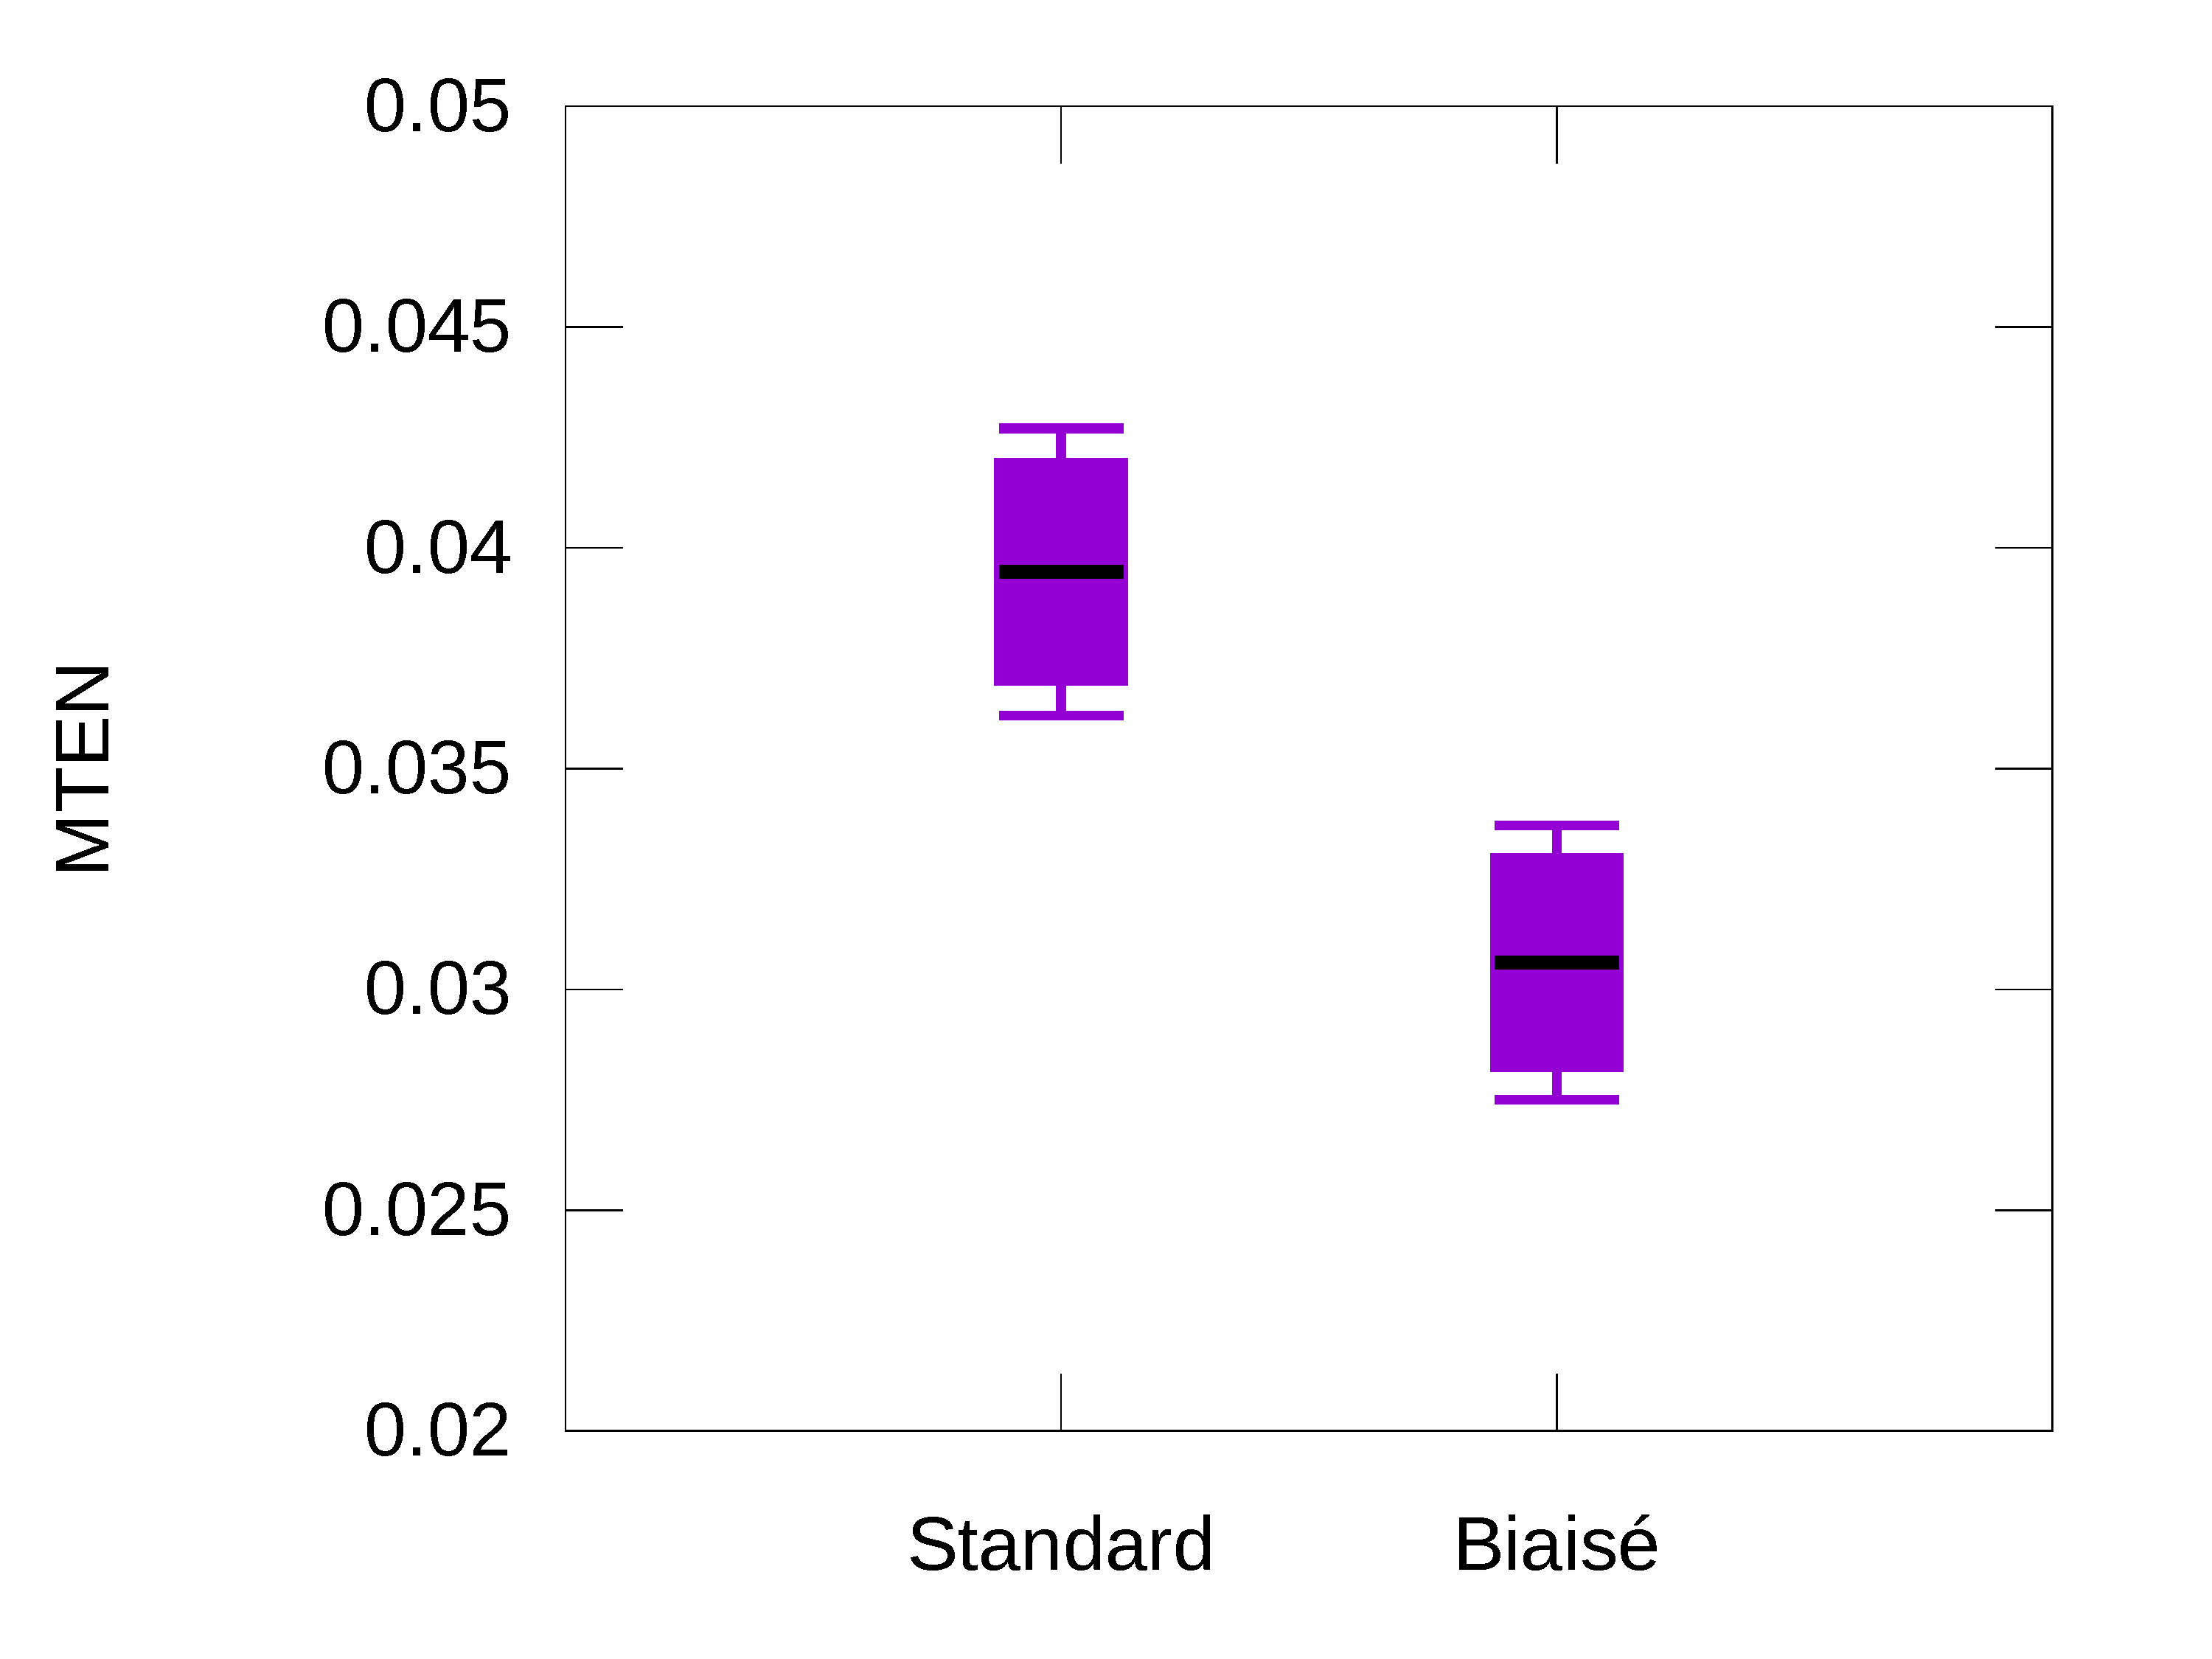
\includegraphics[width=\textwidth]{figures/ch5/hookNormErrors}
			\caption{MTEN.}
			\label{fig:hookNormErrors}
		\end{subfigure}
		~
		\begin{subfigure}[t]{0.49\textwidth}
			\centering
			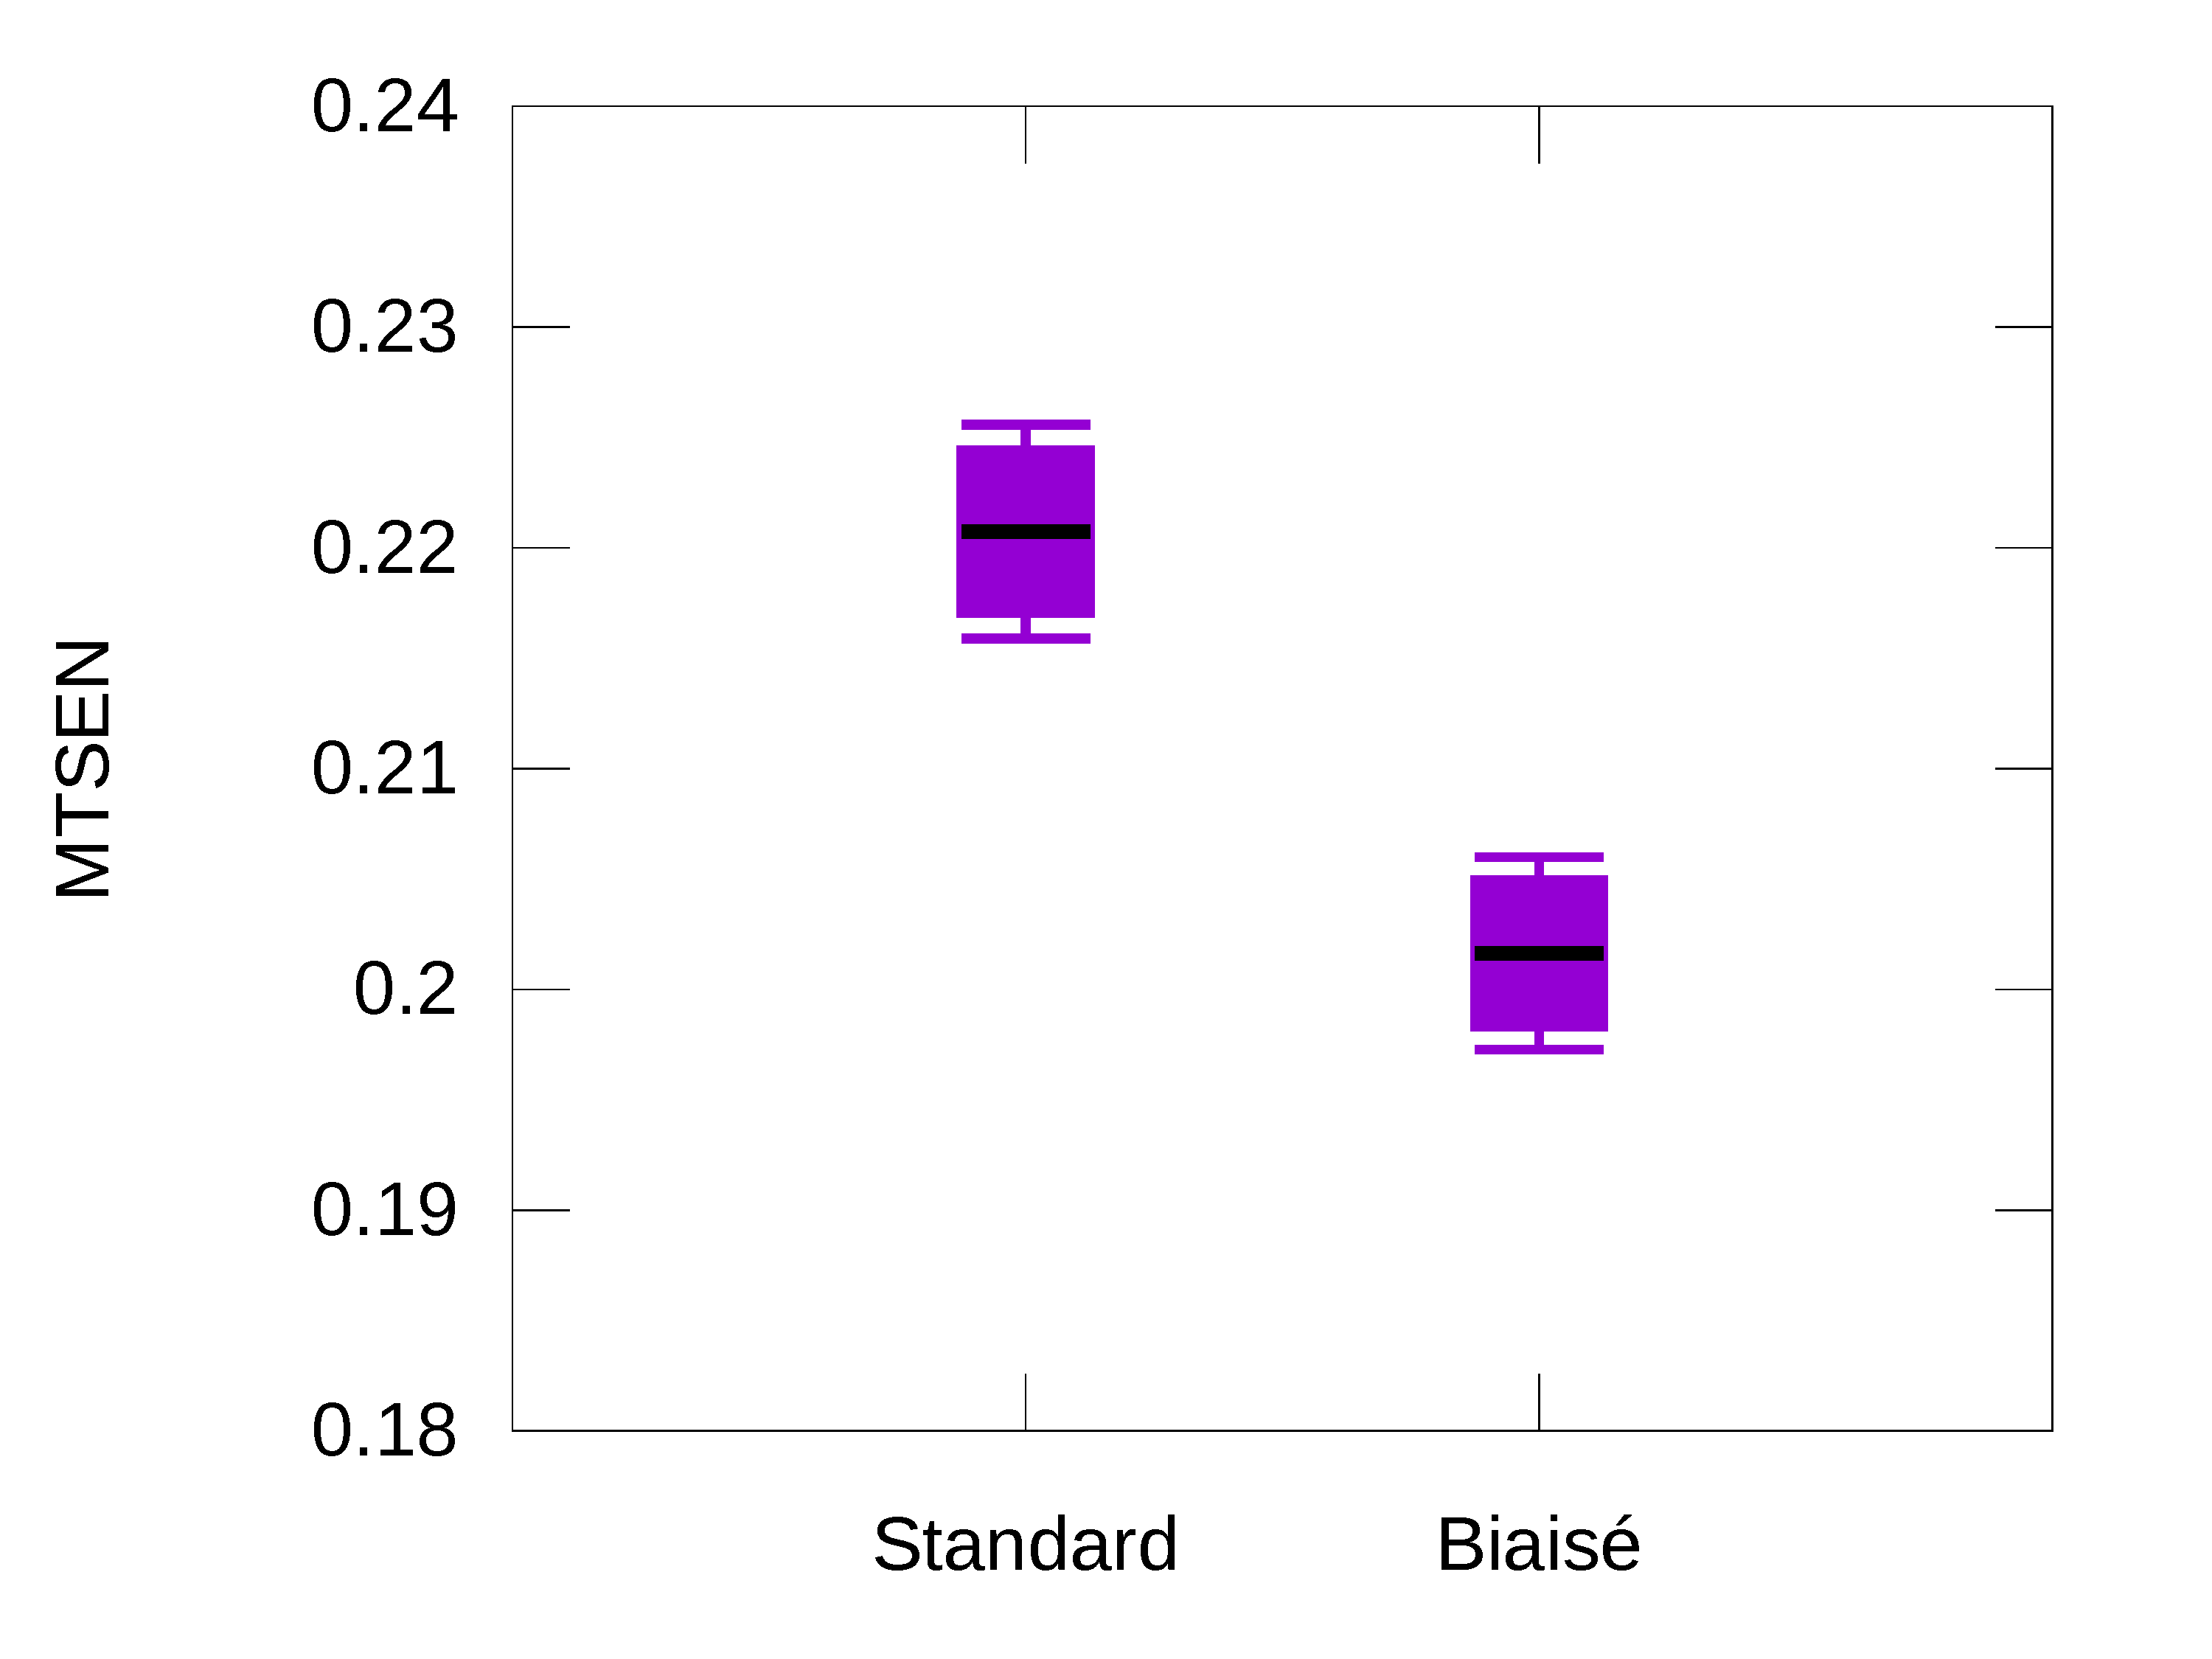
\includegraphics[width=\textwidth]{figures/ch5/hookNormProducts}
			\caption{Moyennes des performances sur E et T normalisés.}
			\label{fig:hookNormProducts}
		\end{subfigure}
		~
		\begin{subfigure}[t]{0.49\textwidth}
			\centering
			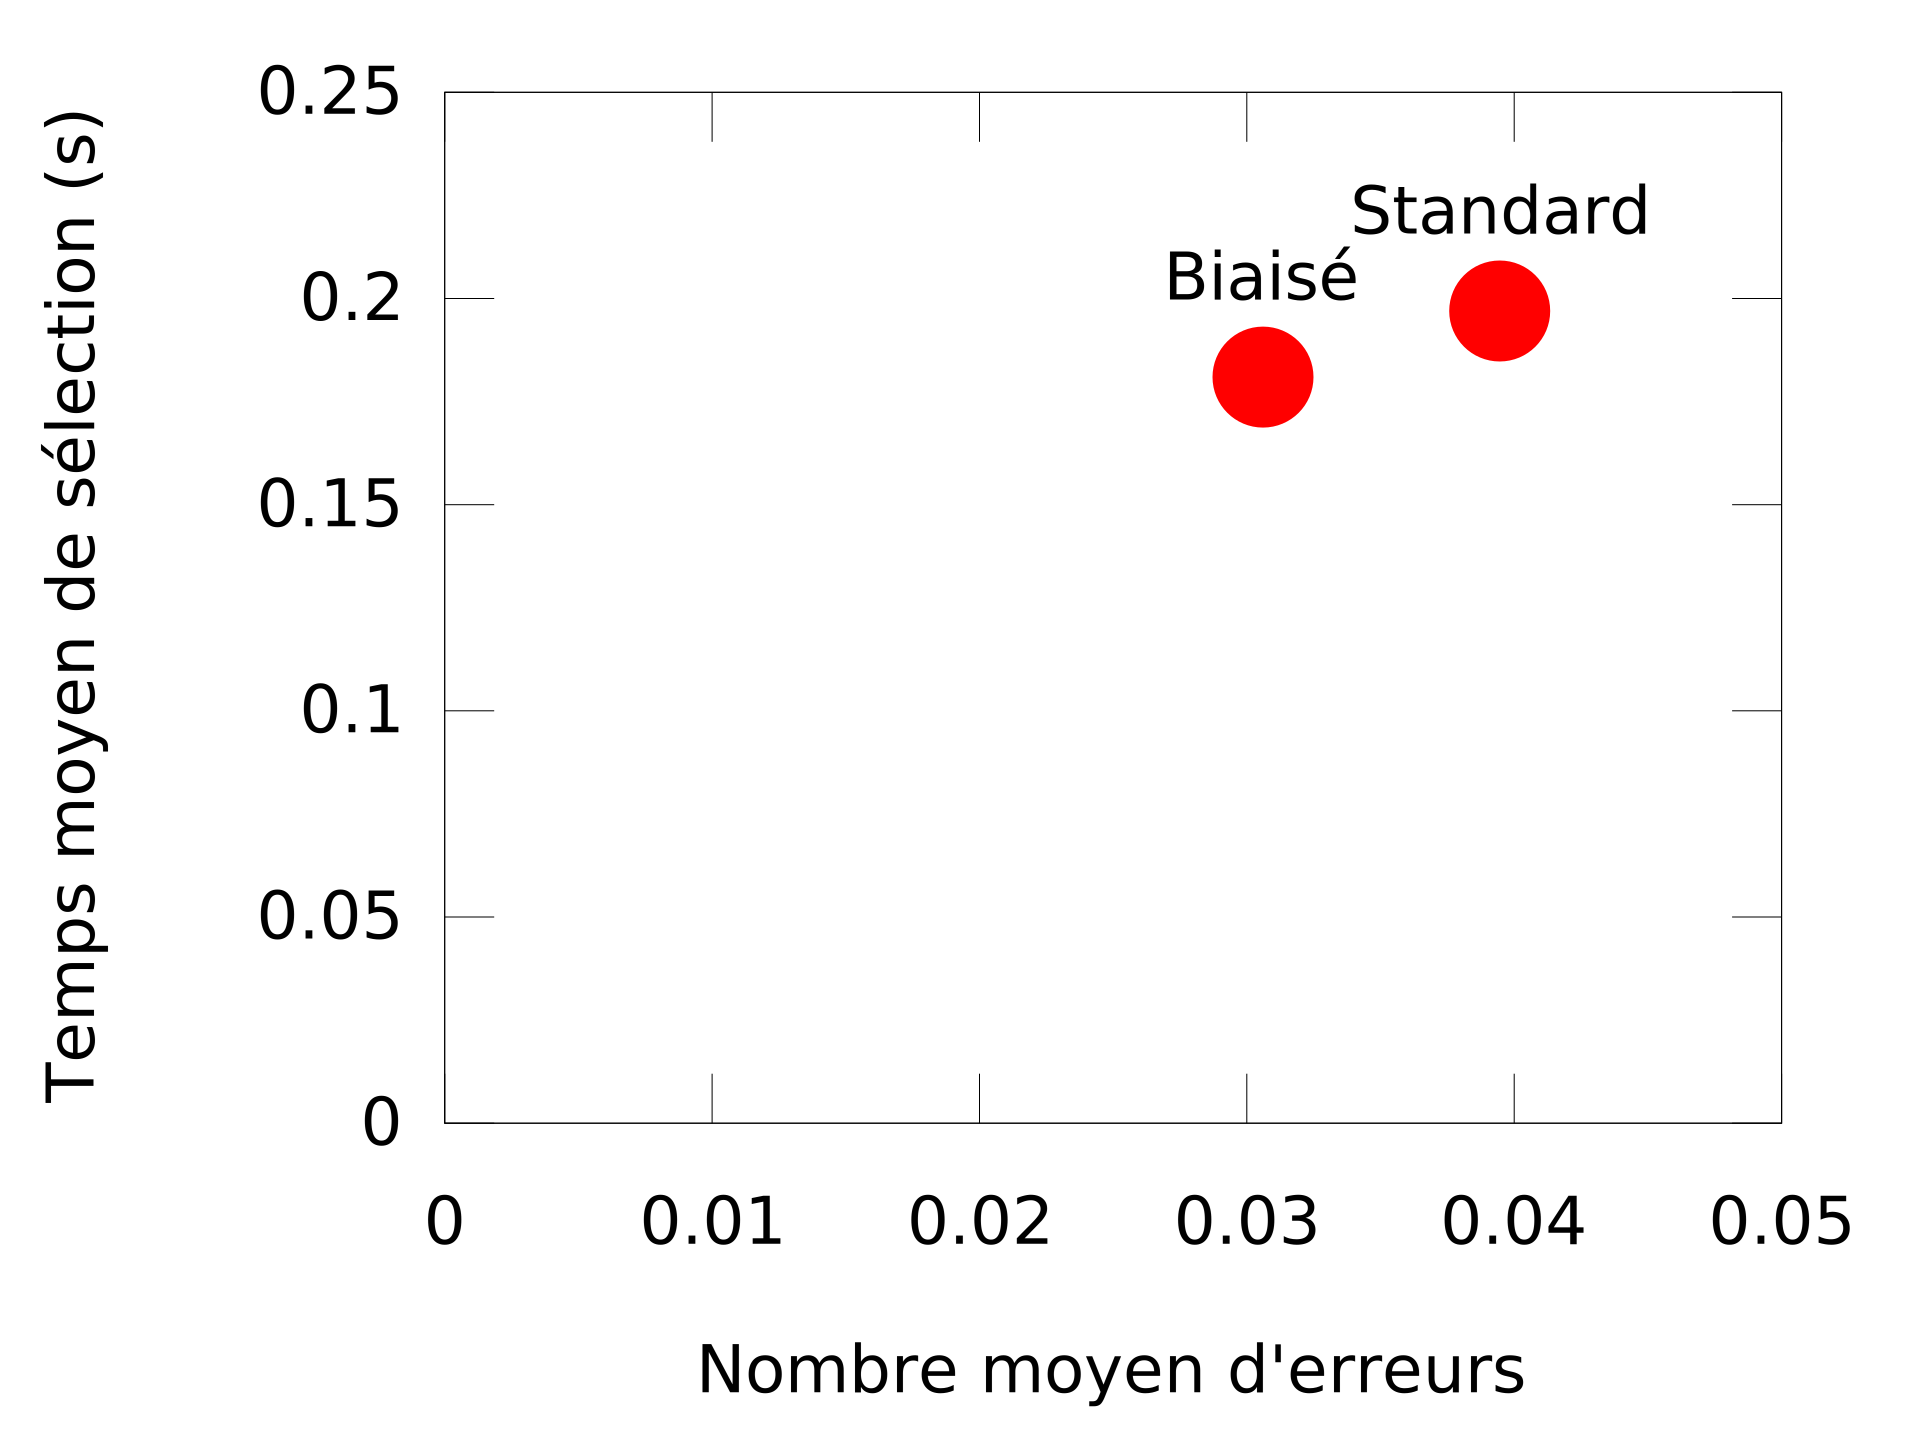
\includegraphics[width=\textwidth]{figures/ch5/normHookErrorsTimesScatter}
			\caption{MTSN et MTEN.}
			\label{fig:normHookErrorsTimesScatter}
		\end{subfigure}
		\caption[\emph{SharpHook} -- résultats normalisés]{Performances de sélection de \emph{SharpHook} -- résultats normalisés. Moyennes, intervalles de confiance à 95~\%{} et à 99~\%{}.}
		\label{fig:normHookPerfs}
	\end{figure}
	
	\subsection{Difficulté et performances}
	Sur les résultats normalisés, d'intéressantes corrélations sont observables, et présentées dans le tableau~\ref{tab:hookCorr}. En effet, s'il n'y a pas de corrélation significative entre VFA et les erreurs (ces dernières étant sans doute trop rares), il y a bien des corrélations marquées, quoique faibles, entre V et les temps de sélection. Surtout, notre estimation de la difficulté est plus fortement corrélée aux temps de sélection que la vitesse. Il est surtout intéressant de remarquer que même \emph{SharpHook} présente une corrélation entre la difficulté et les temps de sélection, ce qui suggère que le biais que nous avons introduit dans le calcul du score pourrait être plus bénéfique s'il était renforcé, par exemple en élevant le facteur $Diff$ au carré, ou en biaisant également le calcul de la distance.
	
	\begin{table}
		\centering
		\begin{tabular}{l | c c c c}
			Condition			& \emph{Hook}				& \emph{SharpHook}			& \emph{Hook} (n)			& \emph{SharpHook} (n)	\bigstrut[b] \\ \hline
			C($d$, $T$)			& 4,92 ; 7,0$.10^{-6}$		& 3,26 ; 3,0$.10^{-16}$		& 11,90 ; 1,3$.10^{-27}$	& 8,86 ; 5,7$.10^{-16}$	\bigstrut[t] \\
			C($V$, $T$)			& 3,09 ; 4,8$.10^{-3}$		& 3,92 ; 3,5$.10^{-4}$		& 8,92 ; 3,6$.10^{-16}$		& 7,65 ; 2,9$.10^{-12}$	\\
		\end{tabular}
		\caption[\emph{Hook} et \emph{SharpHook} -- corrélations]{Corrélations (exprimées en pourcentages) entre $V$ ou l'estimation de la difficulté $d$ d'une part, et les temps de sélection d'autre part. La mention \og (n) \fg{} indique les résultats normalisés.}
		\label{tab:hookCorr}
	\end{table}

	Ces corrélations sont bien moins marquées que sans assistance à la sélection. Il est probable que cette assistance lisse les écarts de performance d'une condition à l'autre, réduisant de fait les corrélations qui en découlent. Quoi qu'il en soit, la \emph{p-value} associée à la corrélation entre la difficulté et le temps de sélection étant inférieure à celle de la corrélation entre V et le temps de sélection, et ce de plus de 10 ordres de grandeur, nous pouvons retenir notre hypothèse \textbf{H3}.
	
	
	\subsection{Interprétation}
	Nos résultats illustrent l'intérêt de l'utilisation du modèle VFA et d'une estimation de la difficulté de sélection s'appuyant dessus pour biaiser une heuristique de prédiction intentionnelle. Cependant, ils mettent également en lumière le fait que ce biais peut s'appliquer de bien des façons, et qu'un calibrage minutieux pourrait s'avérer bénéfique. En effet, nous n'avons pas entièrement \og annulé \fg{} la corrélation entre la difficulté et les performances de sélection avec la version de \emph{SharpHook} que nous proposons.
	
	De plus, il n'est pas garanti que le modèle d'estimation de la difficulté de sélection que nous proposons, et qui s'appuie sur des données relatives à des sélection non assitées, soit optimal pour \emph{Hook}, qui change profondément la nature de la tâche. Il pourrait donc être opportun de concevoir un modèle spécifique, permettant un biais pus précis et donc plus performant. Enfin, nos résulats confirment ceux d'Ortega~\cite{ortega2013hook}, d'une part en montrant que les temps de sélection avec \emph{Hook} sont très courts --- nos résultats étant indirectement comparables à ceux de la section~\ref{sub:as_res}, obtenus avec d'autres sujets et un autre dispositif expérimental --- mais surtout, les taux d'erreurs sont exceptionnellement bas : autour de 0,25 par sélection contre environ 9,5 sans assistance.
	
	\section{Assistance haptique ou pseudo-haptique -- \emph{FastHook}}
	Ces taux d'erreurs découlent avant tout de stratégies \og imprudentes \fg{} de la part de participants ayant prévilégié la vitesse au détriment de la précision, mais ils reflètent une réelle difficulté lors de l'utilisation de \emph{Hook}, et par conséquent de \emph{SharpHook} : lorsqu'une cible est accrochée, l'utilisateur peut la sélectionner, mais il n'a pas de garantie qu'entre sa décision de cliquer pour effectuer la sélection, et le clic effectif, la cible sera toujours accrochée. Et parfois, elle se décroche, l'heuristique ayant changé de prédiction entre-temps.
	
	En fait, il est possible de favoriser la \og sûreté \fg{} d'une sélection, en suivant une cible plus longtemps et/ou de plus près, afin que son score soit très supérieur à ceux des autres objets, pour réduire la probabilité que le score d'un autre objet dépasse celui de la cible visée entre la décision de cliquer et le clic. Cette stratégie échange de la vitesse contre de la précision. Or, comme nous l'avons vu dans le chapitre~\ref{chap1}, pour certaines applications, cette dernière est primordiale.
	
	Nous avons plusieurs fois mentionné l'intérêt potentiel d'une assistance haptique ou pseudo-haptique~\cite{lecuyer2009simulating, pusch2011pseudo} lors d'une tâche de sélection. Dans ce contexte précis au moins, elle pourrait présenter deux intérêts : réduire la probabilité d'une erreur en attirant le curseur vers la cible accrochée, donc en réduisant la distance entre les deux et en améliorant le score de la cible ; accrocher la cible de plus près, permettant de creuser plus rapidement l'écart de score avec les autres objets, et donc de sélectionner plus rapidement. En principe, un avantage pourrait être observé, ou l'autre, ou un peu des deux.
	
	\subsection{Déplacement du curseur}
	Pour évaluer l'intérêt de ce concept, nous avons développé une nouvelle variante de \emph{Hook}, augmentée d'une assistance pseudo-haptique attirant le curseur vers la cible prédite par l'heuristique. À chaque tour de boucle du programme, le curseur subit le déplacement effectif $\vec{dep_{eff}}$ décrit par les équations~\ref{eq:phDisplacement} et~\ref{eq:phDisplacement2}, où $K$ est une constante réelle ; $V$ est la vitesse de la cible accrochée ; $f_{accrochage}$ est le score de la cible accrochée divisé par le score le plus élevé relevé sur l'ensemble des autres objets ; $\vec{cc}$ est un vecteur de norme 1 ayant pour origine le curseur, et orienté vers la cible ; $\Delta{}t$ est le temps écoulé depuis la précédente boucle ; et $distance$ est la distance entre le curseur et la cible.

	\begin{align}
		\label{eq:phDisplacement}
		\vec{dep_{eff}} &= max(\vec{dep}, \vec{cc}) \\
		\label{eq:phDisplacement2}
		\vec{dep} &= \frac{K * V * f_{accrochage} * \vec{cc} * \Delta{}t}{1 + distance^{2}}
	\end{align}
	
	Cette variante de \emph{Hook} permettant d'accrocher plus fermement une cible, nous l'appelons \emph{FastHook}\footnote{Par opposition à \emph{loose} plus qu'à \emph{slow}.}. Nous formulons à son propos les hypothèses suivantes :
	
	\begin{description}
		\item[H5 :] Notre estimation de la difficulté de sélection d'une cible est plus fiable que l'usage des paramètres F ou A, même avec une technique de type \emph{FastHook}.
		\item[H6 :] Grâce à son assistance pseudo-haptique, \emph{FastHook} offre de meilleures performances que \emph{Hook} :
		\begin{description}
			\item[H6a :] Les temps de sélection de \emph{FastHook} sont meilleurs que ceux de \emph{Hook}.
			\item[H6b :] Les taux d'erreurs de \emph{FastHook} sont meilleurs que ceux de \emph{Hook}.
		\end{description}
	\end{description}
	
	\subsection{Décrochage manuel}
	Bien que l'assistance pseudo-haptique puisse être utile, elle a parfois l'inconvénient de \og bloquer \fg{} l'utilisateur sur un distracteur. Il peut en effet arriver que le curseur passe trop de temps près d'un distracteur et que celui-ci voie son score grimper de telle sorte que la force d'accrochage ($f_{accrochage}$) devienne très grande. Il est alors extrêmement difficile de se dégager de ce distracteur pour accrocher la bonne cible. Afin de permettre aux utilisateurs d'éviter ce problème, nous avons ajouté une fonction de \og décrochage \fg{} manuel : via un clic sur le bouton secondaire de la souris, les scores de toutes les cibles sont remis à zéro. Notons cependant qu'il serait peut-être préférable de ne remettre à zéro que le score de l'objet actuellement accroché. Par souci d'équité, nous avons également ajouté cette fonction à la version de base de \emph{Hook}, attendu que l'accrochage d'un distracteur peut aussi être nuisible sans assistance pseudo-haptique, quoique dans une moindre mesure.
	
	\subsection{Assistance à double tranchant}
	Plus généralement, et les retours de nos participants vont tous dans ce sens, l'assistance pseudo-haptique a l'inconvénient, tant que la bonne cible n'est pas accrochée, d'attirer le curseur vers un distracteur. Nous avons tâché de pondérer le calcul du déplacement du curseur de façon à limiter cet inconvénient, mais il demeure présent et, parfois, gênant, même avec la possibilité de décrocher manuellement. En retour, lorsque la bonne cible est accrochée, le curseur est attirée vers elle et elle risque moins d'être décrochée. De fait, l'assistance est contre-productive avant l'accrochage, et potentiellement utile après, surtout si l'on cherche à s'assurer de la sûreté de l'accrochage avant d'effectuer la sélection. La stratégie de sélection peut donc avoir une influence sur l'effet de l'assistance pseudo-haptique.
	
	C'est la raison pour laquelle nous avons 

	
	\subsection{Expérience et protocole}
	Même avec la version standard de \emph{Hook}, nous l'avons vu, les erreurs sont assez rares. Pour mesurer l'influence de \emph{FastHook} sur celles-ci, nous avons décidé de favoriser leur occurrence, en choisissant des paramères VFA extrêmement difficiles, en conjonction avec un grand nombre de distracteurs :
	
	\begin{description}
		\item[V :] 16 largeurs de cadre par seconde, soit 45,44~cm/s (1 valeur)
		\item[F :] 8 ; 12 ; 16 ; 20 ; 24 ; 28 ; 32 ; 36 ; 40 ; 44 ; 48 ; 52 ; 56 ; 60~Hz (14 valeurs)
		\item[A :] 30 ; 60 ; 90 ; 120 ; 150 ; 180\textdegree{} (6 valeurs)
	\end{description}
	
	Nous avons donc $1\times{}14\times{}6 = 84$ combinaisons différentes, auxquelles s'ajoute une combinaison rectiligne. Chaque combinaison était évaluée deux fois par sujet, pour un total de $(84+1)\times{}2 = 170$ essais par sujet. Le grand nombre de combinaisons est lié à la nécessité d'un grand nombre de distracteurs pour augmenter la difficulté de la tâche, nous permettant une grande diversité dans les natures de leurs mouvement. À cette vitesse, les cibles traversent la largeur de l'écran en une seconde seulement, de sorte que même en mouvement rectiligne, elles sont difficiles à saisir. Sans assistance à la sélection, cette expérience serait probablement impossible.
	
	L'expérience menée était par ailleurs identique à celle portant sur \emph{SharpHook}, avec les mêmes sujets, et des cibles de taille réduite, afin de limiter l'encombrement visuel : de 18,5~mm de diamètre, elles passent à 11,4~mm. De plus, deux sessions d'entraînement précédaient les passations : une sans assistance pseudo-haptique, et une avec. Cela nous parut nécessaire compte tenu de la difficulté de prise en main de l'assistance pseudo-haptique --- nous y reviendrons plus bas. La figure~\ref{fig:pseudohaptics} fournit une illustration de l'environnement d'évaluation. Cette image ne permet toutefois pas de se représenter la difficulté extrême des sélections à réaliser, aussi invitons-nous le lecteur à se référer à un enregistrement vidéo que nous avons mis en ligne\footnote{\url{https://www.youtube.com/watch?v=hv9IYbEzR3s} -- la vitesse de lecture de la vidéo est réglable.}.
	
	\begin{figure}[!htb]
		\centering
		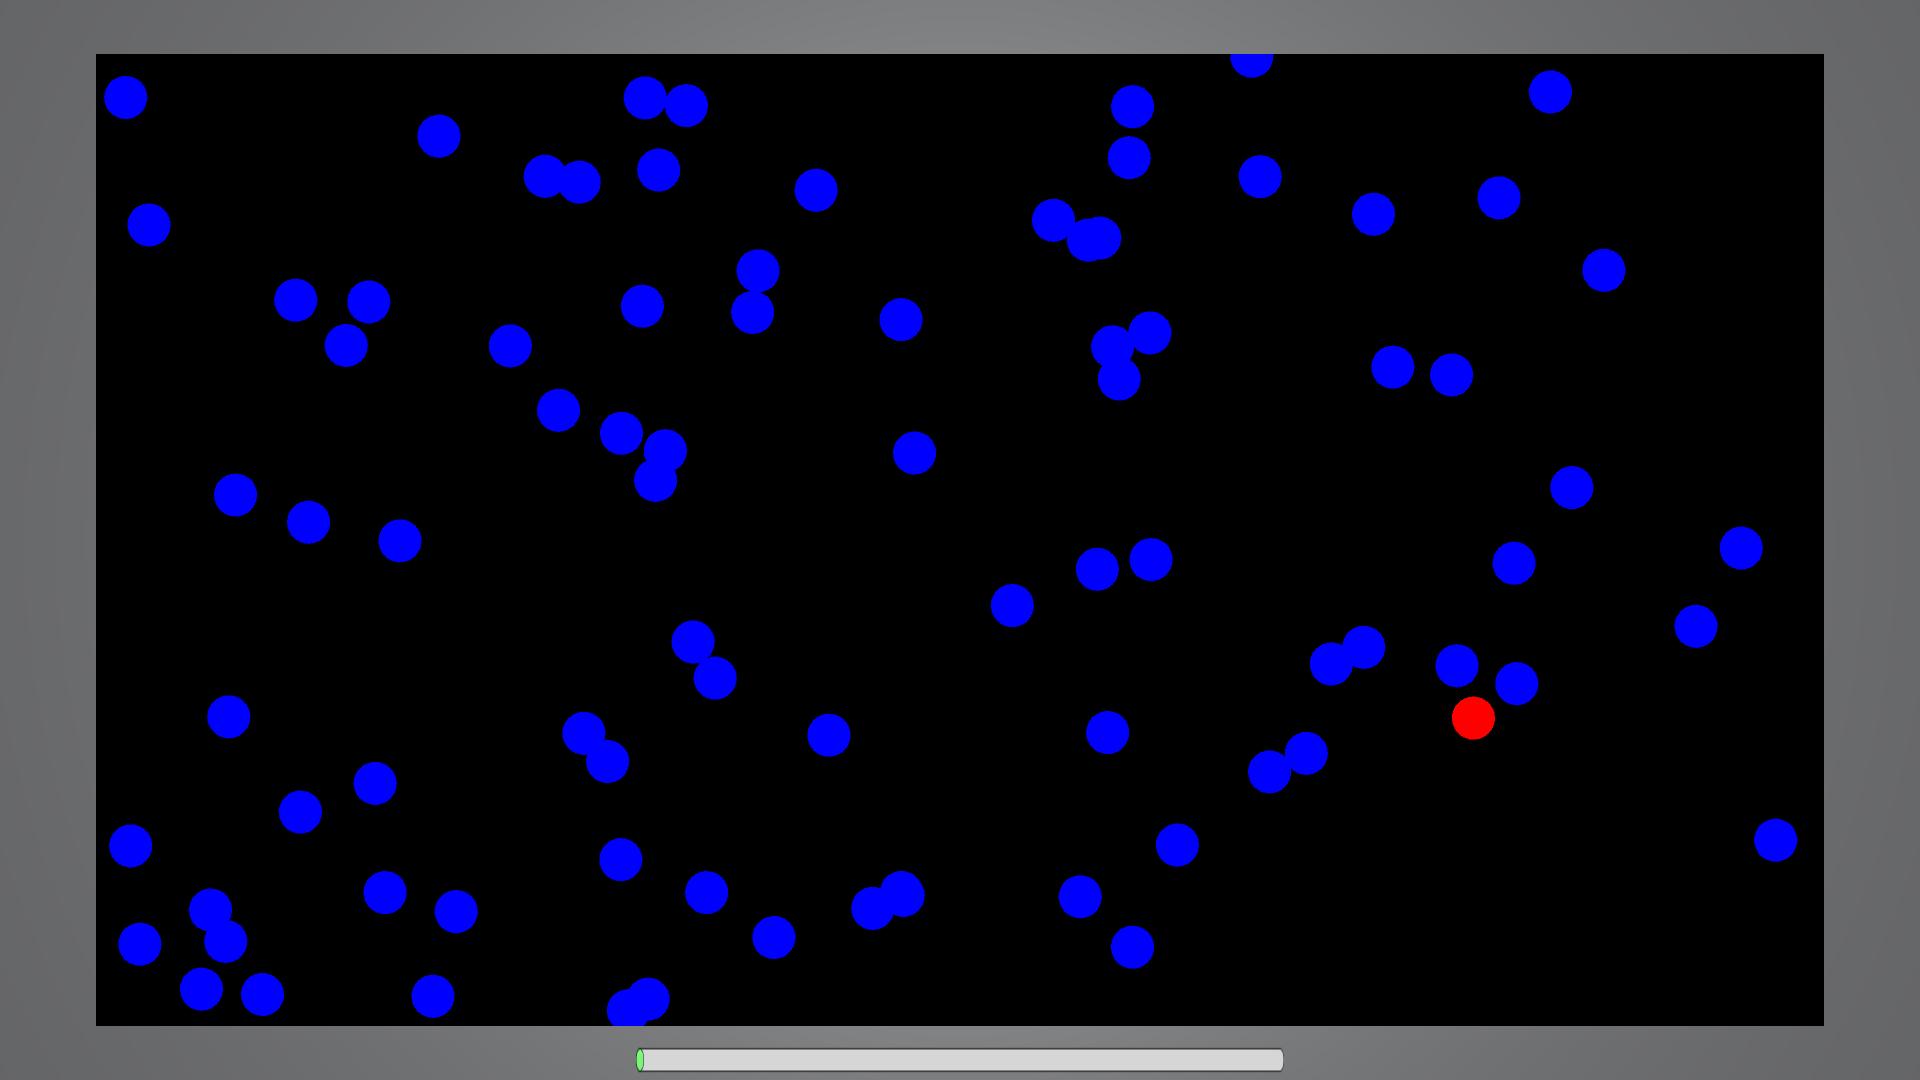
\includegraphics[width=0.7\textwidth]{figures/ch5/pseudohaptics}
		\caption[Évaluation de \emph{FastHook}]{\emph{FastHook} : les distracteurs sont très nombreux.}
		\label{fig:pseudohaptics}
	\end{figure}
	
	\subsubsection{Favoriser la précision}
	Surtout, pour évaluer l'intérêt de \emph{FastHook} dans les applications où la précision est critique, nous avons expressément demandé à nos sujets de favoriser très fortement la précision, c'est-à-dire de tâcher d'éviter les erreurs autant que possible. Nous supposons en effet que c'est dans de cas précis que \emph{FastHook} est susceptible de montrer son intérêt par rapport à la version standard de \emph{Hook}, car nous faisons l'hypothèse que la phase d'accrochage sera de faible durée par rapport à la phase de \emph{renforcement}, c'est-à-dire la phase pendant laquelle l'utilisateur continue de suivre la cible pour affermir son accrochage et éviter une erreur de sélection. Or, puisque nous supposons que \emph{FastHook} permettra spécifiquement de réduie cette phase de renforcement, nous pensons que c'est avec une stratégie fortement orientée vers la précision que cette technique peut se distinguer.

	
	\subsection{Résultats}
	Les résultats bruts et avec normalisation sont présentés sur la figure~\ref{fig:fastHookAllRes}. Examinons d'abord les résultast bruts. Premièrement, \emph{FastHook} n'a pas d'effet significatif sur les temps de sélection, à l'exception d'une augmentation de leur dispersion, qui se répercute logiquement sur $Perf$. Une très légère baisse des taux d'erreurs est observée.
	
	Sur les résultats normalisés, on constate toutefois une baisse significative des temps de sélection, qui suggère un bénéfice plus marqué chez les sujets relativement performants. La même baisse des taux d'erreurs est remarquée, quoique très légèrement plus marquée. De même, les $Perf$ moyennes baissent significativement.
	
	En réalité, l'examen global des résultats masque de très importantes différences entre les sujets, selon la mesure dans laquelle ils sont observé nos consignes concernant les taux d'erreurs. Nous avons donc choisi de réexaminer nos résultats en les séparant en deux groupes : ceux qui ont fait des erreurs d'une part, choisissant un compromis relativement orienté vers la vitesse, et ceux qui n'en ont fait aucune d'autre part, choisissant un compromis relativement orienté vers la précision. Il se trouve que chaque sous-groupe contient 4 sujets.
	
	
	\begin{figure}[!htb]
		\begin{subfigure}[t]{0.49\textwidth}
			\centering
			\includegraphics[width=\textwidth]{figures/ch5/phRawTimes}
			\caption{Temps de sélection bruts.}
			\label{fig:phRawTimes}
		\end{subfigure}
		~
		\begin{subfigure}[t]{0.49\textwidth}
			\centering
			\includegraphics[width=\textwidth]{figures/ch5/phRawErrors}
			\caption{Nombres moyens d'erreurs bruts.}
			\label{fig:phRawErrors}
		\end{subfigure}
		~
		\begin{subfigure}[t]{0.49\textwidth}
			\centering
			\includegraphics[width=\textwidth]{figures/ch5/phRawProducts}
			\caption{$\overline{Perf}$ brutes.}
			\label{fig:phRawProducts}
		\end{subfigure}
		~
		\begin{subfigure}[t]{0.49\textwidth}
			\centering
			\includegraphics[width=\textwidth]{figures/ch5/phNormTimes}
			\caption{MTSN.}
			\label{fig:phNormTimes}
		\end{subfigure}
				~
		\begin{subfigure}[t]{0.49\textwidth}
			\centering
			\includegraphics[width=\textwidth]{figures/ch5/phNormErrors}
			\caption{MTEN.}
			\label{fig:phNormErrors}
		\end{subfigure}
				~
		\begin{subfigure}[t]{0.49\textwidth}
			\centering
			\includegraphics[width=\textwidth]{figures/ch5/phNormProducts}
			\caption{$\overline{Perf}$ (avec normalisation).}
			\label{fig:phNormProducts}
		\end{subfigure}
		\caption[\emph{FastHook} -- résultats]{Performances de sélection de \emph{FastHook} -- résultats globaux, bruts et normalisés. Moyennes, intervalles de confiance à 95~\%{}.}
		\label{fig:fastHookAllRes}
	\end{figure}
	
	\subsubsection{Résultats du sous-groupe orienté vitesse}
	Les résultats du sous-groupe ayant relativement favorisé la vitesse sont présentés sur la figure~\ref{fig:fastHookSpRes}. Commençons à nouveau par les résultats bruts. Les temps de sélection augmentent de manière assez marquée, bien que les intervalles de confiance à 95~\%{} se chevauchent nettement. Les erreurs --- au demeurant rares, les sujets concernés ayant tout de même tenté de les minmiser un peu --- sont légèrement réduites, tandis que $Perf$ suit la tendance des temps de sélection.
	
	Les résultats normalisés présentent à peu près les mêmes tendances, mais la normalisation a pour effet de réduire les variations inter-sujets et, par conséquent, la dispersion des résultats. De fait, les intervalles de confiance sont plus étroits. Ici, \emph{FastHook} est clairement moins perfomant que la version standard de \emph{Hook}.

	\begin{figure}[!htb]
		\begin{subfigure}[t]{0.49\textwidth}
			\centering
			\includegraphics[width=\textwidth]{figures/ch5/phSpRawTimes}
			\caption{Temps de sélection bruts.}
			\label{fig:phSpRawTimes}
		\end{subfigure}
		~
		\begin{subfigure}[t]{0.49\textwidth}
			\centering
			\includegraphics[width=\textwidth]{figures/ch5/phSpRawErrors}
			\caption{Nombres moyens d'erreurs bruts.}
			\label{fig:phSpRawErrors}
		\end{subfigure}
		~
		\begin{subfigure}[t]{0.49\textwidth}
			\centering
			\includegraphics[width=\textwidth]{figures/ch5/phSpRawProducts}
			\caption{$\overline{Perf}$ brutes.}
			\label{fig:phSpRawProducts}
		\end{subfigure}
		~
		\begin{subfigure}[t]{0.49\textwidth}
			\centering
			\includegraphics[width=\textwidth]{figures/ch5/phSpNormTimes}
			\caption{MTSN.}
			\label{fig:phSpNormTimes}
		\end{subfigure}
				~
		\begin{subfigure}[t]{0.49\textwidth}
			\centering
			\includegraphics[width=\textwidth]{figures/ch5/phSpNormErrors}
			\caption{MTEN.}
			\label{fig:phSpNormErrors}
		\end{subfigure}
				~
		\begin{subfigure}[t]{0.49\textwidth}
			\centering
			\includegraphics[width=\textwidth]{figures/ch5/phSpNormProducts}
			\caption{$\overline{Perf}$ (avec normalisation).}
			\label{fig:phSpNormProducts}
		\end{subfigure}
		\caption[\emph{FastHook} -- résultats II]{Performances de sélection de \emph{FastHook} -- résultats du groupe orienté vitesse, bruts et normalisés. Moyennes, intervalles de confiance à 95~\%{}, et 99~\%{} (moustaches).}
		\label{fig:fastHookSpRes}
	\end{figure}
	
	\subsubsection{Résultats du sous-groupe orienté précision}
	Les résultats du sous-groupe ayant relativement favorisé la vitesse sont présentés sur la figure~\ref{fig:fastHookPrRes}. Nous nous contentons ici de rapporter les temps de sélection, car ces sujets n'ont commis aucune erreur, ce qui implique des valeurs de $Perf$ identiques aux temps de sélection. Les résultats bruts et normalisés sont à peu près identiques, et montre un avantage très net pour \emph{FastHook}, qui permet de réduire les temps de sélection d'environ 26 à 27~\%{}.
	
	\begin{figure}[!htb]
		\begin{subfigure}[t]{0.49\textwidth}
			\centering
			\includegraphics[width=\textwidth]{figures/ch5/phPrRawTimes}
			\caption{Temps de sélection bruts.}
			\label{fig:phPrRawTimes}
		\end{subfigure}
		~
		\begin{subfigure}[t]{0.49\textwidth}
			\centering
			\includegraphics[width=\textwidth]{figures/ch5/phPrNormTimes}
			\caption{MTSN.}
			\label{fig:phPrNormTimes}
		\end{subfigure}
		\caption[\emph{FastHook} -- résultats III]{Performances de sélection de \emph{FastHook} -- résultats du groupe orienté précision, bruts et normalisés. Moyennes, intervalles de confiance à 95~\%{} (boîtes), et 99~\%{} (moustaches).}
		\label{fig:fastHookPrRes}
	\end{figure}
	

	\subsubsection{Corrélations}
	Le tableau~\ref{tab:fastHookCorr} rapporte quelques-unes des corrélations observées au cours de notre étude portant sur \emph{FastHook}. D'une part, la normalisation des résultats tend à renforcer les corrélations, nous l'avons déjà vu et expliqué. D'autre part, il est intéressant de constater que notre estimation de la difficulté prédit mieux les performances de sélection du sous-groupe orienté précision que de celui orienté vitesse. Nous n'avons pas à ce jour d'explication satisfaisante à ce phénomène, qui devra faire l'objet d'études plus approfondies. En tout état de cause, cette corrélation est très forte pour le sous-groupe orienté précision.
	
	Nous ne les détaillons pas sur ce tableau, mais d'intéressantes anti-corrélations existent entre l'amplitude des angles de rotation et les temps de sélection. Notamment, dans le sous-groupe orienté précision, elle atteint -38,09~\%{}, avec une \emph{p-value} de 6,5$.10^{-25}$. Nous supposons qu'elle est liée au fait que les cibles dont le paramètre A est élevé tendent à avoir un mouvement brownien, surtout si F est également élevé (une anti-corrélation similaire est observée avec F, mais elle est moins marquée). Dans ce cas, la vitesse extrême des cibles est moins gênante, car leur déplacement total sur une fenêtre temporelle d'une seconde (par exemple) est faible. De fait, les \og suivre \fg{} avec \emph{Hook} est assez facile.
	
	Dans toutes les conditions et tous les sous-groupes, avec ou sans normalisation, les valeurs absolues des corrélations entre A ou F d'une part, et les performances de sélection d'autre part, sont nettement inférieures à celles entre notre estimation de la difficulté d'une part, et les performances de sélection d'autre part. La vitesse étant constante dans cette étude, il est impossible de mesurer une corrélation entre V et les performances de sélection. Avec cette réserve, nous pouvons retenir notre hypothèse \textbf{H5}.
	
	
\begin{table}
	\centering
	\begin{tabular}{l | c c c c}
		Condition				& C($d$, $T$)			& C($d$, $E$)			& C($d$, $Perf$)		\bigstrut[b] \\ \hline
		\emph{Hook} (G)			& 29,75 ; 7$.10^{-29}$	& 10,61 ; 9$.10^{-5}$	& 21,05 ; 4$.10^{-15}$	\bigstrut[t] \\
		\emph{FastHook} (G)		& 11,86 ; $10^{-5}$		& 13,74 ; 4$.10^{-7}$	& 8,43 ; 0,002			\\
		\emph{Hook} (Gn)		& 38,83 ; 4$.10^{-50}$	& 10,99 ; 5$.10^{-5}$	& 39,31 ; 4$.10^{-51}$	\\
		\emph{FastHook} (Gn)	& 37,22 ; 6$.10^{-46}$	& 14,13 ; 2$.10^{-7}$	& 36,81 ; 7$.10^{-45}$	\\
		\emph{Hook} (V)			& 22,64 ; 2$.10^{-9}$	& 15,56 ; 5$.10^{-5}$	& 18,73 ; 9$.10^{-7}$	\\
		\emph{FastHook} (V)		& 11,29 ; 0,003			& 19,92 ; 2$.10^{-7}$	& 9,21 ; 0,016			\\
		\emph{Hook} (Vn)		& 34,11 ; 5$.10^{-20}$	& 16,09 ; 2$.10^{-5}$	& 31,42 ; 5$.10^{-17}$	\\
		\emph{FastHook} (Vn)	& 32,34 ; 5$.10^{-18}$	& 20,50 ; 7$.10^{-8}$	& 31,73 ; 2$.10^{-17}$	\\
		\emph{Hook} (Pr)		& 61,72 ; $10^{-72}$	& --					& 61,72 ; $10^{-72}$	\\
		\emph{FastHook} (Pr)	& 50,38 ; 5$.10^{-45}$	& --					& 50,38 ; 5$.10^{-45}$	\\
		\emph{Hook} (Prn)		& 60,07 ; 6$.10^{-68}$	& --					& 60,07 ; 6$.10^{-68}$	\\
		\emph{FastHook} (Prn)	& 46,76 ; 3$.10^{-38}$	& --					& 46,76 ; 3$.10^{-38}$	\\
	\end{tabular}
	\caption[\emph{Hook} et \emph{FastHook} -- corrélations]{Corrélations (exprimées en pourcentages) entre l'estimation de la difficulté $d$ d'une part, les temps de sélection $T$, les taux d'erreurs $E$, et les $Perf$ d'autre part. G = résultats globaux, V = résultats du sous-groupe orienté vitesse, Pr = résultats du sous-groupe orienté précision. L'ajout d'un \emph{n} indique des résultats normalisés.}
	\label{tab:fastHookCorr}
\end{table}
	
	
	\subsection{Interprétation}
	La nature hétérogène de nos résultats impose une interprétation minutieuse et prudente. Comme nous l'avons vu, la stratégie choisie par les sujets interagit de manière significative avec l'influence de \emph{FastHook} sur les performances de sélection. Lorsque l'accent mis sur la précision n'est pas très fort, \emph{FastHook} augmente les temps de sélection, sans effet significatif sur les taux d'erreurs. Lorsque les sujets privilégient fortement la précision, en tâchant d'éviter toute erreur, alors les temps de sélection sont fortement diminués avec \emph{FastHook}.
	
	Or, avec une technique de type \emph{Hook}, mettre l'accent sur la précision consiste essentiellement à suivre une cible pendant un moment une fois qu'elle est accrochée, jusqu'à s'être assuré qu'elle l'est \og fermement \fg{}. C'est précisément cette phase que l'assistance pseudo-haptique facilite, en rapprochant le curseur de la cible, parfois au point de l'y \og coller \fg{}  définitivement. Lorsque cela se produit, l'utilisateur peut cliquer en toute confiance, sans avoir besoin de poursuivre la cible pendant longtemps. C'est le mécanisme principal par lequel \emph{FastHook} peut réduire les temps de sélection. Ajoutons cependant que, parfois, l'assistance pseudo-haptique ne permet pas de coller le curseur à la cible, mais l'en rapproche significativement, ce qui permet un accrochage plus ferme dans un laps de temps donné. Attenu que nous avons expliqué le fonctionnement de \emph{Hook} à nos sujets, ils ont également pu exploiter cet effet.
	
	Les sujets n'ayant pas trop cherché à favoriser la précision, en revanche, n'ont pas passé beaucoup de temps à poursuivre la cible \emph{après} l'avoir accrochée, et c'est ce qui explique leurs erreurs (toutefois rares) : la cible pouvait se décrocher entre la décision de cliquer et le clic effectif. De fait, le temps d'accrochage était, pour ces sujets, bien plus long que le temps de renforcement de l'accrochage. Or, au cours de ce premier, l'assistance pseudo-haptique n'est d'aucune aide, puisqu'elle attire le curseur vers un distracteur : elle constitue même une gêne. De fait, le temps d'accrochage est accru, et les performances globales chutent.
	
	En somme, \emph{FastHook} est à privilégier lorsqu'il est impératif de minimiser les taux d'erreurs, voire de les annuler. Dans le cas contraire, il est plutôt délétère. Notons toutefois que l'assistance pseudo-haptique utilisée ici était forte, suffisamment pour suivre une cible extrêmement rapide sans intervention aucune de l'utilisateur (pour une valeur de $f_{accrochage}$ suffisamment élevée --- voir l'équation~\ref{eq:phDisplacement2}). Une assitance plus faible pourrait avoir des effets différents sur les performances de sélection. Nous pouvons donc retenir notre hypothèse \textbf{H6} (via sa composante \textbf{H6a}) lorsque la stratégie est très orientée vers la précision, et la rejeter dans le cas contraire. Dans tous les cas, la composante \textbf{H6b} doit être rejetée, puisque les taux d'erreurs ne baissent pas significativement avec une stratégie orientée vitesse, et sont toujours nuls avec une stratégie orientée précision.
	
	\section{Cascade et prédiction intentionnelle -- \emph{BaggingHook}}
	Les performances de \emph{Hook} dans sa version de base sont très bonnes. Certes, les temps de sélection rapportés sur la figure~\ref{fig:phRawTimes} sont élevés, mais c'est à mettre en rapport avec l'extrême difficulté de la tâche d'une part, et avec le fait que \emph{Hook}, contrairement à de nombreuses techniques de sélection, n'augmente que peu l'encombrement visuel (et même pas du tout dans la version que nous évaluons ici), n'interromp pas le temps, ni même ne le ralentit, et n'altère pas les mouvements des cibles. Il ne cause pas non plus la moindre perte de contexte spatial ou dynamique. En somme, il a un impact quasi nul sur le contexte applicatif, visuellement, spatialement ou temporellement.
	
	La difficulté de la tâche tient essentiellement à deux facteurs : les mouvements des cibles d'une part, et leur forte densité d'autre part. En effet, la technique \emph{Hook} cherche à déterminer quel objet l'utilisateur est en train d'essayer d'attraper en analysant ses mouvements et en les comparant à ceux des cibles potentielles. Or, quand la densité est élevée, il devient probable qu'un distracteur aient des positions plus fortement corrélées à celle du curseur que celles de la cible visée. Dans ce cas, l'heuristique peine à \og accrocher \fg{} la bonne cible. Ce problème ne se pose de manière sérieuse que lorsque la forte densité est conjugée à des mouvements difficiles (rapides et imprévisibles), car lorsque la densité est très élevée mais les mouvements sont lents ou prévisibles, il devient relativement aisé de suivre la cible de près, ce qui permet à l'heuristique de l'identifier correctement.
	
	Par conséquent, une piste possible pour faciliter la sélection lorsque les mouvements sont difficiles et la densité est forte est de simplifier la nature des mouvements, par exemple en s'appuyant sur une des méthodes proposées dans la section~\ref{sub:vfaGuide}. Mais il est également possible de réduire la densité (effective). Nous avons vu dans la section~\ref{sub:cascade} que la sélection en cascade vise généralement à découper la tâche de sélection en sous-tâches, permettant de réduire le nombre d'objets (ou de paquets d'objets) à sélectionner au cours de chaque sous-tâche. Toutefois, la plupart des techniques passées en revue dans cette section ont des inconvénients incompatibles avec les objectifs que nous nous sommes fixées, compte tenu des contraintes applicatives identifiées dans le chapitre~\ref{chap1}. Elles entraînent généralement une perte de contexte spatial ou dynamique, et peuvent même être fondamentalement incompatible avec des cibles mobiles. De plus, elles impliquent le plus souvent l'obligation de diviser la tâche en plusieurs parties, ce qui a nécessairement un coût cognitif et temporel. Celui-ci est généralement rentabilisé, mais pas toujours.
	
	\subsection{\emph{BaggingHook}, ou l'élagage optionnel et à volonté}
	L'amélioration des performances d'une technique fondée sur \emph{Hook} reposerait donc idéalement sur une méthode permettant de réduire le nombre de cibles potentielles pour faciliter la convergence de l'heuristique de prédiction vers la bonne cible, mais sans occasionner de perte du contexte, et sans imposer d'étape préalable à la sélection. Nous proposons donc \emph{BaggingHook}, qui ajoute au curseur ponctuel de \emph{Hook} un curseur zonal circulaire, permettant, via le bouton secondaire de la souris\footnote{De fait inutilisable pour réinitialiser les scores.}, de retirer tous les objets non inclus dans son rayon de la liste des cibles potentielles considérées par l'heuristique de prédiction. Cette opération peut être répétée à l'envi, afin d'exclure autant de cibles que possible\ldots{} ou ne pas être utilisée du tout, afin de ne pas imposer d'étape supplémentaire dans la sélection. Ce dernier point est particulièrement intéressant pour les cibles faciles ne nécessitant pas cet élagage, car le coût cognitif et temporel qui lui est associé pourrait s'avérer globalement délétère. D'un certain point de vue, \emph{BaggingHook} s'apparente au \emph{Rake cursor}~\cite{blanch2009rake}, puisque les deux phases de la sélection sont menées simultanément, l'heuristique de prédiction continuant à fonctionner pendant les éventuels élagages.
	
	Ce procédé a néanmoins un inconvénient, puisqu'il est possible de \og rater \fg{} son élagage, c'est-à-dire de retirer la bonne cible de la liste des objets potentiels. Nous aurions pu considérer un tel événement comme une erreur et, par exemple, réintégrer tous les objets dans la liste des cibles potentielles automatiquement dans ce cas. Nous estimons cependant que, dans bien des applications, une sélection erronée peut avoir des effets indésirables (effets graphiques perturbants, action subséquente automatique\ldots{}), tandis qu'un élagage erroné, s'il est réversible, n'a pour inconvénient que de prendre du temps. Nous avons donc décider de fournir à nos utilisteurs la possibilité de réintégrer tous les objets à la liste des cibles potentielles par la pression de la touche R du clavier (pour \emph{Reset}), et de ne pas considérer cela comme une erreur.
	
	Il pourrait être préférable de plutôt associer cette touche à une fonction d'annulation du dernier élagage opéré, permettant de revenir à l'état antérieur de la liste des cibles potentielles. Pour simplifier cette première évaluation du potentiel de \emph{BaggingHook}, nous avons préféré la solution de réinitialisation, ayant le mérite d'une part d'être plus simple, et d'autre part de ne nécessiter qu'une seule action, tandis que plusieurs retours successifs aux états antérieurs pourraient être nécessaire, en cas de multiples élagages erronés, parfaitement possible avec un utilisateur faisant un usage intensif de cette fonction.
	
	
	\subsection{Retour graphique associé à l'élagage}
	Lorsque l'utilisateur déclenche un élagage, il importe de lui fournir un retour lui permettant de mesurer l'effet de l'opération. Il est possible, par exemple, de rendre toutes les cibles élagées semi-transparentes, ou de les assombrir, ce qui pose la question du niveau d'opacité dans le premier cas, ou de la mesure de l'assombrissement dans le second. Dans un souci de simplicité, nous avons simplement rendu les cibles élagées invisibles. Gardons simplement à l'esprit que, selon le contexte, il peut être nécessaire de les maintenir à l'écran, qu'elles soient transparentes, sombres, ou altérées d'une autre manière.
	
	\subsection{Résultats}
	
	\subsection{Biais et zone d'élagage ajustable}
	Pertinence du biais ? Peu de corrélation diff-temps
	
	Mais forte anticorrélation area-culls
		Donc zone d'élagage petite avec petites aires ?
		Et périmètres ?
		Non aires.
	
	\subsection{Inconvénients}
	Charge cognitive, doute stratégique.
	
	Perspective : biais brownien ?
	
	\section{Limites de \emph{Hook} et de ses dérivés}
	Certes, la technique \emph{Hook} fournit d'excellentes performances, et nos dérivés peuvent les améliorer encore. Certes, les principes sur lesquels \emph{SharpHook} et \emph{FastHook} reposent peuvent être combinés, et leur mise en œuvre peut être améliorée et calibrée avec plus grand soin. Certes, d'autres techniques, telles que celles évoquées dans la section~\ref{sub:vfaGuide} peuvent encore s'y ajouter. Néanmoins, dans le cadre de l'utilisation d'un dispositif de type CAVE avec un dispositif d'interaction à l'échelle 1, l'utilisation d'une technique de ce type impose à l'utilisateur de suivre la cible en bougeant son bras à une vitesse approximativement comparable. Si la cible se déplace sur plus de quelques dizaines de centimètres, il devient alors nécessaire de déplacer tout son corps à cette vitesse.
	
	Or, nous avons évalué \emph{FastHook} dans un contexte où des cibles d'environ 1~cm de diamètre se meuvent à environ 40~cm/s. Une simple règle de trois fournit un équivalent possible dans un grand environnement immersif : des cibles de 10~cm de diamètre se déplaçant à 4~m/s, soit près de 15~km/h. Il s'agit là d'un rythme de course à pied relativement soutenu, et il nous apparaît clair que se déplacer de manière continue à cette vitesse pour interagir avec des cibles, et en changeant constamment de direction de surcroît, serait extrêmement fatigant, et intolérable sur plus de quelques secondes. Aussi devons-nous rejeter \emph{Hook} et ses dérivés pour des applications aussi extrêmes.
	
	En revanche, l'ensemble des idées évoquées et éventuellement évaluées dans ce chapitre sont compatibles avec une technique de type \emph{IntenSelect}~\cite{de2005intenselect} (décrite dans la section~\ref{sub:intenSelect}). Or, celle-ci ne nécessite pas de déplacer le dispositif d'interaction, mais simplement d'y appliquer des rotations. Sans doute des limites physiques existent-elles aussi pour les mouvements de ce type, mais nous supposons qu'elles sont moins rapidement atteintes, puisque la masse corporelle déplacée est bien plus faible, de même que la force exercée. Nous préconisons donc d'utiliser les variantes de \emph{Hook} que nous proposons lorsque c'est possible, mais d'opter pour des variantes correspondantes fondées sur \emph{IntenSelect} dans les autres cas.
	
	\section{Métrique synthétique paramétrable}
	Dans la section~\ref{sub:product}, nous avons introduit une métrique synthétique permettant d'évaluer les performances de sélection d'un sujet ou d'une technique en la réduisant à un seul nombre, appelé $Perf$, avec $Perf = T(E+1)$ où $T$ est le temps de sélection et $E$ le nombre d'erreurs. En réalité, cette formule assez simple cache un parti pris assez fort : celui d'accorder un poids égal au temps de sélection et aux erreurs. En effet, on peut voir cette formule comme un cas particulier d'une forme plus générale : $Perf(m,n) = T^{m}(E+1)^{n}$ avec $m, n \in \mathbb{R}^{+}$.
	
	En pratique, sans doute n'est-il pas nécessaire de chercher à ajuster les deux exposants, car il suffit d'en modifier un pour altérer le poids relatif du facteur auquel il s'applique. On peut donc réduire cette formule à $Perf(m,n) = T(E+1)^{n}$. On pourra ainsi diminuer l'influence du taux d'erreurs sur les performances en diminuant $n$, et vice-versa. Dans un souci de praticité, nous proposons de se référer à un paramètre $p$, pour \emph{précision}, défini par $p = \log_2\left(n\right)$. Cela permet d'avoir un paramètre d'effet symétrique, et centré sur 0. Par exemple, nous avons les couples $(p,n)$ suivants : $\left(0,1\right), \left(1,2\right), \left(-1,\frac{1}{2}\right), \left(2,4\right), \left(-2,\frac{1}{4}\right)$\ldots{} Plus généralement, le facteur $E+1$ sera élevé à la puissance $2^{p}$ si $p$ est positif, ou remplacé par sa racine $2^{\abs*{p}}$-ième si $p$ est négatif.
	
	\section{Améliorer l'estimation de la difficulté de sélection}
	Notre modèle d'estimation de la difficulté de sélection fournit des résultats cohérents et fiables, nous l'avons vu. Cependant, il n'est pas sans faiblesses, comme l'illustre par exemple la différence entre les figures~\ref{fig:perf_V_RealArea_lousy_fit} et~\ref{fig:perf_V_RealArea_better_fit}, qui met en lumière le manque de précision de notre modèle lorsque la valeur de F est particulièrement basse.
	
	Sans doute serait-il possible d'améliorer l'estimation de la difficulté de sélection d'une cible ; c'est du moins ce que suggèrent les valeurs de nos corrélations résumées par le tableau~\ref{tab:synthRes}, qui montrent une certaine marge de progression. Une modélisation mathématique plus astucieuse serait probablement utile, de même que des données plus variées et plus nombreuses afin de l'étalonner. En particulier, il pourrait être opportun de créer des modèles spécifiques à chaque paradigme de sélection (prédiction intentionnelle, augmentation des cibles, assistance haptique ou pseudo-haptique, etc.) afin d'en améliorer la précision et l'utilité (voir les tableaux~\ref{tab:hookCorr} et~\ref{tab:fastHookCorr}).
	
	\subsection{Réseaux de neurones}
	Une méthode radicalement différente consisterait à employer un procédé d'apprentissage machine, tel qu'un réseau de neurones. Les entrées du réseau devraient inclure V, F, et A, voire également la largeur W et la distance D du modèle classique de Fitts, que nous avons souvent omis dans ces travaux, en les fixant, pour limiter le focus --- déjà très large --- des études menées. Nous pourrions également y ajouter le coefficient d'autocorrélation, décrit dans la section~\ref{sub:vfaMem}. La sortie du réseau serait tout simplement une estimation de la difficulté de sélection de la cible concernée. Il est probable qu'un tel réseau, nourri de suffisamment de données d'apprentissage, fournirait une estimation nettement plus fiable, et donc potentiellement plus utile, de la difficulté inhérente à la sélection d'une cible mobile.
	
	Certes, les réseaux de neurones ont parfois l'inconvénient d'être comparables à des \og boîtes noires \fg{}, permettant difficilement de comprendre pourquoi et comment ils aboutissent à un résultat donné. En ce sens, ils pourraient être plus difficiles à appréhender pour la conception de paradigmes de sélection. Néanmoins, nous demeurons convaincus de l'intérêt de poursuivre cette piste dans de futurs travaux.
	
	\section{Conclusion}
	Dans la première partie de ce chapitre, nous avons exposé plusieurs méthodes permettant de faciliter la sélection de cibles mobiles en jouant sur leurs paramètres VFA, soit directement, soit à l'aide de \emph{proxies}, ou en lissant simplement les trajectories. Nous avons estimé quantitativement les effets de ces méthodes sur la nature des mouvements des objets concernés, et avons examiné les mérites respectifs de ces différents procédés.
	
	Nous avons proposé de mêler la prédiction intentionnelle à l'utilisation sporadique de \emph{proxies} afin de limiter l'encombrement visuel généré, et nous avons souligné l'intérêt de mêler tous ces procédés à des techniques de sélection existantes et éprouvées, éventuellement améliorées.
	
	Puis, dans la deuxième partie du chapitre, nous avons étudié la relation entre la distance de Fitts et les performances de sélection de cibles mobiles, montrant que l'influence de la première sur les secondes était très faible, tout au plus. Puis, nous avons évalué la possibilité d'utiliser l'estimation de la difficulté de sélection d'une cible pour en ajuster la taille afin d'améliorer les performances de sélection globale. Pour ce faire, nous avons mené une étude empirique avec 16 participants. Celle-ci a permis de valider l'efficacité de notre prédiction de la difficulté de sélection, et de montrer que les performances pouvaient être améliorées en ajustant les tailles des cibles, de même que l'homogénéité des performances en question. Surtout, nos résultats ouvrent de nombreuses perspectives pour le développement de paradigmes de sélection, puisqu'ils mettent en lumière la possibilité d'utiliser la difficulté de sélection d'une cible soit pour en ajuster la taille en combinaison avec une technique d'aide à la sélection efficace, soit pour biaiser une heuristique de prédiction intentionnelle.
	
	C'est justement ce que nous avons évalué dans la troisième partie de ce chapitre, avec 8 participants. Nous avons montré que ce biais permet d'améliorer légèrement --- mais significativement --- les temps de sélection et les taux d'erreurs, en comparant notre technique biaisée, que nous appelons \emph{SharpHook}, à la technique \emph{Hook}~\cite{ortega2013hook}.
	
	Dans la quatrième partie, nous avons évalué l'intérêt d'une assistance pseudo-haptique utilisée en conjonction avec \emph{Hook} dans sa version non biaisée. Nous avons observé que, selon la stratégie des utilisateurs, cette assistance peut avoir un effet bénéfique ou délétère. Nous appelons cette nouvelle technique \emph{FastHook}.
	
	Nous signalons par ailleurs que l'usage de tels procédés est compatible avec les lissages et filtrages décrits dans la première partie. Nous proposons également une métrie paramétrable pour quantifier les performances de sélection en ajustant la pondération des temps de sélection et des erreurs.
	
	Enfin, nous avons critiqué notre modèle de prédiction de la difficulté de sélection, et proposé une piste pour obtenir des résultats plus précis et plus fiables, afin de mieux contribuer aux performances de sélection, dans le cadre d'un paradigme combinant plusieurs procédés.